\documentclass[twoside]{book}

% Packages required by doxygen
\usepackage{calc}
\usepackage{doxygen}
\usepackage{graphicx}
\usepackage[utf8]{inputenc}
\usepackage{makeidx}
\usepackage{multicol}
\usepackage{multirow}
\usepackage{textcomp}
\usepackage[table]{xcolor}

% Font selection
\usepackage[T1]{fontenc}
\usepackage{mathptmx}
\usepackage[scaled=.90]{helvet}
\usepackage{courier}
\usepackage{amssymb}
\usepackage{sectsty}
\renewcommand{\familydefault}{\sfdefault}
\allsectionsfont{%
  \fontseries{bc}\selectfont%
  \color{darkgray}%
}
\renewcommand{\DoxyLabelFont}{%
  \fontseries{bc}\selectfont%
  \color{darkgray}%
}

% Page & text layout
\usepackage{geometry}
\geometry{%
  a4paper,%
  top=2.5cm,%
  bottom=2.5cm,%
  left=2.5cm,%
  right=2.5cm%
}
\tolerance=750
\hfuzz=15pt
\hbadness=750
\setlength{\emergencystretch}{15pt}
\setlength{\parindent}{0cm}
\setlength{\parskip}{0.2cm}
\makeatletter
\renewcommand{\paragraph}{%
  \@startsection{paragraph}{4}{0ex}{-1.0ex}{1.0ex}{%
    \normalfont\normalsize\bfseries\SS@parafont%
  }%
}
\renewcommand{\subparagraph}{%
  \@startsection{subparagraph}{5}{0ex}{-1.0ex}{1.0ex}{%
    \normalfont\normalsize\bfseries\SS@subparafont%
  }%
}
\makeatother

% Headers & footers
\usepackage{fancyhdr}
\pagestyle{fancyplain}
\fancyhead[LE]{\fancyplain{}{\bfseries\thepage}}
\fancyhead[CE]{\fancyplain{}{}}
\fancyhead[RE]{\fancyplain{}{\bfseries\leftmark}}
\fancyhead[LO]{\fancyplain{}{\bfseries\rightmark}}
\fancyhead[CO]{\fancyplain{}{}}
\fancyhead[RO]{\fancyplain{}{\bfseries\thepage}}
\fancyfoot[LE]{\fancyplain{}{}}
\fancyfoot[CE]{\fancyplain{}{}}
\fancyfoot[RE]{\fancyplain{}{\bfseries\scriptsize Generated on Mon Dec 1 2014 23\-:33\-:04 for Munchkin by Doxygen }}
\fancyfoot[LO]{\fancyplain{}{\bfseries\scriptsize Generated on Mon Dec 1 2014 23\-:33\-:04 for Munchkin by Doxygen }}
\fancyfoot[CO]{\fancyplain{}{}}
\fancyfoot[RO]{\fancyplain{}{}}
\renewcommand{\footrulewidth}{0.4pt}
\renewcommand{\chaptermark}[1]{%
  \markboth{#1}{}%
}
\renewcommand{\sectionmark}[1]{%
  \markright{\thesection\ #1}%
}

% Indices & bibliography
\usepackage{natbib}
\usepackage[titles]{tocloft}
\setcounter{tocdepth}{3}
\setcounter{secnumdepth}{5}
\makeindex

% Hyperlinks (required, but should be loaded last)
\usepackage{ifpdf}
\ifpdf
  \usepackage[pdftex,pagebackref=true]{hyperref}
\else
  \usepackage[ps2pdf,pagebackref=true]{hyperref}
\fi
\hypersetup{%
  colorlinks=true,%
  linkcolor=blue,%
  citecolor=blue,%
  unicode%
}

% Custom commands
\newcommand{\clearemptydoublepage}{%
  \newpage{\pagestyle{empty}\cleardoublepage}%
}


%===== C O N T E N T S =====

\begin{document}

% Titlepage & ToC
\hypersetup{pageanchor=false}
\pagenumbering{roman}
\begin{titlepage}
\vspace*{7cm}
\begin{center}%
{\Large Munchkin }\\
\vspace*{1cm}
{\large Generated by Doxygen 1.8.6}\\
\vspace*{0.5cm}
{\small Mon Dec 1 2014 23:33:04}\\
\end{center}
\end{titlepage}
\clearemptydoublepage
\tableofcontents
\clearemptydoublepage
\pagenumbering{arabic}
\hypersetup{pageanchor=true}

%--- Begin generated contents ---
\chapter{Hierarchical Index}
\section{Class Hierarchy}
This inheritance list is sorted roughly, but not completely, alphabetically\-:\begin{DoxyCompactList}
\item \contentsline{section}{Carte}{\pageref{class_carte}}{}
\begin{DoxyCompactList}
\item \contentsline{section}{Comportement}{\pageref{class_comportement}}{}
\begin{DoxyCompactList}
\item \contentsline{section}{Carte\-Sup\-Main}{\pageref{class_carte_sup_main}}{}
\item \contentsline{section}{Malus\-Bonus}{\pageref{class_malus_bonus}}{}
\item \contentsline{section}{Malus\-Bonus\-Deguerpir}{\pageref{class_malus_bonus_deguerpir}}{}
\item \contentsline{section}{Perte\-Gain\-Niv}{\pageref{class_perte_gain_niv}}{}
\item \contentsline{section}{Perte\-Obj\-Max}{\pageref{class_perte_obj_max}}{}
\end{DoxyCompactList}
\item \contentsline{section}{Porte}{\pageref{class_porte}}{}
\begin{DoxyCompactList}
\item \contentsline{section}{Malediction}{\pageref{class_malediction}}{}
\item \contentsline{section}{Monstre}{\pageref{class_monstre}}{}
\item \contentsline{section}{Race}{\pageref{class_race}}{}
\end{DoxyCompactList}
\item \contentsline{section}{Tresor}{\pageref{class_tresor}}{}
\begin{DoxyCompactList}
\item \contentsline{section}{Equipement}{\pageref{class_equipement}}{}
\begin{DoxyCompactList}
\item \contentsline{section}{Armure}{\pageref{class_armure}}{}
\item \contentsline{section}{Chaussure}{\pageref{class_chaussure}}{}
\item \contentsline{section}{Couvre\-Chef}{\pageref{class_couvre_chef}}{}
\item \contentsline{section}{Main}{\pageref{class_main}}{}
\end{DoxyCompactList}
\item \contentsline{section}{Potion}{\pageref{class_potion}}{}
\end{DoxyCompactList}
\end{DoxyCompactList}
\item \contentsline{section}{Etat\-Joueur}{\pageref{class_etat_joueur}}{}
\begin{DoxyCompactList}
\item \contentsline{section}{Attente}{\pageref{class_attente}}{}
\item \contentsline{section}{Bagarre}{\pageref{class_bagarre}}{}
\item \contentsline{section}{Debut\-Tour}{\pageref{class_debut_tour}}{}
\item \contentsline{section}{Fin\-Tour}{\pageref{class_fin_tour}}{}
\item \contentsline{section}{Ouvrir\-Porte}{\pageref{class_ouvrir_porte}}{}
\end{DoxyCompactList}
\item \contentsline{section}{Fabrique}{\pageref{class_fabrique}}{}
\begin{DoxyCompactList}
\item \contentsline{section}{Fabrique\-Carte}{\pageref{class_fabrique_carte}}{}
\begin{DoxyCompactList}
\item \contentsline{section}{Fabrique\-Porte}{\pageref{class_fabrique_porte}}{}
\item \contentsline{section}{Fabrique\-Tresor}{\pageref{class_fabrique_tresor}}{}
\end{DoxyCompactList}
\item \contentsline{section}{Fabrique\-Comportement}{\pageref{class_fabrique_comportement}}{}
\end{DoxyCompactList}
\item \contentsline{section}{Munchkin}{\pageref{class_munchkin}}{}
\item \contentsline{section}{Personnage}{\pageref{class_personnage}}{}
\begin{DoxyCompactList}
\item \contentsline{section}{Joueur}{\pageref{class_joueur}}{}
\item \contentsline{section}{Monstre}{\pageref{class_monstre}}{}
\end{DoxyCompactList}
\end{DoxyCompactList}

\chapter{Class Index}
\section{Class List}
Here are the classes, structs, unions and interfaces with brief descriptions\-:\begin{DoxyCompactList}
\item\contentsline{section}{\hyperlink{class_armure}{Armure} }{\pageref{class_armure}}{}
\item\contentsline{section}{\hyperlink{class_attente}{Attente} }{\pageref{class_attente}}{}
\item\contentsline{section}{\hyperlink{class_bagarre}{Bagarre} }{\pageref{class_bagarre}}{}
\item\contentsline{section}{\hyperlink{class_carte}{Carte} }{\pageref{class_carte}}{}
\item\contentsline{section}{\hyperlink{class_carte_sup_main}{Carte\-Sup\-Main} }{\pageref{class_carte_sup_main}}{}
\item\contentsline{section}{\hyperlink{class_chaussure}{Chaussure} }{\pageref{class_chaussure}}{}
\item\contentsline{section}{\hyperlink{class_comportement}{Comportement} }{\pageref{class_comportement}}{}
\item\contentsline{section}{\hyperlink{class_couvre_chef}{Couvre\-Chef} }{\pageref{class_couvre_chef}}{}
\item\contentsline{section}{\hyperlink{class_debut_tour}{Debut\-Tour} }{\pageref{class_debut_tour}}{}
\item\contentsline{section}{\hyperlink{class_equipement}{Equipement} }{\pageref{class_equipement}}{}
\item\contentsline{section}{\hyperlink{class_etat_joueur}{Etat\-Joueur} }{\pageref{class_etat_joueur}}{}
\item\contentsline{section}{\hyperlink{class_fabrique}{Fabrique} }{\pageref{class_fabrique}}{}
\item\contentsline{section}{\hyperlink{class_fabrique_carte}{Fabrique\-Carte} }{\pageref{class_fabrique_carte}}{}
\item\contentsline{section}{\hyperlink{class_fabrique_comportement}{Fabrique\-Comportement} }{\pageref{class_fabrique_comportement}}{}
\item\contentsline{section}{\hyperlink{class_fabrique_porte}{Fabrique\-Porte} }{\pageref{class_fabrique_porte}}{}
\item\contentsline{section}{\hyperlink{class_fabrique_tresor}{Fabrique\-Tresor} }{\pageref{class_fabrique_tresor}}{}
\item\contentsline{section}{\hyperlink{class_fin_tour}{Fin\-Tour} }{\pageref{class_fin_tour}}{}
\item\contentsline{section}{\hyperlink{class_joueur}{Joueur} }{\pageref{class_joueur}}{}
\item\contentsline{section}{\hyperlink{class_main}{Main} }{\pageref{class_main}}{}
\item\contentsline{section}{\hyperlink{class_malediction}{Malediction} }{\pageref{class_malediction}}{}
\item\contentsline{section}{\hyperlink{class_malus_bonus}{Malus\-Bonus} }{\pageref{class_malus_bonus}}{}
\item\contentsline{section}{\hyperlink{class_malus_bonus_deguerpir}{Malus\-Bonus\-Deguerpir} }{\pageref{class_malus_bonus_deguerpir}}{}
\item\contentsline{section}{\hyperlink{class_monstre}{Monstre} }{\pageref{class_monstre}}{}
\item\contentsline{section}{\hyperlink{class_munchkin}{Munchkin} }{\pageref{class_munchkin}}{}
\item\contentsline{section}{\hyperlink{class_ouvrir_porte}{Ouvrir\-Porte} }{\pageref{class_ouvrir_porte}}{}
\item\contentsline{section}{\hyperlink{class_personnage}{Personnage} }{\pageref{class_personnage}}{}
\item\contentsline{section}{\hyperlink{class_perte_gain_niv}{Perte\-Gain\-Niv} }{\pageref{class_perte_gain_niv}}{}
\item\contentsline{section}{\hyperlink{class_perte_obj_max}{Perte\-Obj\-Max} }{\pageref{class_perte_obj_max}}{}
\item\contentsline{section}{\hyperlink{class_porte}{Porte} }{\pageref{class_porte}}{}
\item\contentsline{section}{\hyperlink{class_potion}{Potion} }{\pageref{class_potion}}{}
\item\contentsline{section}{\hyperlink{class_race}{Race} }{\pageref{class_race}}{}
\item\contentsline{section}{\hyperlink{class_tresor}{Tresor} }{\pageref{class_tresor}}{}
\end{DoxyCompactList}

\chapter{File Index}
\section{File List}
Here is a list of all documented files with brief descriptions\-:\begin{DoxyCompactList}
\item\contentsline{section}{\hyperlink{_armure_8hpp}{Armure.\-hpp} \\*Declaration classe \hyperlink{class_armure}{Armure} }{\pageref{_armure_8hpp}}{}
\item\contentsline{section}{\hyperlink{_attente_8cpp}{Attente.\-cpp} \\*Implémentation classe \hyperlink{class_attente}{Attente} }{\pageref{_attente_8cpp}}{}
\item\contentsline{section}{\hyperlink{_attente_8hpp}{Attente.\-hpp} \\*Declaration classe \hyperlink{class_attente}{Attente} }{\pageref{_attente_8hpp}}{}
\item\contentsline{section}{\hyperlink{_bagarre_8cpp}{Bagarre.\-cpp} \\*Implémentation classe \hyperlink{class_bagarre}{Bagarre} }{\pageref{_bagarre_8cpp}}{}
\item\contentsline{section}{\hyperlink{_bagarre_8hpp}{Bagarre.\-hpp} \\*Declaration classe \hyperlink{class_bagarre}{Bagarre} }{\pageref{_bagarre_8hpp}}{}
\item\contentsline{section}{\hyperlink{_carte_8cpp}{Carte.\-cpp} \\*Implementation classe \hyperlink{class_carte}{Carte} }{\pageref{_carte_8cpp}}{}
\item\contentsline{section}{\hyperlink{_carte_8hpp}{Carte.\-hpp} \\*D�claration classe \hyperlink{class_carte}{Carte} }{\pageref{_carte_8hpp}}{}
\item\contentsline{section}{\hyperlink{_carte_sup_main_8cpp}{Carte\-Sup\-Main.\-cpp} \\*Implementation classe \hyperlink{class_carte_sup_main}{Carte\-Sup\-Main} }{\pageref{_carte_sup_main_8cpp}}{}
\item\contentsline{section}{\hyperlink{_carte_sup_main_8hpp}{Carte\-Sup\-Main.\-hpp} \\*Declaration classe \hyperlink{class_carte_sup_main}{Carte\-Sup\-Main} }{\pageref{_carte_sup_main_8hpp}}{}
\item\contentsline{section}{\hyperlink{_chaussure_8hpp}{Chaussure.\-hpp} \\*Declaration classe \hyperlink{class_chaussure}{Chaussure} }{\pageref{_chaussure_8hpp}}{}
\item\contentsline{section}{\hyperlink{_comportement_8cpp}{Comportement.\-cpp} \\*Implementation classe \hyperlink{class_comportement}{Comportement} }{\pageref{_comportement_8cpp}}{}
\item\contentsline{section}{\hyperlink{_comportement_8hpp}{Comportement.\-hpp} \\*Declaration classe \hyperlink{class_comportement}{Comportement} }{\pageref{_comportement_8hpp}}{}
\item\contentsline{section}{\hyperlink{_couvre_chef_8hpp}{Couvre\-Chef.\-hpp} \\*Declaration classe \hyperlink{class_couvre_chef}{Couvre\-Chef} }{\pageref{_couvre_chef_8hpp}}{}
\item\contentsline{section}{\hyperlink{_debut_tour_8cpp}{Debut\-Tour.\-cpp} \\*Implémentation classe \hyperlink{class_debut_tour}{Debut\-Tour} }{\pageref{_debut_tour_8cpp}}{}
\item\contentsline{section}{\hyperlink{_debut_tour_8hpp}{Debut\-Tour.\-hpp} \\*Declaration classe \hyperlink{class_debut_tour}{Debut\-Tour} }{\pageref{_debut_tour_8hpp}}{}
\item\contentsline{section}{\hyperlink{_equipement_8cpp}{Equipement.\-cpp} \\*Impl�mentation classe \hyperlink{class_equipement}{Equipement} }{\pageref{_equipement_8cpp}}{}
\item\contentsline{section}{\hyperlink{_equipement_8hpp}{Equipement.\-hpp} \\*Declaration classe \hyperlink{class_equipement}{Equipement} }{\pageref{_equipement_8hpp}}{}
\item\contentsline{section}{\hyperlink{_etat_joueur_8cpp}{Etat\-Joueur.\-cpp} \\*Implémentation classe \hyperlink{class_etat_joueur}{Etat\-Joueur} }{\pageref{_etat_joueur_8cpp}}{}
\item\contentsline{section}{\hyperlink{_etat_joueur_8hpp}{Etat\-Joueur.\-hpp} \\*Declaration classe \hyperlink{class_etat_joueur}{Etat\-Joueur} }{\pageref{_etat_joueur_8hpp}}{}
\item\contentsline{section}{\hyperlink{_fabrique_8hpp}{Fabrique.\-hpp} \\*Declaration classe \hyperlink{class_fabrique}{Fabrique} }{\pageref{_fabrique_8hpp}}{}
\item\contentsline{section}{\hyperlink{_fabrique_carte_8hpp}{Fabrique\-Carte.\-hpp} \\*Declaration classe \hyperlink{class_fabrique_carte}{Fabrique\-Carte} }{\pageref{_fabrique_carte_8hpp}}{}
\item\contentsline{section}{\hyperlink{_fabrique_comportement_8hpp}{Fabrique\-Comportement.\-hpp} \\*Declaration classe \hyperlink{class_fabrique_comportement}{Fabrique\-Comportement} }{\pageref{_fabrique_comportement_8hpp}}{}
\item\contentsline{section}{\hyperlink{_fabrique_porte_8hpp}{Fabrique\-Porte.\-hpp} \\*Declaration classe \hyperlink{class_fabrique_porte}{Fabrique\-Porte} }{\pageref{_fabrique_porte_8hpp}}{}
\item\contentsline{section}{\hyperlink{_fabrique_tresor_8hpp}{Fabrique\-Tresor.\-hpp} \\*Declaration classe \hyperlink{class_fabrique_tresor}{Fabrique\-Tresor} }{\pageref{_fabrique_tresor_8hpp}}{}
\item\contentsline{section}{\hyperlink{_fin_tour_8cpp}{Fin\-Tour.\-cpp} \\*Implémentation classe \hyperlink{class_fin_tour}{Fin\-Tour} }{\pageref{_fin_tour_8cpp}}{}
\item\contentsline{section}{\hyperlink{_fin_tour_8hpp}{Fin\-Tour.\-hpp} \\*Declaration classe \hyperlink{class_fin_tour}{Fin\-Tour} }{\pageref{_fin_tour_8hpp}}{}
\item\contentsline{section}{\hyperlink{_joueur_8cpp}{Joueur.\-cpp} \\*Impl�mentation classe \hyperlink{class_joueur}{Joueur} }{\pageref{_joueur_8cpp}}{}
\item\contentsline{section}{\hyperlink{_joueur_8hpp}{Joueur.\-hpp} \\*Declaration classe \hyperlink{class_joueur}{Joueur} }{\pageref{_joueur_8hpp}}{}
\item\contentsline{section}{\hyperlink{_main_8hpp}{Main.\-hpp} \\*Declaration classe \hyperlink{class_main}{Main} }{\pageref{_main_8hpp}}{}
\item\contentsline{section}{\hyperlink{_malediction_8cpp}{Malediction.\-cpp} \\*Implementation classe \hyperlink{class_malediction}{Malediction} }{\pageref{_malediction_8cpp}}{}
\item\contentsline{section}{\hyperlink{_malediction_8hpp}{Malediction.\-hpp} \\*Déclaration classe \hyperlink{class_malediction}{Malediction} }{\pageref{_malediction_8hpp}}{}
\item\contentsline{section}{\hyperlink{_malus_bonus_8cpp}{Malus\-Bonus.\-cpp} \\*Implémentation classe \hyperlink{class_malus_bonus}{Malus\-Bonus} }{\pageref{_malus_bonus_8cpp}}{}
\item\contentsline{section}{\hyperlink{_malus_bonus_8hpp}{Malus\-Bonus.\-hpp} \\*Declaration classe \hyperlink{class_malus_bonus}{Malus\-Bonus} }{\pageref{_malus_bonus_8hpp}}{}
\item\contentsline{section}{\hyperlink{_malus_bonus_deguerpir_8cpp}{Malus\-Bonus\-Deguerpir.\-cpp} \\*Implémentation classe \hyperlink{class_malus_bonus_deguerpir}{Malus\-Bonus\-Deguerpir} }{\pageref{_malus_bonus_deguerpir_8cpp}}{}
\item\contentsline{section}{\hyperlink{_malus_bonus_deguerpir_8hpp}{Malus\-Bonus\-Deguerpir.\-hpp} \\*Declaration classe \hyperlink{class_malus_bonus_deguerpir}{Malus\-Bonus\-Deguerpir} }{\pageref{_malus_bonus_deguerpir_8hpp}}{}
\item\contentsline{section}{\hyperlink{_monstre_8cpp}{Monstre.\-cpp} \\*Implementation classe \hyperlink{class_monstre}{Monstre} }{\pageref{_monstre_8cpp}}{}
\item\contentsline{section}{\hyperlink{_monstre_8hpp}{Monstre.\-hpp} \\*Declaration classe \hyperlink{class_monstre}{Monstre} }{\pageref{_monstre_8hpp}}{}
\item\contentsline{section}{\hyperlink{_munchkin_8cpp}{Munchkin.\-cpp} \\*Implementation classe \hyperlink{class_munchkin}{Munchkin} }{\pageref{_munchkin_8cpp}}{}
\item\contentsline{section}{\hyperlink{_munchkin_8hpp}{Munchkin.\-hpp} \\*Declaration classe \hyperlink{class_munchkin}{Munchkin} }{\pageref{_munchkin_8hpp}}{}
\item\contentsline{section}{\hyperlink{_ouvrir_porte_8cpp}{Ouvrir\-Porte.\-cpp} \\*Implémentation classe \hyperlink{class_ouvrir_porte}{Ouvrir\-Porte} }{\pageref{_ouvrir_porte_8cpp}}{}
\item\contentsline{section}{\hyperlink{_ouvrir_porte_8hpp}{Ouvrir\-Porte.\-hpp} \\*Declaration classe \hyperlink{class_ouvrir_porte}{Ouvrir\-Porte} }{\pageref{_ouvrir_porte_8hpp}}{}
\item\contentsline{section}{\hyperlink{_personnage_8cpp}{Personnage.\-cpp} \\*Implémentation classe \hyperlink{class_personnage}{Personnage} }{\pageref{_personnage_8cpp}}{}
\item\contentsline{section}{\hyperlink{_personnage_8hpp}{Personnage.\-hpp} \\*Declaration classe \hyperlink{class_personnage}{Personnage} }{\pageref{_personnage_8hpp}}{}
\item\contentsline{section}{\hyperlink{_perte_gain_niv_8cpp}{Perte\-Gain\-Niv.\-cpp} \\*Implémentation classe \hyperlink{class_perte_gain_niv}{Perte\-Gain\-Niv} }{\pageref{_perte_gain_niv_8cpp}}{}
\item\contentsline{section}{\hyperlink{_perte_gain_niv_8hpp}{Perte\-Gain\-Niv.\-hpp} \\*Declaration classe \hyperlink{class_perte_gain_niv}{Perte\-Gain\-Niv} }{\pageref{_perte_gain_niv_8hpp}}{}
\item\contentsline{section}{\hyperlink{_perte_obj_max_8cpp}{Perte\-Obj\-Max.\-cpp} \\*Implémentation classe \hyperlink{class_perte_obj_max}{Perte\-Obj\-Max} }{\pageref{_perte_obj_max_8cpp}}{}
\item\contentsline{section}{\hyperlink{_perte_obj_max_8hpp}{Perte\-Obj\-Max.\-hpp} \\*Declaration classe \hyperlink{class_perte_obj_max}{Perte\-Obj\-Max} }{\pageref{_perte_obj_max_8hpp}}{}
\item\contentsline{section}{\hyperlink{_porte_8cpp}{Porte.\-cpp} \\*Implementation classe \hyperlink{class_porte}{Porte} }{\pageref{_porte_8cpp}}{}
\item\contentsline{section}{\hyperlink{_porte_8hpp}{Porte.\-hpp} \\*D�claration classe \hyperlink{class_porte}{Porte} }{\pageref{_porte_8hpp}}{}
\item\contentsline{section}{\hyperlink{_potion_8cpp}{Potion.\-cpp} \\*Implementation classe \hyperlink{class_potion}{Potion} }{\pageref{_potion_8cpp}}{}
\item\contentsline{section}{\hyperlink{_potion_8hpp}{Potion.\-hpp} \\*Declaration classe \hyperlink{class_potion}{Potion} }{\pageref{_potion_8hpp}}{}
\item\contentsline{section}{\hyperlink{_race_8cpp}{Race.\-cpp} \\*Implémentation classe \hyperlink{class_race}{Race} }{\pageref{_race_8cpp}}{}
\item\contentsline{section}{\hyperlink{_race_8hpp}{Race.\-hpp} \\*Declaration classe \hyperlink{class_race}{Race} }{\pageref{_race_8hpp}}{}
\item\contentsline{section}{\hyperlink{_tresor_8cpp}{Tresor.\-cpp} \\*Implementation classe \hyperlink{class_tresor}{Tresor} }{\pageref{_tresor_8cpp}}{}
\item\contentsline{section}{\hyperlink{_tresor_8hpp}{Tresor.\-hpp} \\*Declaration classe \hyperlink{class_tresor}{Tresor} }{\pageref{_tresor_8hpp}}{}
\end{DoxyCompactList}

\chapter{Class Documentation}
\hypertarget{class_armure}{\section{Armure Class Reference}
\label{class_armure}\index{Armure@{Armure}}
}
Inheritance diagram for Armure\-:\begin{figure}[H]
\begin{center}
\leavevmode
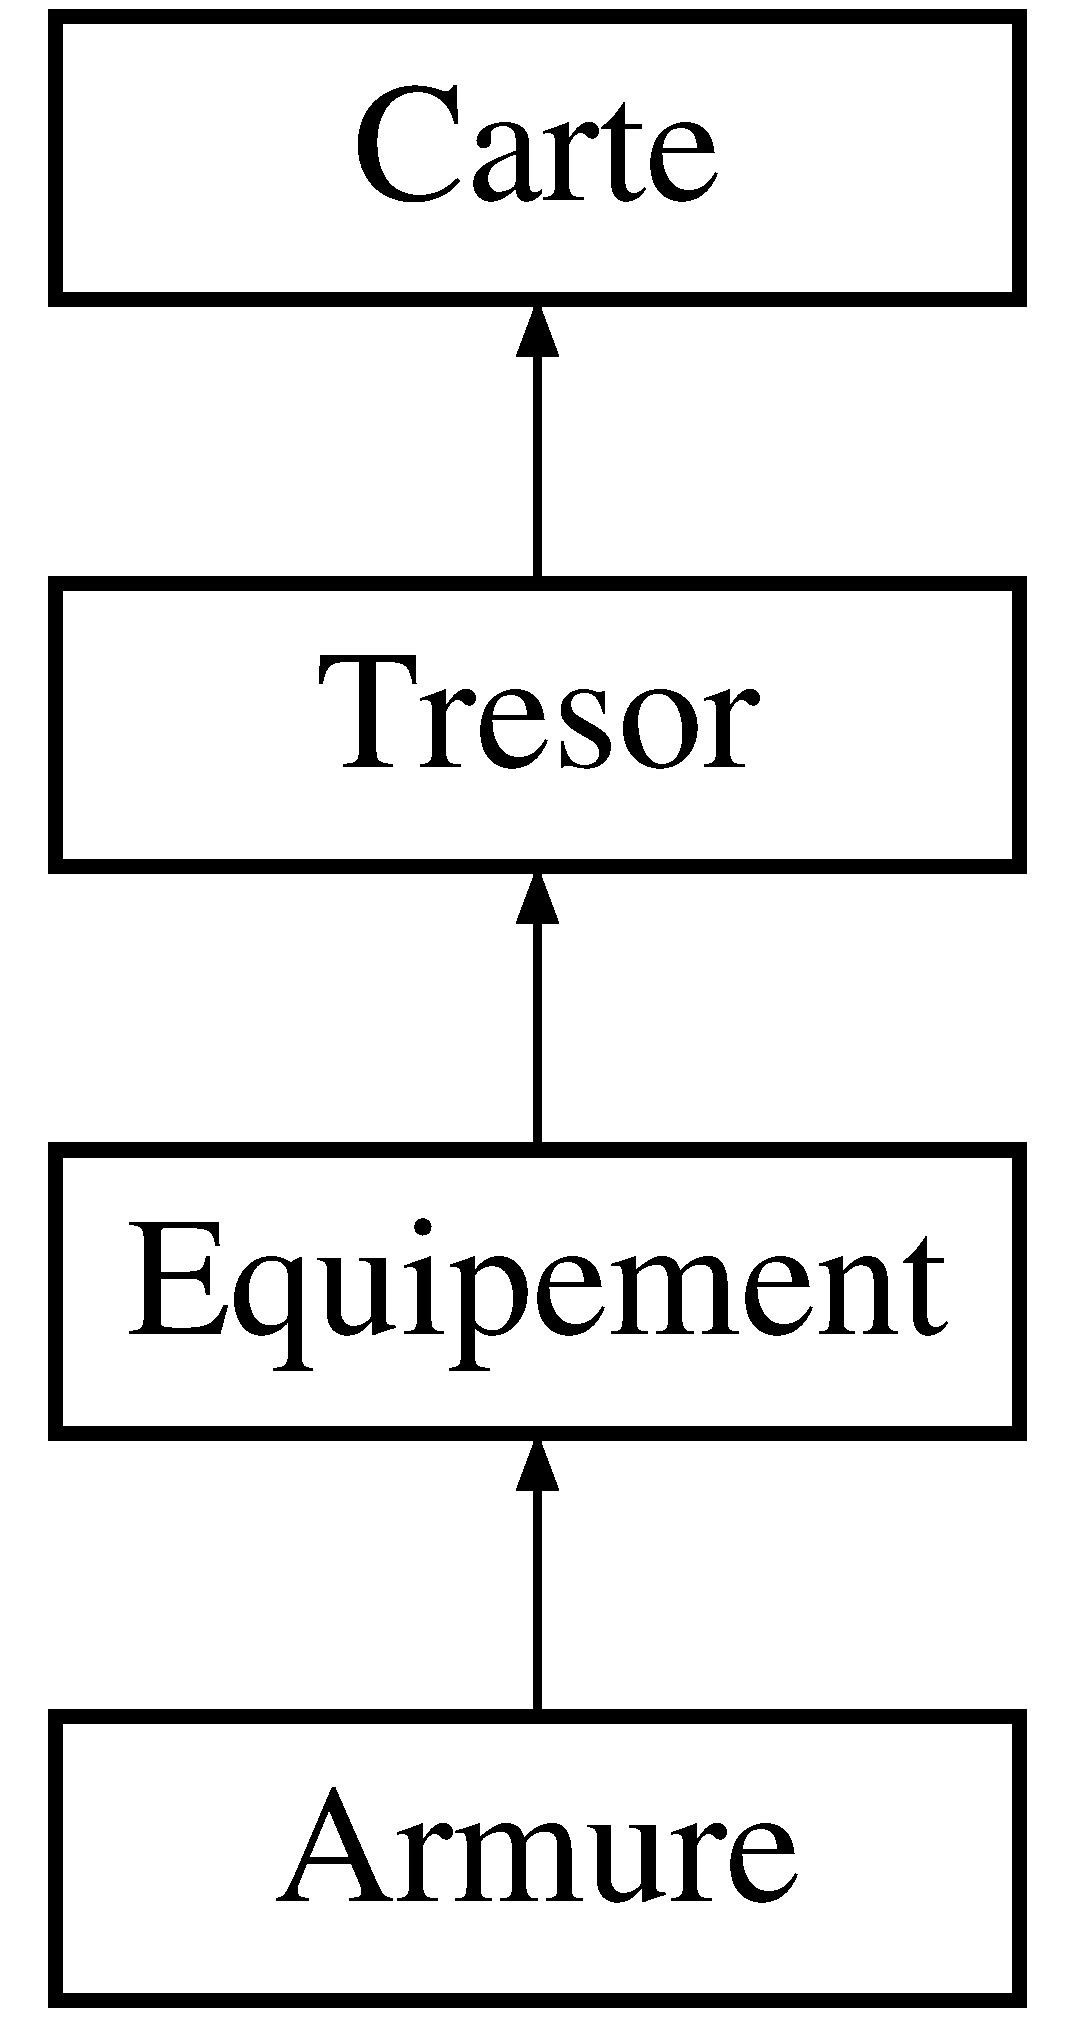
\includegraphics[height=4.000000cm]{class_armure}
\end{center}
\end{figure}
\subsection*{Public Member Functions}
\begin{DoxyCompactItemize}
\item 
\hyperlink{class_armure_ac26b4244239e19bebc5985064899bd4f}{Armure} (int id, std\-::string n, std\-::string d, int p)
\begin{DoxyCompactList}\small\item\em Constructeur de \hyperlink{class_armure}{Armure}. \end{DoxyCompactList}\item 
bool \hyperlink{class_armure_a5c0c3ffb5402e821b454076c5e3d99bc}{est\-Armure} ()
\begin{DoxyCompactList}\small\item\em Renvoie vrai si c'est une \hyperlink{class_armure}{Armure}. \end{DoxyCompactList}\end{DoxyCompactItemize}
\subsection*{Additional Inherited Members}


\subsection{Constructor \& Destructor Documentation}
\hypertarget{class_armure_ac26b4244239e19bebc5985064899bd4f}{\index{Armure@{Armure}!Armure@{Armure}}
\index{Armure@{Armure}!Armure@{Armure}}
\subsubsection[{Armure}]{\setlength{\rightskip}{0pt plus 5cm}Armure\-::\-Armure (
\begin{DoxyParamCaption}
\item[{int}]{id, }
\item[{std\-::string}]{n, }
\item[{std\-::string}]{d, }
\item[{int}]{p}
\end{DoxyParamCaption}
)}}\label{class_armure_ac26b4244239e19bebc5985064899bd4f}


Constructeur de \hyperlink{class_armure}{Armure}. 


\begin{DoxyParams}{Parameters}
{\em id} & Identifiant de la carte \\
\hline
{\em n} & nom de la carte \\
\hline
{\em d} & description de la carte \\
\hline
{\em p} & prix de la carte \\
\hline
\end{DoxyParams}


\subsection{Member Function Documentation}
\hypertarget{class_armure_a5c0c3ffb5402e821b454076c5e3d99bc}{\index{Armure@{Armure}!est\-Armure@{est\-Armure}}
\index{est\-Armure@{est\-Armure}!Armure@{Armure}}
\subsubsection[{est\-Armure}]{\setlength{\rightskip}{0pt plus 5cm}bool Armure\-::est\-Armure (
\begin{DoxyParamCaption}
{}
\end{DoxyParamCaption}
)\hspace{0.3cm}{\ttfamily [virtual]}}}\label{class_armure_a5c0c3ffb5402e821b454076c5e3d99bc}


Renvoie vrai si c'est une \hyperlink{class_armure}{Armure}. 

\begin{DoxyReturn}{Returns}
vrai si c'est une \hyperlink{class_armure}{Armure}, Faux sinon 
\end{DoxyReturn}


Reimplemented from \hyperlink{class_carte_a5d971af0574d33695afba7c525ef1a3e}{Carte}.



The documentation for this class was generated from the following files\-:\begin{DoxyCompactItemize}
\item 
\hyperlink{_armure_8hpp}{Armure.\-hpp}\item 
Armure.\-cpp\end{DoxyCompactItemize}

\hypertarget{class_attente}{\section{Attente Class Reference}
\label{class_attente}\index{Attente@{Attente}}
}
Inheritance diagram for Attente\-:\begin{figure}[H]
\begin{center}
\leavevmode
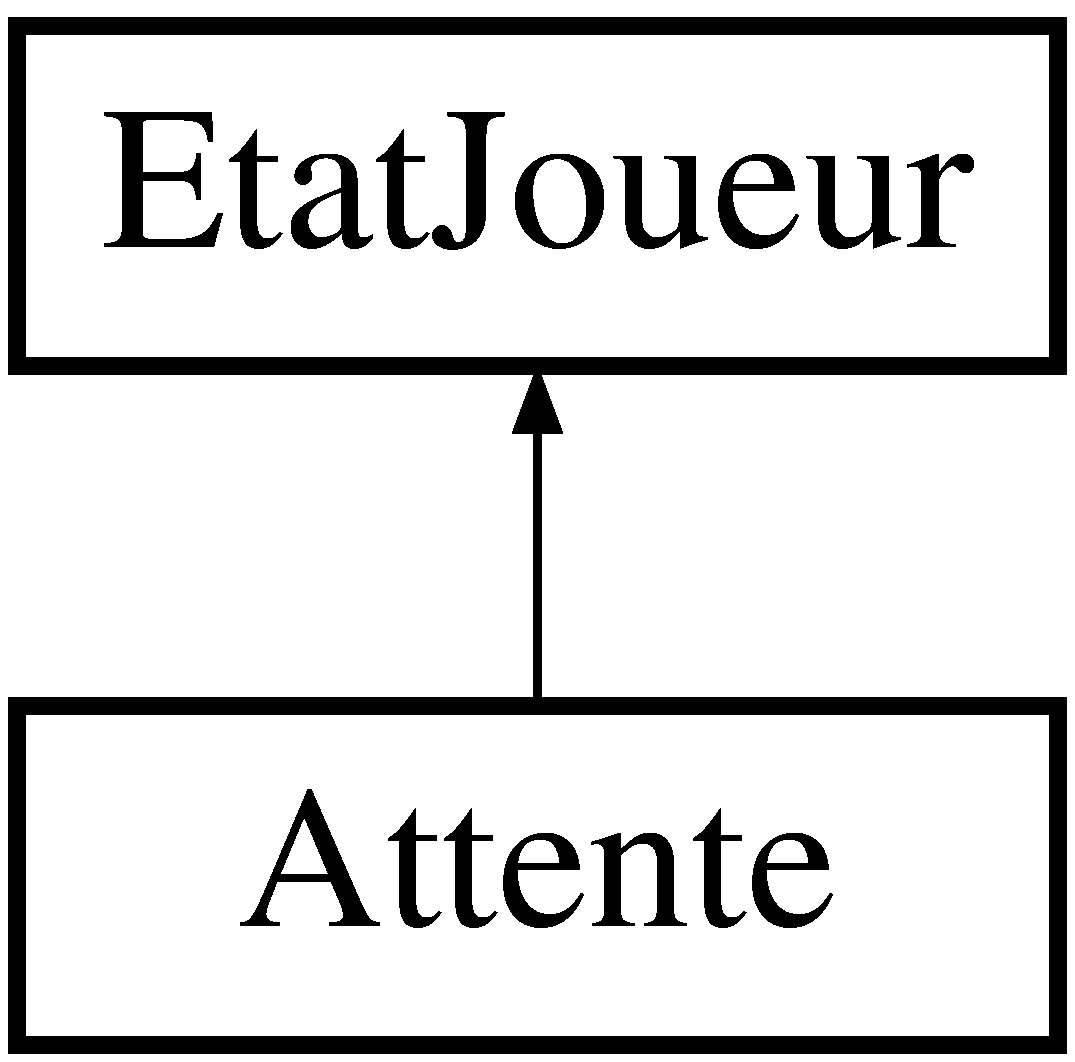
\includegraphics[height=2.000000cm]{class_attente}
\end{center}
\end{figure}
\subsection*{Public Member Functions}
\begin{DoxyCompactItemize}
\item 
\hyperlink{class_attente_a902ce251742271095c684b2808089527}{Attente} (\hyperlink{class_joueur}{Joueur} $\ast$t)
\begin{DoxyCompactList}\small\item\em Constructeur de \hyperlink{class_attente}{Attente}. \end{DoxyCompactList}\item 
\hypertarget{class_attente_ab0f2c48cf0f565521895ed7dc39add06}{virtual \hyperlink{class_attente_ab0f2c48cf0f565521895ed7dc39add06}{$\sim$\-Attente} ()}\label{class_attente_ab0f2c48cf0f565521895ed7dc39add06}

\begin{DoxyCompactList}\small\item\em Destructeur de \hyperlink{class_attente}{Attente}. \end{DoxyCompactList}\end{DoxyCompactItemize}
\subsection*{Additional Inherited Members}


\subsection{Constructor \& Destructor Documentation}
\hypertarget{class_attente_a902ce251742271095c684b2808089527}{\index{Attente@{Attente}!Attente@{Attente}}
\index{Attente@{Attente}!Attente@{Attente}}
\subsubsection[{Attente}]{\setlength{\rightskip}{0pt plus 5cm}Attente\-::\-Attente (
\begin{DoxyParamCaption}
\item[{{\bf Joueur} $\ast$}]{t}
\end{DoxyParamCaption}
)}}\label{class_attente_a902ce251742271095c684b2808089527}


Constructeur de \hyperlink{class_attente}{Attente}. 


\begin{DoxyParams}{Parameters}
{\em t} & \hyperlink{class_joueur}{Joueur} dont l'état doit être géré \\
\hline
\end{DoxyParams}


The documentation for this class was generated from the following files\-:\begin{DoxyCompactItemize}
\item 
\hyperlink{_attente_8hpp}{Attente.\-hpp}\item 
\hyperlink{_attente_8cpp}{Attente.\-cpp}\end{DoxyCompactItemize}

\hypertarget{class_bagarre}{\section{Bagarre Class Reference}
\label{class_bagarre}\index{Bagarre@{Bagarre}}
}
Inheritance diagram for Bagarre\-:\begin{figure}[H]
\begin{center}
\leavevmode
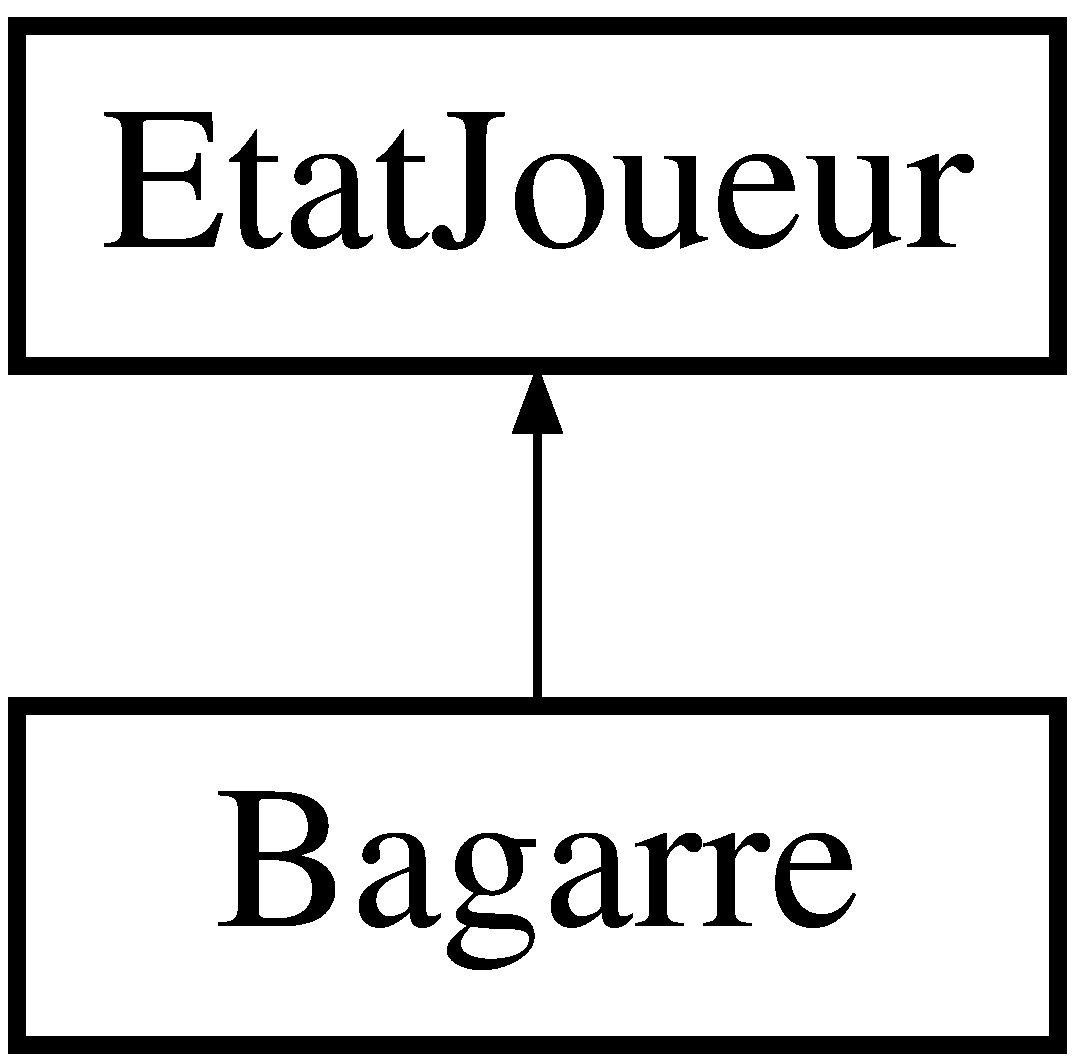
\includegraphics[height=2.000000cm]{class_bagarre}
\end{center}
\end{figure}
\subsection*{Public Member Functions}
\begin{DoxyCompactItemize}
\item 
\hyperlink{class_bagarre_acb7416e18dc7f862d416ccaf97c7e3e2}{Bagarre} (\hyperlink{class_joueur}{Joueur} $\ast$t)
\begin{DoxyCompactList}\small\item\em Constructeur de \hyperlink{class_bagarre}{Bagarre}. \end{DoxyCompactList}\item 
\hypertarget{class_bagarre_a4b37f229dd2b741cbfda7181e267b4f0}{virtual \hyperlink{class_bagarre_a4b37f229dd2b741cbfda7181e267b4f0}{$\sim$\-Bagarre} ()}\label{class_bagarre_a4b37f229dd2b741cbfda7181e267b4f0}

\begin{DoxyCompactList}\small\item\em Destructeur de \hyperlink{class_bagarre}{Bagarre}. \end{DoxyCompactList}\item 
void \hyperlink{class_bagarre_a084f695d366ea866270c2e8c5561c8fe}{combattre} (\hyperlink{class_carte}{Carte} $\ast$m)
\begin{DoxyCompactList}\small\item\em Permet au joueur de combattre un monstre. \end{DoxyCompactList}\item 
\hypertarget{class_bagarre_aae798fa4ff9eaaf30413f387302b1e3e}{void \hyperlink{class_bagarre_aae798fa4ff9eaaf30413f387302b1e3e}{deguerpir} ()}\label{class_bagarre_aae798fa4ff9eaaf30413f387302b1e3e}

\begin{DoxyCompactList}\small\item\em Permet au joueur de deguerpir lorsqu'il est en combat. \end{DoxyCompactList}\item 
void \hyperlink{class_bagarre_ae0a87f0398857acbabb9993886e96a82}{poser\-Potion} (\hyperlink{class_personnage}{Personnage} $\ast$p, \hyperlink{class_carte}{Carte} $\ast$po)
\begin{DoxyCompactList}\small\item\em Permet au joueur de poser une potion. \end{DoxyCompactList}\end{DoxyCompactItemize}
\subsection*{Additional Inherited Members}


\subsection{Constructor \& Destructor Documentation}
\hypertarget{class_bagarre_acb7416e18dc7f862d416ccaf97c7e3e2}{\index{Bagarre@{Bagarre}!Bagarre@{Bagarre}}
\index{Bagarre@{Bagarre}!Bagarre@{Bagarre}}
\subsubsection[{Bagarre}]{\setlength{\rightskip}{0pt plus 5cm}Bagarre\-::\-Bagarre (
\begin{DoxyParamCaption}
\item[{{\bf Joueur} $\ast$}]{t}
\end{DoxyParamCaption}
)}}\label{class_bagarre_acb7416e18dc7f862d416ccaf97c7e3e2}


Constructeur de \hyperlink{class_bagarre}{Bagarre}. 


\begin{DoxyParams}{Parameters}
{\em t} & \hyperlink{class_joueur}{Joueur} dont l'état doit être géré \\
\hline
\end{DoxyParams}


\subsection{Member Function Documentation}
\hypertarget{class_bagarre_a084f695d366ea866270c2e8c5561c8fe}{\index{Bagarre@{Bagarre}!combattre@{combattre}}
\index{combattre@{combattre}!Bagarre@{Bagarre}}
\subsubsection[{combattre}]{\setlength{\rightskip}{0pt plus 5cm}void Bagarre\-::combattre (
\begin{DoxyParamCaption}
\item[{{\bf Carte} $\ast$}]{m}
\end{DoxyParamCaption}
)\hspace{0.3cm}{\ttfamily [virtual]}}}\label{class_bagarre_a084f695d366ea866270c2e8c5561c8fe}


Permet au joueur de combattre un monstre. 


\begin{DoxyParams}{Parameters}
{\em m} & monstre à combattre \\
\hline
\end{DoxyParams}


Reimplemented from \hyperlink{class_etat_joueur_a63c672f1d599a82f88aa80aebedf78d6}{Etat\-Joueur}.

\hypertarget{class_bagarre_ae0a87f0398857acbabb9993886e96a82}{\index{Bagarre@{Bagarre}!poser\-Potion@{poser\-Potion}}
\index{poser\-Potion@{poser\-Potion}!Bagarre@{Bagarre}}
\subsubsection[{poser\-Potion}]{\setlength{\rightskip}{0pt plus 5cm}void Bagarre\-::poser\-Potion (
\begin{DoxyParamCaption}
\item[{{\bf Personnage} $\ast$}]{p, }
\item[{{\bf Carte} $\ast$}]{po}
\end{DoxyParamCaption}
)\hspace{0.3cm}{\ttfamily [virtual]}}}\label{class_bagarre_ae0a87f0398857acbabb9993886e96a82}


Permet au joueur de poser une potion. 


\begin{DoxyParams}{Parameters}
{\em cible} & cible de la potion \\
\hline
{\em po} & potion à poser \\
\hline
\end{DoxyParams}


Reimplemented from \hyperlink{class_etat_joueur_a76cf1ff3d4140f182a07167a5053f509}{Etat\-Joueur}.



The documentation for this class was generated from the following files\-:\begin{DoxyCompactItemize}
\item 
\hyperlink{_bagarre_8hpp}{Bagarre.\-hpp}\item 
\hyperlink{_bagarre_8cpp}{Bagarre.\-cpp}\end{DoxyCompactItemize}

\hypertarget{class_carte}{\section{Carte Class Reference}
\label{class_carte}\index{Carte@{Carte}}
}
Inheritance diagram for Carte\-:\begin{figure}[H]
\begin{center}
\leavevmode
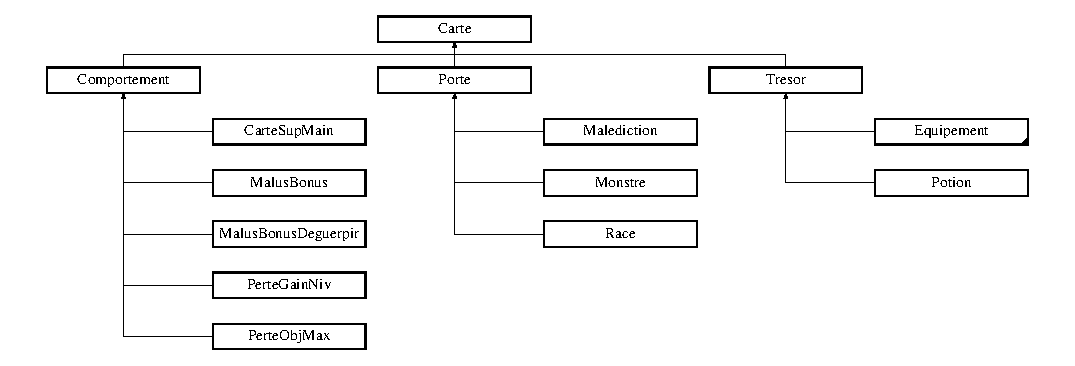
\includegraphics[height=4.474886cm]{class_carte}
\end{center}
\end{figure}
\subsection*{Public Member Functions}
\begin{DoxyCompactItemize}
\item 
\hyperlink{class_carte_a85f142caee17cf2531dfff69490958b4}{Carte} (int id, std\-::string n, std\-::string d)
\begin{DoxyCompactList}\small\item\em Constructeur de carte. \end{DoxyCompactList}\item 
\hypertarget{class_carte_a63300ff55c58b5d5b1674a3fc8f25910}{virtual \hyperlink{class_carte_a63300ff55c58b5d5b1674a3fc8f25910}{$\sim$\-Carte} ()}\label{class_carte_a63300ff55c58b5d5b1674a3fc8f25910}

\begin{DoxyCompactList}\small\item\em Destructeur de carte. \end{DoxyCompactList}\item 
virtual std\-::string \hyperlink{class_carte_a7b68885ddbd8c8f6991e5447346913bc}{get\-Nom} ()
\begin{DoxyCompactList}\small\item\em Renvoie le nom de la carte. \end{DoxyCompactList}\item 
virtual std\-::string \hyperlink{class_carte_a591705d6bb95c36ce4a034b3107ae85c}{get\-Description} ()
\begin{DoxyCompactList}\small\item\em Renvoie la description de la carte. \end{DoxyCompactList}\item 
virtual \hyperlink{class_carte}{Carte} $\ast$ \hyperlink{class_carte_a03711d12e3252863aa4303b3edc5c118}{get\-Carte} ()
\begin{DoxyCompactList}\small\item\em Renvoie un pointeur sur cet �l�ment. \end{DoxyCompactList}\item 
virtual bool \hyperlink{class_carte_af0156ad1b4b87414df65caddd310212a}{est\-Porte} ()
\begin{DoxyCompactList}\small\item\em Renvoie vrai si c'est une \hyperlink{class_porte}{Porte}. \end{DoxyCompactList}\item 
virtual bool \hyperlink{class_carte_af9c84ec45b9a570d8ac8019726756ee7}{est\-Malediction} ()
\begin{DoxyCompactList}\small\item\em Renvoie vrai si c'est une \hyperlink{class_malediction}{Malediction}. \end{DoxyCompactList}\item 
virtual bool \hyperlink{class_carte_a74c9bf2967ea099015d1b96003f9da18}{est\-Monstre} ()
\begin{DoxyCompactList}\small\item\em Renvoie vrai si c'est un \hyperlink{class_monstre}{Monstre}. \end{DoxyCompactList}\item 
virtual bool \hyperlink{class_carte_acbac53716e6285801ca151aa177fc699}{est\-Race} ()
\begin{DoxyCompactList}\small\item\em Renvoie vrai si c'est une \hyperlink{class_race}{Race}. \end{DoxyCompactList}\item 
virtual bool \hyperlink{class_carte_a3be68ed1ee99d835cd27148e456e5b9c}{est\-Potion} ()
\begin{DoxyCompactList}\small\item\em Renvoie vrai si c'est une \hyperlink{class_potion}{Potion}. \end{DoxyCompactList}\item 
virtual bool \hyperlink{class_carte_abcf22b28f170502cb4f17f2c0b7a031f}{est\-Equipement} ()
\begin{DoxyCompactList}\small\item\em Renvoie vrai si c'est un \hyperlink{class_equipement}{Equipement}. \end{DoxyCompactList}\item 
virtual bool \hyperlink{class_carte_a5d971af0574d33695afba7c525ef1a3e}{est\-Armure} ()
\begin{DoxyCompactList}\small\item\em Renvoie vrai si c'est une \hyperlink{class_armure}{Armure}. \end{DoxyCompactList}\item 
virtual bool \hyperlink{class_carte_a830cd4aac4b93fab69a0901d35e562ab}{est\-Chaussure} ()
\begin{DoxyCompactList}\small\item\em Renvoie vrai si c'est une \hyperlink{class_chaussure}{Chaussure}. \end{DoxyCompactList}\item 
virtual bool \hyperlink{class_carte_aeb1c07fe1a7071b2d6d4a14bbeb032f5}{est\-Couvre\-Chef} ()
\begin{DoxyCompactList}\small\item\em Renvoie vrai si c'est un \hyperlink{class_couvre_chef}{Couvre\-Chef}. \end{DoxyCompactList}\item 
virtual bool \hyperlink{class_carte_a13cfbbcd63cd11659ada554db42f6a3f}{est\-Main} ()
\begin{DoxyCompactList}\small\item\em Renvoie vrai si c'est une \hyperlink{class_main}{Main}. \end{DoxyCompactList}\item 
virtual bool \hyperlink{class_carte_a5fcbed672fcb0141ac2349db64d82385}{est\-Tresor} ()
\begin{DoxyCompactList}\small\item\em Renvoie vrai si c'est une \hyperlink{class_tresor}{Tresor}. \end{DoxyCompactList}\item 
virtual void \hyperlink{class_carte_ade8947dac978d46922ccff92aebf54f7}{appliquer} (\hyperlink{class_personnage}{Personnage} $\ast$p)
\begin{DoxyCompactList}\small\item\em applique le comportement de la carte \end{DoxyCompactList}\item 
virtual void \hyperlink{class_carte_a938f4d4a1df46c4fc695c01e4bf585ba}{retirer} (\hyperlink{class_personnage}{Personnage} $\ast$p)
\begin{DoxyCompactList}\small\item\em retire le comportement de la carte \end{DoxyCompactList}\item 
virtual int \hyperlink{class_carte_ada584f087ef345e6ebf7955be74c4084}{get\-Valeur} ()
\begin{DoxyCompactList}\small\item\em renvoie la valeur du comportement \end{DoxyCompactList}\item 
int \hyperlink{class_carte_ae51a40df8fb2ab5498ae67e165ceb5f2}{get\-Id} ()
\begin{DoxyCompactList}\small\item\em renvoie l'identifiant \end{DoxyCompactList}\item 
bool \hyperlink{class_carte_a5fd7084b52e3c47e830ba319b402782e}{compare} (\hyperlink{class_carte}{Carte} $\ast$e)
\begin{DoxyCompactList}\small\item\em Permet de comparer 2 cartes. \end{DoxyCompactList}\end{DoxyCompactItemize}
\subsection*{Protected Attributes}
\begin{DoxyCompactItemize}
\item 
int \hyperlink{class_carte_aafef265451f5c4c38ec27f8f53ae4509}{identifiant}
\item 
std\-::string \hyperlink{class_carte_a46bff2b84b76b6b94b2eaa3fe813ec69}{nom}
\item 
std\-::string \hyperlink{class_carte_a5f2acc07fa281fb6d4467c00bd4b1614}{description}
\end{DoxyCompactItemize}


\subsection{Constructor \& Destructor Documentation}
\hypertarget{class_carte_a85f142caee17cf2531dfff69490958b4}{\index{Carte@{Carte}!Carte@{Carte}}
\index{Carte@{Carte}!Carte@{Carte}}
\subsubsection[{Carte}]{\setlength{\rightskip}{0pt plus 5cm}Carte\-::\-Carte (
\begin{DoxyParamCaption}
\item[{int}]{id, }
\item[{std\-::string}]{n, }
\item[{std\-::string}]{d}
\end{DoxyParamCaption}
)}}\label{class_carte_a85f142caee17cf2531dfff69490958b4}


Constructeur de carte. 


\begin{DoxyParams}{Parameters}
{\em id} & Identifiant de la carte \\
\hline
{\em n} & nom de la carte \\
\hline
{\em d} & description de la carte \\
\hline
\end{DoxyParams}


\subsection{Member Function Documentation}
\hypertarget{class_carte_ade8947dac978d46922ccff92aebf54f7}{\index{Carte@{Carte}!appliquer@{appliquer}}
\index{appliquer@{appliquer}!Carte@{Carte}}
\subsubsection[{appliquer}]{\setlength{\rightskip}{0pt plus 5cm}void Carte\-::appliquer (
\begin{DoxyParamCaption}
\item[{{\bf Personnage} $\ast$}]{p}
\end{DoxyParamCaption}
)\hspace{0.3cm}{\ttfamily [virtual]}}}\label{class_carte_ade8947dac978d46922ccff92aebf54f7}


applique le comportement de la carte 


\begin{DoxyParams}{Parameters}
{\em cible} & du comportement \\
\hline
\end{DoxyParams}


Reimplemented in \hyperlink{class_comportement_ae55149d29c710b0a5a0388cae308024f}{Comportement}, \hyperlink{class_carte_sup_main_adc7d3cf6f6e126400abad30e874cb24e}{Carte\-Sup\-Main}, \hyperlink{class_malus_bonus_aede2c45aa2a0d0f751c128e05d26fb6a}{Malus\-Bonus}, \hyperlink{class_malus_bonus_deguerpir_a703620e87d5d861ba850a3b07f61195a}{Malus\-Bonus\-Deguerpir}, \hyperlink{class_perte_gain_niv_ad72efe1c526391084768a500bb1ae4fa}{Perte\-Gain\-Niv}, and \hyperlink{class_perte_obj_max_a929e1c6370247feb937ae1835648a441}{Perte\-Obj\-Max}.

\hypertarget{class_carte_a5fd7084b52e3c47e830ba319b402782e}{\index{Carte@{Carte}!compare@{compare}}
\index{compare@{compare}!Carte@{Carte}}
\subsubsection[{compare}]{\setlength{\rightskip}{0pt plus 5cm}bool Carte\-::compare (
\begin{DoxyParamCaption}
\item[{{\bf Carte} $\ast$}]{e}
\end{DoxyParamCaption}
)}}\label{class_carte_a5fd7084b52e3c47e830ba319b402782e}


Permet de comparer 2 cartes. 


\begin{DoxyParams}{Parameters}
{\em \hyperlink{class_carte}{Carte}} & � comparer avec this \\
\hline
\end{DoxyParams}
\begin{DoxyReturn}{Returns}
Vrai si elles ont le m�me nom, faux sinon 
\end{DoxyReturn}
\hypertarget{class_carte_a5d971af0574d33695afba7c525ef1a3e}{\index{Carte@{Carte}!est\-Armure@{est\-Armure}}
\index{est\-Armure@{est\-Armure}!Carte@{Carte}}
\subsubsection[{est\-Armure}]{\setlength{\rightskip}{0pt plus 5cm}bool Carte\-::est\-Armure (
\begin{DoxyParamCaption}
{}
\end{DoxyParamCaption}
)\hspace{0.3cm}{\ttfamily [virtual]}}}\label{class_carte_a5d971af0574d33695afba7c525ef1a3e}


Renvoie vrai si c'est une \hyperlink{class_armure}{Armure}. 

\begin{DoxyReturn}{Returns}
vrai si c'est une \hyperlink{class_armure}{Armure}, Faux sinon 
\end{DoxyReturn}


Reimplemented in \hyperlink{class_comportement_a3fc939a96fbe4154af5b104ecc7a1afd}{Comportement}, and \hyperlink{class_armure_a5c0c3ffb5402e821b454076c5e3d99bc}{Armure}.

\hypertarget{class_carte_a830cd4aac4b93fab69a0901d35e562ab}{\index{Carte@{Carte}!est\-Chaussure@{est\-Chaussure}}
\index{est\-Chaussure@{est\-Chaussure}!Carte@{Carte}}
\subsubsection[{est\-Chaussure}]{\setlength{\rightskip}{0pt plus 5cm}bool Carte\-::est\-Chaussure (
\begin{DoxyParamCaption}
{}
\end{DoxyParamCaption}
)\hspace{0.3cm}{\ttfamily [virtual]}}}\label{class_carte_a830cd4aac4b93fab69a0901d35e562ab}


Renvoie vrai si c'est une \hyperlink{class_chaussure}{Chaussure}. 

\begin{DoxyReturn}{Returns}
vrai si c'est une \hyperlink{class_chaussure}{Chaussure}, Faux sinon 
\end{DoxyReturn}


Reimplemented in \hyperlink{class_comportement_ab862b3685bf0f29f204ea96b98dc1d4b}{Comportement}, and \hyperlink{class_chaussure_a1d9c1abb1dc4c3bd6476fa19a5885973}{Chaussure}.

\hypertarget{class_carte_aeb1c07fe1a7071b2d6d4a14bbeb032f5}{\index{Carte@{Carte}!est\-Couvre\-Chef@{est\-Couvre\-Chef}}
\index{est\-Couvre\-Chef@{est\-Couvre\-Chef}!Carte@{Carte}}
\subsubsection[{est\-Couvre\-Chef}]{\setlength{\rightskip}{0pt plus 5cm}bool Carte\-::est\-Couvre\-Chef (
\begin{DoxyParamCaption}
{}
\end{DoxyParamCaption}
)\hspace{0.3cm}{\ttfamily [virtual]}}}\label{class_carte_aeb1c07fe1a7071b2d6d4a14bbeb032f5}


Renvoie vrai si c'est un \hyperlink{class_couvre_chef}{Couvre\-Chef}. 

\begin{DoxyReturn}{Returns}
vrai si c'est un \hyperlink{class_couvre_chef}{Couvre\-Chef}, Faux sinon 
\end{DoxyReturn}


Reimplemented in \hyperlink{class_comportement_ae3b252fd5bd95df0d2cdfab1242db808}{Comportement}, and \hyperlink{class_couvre_chef_a1fab97ed5b18d67c5dd40f5fa49c1a02}{Couvre\-Chef}.

\hypertarget{class_carte_abcf22b28f170502cb4f17f2c0b7a031f}{\index{Carte@{Carte}!est\-Equipement@{est\-Equipement}}
\index{est\-Equipement@{est\-Equipement}!Carte@{Carte}}
\subsubsection[{est\-Equipement}]{\setlength{\rightskip}{0pt plus 5cm}bool Carte\-::est\-Equipement (
\begin{DoxyParamCaption}
{}
\end{DoxyParamCaption}
)\hspace{0.3cm}{\ttfamily [virtual]}}}\label{class_carte_abcf22b28f170502cb4f17f2c0b7a031f}


Renvoie vrai si c'est un \hyperlink{class_equipement}{Equipement}. 

\begin{DoxyReturn}{Returns}
vrai si c'est une \hyperlink{class_equipement}{Equipement}, Faux sinon 
\end{DoxyReturn}


Reimplemented in \hyperlink{class_comportement_aae304a510ec6096fcb4337a72f0fcd72}{Comportement}, and \hyperlink{class_equipement_ab720166d5e8dd681224de3d9490c106d}{Equipement}.

\hypertarget{class_carte_a13cfbbcd63cd11659ada554db42f6a3f}{\index{Carte@{Carte}!est\-Main@{est\-Main}}
\index{est\-Main@{est\-Main}!Carte@{Carte}}
\subsubsection[{est\-Main}]{\setlength{\rightskip}{0pt plus 5cm}bool Carte\-::est\-Main (
\begin{DoxyParamCaption}
{}
\end{DoxyParamCaption}
)\hspace{0.3cm}{\ttfamily [virtual]}}}\label{class_carte_a13cfbbcd63cd11659ada554db42f6a3f}


Renvoie vrai si c'est une \hyperlink{class_main}{Main}. 

\begin{DoxyReturn}{Returns}
vrai si c'est une \hyperlink{class_main}{Main}, Faux sinon 
\end{DoxyReturn}


Reimplemented in \hyperlink{class_comportement_a91ac9d0063ac95f333ab62f5034cc3ce}{Comportement}, and \hyperlink{class_main_aba193ef84e793b04254c1a13031a0c92}{Main}.

\hypertarget{class_carte_af9c84ec45b9a570d8ac8019726756ee7}{\index{Carte@{Carte}!est\-Malediction@{est\-Malediction}}
\index{est\-Malediction@{est\-Malediction}!Carte@{Carte}}
\subsubsection[{est\-Malediction}]{\setlength{\rightskip}{0pt plus 5cm}bool Carte\-::est\-Malediction (
\begin{DoxyParamCaption}
{}
\end{DoxyParamCaption}
)\hspace{0.3cm}{\ttfamily [virtual]}}}\label{class_carte_af9c84ec45b9a570d8ac8019726756ee7}


Renvoie vrai si c'est une \hyperlink{class_malediction}{Malediction}. 

\begin{DoxyReturn}{Returns}
vrai si c'est une \hyperlink{class_malediction}{Malediction}, Faux sinon 
\end{DoxyReturn}


Reimplemented in \hyperlink{class_comportement_a7598241705f53e86b1d08dce11a1a4dd}{Comportement}, and \hyperlink{class_malediction_a3e374642e5326239e9d613bd2233c1be}{Malediction}.

\hypertarget{class_carte_a74c9bf2967ea099015d1b96003f9da18}{\index{Carte@{Carte}!est\-Monstre@{est\-Monstre}}
\index{est\-Monstre@{est\-Monstre}!Carte@{Carte}}
\subsubsection[{est\-Monstre}]{\setlength{\rightskip}{0pt plus 5cm}bool Carte\-::est\-Monstre (
\begin{DoxyParamCaption}
{}
\end{DoxyParamCaption}
)\hspace{0.3cm}{\ttfamily [virtual]}}}\label{class_carte_a74c9bf2967ea099015d1b96003f9da18}


Renvoie vrai si c'est un \hyperlink{class_monstre}{Monstre}. 

\begin{DoxyReturn}{Returns}
vrai si c'est un \hyperlink{class_monstre}{Monstre}, Faux sinon 
\end{DoxyReturn}


Reimplemented in \hyperlink{class_comportement_a8cfc80bb17c61c7e5597c50609ec2cfe}{Comportement}, and \hyperlink{class_monstre_ad01432b5c676e4607e550d4c5595d5ea}{Monstre}.

\hypertarget{class_carte_af0156ad1b4b87414df65caddd310212a}{\index{Carte@{Carte}!est\-Porte@{est\-Porte}}
\index{est\-Porte@{est\-Porte}!Carte@{Carte}}
\subsubsection[{est\-Porte}]{\setlength{\rightskip}{0pt plus 5cm}bool Carte\-::est\-Porte (
\begin{DoxyParamCaption}
{}
\end{DoxyParamCaption}
)\hspace{0.3cm}{\ttfamily [virtual]}}}\label{class_carte_af0156ad1b4b87414df65caddd310212a}


Renvoie vrai si c'est une \hyperlink{class_porte}{Porte}. 

\begin{DoxyReturn}{Returns}
vrai si c'est une \hyperlink{class_porte}{Porte}, Faux sinon 
\end{DoxyReturn}


Reimplemented in \hyperlink{class_comportement_a25ae445c0424638fd2eef12123960d4b}{Comportement}, and \hyperlink{class_porte_a8a7e6c7c6b1d94b157b2229a6e32ac93}{Porte}.

\hypertarget{class_carte_a3be68ed1ee99d835cd27148e456e5b9c}{\index{Carte@{Carte}!est\-Potion@{est\-Potion}}
\index{est\-Potion@{est\-Potion}!Carte@{Carte}}
\subsubsection[{est\-Potion}]{\setlength{\rightskip}{0pt plus 5cm}bool Carte\-::est\-Potion (
\begin{DoxyParamCaption}
{}
\end{DoxyParamCaption}
)\hspace{0.3cm}{\ttfamily [virtual]}}}\label{class_carte_a3be68ed1ee99d835cd27148e456e5b9c}


Renvoie vrai si c'est une \hyperlink{class_potion}{Potion}. 

\begin{DoxyReturn}{Returns}
vrai si c'est une \hyperlink{class_potion}{Potion}, Faux sinon 
\end{DoxyReturn}


Reimplemented in \hyperlink{class_comportement_a2bd892e21d3f14e5e585be037d6ec5bd}{Comportement}, and \hyperlink{class_potion_aa04fc4873583e7b1f90416b226edbe06}{Potion}.

\hypertarget{class_carte_acbac53716e6285801ca151aa177fc699}{\index{Carte@{Carte}!est\-Race@{est\-Race}}
\index{est\-Race@{est\-Race}!Carte@{Carte}}
\subsubsection[{est\-Race}]{\setlength{\rightskip}{0pt plus 5cm}bool Carte\-::est\-Race (
\begin{DoxyParamCaption}
{}
\end{DoxyParamCaption}
)\hspace{0.3cm}{\ttfamily [virtual]}}}\label{class_carte_acbac53716e6285801ca151aa177fc699}


Renvoie vrai si c'est une \hyperlink{class_race}{Race}. 

\begin{DoxyReturn}{Returns}
vrai si c'est une \hyperlink{class_race}{Race}, Faux sinon 
\end{DoxyReturn}


Reimplemented in \hyperlink{class_comportement_a0aaa6b86b322e54ff2d0c1e448a650c4}{Comportement}, and \hyperlink{class_race_a4d583fa670a0c3666715b89f86935060}{Race}.

\hypertarget{class_carte_a5fcbed672fcb0141ac2349db64d82385}{\index{Carte@{Carte}!est\-Tresor@{est\-Tresor}}
\index{est\-Tresor@{est\-Tresor}!Carte@{Carte}}
\subsubsection[{est\-Tresor}]{\setlength{\rightskip}{0pt plus 5cm}bool Carte\-::est\-Tresor (
\begin{DoxyParamCaption}
{}
\end{DoxyParamCaption}
)\hspace{0.3cm}{\ttfamily [virtual]}}}\label{class_carte_a5fcbed672fcb0141ac2349db64d82385}


Renvoie vrai si c'est une \hyperlink{class_tresor}{Tresor}. 

\begin{DoxyReturn}{Returns}
vrai si c'est un tr�sor, Faux sinon 
\end{DoxyReturn}


Reimplemented in \hyperlink{class_tresor_ade57ffa16e80824293ca128f18b9c648}{Tresor}.

\hypertarget{class_carte_a03711d12e3252863aa4303b3edc5c118}{\index{Carte@{Carte}!get\-Carte@{get\-Carte}}
\index{get\-Carte@{get\-Carte}!Carte@{Carte}}
\subsubsection[{get\-Carte}]{\setlength{\rightskip}{0pt plus 5cm}{\bf Carte} $\ast$ Carte\-::get\-Carte (
\begin{DoxyParamCaption}
{}
\end{DoxyParamCaption}
)\hspace{0.3cm}{\ttfamily [virtual]}}}\label{class_carte_a03711d12e3252863aa4303b3edc5c118}


Renvoie un pointeur sur cet �l�ment. 

\begin{DoxyReturn}{Returns}
pointeur sur cet �l�ment 
\end{DoxyReturn}


Reimplemented in \hyperlink{class_comportement_ae05651b07ef8145ae070507ea455241c}{Comportement}.

\hypertarget{class_carte_a591705d6bb95c36ce4a034b3107ae85c}{\index{Carte@{Carte}!get\-Description@{get\-Description}}
\index{get\-Description@{get\-Description}!Carte@{Carte}}
\subsubsection[{get\-Description}]{\setlength{\rightskip}{0pt plus 5cm}std\-::string Carte\-::get\-Description (
\begin{DoxyParamCaption}
{}
\end{DoxyParamCaption}
)\hspace{0.3cm}{\ttfamily [virtual]}}}\label{class_carte_a591705d6bb95c36ce4a034b3107ae85c}


Renvoie la description de la carte. 

\begin{DoxyReturn}{Returns}
description de la carte 
\end{DoxyReturn}


Reimplemented in \hyperlink{class_comportement_a534918dd72e2e3c1d2ecbd85f1c38e65}{Comportement}.

\hypertarget{class_carte_ae51a40df8fb2ab5498ae67e165ceb5f2}{\index{Carte@{Carte}!get\-Id@{get\-Id}}
\index{get\-Id@{get\-Id}!Carte@{Carte}}
\subsubsection[{get\-Id}]{\setlength{\rightskip}{0pt plus 5cm}int Carte\-::get\-Id (
\begin{DoxyParamCaption}
{}
\end{DoxyParamCaption}
)}}\label{class_carte_ae51a40df8fb2ab5498ae67e165ceb5f2}


renvoie l'identifiant 

\begin{DoxyReturn}{Returns}
la valeur de l'identifiant 
\end{DoxyReturn}
\hypertarget{class_carte_a7b68885ddbd8c8f6991e5447346913bc}{\index{Carte@{Carte}!get\-Nom@{get\-Nom}}
\index{get\-Nom@{get\-Nom}!Carte@{Carte}}
\subsubsection[{get\-Nom}]{\setlength{\rightskip}{0pt plus 5cm}std\-::string Carte\-::get\-Nom (
\begin{DoxyParamCaption}
{}
\end{DoxyParamCaption}
)\hspace{0.3cm}{\ttfamily [virtual]}}}\label{class_carte_a7b68885ddbd8c8f6991e5447346913bc}


Renvoie le nom de la carte. 

\begin{DoxyReturn}{Returns}
nom de la carte 
\end{DoxyReturn}


Reimplemented in \hyperlink{class_comportement_a0dd697e029b781d83f3251204845530e}{Comportement}.

\hypertarget{class_carte_ada584f087ef345e6ebf7955be74c4084}{\index{Carte@{Carte}!get\-Valeur@{get\-Valeur}}
\index{get\-Valeur@{get\-Valeur}!Carte@{Carte}}
\subsubsection[{get\-Valeur}]{\setlength{\rightskip}{0pt plus 5cm}int Carte\-::get\-Valeur (
\begin{DoxyParamCaption}
{}
\end{DoxyParamCaption}
)\hspace{0.3cm}{\ttfamily [virtual]}}}\label{class_carte_ada584f087ef345e6ebf7955be74c4084}


renvoie la valeur du comportement 

\begin{DoxyReturn}{Returns}
la valeur du comportement 
\end{DoxyReturn}


Reimplemented in \hyperlink{class_comportement_a0aa55aa40f00b6e9a2775126e39f0de7}{Comportement}.

\hypertarget{class_carte_a938f4d4a1df46c4fc695c01e4bf585ba}{\index{Carte@{Carte}!retirer@{retirer}}
\index{retirer@{retirer}!Carte@{Carte}}
\subsubsection[{retirer}]{\setlength{\rightskip}{0pt plus 5cm}void Carte\-::retirer (
\begin{DoxyParamCaption}
\item[{{\bf Personnage} $\ast$}]{p}
\end{DoxyParamCaption}
)\hspace{0.3cm}{\ttfamily [virtual]}}}\label{class_carte_a938f4d4a1df46c4fc695c01e4bf585ba}


retire le comportement de la carte 


\begin{DoxyParams}{Parameters}
{\em cible} & du comportement \\
\hline
\end{DoxyParams}


Reimplemented in \hyperlink{class_comportement_a7be9c46a6ae6d49ca3f49288b438b689}{Comportement}, \hyperlink{class_carte_sup_main_aa2b63cb5ea72b186931bbd8f093d9e20}{Carte\-Sup\-Main}, \hyperlink{class_malus_bonus_a213a8e9301ac84e2cf338476bf6613fc}{Malus\-Bonus}, and \hyperlink{class_malus_bonus_deguerpir_af7889dc668d138990d4e255c76bb8a89}{Malus\-Bonus\-Deguerpir}.



\subsection{Member Data Documentation}
\hypertarget{class_carte_a5f2acc07fa281fb6d4467c00bd4b1614}{\index{Carte@{Carte}!description@{description}}
\index{description@{description}!Carte@{Carte}}
\subsubsection[{description}]{\setlength{\rightskip}{0pt plus 5cm}std\-::string Carte\-::description\hspace{0.3cm}{\ttfamily [protected]}}}\label{class_carte_a5f2acc07fa281fb6d4467c00bd4b1614}
description de la carte \hypertarget{class_carte_aafef265451f5c4c38ec27f8f53ae4509}{\index{Carte@{Carte}!identifiant@{identifiant}}
\index{identifiant@{identifiant}!Carte@{Carte}}
\subsubsection[{identifiant}]{\setlength{\rightskip}{0pt plus 5cm}int Carte\-::identifiant\hspace{0.3cm}{\ttfamily [protected]}}}\label{class_carte_aafef265451f5c4c38ec27f8f53ae4509}
identifient de la carte \hypertarget{class_carte_a46bff2b84b76b6b94b2eaa3fe813ec69}{\index{Carte@{Carte}!nom@{nom}}
\index{nom@{nom}!Carte@{Carte}}
\subsubsection[{nom}]{\setlength{\rightskip}{0pt plus 5cm}std\-::string Carte\-::nom\hspace{0.3cm}{\ttfamily [protected]}}}\label{class_carte_a46bff2b84b76b6b94b2eaa3fe813ec69}
nom de la carte 

The documentation for this class was generated from the following files\-:\begin{DoxyCompactItemize}
\item 
\hyperlink{_carte_8hpp}{Carte.\-hpp}\item 
\hyperlink{_carte_8cpp}{Carte.\-cpp}\end{DoxyCompactItemize}

\hypertarget{class_carte_sup_main}{\section{Carte\-Sup\-Main Class Reference}
\label{class_carte_sup_main}\index{Carte\-Sup\-Main@{Carte\-Sup\-Main}}
}
Inheritance diagram for Carte\-Sup\-Main\-:\begin{figure}[H]
\begin{center}
\leavevmode
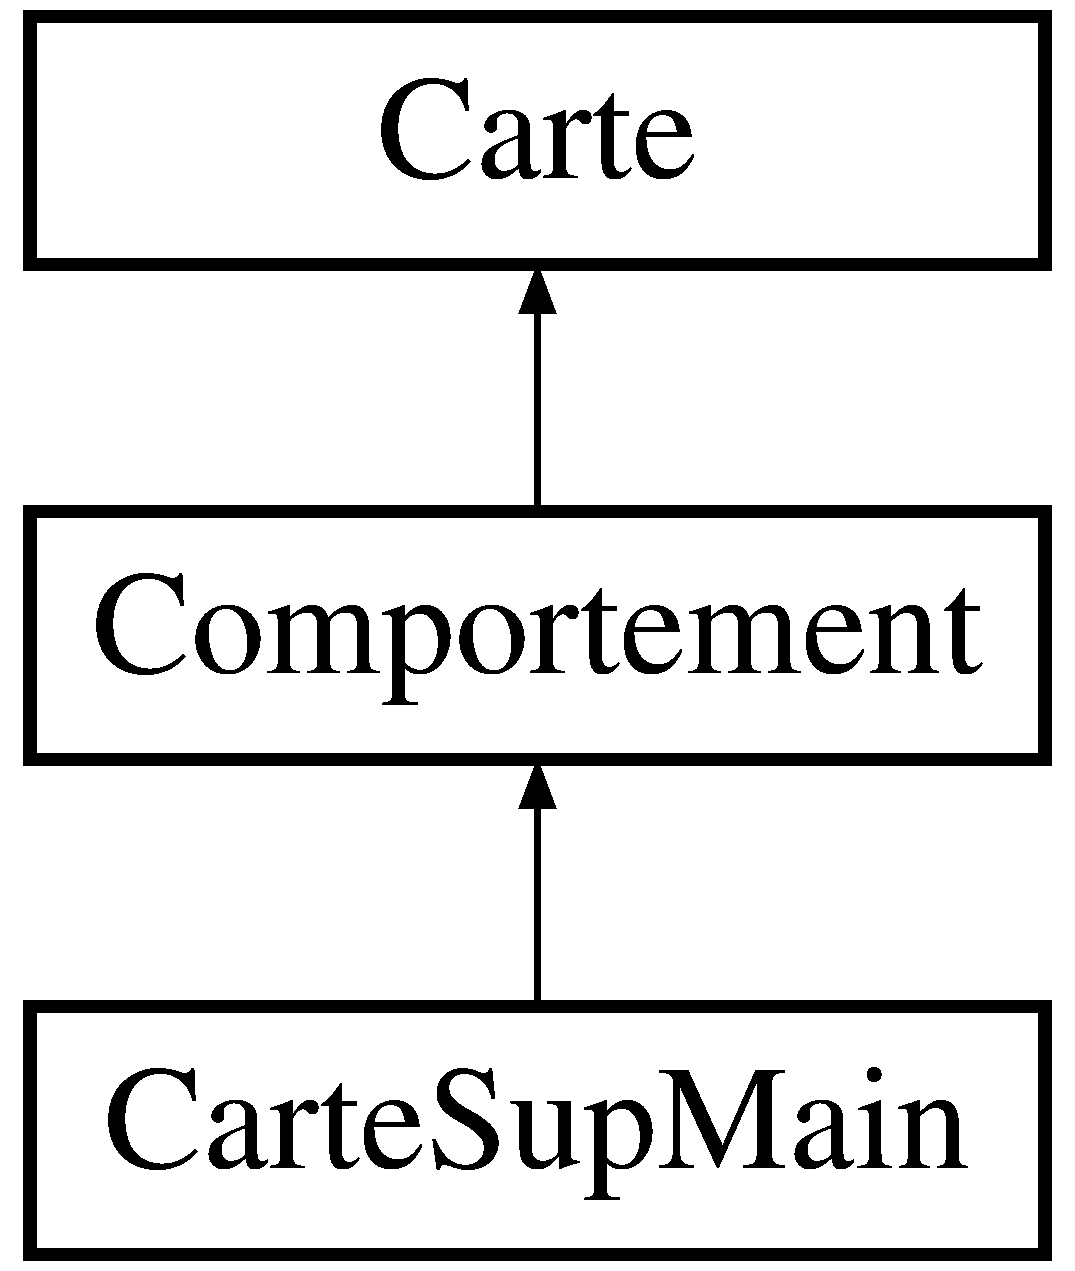
\includegraphics[height=3.000000cm]{class_carte_sup_main}
\end{center}
\end{figure}
\subsection*{Public Member Functions}
\begin{DoxyCompactItemize}
\item 
\hyperlink{class_carte_sup_main_a3b11d1f416f17dcde86201480b82b001}{Carte\-Sup\-Main} (\hyperlink{class_carte}{Carte} $\ast$c, int v)
\begin{DoxyCompactList}\small\item\em Constructeur de \hyperlink{class_carte_sup_main}{Carte\-Sup\-Main}. \end{DoxyCompactList}\item 
\hypertarget{class_carte_sup_main_a46eca6a67c7699bbea5efb219c4461f1}{\hyperlink{class_carte_sup_main_a46eca6a67c7699bbea5efb219c4461f1}{$\sim$\-Carte\-Sup\-Main} ()}\label{class_carte_sup_main_a46eca6a67c7699bbea5efb219c4461f1}

\begin{DoxyCompactList}\small\item\em Destructeur de \hyperlink{class_carte_sup_main}{Carte\-Sup\-Main}. \end{DoxyCompactList}\item 
virtual void \hyperlink{class_carte_sup_main_adc7d3cf6f6e126400abad30e874cb24e}{appliquer} (\hyperlink{class_personnage}{Personnage} $\ast$p)
\begin{DoxyCompactList}\small\item\em applique le comportement de la carte \end{DoxyCompactList}\item 
virtual void \hyperlink{class_carte_sup_main_aa2b63cb5ea72b186931bbd8f093d9e20}{retirer} (\hyperlink{class_personnage}{Personnage} $\ast$p)
\begin{DoxyCompactList}\small\item\em retire le comportement de la carte \end{DoxyCompactList}\end{DoxyCompactItemize}
\subsection*{Additional Inherited Members}


\subsection{Constructor \& Destructor Documentation}
\hypertarget{class_carte_sup_main_a3b11d1f416f17dcde86201480b82b001}{\index{Carte\-Sup\-Main@{Carte\-Sup\-Main}!Carte\-Sup\-Main@{Carte\-Sup\-Main}}
\index{Carte\-Sup\-Main@{Carte\-Sup\-Main}!CarteSupMain@{Carte\-Sup\-Main}}
\subsubsection[{Carte\-Sup\-Main}]{\setlength{\rightskip}{0pt plus 5cm}Carte\-Sup\-Main\-::\-Carte\-Sup\-Main (
\begin{DoxyParamCaption}
\item[{{\bf Carte} $\ast$}]{c, }
\item[{int}]{v}
\end{DoxyParamCaption}
)}}\label{class_carte_sup_main_a3b11d1f416f17dcde86201480b82b001}


Constructeur de \hyperlink{class_carte_sup_main}{Carte\-Sup\-Main}. 


\begin{DoxyParams}{Parameters}
{\em c} & \hyperlink{class_carte}{Carte} décorée \\
\hline
{\em valeur} & Valeur du comportement \\
\hline
\end{DoxyParams}


\subsection{Member Function Documentation}
\hypertarget{class_carte_sup_main_adc7d3cf6f6e126400abad30e874cb24e}{\index{Carte\-Sup\-Main@{Carte\-Sup\-Main}!appliquer@{appliquer}}
\index{appliquer@{appliquer}!CarteSupMain@{Carte\-Sup\-Main}}
\subsubsection[{appliquer}]{\setlength{\rightskip}{0pt plus 5cm}void Carte\-Sup\-Main\-::appliquer (
\begin{DoxyParamCaption}
\item[{{\bf Personnage} $\ast$}]{p}
\end{DoxyParamCaption}
)\hspace{0.3cm}{\ttfamily [virtual]}}}\label{class_carte_sup_main_adc7d3cf6f6e126400abad30e874cb24e}


applique le comportement de la carte 


\begin{DoxyParams}{Parameters}
{\em cible} & du comportement \\
\hline
\end{DoxyParams}


Reimplemented from \hyperlink{class_comportement_ae55149d29c710b0a5a0388cae308024f}{Comportement}.

\hypertarget{class_carte_sup_main_aa2b63cb5ea72b186931bbd8f093d9e20}{\index{Carte\-Sup\-Main@{Carte\-Sup\-Main}!retirer@{retirer}}
\index{retirer@{retirer}!CarteSupMain@{Carte\-Sup\-Main}}
\subsubsection[{retirer}]{\setlength{\rightskip}{0pt plus 5cm}void Carte\-Sup\-Main\-::retirer (
\begin{DoxyParamCaption}
\item[{{\bf Personnage} $\ast$}]{p}
\end{DoxyParamCaption}
)\hspace{0.3cm}{\ttfamily [virtual]}}}\label{class_carte_sup_main_aa2b63cb5ea72b186931bbd8f093d9e20}


retire le comportement de la carte 


\begin{DoxyParams}{Parameters}
{\em cible} & du comportement \\
\hline
\end{DoxyParams}


Reimplemented from \hyperlink{class_comportement_a7be9c46a6ae6d49ca3f49288b438b689}{Comportement}.



The documentation for this class was generated from the following files\-:\begin{DoxyCompactItemize}
\item 
\hyperlink{_carte_sup_main_8hpp}{Carte\-Sup\-Main.\-hpp}\item 
\hyperlink{_carte_sup_main_8cpp}{Carte\-Sup\-Main.\-cpp}\end{DoxyCompactItemize}

\hypertarget{class_chaussure}{\section{Chaussure Class Reference}
\label{class_chaussure}\index{Chaussure@{Chaussure}}
}
Inheritance diagram for Chaussure\-:\begin{figure}[H]
\begin{center}
\leavevmode
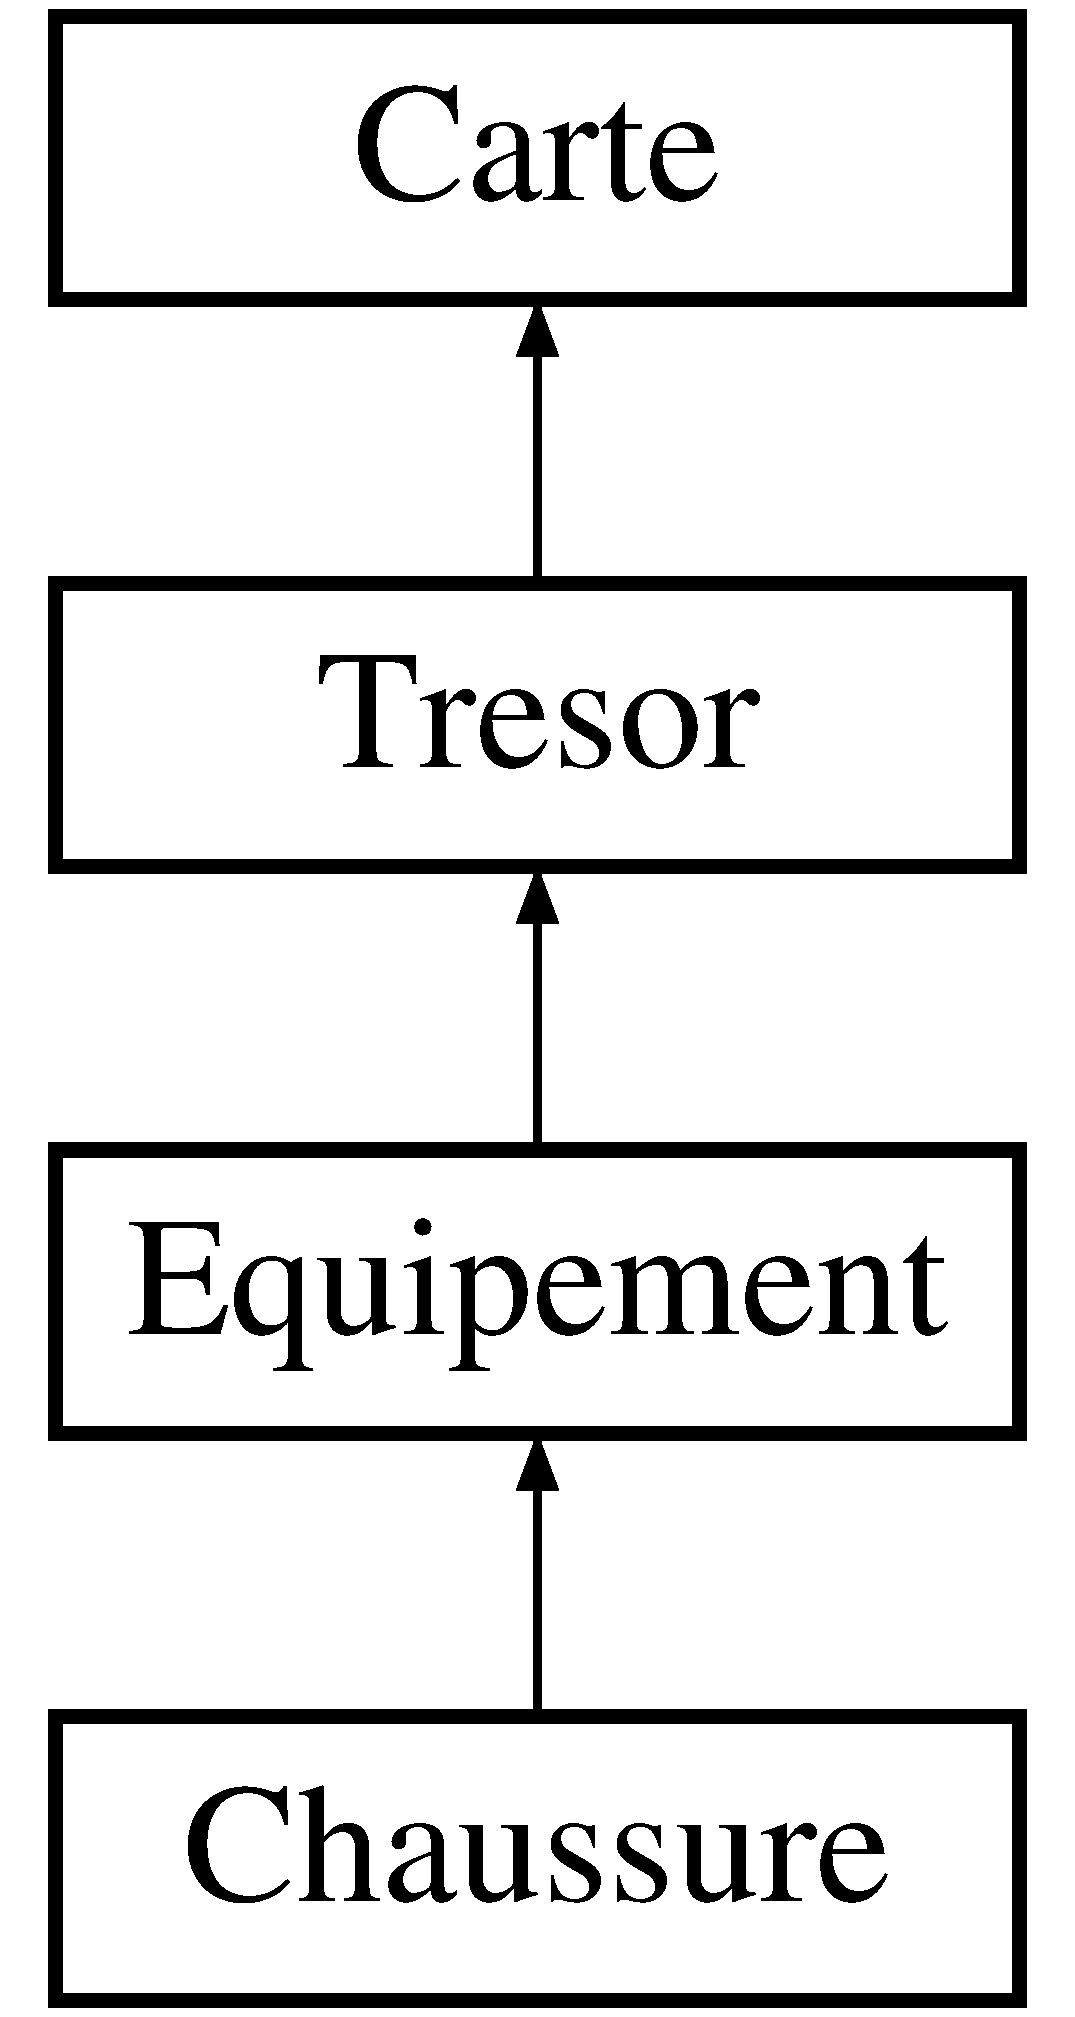
\includegraphics[height=4.000000cm]{class_chaussure}
\end{center}
\end{figure}
\subsection*{Public Member Functions}
\begin{DoxyCompactItemize}
\item 
\hyperlink{class_chaussure_a8dc525d9f3a82315d7ad82357e3f0e8f}{Chaussure} (int id, std\-::string n, std\-::string d, int p)
\begin{DoxyCompactList}\small\item\em Constructeur de \hyperlink{class_chaussure}{Chaussure}. \end{DoxyCompactList}\item 
bool \hyperlink{class_chaussure_a1d9c1abb1dc4c3bd6476fa19a5885973}{est\-Chaussure} ()
\begin{DoxyCompactList}\small\item\em Renvoie vrai si c'est une \hyperlink{class_chaussure}{Chaussure}. \end{DoxyCompactList}\end{DoxyCompactItemize}
\subsection*{Additional Inherited Members}


\subsection{Constructor \& Destructor Documentation}
\hypertarget{class_chaussure_a8dc525d9f3a82315d7ad82357e3f0e8f}{\index{Chaussure@{Chaussure}!Chaussure@{Chaussure}}
\index{Chaussure@{Chaussure}!Chaussure@{Chaussure}}
\subsubsection[{Chaussure}]{\setlength{\rightskip}{0pt plus 5cm}Chaussure\-::\-Chaussure (
\begin{DoxyParamCaption}
\item[{int}]{id, }
\item[{std\-::string}]{n, }
\item[{std\-::string}]{d, }
\item[{int}]{p}
\end{DoxyParamCaption}
)}}\label{class_chaussure_a8dc525d9f3a82315d7ad82357e3f0e8f}


Constructeur de \hyperlink{class_chaussure}{Chaussure}. 


\begin{DoxyParams}{Parameters}
{\em id} & Identifiant de la carte \\
\hline
{\em n} & nom de la carte \\
\hline
{\em d} & description de la carte \\
\hline
{\em p} & prix de la carte \\
\hline
\end{DoxyParams}


\subsection{Member Function Documentation}
\hypertarget{class_chaussure_a1d9c1abb1dc4c3bd6476fa19a5885973}{\index{Chaussure@{Chaussure}!est\-Chaussure@{est\-Chaussure}}
\index{est\-Chaussure@{est\-Chaussure}!Chaussure@{Chaussure}}
\subsubsection[{est\-Chaussure}]{\setlength{\rightskip}{0pt plus 5cm}bool Chaussure\-::est\-Chaussure (
\begin{DoxyParamCaption}
{}
\end{DoxyParamCaption}
)\hspace{0.3cm}{\ttfamily [virtual]}}}\label{class_chaussure_a1d9c1abb1dc4c3bd6476fa19a5885973}


Renvoie vrai si c'est une \hyperlink{class_chaussure}{Chaussure}. 

\begin{DoxyReturn}{Returns}
vrai si c'est une \hyperlink{class_chaussure}{Chaussure}, Faux sinon 
\end{DoxyReturn}


Reimplemented from \hyperlink{class_carte_a830cd4aac4b93fab69a0901d35e562ab}{Carte}.



The documentation for this class was generated from the following files\-:\begin{DoxyCompactItemize}
\item 
\hyperlink{_chaussure_8hpp}{Chaussure.\-hpp}\item 
Chaussure.\-cpp\end{DoxyCompactItemize}

\hypertarget{class_comportement}{\section{Comportement Class Reference}
\label{class_comportement}\index{Comportement@{Comportement}}
}
Inheritance diagram for Comportement\-:\begin{figure}[H]
\begin{center}
\leavevmode
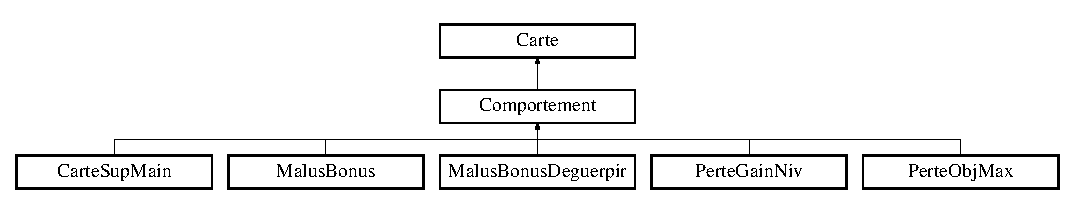
\includegraphics[height=2.301370cm]{class_comportement}
\end{center}
\end{figure}
\subsection*{Public Member Functions}
\begin{DoxyCompactItemize}
\item 
\hyperlink{class_comportement_a897f229c21410bcf3d249ce3242f07a8}{Comportement} (int id, std\-::string n, std\-::string d, \hyperlink{class_carte}{Carte} $\ast$c, int \hyperlink{class_comportement_a563bc6aa1b8ee82a698f13cac1879c7a}{valeur})
\begin{DoxyCompactList}\small\item\em Constructeur de comportement. \end{DoxyCompactList}\item 
\hypertarget{class_comportement_acbe985635ed33cf141f380720c2e3f77}{\hyperlink{class_comportement_acbe985635ed33cf141f380720c2e3f77}{$\sim$\-Comportement} ()}\label{class_comportement_acbe985635ed33cf141f380720c2e3f77}

\begin{DoxyCompactList}\small\item\em Destructeur de \hyperlink{class_comportement}{Comportement}. \end{DoxyCompactList}\item 
virtual std\-::string \hyperlink{class_comportement_a0dd697e029b781d83f3251204845530e}{get\-Nom} ()
\begin{DoxyCompactList}\small\item\em Renvoie le nom de la carte. \end{DoxyCompactList}\item 
virtual std\-::string \hyperlink{class_comportement_a534918dd72e2e3c1d2ecbd85f1c38e65}{get\-Description} ()
\begin{DoxyCompactList}\small\item\em Renvoie la description de la carte. \end{DoxyCompactList}\item 
virtual \hyperlink{class_carte}{Carte} $\ast$ \hyperlink{class_comportement_ae05651b07ef8145ae070507ea455241c}{get\-Carte} ()
\begin{DoxyCompactList}\small\item\em Renvoie un pointeur sur cet �l�ment. \end{DoxyCompactList}\item 
virtual bool \hyperlink{class_comportement_a25ae445c0424638fd2eef12123960d4b}{est\-Porte} ()
\begin{DoxyCompactList}\small\item\em Renvoie vrai si c'est une \hyperlink{class_porte}{Porte}. \end{DoxyCompactList}\item 
virtual bool \hyperlink{class_comportement_a7598241705f53e86b1d08dce11a1a4dd}{est\-Malediction} ()
\begin{DoxyCompactList}\small\item\em Renvoie vrai si c'est une \hyperlink{class_malediction}{Malediction}. \end{DoxyCompactList}\item 
virtual bool \hyperlink{class_comportement_a8cfc80bb17c61c7e5597c50609ec2cfe}{est\-Monstre} ()
\begin{DoxyCompactList}\small\item\em Renvoie vrai si c'est un \hyperlink{class_monstre}{Monstre}. \end{DoxyCompactList}\item 
virtual bool \hyperlink{class_comportement_a0aaa6b86b322e54ff2d0c1e448a650c4}{est\-Race} ()
\begin{DoxyCompactList}\small\item\em Renvoie vrai si c'est une \hyperlink{class_race}{Race}. \end{DoxyCompactList}\item 
virtual bool \hyperlink{class_comportement_a2bd892e21d3f14e5e585be037d6ec5bd}{est\-Potion} ()
\begin{DoxyCompactList}\small\item\em Renvoie vrai si c'est une \hyperlink{class_potion}{Potion}. \end{DoxyCompactList}\item 
virtual bool \hyperlink{class_comportement_aae304a510ec6096fcb4337a72f0fcd72}{est\-Equipement} ()
\begin{DoxyCompactList}\small\item\em Renvoie vrai si c'est un \hyperlink{class_equipement}{Equipement}. \end{DoxyCompactList}\item 
virtual bool \hyperlink{class_comportement_a3fc939a96fbe4154af5b104ecc7a1afd}{est\-Armure} ()
\begin{DoxyCompactList}\small\item\em Renvoie vrai si c'est une \hyperlink{class_armure}{Armure}. \end{DoxyCompactList}\item 
virtual bool \hyperlink{class_comportement_ab862b3685bf0f29f204ea96b98dc1d4b}{est\-Chaussure} ()
\begin{DoxyCompactList}\small\item\em Renvoie vrai si c'est une \hyperlink{class_chaussure}{Chaussure}. \end{DoxyCompactList}\item 
virtual bool \hyperlink{class_comportement_ae3b252fd5bd95df0d2cdfab1242db808}{est\-Couvre\-Chef} ()
\begin{DoxyCompactList}\small\item\em Renvoie vrai si c'est un \hyperlink{class_couvre_chef}{Couvre\-Chef}. \end{DoxyCompactList}\item 
virtual bool \hyperlink{class_comportement_a91ac9d0063ac95f333ab62f5034cc3ce}{est\-Main} ()
\begin{DoxyCompactList}\small\item\em Renvoie vrai si c'est une \hyperlink{class_main}{Main}. \end{DoxyCompactList}\item 
virtual void \hyperlink{class_comportement_ae55149d29c710b0a5a0388cae308024f}{appliquer} (\hyperlink{class_personnage}{Personnage} $\ast$p)
\begin{DoxyCompactList}\small\item\em applique le comportement de la carte \end{DoxyCompactList}\item 
virtual void \hyperlink{class_comportement_a7be9c46a6ae6d49ca3f49288b438b689}{retirer} (\hyperlink{class_personnage}{Personnage} $\ast$p)
\begin{DoxyCompactList}\small\item\em retire le comportement de la carte \end{DoxyCompactList}\item 
virtual int \hyperlink{class_comportement_a0aa55aa40f00b6e9a2775126e39f0de7}{get\-Valeur} ()
\begin{DoxyCompactList}\small\item\em renvoie la valeur du comportement \end{DoxyCompactList}\end{DoxyCompactItemize}
\subsection*{Protected Attributes}
\begin{DoxyCompactItemize}
\item 
\hyperlink{class_carte}{Carte} $\ast$ \hyperlink{class_comportement_a46d6db6dc879c5488c1f1aea04593f66}{carte}
\item 
int \hyperlink{class_comportement_a563bc6aa1b8ee82a698f13cac1879c7a}{valeur}
\end{DoxyCompactItemize}


\subsection{Constructor \& Destructor Documentation}
\hypertarget{class_comportement_a897f229c21410bcf3d249ce3242f07a8}{\index{Comportement@{Comportement}!Comportement@{Comportement}}
\index{Comportement@{Comportement}!Comportement@{Comportement}}
\subsubsection[{Comportement}]{\setlength{\rightskip}{0pt plus 5cm}Comportement\-::\-Comportement (
\begin{DoxyParamCaption}
\item[{int}]{id, }
\item[{std\-::string}]{n, }
\item[{std\-::string}]{d, }
\item[{{\bf Carte} $\ast$}]{c, }
\item[{int}]{valeur}
\end{DoxyParamCaption}
)}}\label{class_comportement_a897f229c21410bcf3d249ce3242f07a8}


Constructeur de comportement. 


\begin{DoxyParams}{Parameters}
{\em id} & identifiant de la carte \\
\hline
{\em n} & nom du comportement \\
\hline
{\em d} & description du comportement \\
\hline
{\em c} & \hyperlink{class_carte}{Carte} d�cor�e \\
\hline
{\em valeur} & Valeur du comportement \\
\hline
\end{DoxyParams}


\subsection{Member Function Documentation}
\hypertarget{class_comportement_ae55149d29c710b0a5a0388cae308024f}{\index{Comportement@{Comportement}!appliquer@{appliquer}}
\index{appliquer@{appliquer}!Comportement@{Comportement}}
\subsubsection[{appliquer}]{\setlength{\rightskip}{0pt plus 5cm}void Comportement\-::appliquer (
\begin{DoxyParamCaption}
\item[{{\bf Personnage} $\ast$}]{p}
\end{DoxyParamCaption}
)\hspace{0.3cm}{\ttfamily [virtual]}}}\label{class_comportement_ae55149d29c710b0a5a0388cae308024f}


applique le comportement de la carte 


\begin{DoxyParams}{Parameters}
{\em cible} & du comportement \\
\hline
\end{DoxyParams}


Reimplemented from \hyperlink{class_carte_ade8947dac978d46922ccff92aebf54f7}{Carte}.



Reimplemented in \hyperlink{class_carte_sup_main_adc7d3cf6f6e126400abad30e874cb24e}{Carte\-Sup\-Main}, \hyperlink{class_malus_bonus_aede2c45aa2a0d0f751c128e05d26fb6a}{Malus\-Bonus}, \hyperlink{class_malus_bonus_deguerpir_a703620e87d5d861ba850a3b07f61195a}{Malus\-Bonus\-Deguerpir}, \hyperlink{class_perte_gain_niv_ad72efe1c526391084768a500bb1ae4fa}{Perte\-Gain\-Niv}, and \hyperlink{class_perte_obj_max_a929e1c6370247feb937ae1835648a441}{Perte\-Obj\-Max}.

\hypertarget{class_comportement_a3fc939a96fbe4154af5b104ecc7a1afd}{\index{Comportement@{Comportement}!est\-Armure@{est\-Armure}}
\index{est\-Armure@{est\-Armure}!Comportement@{Comportement}}
\subsubsection[{est\-Armure}]{\setlength{\rightskip}{0pt plus 5cm}bool Comportement\-::est\-Armure (
\begin{DoxyParamCaption}
{}
\end{DoxyParamCaption}
)\hspace{0.3cm}{\ttfamily [virtual]}}}\label{class_comportement_a3fc939a96fbe4154af5b104ecc7a1afd}


Renvoie vrai si c'est une \hyperlink{class_armure}{Armure}. 

\begin{DoxyReturn}{Returns}
vrai si c'est une \hyperlink{class_armure}{Armure}, Faux sinon 
\end{DoxyReturn}


Reimplemented from \hyperlink{class_carte_a5d971af0574d33695afba7c525ef1a3e}{Carte}.

\hypertarget{class_comportement_ab862b3685bf0f29f204ea96b98dc1d4b}{\index{Comportement@{Comportement}!est\-Chaussure@{est\-Chaussure}}
\index{est\-Chaussure@{est\-Chaussure}!Comportement@{Comportement}}
\subsubsection[{est\-Chaussure}]{\setlength{\rightskip}{0pt plus 5cm}bool Comportement\-::est\-Chaussure (
\begin{DoxyParamCaption}
{}
\end{DoxyParamCaption}
)\hspace{0.3cm}{\ttfamily [virtual]}}}\label{class_comportement_ab862b3685bf0f29f204ea96b98dc1d4b}


Renvoie vrai si c'est une \hyperlink{class_chaussure}{Chaussure}. 

\begin{DoxyReturn}{Returns}
vrai si c'est une \hyperlink{class_chaussure}{Chaussure}, Faux sinon 
\end{DoxyReturn}


Reimplemented from \hyperlink{class_carte_a830cd4aac4b93fab69a0901d35e562ab}{Carte}.

\hypertarget{class_comportement_ae3b252fd5bd95df0d2cdfab1242db808}{\index{Comportement@{Comportement}!est\-Couvre\-Chef@{est\-Couvre\-Chef}}
\index{est\-Couvre\-Chef@{est\-Couvre\-Chef}!Comportement@{Comportement}}
\subsubsection[{est\-Couvre\-Chef}]{\setlength{\rightskip}{0pt plus 5cm}bool Comportement\-::est\-Couvre\-Chef (
\begin{DoxyParamCaption}
{}
\end{DoxyParamCaption}
)\hspace{0.3cm}{\ttfamily [virtual]}}}\label{class_comportement_ae3b252fd5bd95df0d2cdfab1242db808}


Renvoie vrai si c'est un \hyperlink{class_couvre_chef}{Couvre\-Chef}. 

\begin{DoxyReturn}{Returns}
vrai si c'est un \hyperlink{class_couvre_chef}{Couvre\-Chef}, Faux sinon 
\end{DoxyReturn}


Reimplemented from \hyperlink{class_carte_aeb1c07fe1a7071b2d6d4a14bbeb032f5}{Carte}.

\hypertarget{class_comportement_aae304a510ec6096fcb4337a72f0fcd72}{\index{Comportement@{Comportement}!est\-Equipement@{est\-Equipement}}
\index{est\-Equipement@{est\-Equipement}!Comportement@{Comportement}}
\subsubsection[{est\-Equipement}]{\setlength{\rightskip}{0pt plus 5cm}bool Comportement\-::est\-Equipement (
\begin{DoxyParamCaption}
{}
\end{DoxyParamCaption}
)\hspace{0.3cm}{\ttfamily [virtual]}}}\label{class_comportement_aae304a510ec6096fcb4337a72f0fcd72}


Renvoie vrai si c'est un \hyperlink{class_equipement}{Equipement}. 

\begin{DoxyReturn}{Returns}
vrai si c'est une \hyperlink{class_equipement}{Equipement}, Faux sinon 
\end{DoxyReturn}


Reimplemented from \hyperlink{class_carte_abcf22b28f170502cb4f17f2c0b7a031f}{Carte}.

\hypertarget{class_comportement_a91ac9d0063ac95f333ab62f5034cc3ce}{\index{Comportement@{Comportement}!est\-Main@{est\-Main}}
\index{est\-Main@{est\-Main}!Comportement@{Comportement}}
\subsubsection[{est\-Main}]{\setlength{\rightskip}{0pt plus 5cm}bool Comportement\-::est\-Main (
\begin{DoxyParamCaption}
{}
\end{DoxyParamCaption}
)\hspace{0.3cm}{\ttfamily [virtual]}}}\label{class_comportement_a91ac9d0063ac95f333ab62f5034cc3ce}


Renvoie vrai si c'est une \hyperlink{class_main}{Main}. 

\begin{DoxyReturn}{Returns}
vrai si c'est une \hyperlink{class_main}{Main}, Faux sinon 
\end{DoxyReturn}


Reimplemented from \hyperlink{class_carte_a13cfbbcd63cd11659ada554db42f6a3f}{Carte}.

\hypertarget{class_comportement_a7598241705f53e86b1d08dce11a1a4dd}{\index{Comportement@{Comportement}!est\-Malediction@{est\-Malediction}}
\index{est\-Malediction@{est\-Malediction}!Comportement@{Comportement}}
\subsubsection[{est\-Malediction}]{\setlength{\rightskip}{0pt plus 5cm}bool Comportement\-::est\-Malediction (
\begin{DoxyParamCaption}
{}
\end{DoxyParamCaption}
)\hspace{0.3cm}{\ttfamily [virtual]}}}\label{class_comportement_a7598241705f53e86b1d08dce11a1a4dd}


Renvoie vrai si c'est une \hyperlink{class_malediction}{Malediction}. 

\begin{DoxyReturn}{Returns}
vrai si c'est une \hyperlink{class_malediction}{Malediction}, Faux sinon 
\end{DoxyReturn}


Reimplemented from \hyperlink{class_carte_af9c84ec45b9a570d8ac8019726756ee7}{Carte}.

\hypertarget{class_comportement_a8cfc80bb17c61c7e5597c50609ec2cfe}{\index{Comportement@{Comportement}!est\-Monstre@{est\-Monstre}}
\index{est\-Monstre@{est\-Monstre}!Comportement@{Comportement}}
\subsubsection[{est\-Monstre}]{\setlength{\rightskip}{0pt plus 5cm}bool Comportement\-::est\-Monstre (
\begin{DoxyParamCaption}
{}
\end{DoxyParamCaption}
)\hspace{0.3cm}{\ttfamily [virtual]}}}\label{class_comportement_a8cfc80bb17c61c7e5597c50609ec2cfe}


Renvoie vrai si c'est un \hyperlink{class_monstre}{Monstre}. 

\begin{DoxyReturn}{Returns}
vrai si c'est un \hyperlink{class_monstre}{Monstre}, Faux sinon 
\end{DoxyReturn}


Reimplemented from \hyperlink{class_carte_a74c9bf2967ea099015d1b96003f9da18}{Carte}.

\hypertarget{class_comportement_a25ae445c0424638fd2eef12123960d4b}{\index{Comportement@{Comportement}!est\-Porte@{est\-Porte}}
\index{est\-Porte@{est\-Porte}!Comportement@{Comportement}}
\subsubsection[{est\-Porte}]{\setlength{\rightskip}{0pt plus 5cm}bool Comportement\-::est\-Porte (
\begin{DoxyParamCaption}
{}
\end{DoxyParamCaption}
)\hspace{0.3cm}{\ttfamily [virtual]}}}\label{class_comportement_a25ae445c0424638fd2eef12123960d4b}


Renvoie vrai si c'est une \hyperlink{class_porte}{Porte}. 

\begin{DoxyReturn}{Returns}
vrai si c'est une \hyperlink{class_porte}{Porte}, Faux sinon 
\end{DoxyReturn}


Reimplemented from \hyperlink{class_carte_af0156ad1b4b87414df65caddd310212a}{Carte}.

\hypertarget{class_comportement_a2bd892e21d3f14e5e585be037d6ec5bd}{\index{Comportement@{Comportement}!est\-Potion@{est\-Potion}}
\index{est\-Potion@{est\-Potion}!Comportement@{Comportement}}
\subsubsection[{est\-Potion}]{\setlength{\rightskip}{0pt plus 5cm}bool Comportement\-::est\-Potion (
\begin{DoxyParamCaption}
{}
\end{DoxyParamCaption}
)\hspace{0.3cm}{\ttfamily [virtual]}}}\label{class_comportement_a2bd892e21d3f14e5e585be037d6ec5bd}


Renvoie vrai si c'est une \hyperlink{class_potion}{Potion}. 

\begin{DoxyReturn}{Returns}
vrai si c'est une \hyperlink{class_potion}{Potion}, Faux sinon 
\end{DoxyReturn}


Reimplemented from \hyperlink{class_carte_a3be68ed1ee99d835cd27148e456e5b9c}{Carte}.

\hypertarget{class_comportement_a0aaa6b86b322e54ff2d0c1e448a650c4}{\index{Comportement@{Comportement}!est\-Race@{est\-Race}}
\index{est\-Race@{est\-Race}!Comportement@{Comportement}}
\subsubsection[{est\-Race}]{\setlength{\rightskip}{0pt plus 5cm}bool Comportement\-::est\-Race (
\begin{DoxyParamCaption}
{}
\end{DoxyParamCaption}
)\hspace{0.3cm}{\ttfamily [virtual]}}}\label{class_comportement_a0aaa6b86b322e54ff2d0c1e448a650c4}


Renvoie vrai si c'est une \hyperlink{class_race}{Race}. 

\begin{DoxyReturn}{Returns}
vrai si c'est une \hyperlink{class_race}{Race}, Faux sinon 
\end{DoxyReturn}


Reimplemented from \hyperlink{class_carte_acbac53716e6285801ca151aa177fc699}{Carte}.

\hypertarget{class_comportement_ae05651b07ef8145ae070507ea455241c}{\index{Comportement@{Comportement}!get\-Carte@{get\-Carte}}
\index{get\-Carte@{get\-Carte}!Comportement@{Comportement}}
\subsubsection[{get\-Carte}]{\setlength{\rightskip}{0pt plus 5cm}{\bf Carte} $\ast$ Comportement\-::get\-Carte (
\begin{DoxyParamCaption}
{}
\end{DoxyParamCaption}
)\hspace{0.3cm}{\ttfamily [virtual]}}}\label{class_comportement_ae05651b07ef8145ae070507ea455241c}


Renvoie un pointeur sur cet �l�ment. 

\begin{DoxyReturn}{Returns}
pointeur sur cet �l�ment 
\end{DoxyReturn}


Reimplemented from \hyperlink{class_carte_a03711d12e3252863aa4303b3edc5c118}{Carte}.

\hypertarget{class_comportement_a534918dd72e2e3c1d2ecbd85f1c38e65}{\index{Comportement@{Comportement}!get\-Description@{get\-Description}}
\index{get\-Description@{get\-Description}!Comportement@{Comportement}}
\subsubsection[{get\-Description}]{\setlength{\rightskip}{0pt plus 5cm}std\-::string Comportement\-::get\-Description (
\begin{DoxyParamCaption}
{}
\end{DoxyParamCaption}
)\hspace{0.3cm}{\ttfamily [virtual]}}}\label{class_comportement_a534918dd72e2e3c1d2ecbd85f1c38e65}


Renvoie la description de la carte. 

\begin{DoxyReturn}{Returns}
description de la carte 
\end{DoxyReturn}


Reimplemented from \hyperlink{class_carte_a591705d6bb95c36ce4a034b3107ae85c}{Carte}.

\hypertarget{class_comportement_a0dd697e029b781d83f3251204845530e}{\index{Comportement@{Comportement}!get\-Nom@{get\-Nom}}
\index{get\-Nom@{get\-Nom}!Comportement@{Comportement}}
\subsubsection[{get\-Nom}]{\setlength{\rightskip}{0pt plus 5cm}std\-::string Comportement\-::get\-Nom (
\begin{DoxyParamCaption}
{}
\end{DoxyParamCaption}
)\hspace{0.3cm}{\ttfamily [virtual]}}}\label{class_comportement_a0dd697e029b781d83f3251204845530e}


Renvoie le nom de la carte. 

\begin{DoxyReturn}{Returns}
nom de la carte 
\end{DoxyReturn}


Reimplemented from \hyperlink{class_carte_a7b68885ddbd8c8f6991e5447346913bc}{Carte}.

\hypertarget{class_comportement_a0aa55aa40f00b6e9a2775126e39f0de7}{\index{Comportement@{Comportement}!get\-Valeur@{get\-Valeur}}
\index{get\-Valeur@{get\-Valeur}!Comportement@{Comportement}}
\subsubsection[{get\-Valeur}]{\setlength{\rightskip}{0pt plus 5cm}int Comportement\-::get\-Valeur (
\begin{DoxyParamCaption}
{}
\end{DoxyParamCaption}
)\hspace{0.3cm}{\ttfamily [virtual]}}}\label{class_comportement_a0aa55aa40f00b6e9a2775126e39f0de7}


renvoie la valeur du comportement 

\begin{DoxyReturn}{Returns}
la valeur du comportement 
\end{DoxyReturn}


Reimplemented from \hyperlink{class_carte_ada584f087ef345e6ebf7955be74c4084}{Carte}.

\hypertarget{class_comportement_a7be9c46a6ae6d49ca3f49288b438b689}{\index{Comportement@{Comportement}!retirer@{retirer}}
\index{retirer@{retirer}!Comportement@{Comportement}}
\subsubsection[{retirer}]{\setlength{\rightskip}{0pt plus 5cm}void Comportement\-::retirer (
\begin{DoxyParamCaption}
\item[{{\bf Personnage} $\ast$}]{p}
\end{DoxyParamCaption}
)\hspace{0.3cm}{\ttfamily [virtual]}}}\label{class_comportement_a7be9c46a6ae6d49ca3f49288b438b689}


retire le comportement de la carte 


\begin{DoxyParams}{Parameters}
{\em cible} & du comportement \\
\hline
\end{DoxyParams}


Reimplemented from \hyperlink{class_carte_a938f4d4a1df46c4fc695c01e4bf585ba}{Carte}.



Reimplemented in \hyperlink{class_carte_sup_main_aa2b63cb5ea72b186931bbd8f093d9e20}{Carte\-Sup\-Main}, \hyperlink{class_malus_bonus_a213a8e9301ac84e2cf338476bf6613fc}{Malus\-Bonus}, and \hyperlink{class_malus_bonus_deguerpir_af7889dc668d138990d4e255c76bb8a89}{Malus\-Bonus\-Deguerpir}.



\subsection{Member Data Documentation}
\hypertarget{class_comportement_a46d6db6dc879c5488c1f1aea04593f66}{\index{Comportement@{Comportement}!carte@{carte}}
\index{carte@{carte}!Comportement@{Comportement}}
\subsubsection[{carte}]{\setlength{\rightskip}{0pt plus 5cm}{\bf Carte}$\ast$ Comportement\-::carte\hspace{0.3cm}{\ttfamily [protected]}}}\label{class_comportement_a46d6db6dc879c5488c1f1aea04593f66}
\hyperlink{class_carte}{Carte} d�cor�e \hypertarget{class_comportement_a563bc6aa1b8ee82a698f13cac1879c7a}{\index{Comportement@{Comportement}!valeur@{valeur}}
\index{valeur@{valeur}!Comportement@{Comportement}}
\subsubsection[{valeur}]{\setlength{\rightskip}{0pt plus 5cm}int Comportement\-::valeur\hspace{0.3cm}{\ttfamily [protected]}}}\label{class_comportement_a563bc6aa1b8ee82a698f13cac1879c7a}
valeur du comportement 

The documentation for this class was generated from the following files\-:\begin{DoxyCompactItemize}
\item 
\hyperlink{_comportement_8hpp}{Comportement.\-hpp}\item 
\hyperlink{_comportement_8cpp}{Comportement.\-cpp}\end{DoxyCompactItemize}

\hypertarget{class_couvre_chef}{\section{Couvre\-Chef Class Reference}
\label{class_couvre_chef}\index{Couvre\-Chef@{Couvre\-Chef}}
}
Inheritance diagram for Couvre\-Chef\-:\begin{figure}[H]
\begin{center}
\leavevmode
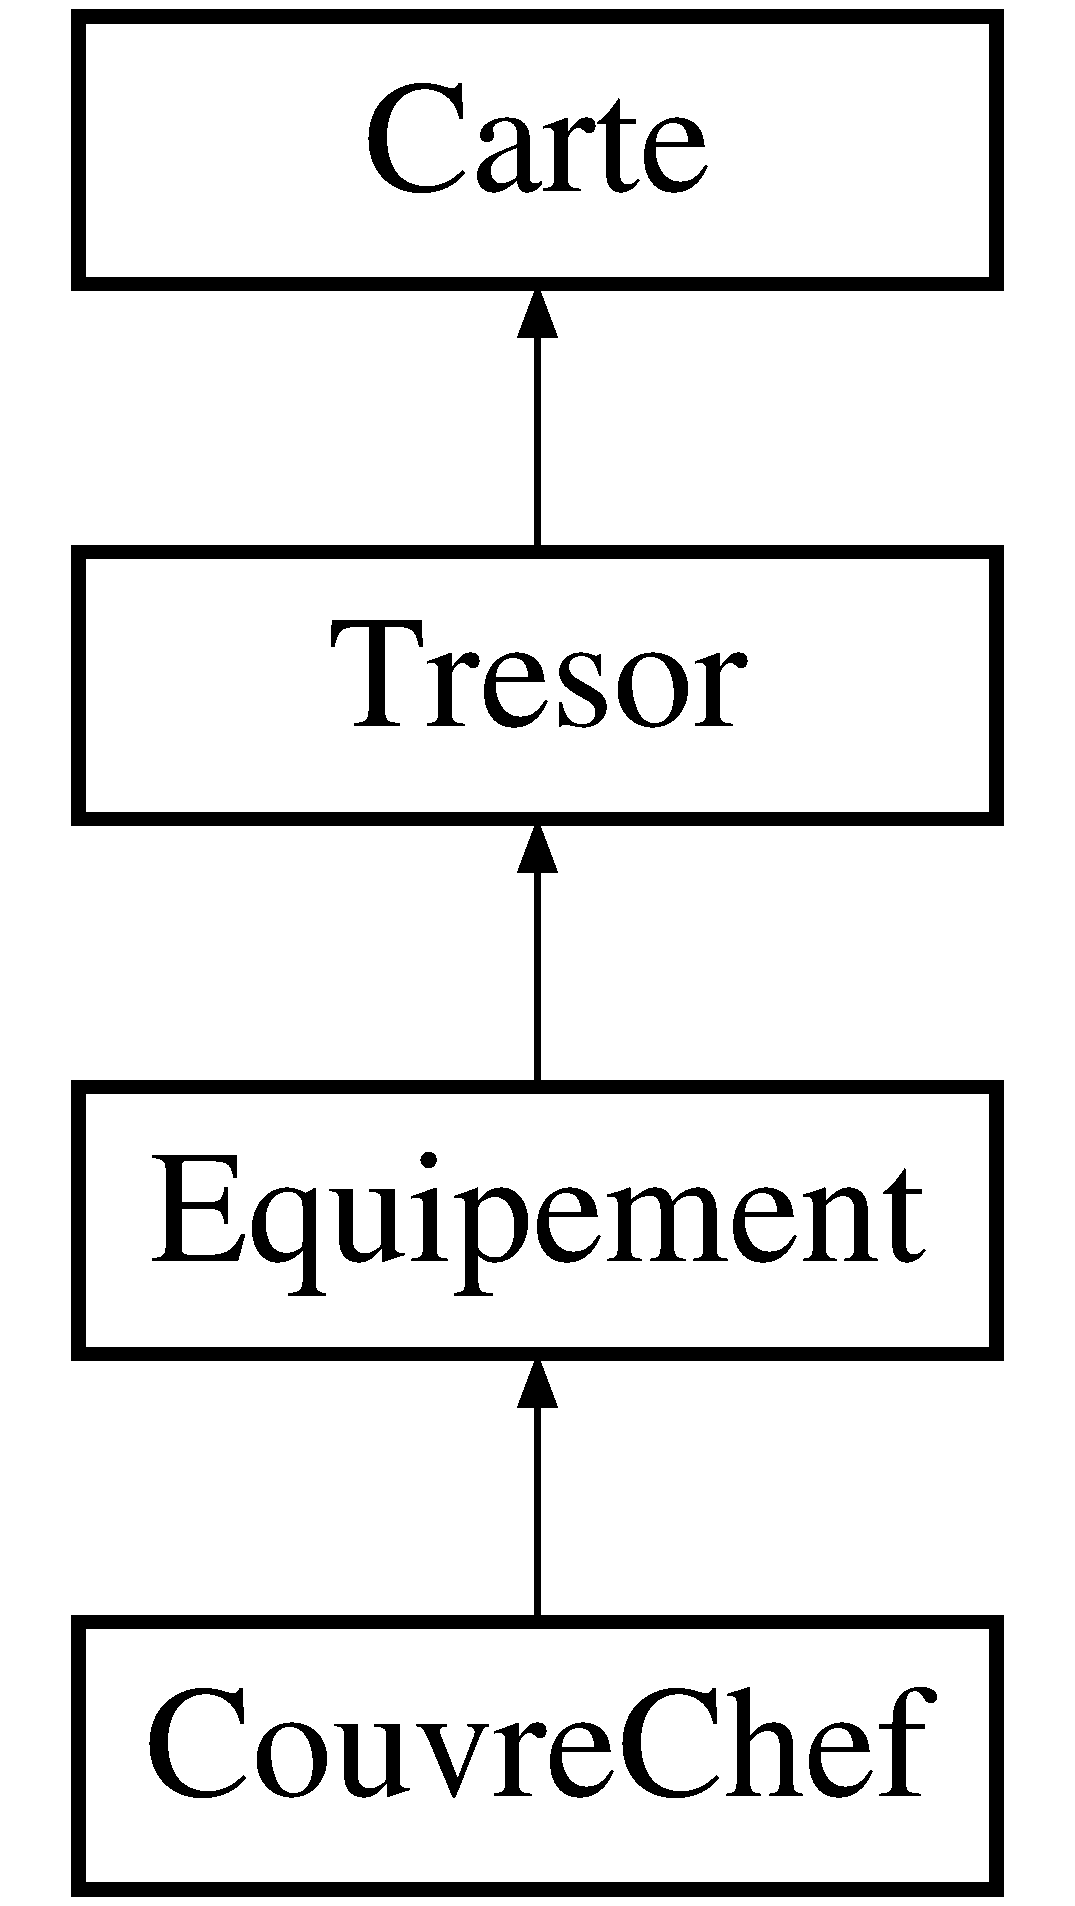
\includegraphics[height=4.000000cm]{class_couvre_chef}
\end{center}
\end{figure}
\subsection*{Public Member Functions}
\begin{DoxyCompactItemize}
\item 
\hyperlink{class_couvre_chef_a23be37af57041143163fde3d845f8239}{Couvre\-Chef} (int id, std\-::string n, std\-::string d, int p)
\begin{DoxyCompactList}\small\item\em Constructeur de \hyperlink{class_couvre_chef}{Couvre\-Chef}. \end{DoxyCompactList}\item 
bool \hyperlink{class_couvre_chef_a1fab97ed5b18d67c5dd40f5fa49c1a02}{est\-Couvre\-Chef} ()
\begin{DoxyCompactList}\small\item\em Renvoie vrai si c'est un \hyperlink{class_couvre_chef}{Couvre\-Chef}. \end{DoxyCompactList}\end{DoxyCompactItemize}
\subsection*{Additional Inherited Members}


\subsection{Constructor \& Destructor Documentation}
\hypertarget{class_couvre_chef_a23be37af57041143163fde3d845f8239}{\index{Couvre\-Chef@{Couvre\-Chef}!Couvre\-Chef@{Couvre\-Chef}}
\index{Couvre\-Chef@{Couvre\-Chef}!CouvreChef@{Couvre\-Chef}}
\subsubsection[{Couvre\-Chef}]{\setlength{\rightskip}{0pt plus 5cm}Couvre\-Chef\-::\-Couvre\-Chef (
\begin{DoxyParamCaption}
\item[{int}]{id, }
\item[{std\-::string}]{n, }
\item[{std\-::string}]{d, }
\item[{int}]{p}
\end{DoxyParamCaption}
)}}\label{class_couvre_chef_a23be37af57041143163fde3d845f8239}


Constructeur de \hyperlink{class_couvre_chef}{Couvre\-Chef}. 


\begin{DoxyParams}{Parameters}
{\em id} & Identifiant de la carte \\
\hline
{\em n} & nom de la carte \\
\hline
{\em d} & description de la carte \\
\hline
{\em p} & prix de la carte \\
\hline
\end{DoxyParams}


\subsection{Member Function Documentation}
\hypertarget{class_couvre_chef_a1fab97ed5b18d67c5dd40f5fa49c1a02}{\index{Couvre\-Chef@{Couvre\-Chef}!est\-Couvre\-Chef@{est\-Couvre\-Chef}}
\index{est\-Couvre\-Chef@{est\-Couvre\-Chef}!CouvreChef@{Couvre\-Chef}}
\subsubsection[{est\-Couvre\-Chef}]{\setlength{\rightskip}{0pt plus 5cm}bool Couvre\-Chef\-::est\-Couvre\-Chef (
\begin{DoxyParamCaption}
{}
\end{DoxyParamCaption}
)\hspace{0.3cm}{\ttfamily [virtual]}}}\label{class_couvre_chef_a1fab97ed5b18d67c5dd40f5fa49c1a02}


Renvoie vrai si c'est un \hyperlink{class_couvre_chef}{Couvre\-Chef}. 

\begin{DoxyReturn}{Returns}
vrai si c'est un \hyperlink{class_couvre_chef}{Couvre\-Chef}, Faux sinon 
\end{DoxyReturn}


Reimplemented from \hyperlink{class_carte_aeb1c07fe1a7071b2d6d4a14bbeb032f5}{Carte}.



The documentation for this class was generated from the following files\-:\begin{DoxyCompactItemize}
\item 
\hyperlink{_couvre_chef_8hpp}{Couvre\-Chef.\-hpp}\item 
Couvre\-Chef.\-cpp\end{DoxyCompactItemize}

\hypertarget{class_debut_tour}{\section{Debut\-Tour Class Reference}
\label{class_debut_tour}\index{Debut\-Tour@{Debut\-Tour}}
}
Inheritance diagram for Debut\-Tour\-:\begin{figure}[H]
\begin{center}
\leavevmode
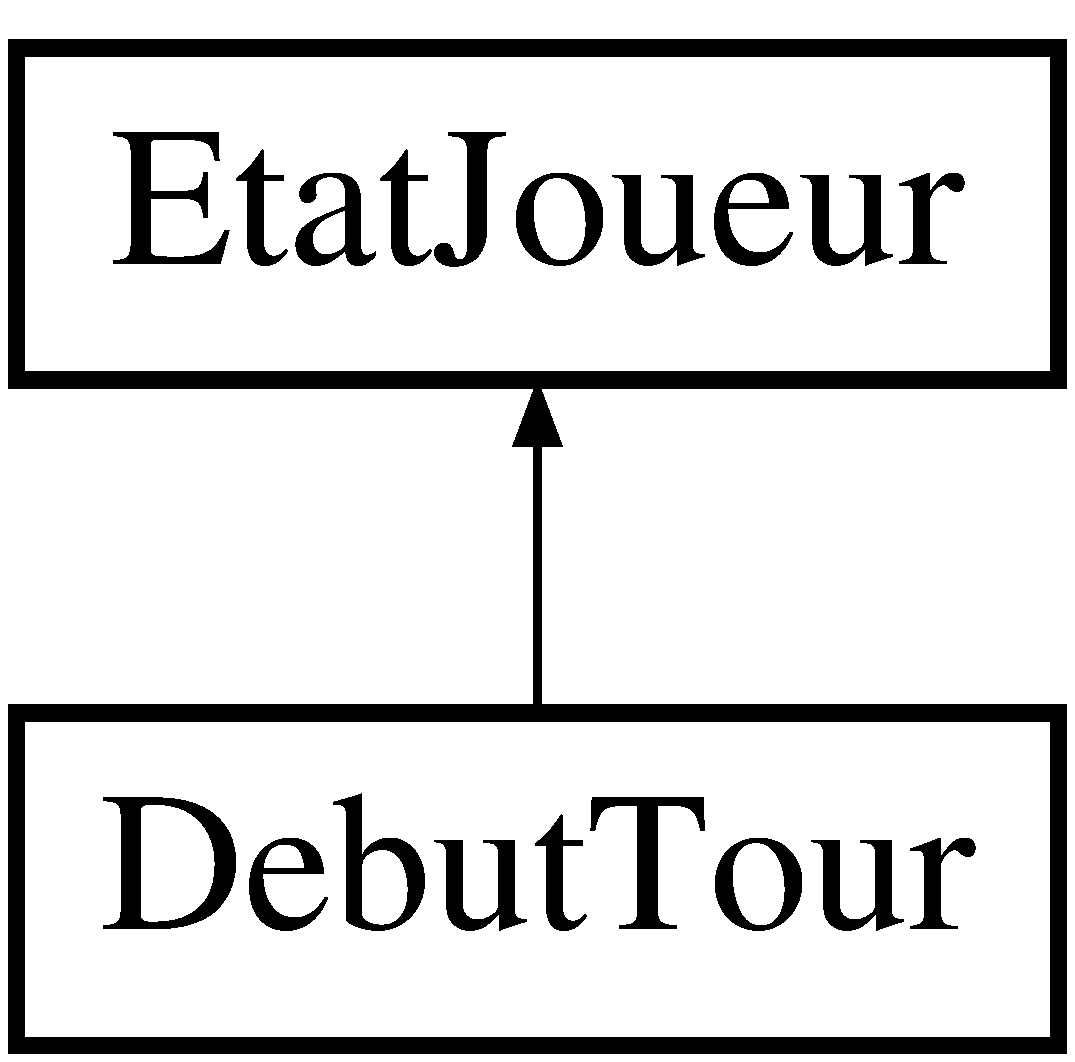
\includegraphics[height=2.000000cm]{class_debut_tour}
\end{center}
\end{figure}
\subsection*{Public Member Functions}
\begin{DoxyCompactItemize}
\item 
\hyperlink{class_debut_tour_a3acccdb6ccd60c733d00e2817bda5b17}{Debut\-Tour} (\hyperlink{class_joueur}{Joueur} $\ast$t)
\begin{DoxyCompactList}\small\item\em Constructeur de \hyperlink{class_debut_tour}{Debut\-Tour}. \end{DoxyCompactList}\item 
\hypertarget{class_debut_tour_a95f1449c91af3e1e68d213f087e14cb2}{virtual \hyperlink{class_debut_tour_a95f1449c91af3e1e68d213f087e14cb2}{$\sim$\-Debut\-Tour} ()}\label{class_debut_tour_a95f1449c91af3e1e68d213f087e14cb2}

\begin{DoxyCompactList}\small\item\em Destructeur de \hyperlink{class_debut_tour}{Debut\-Tour}. \end{DoxyCompactList}\item 
\hypertarget{class_debut_tour_a6dc0284fd0e955798e3af4220014c2d5}{void \hyperlink{class_debut_tour_a6dc0284fd0e955798e3af4220014c2d5}{piocher\-Porte\-Face\-Visible} ()}\label{class_debut_tour_a6dc0284fd0e955798e3af4220014c2d5}

\begin{DoxyCompactList}\small\item\em Permet au joueur de piocher une carte porte face visible. \end{DoxyCompactList}\item 
void \hyperlink{class_debut_tour_ae637c2d856e4f96caeb6c3f5832a4de3}{changer\-Race} (\hyperlink{class_carte}{Carte} $\ast$r)
\begin{DoxyCompactList}\small\item\em Permet au joueur de changer de race. \end{DoxyCompactList}\item 
void \hyperlink{class_debut_tour_ab2984a9914bf4ad557918a03c7430eff}{pose\-Equipement} (\hyperlink{class_carte}{Carte} $\ast$e)
\begin{DoxyCompactList}\small\item\em Permet au joueur de poser un équipement. \end{DoxyCompactList}\item 
void \hyperlink{class_debut_tour_a6c0c2462288338c678743d02b4b42883}{equiper} (\hyperlink{class_carte}{Carte} $\ast$e)
\begin{DoxyCompactList}\small\item\em Permet au joueur d'équiper un équipement. \end{DoxyCompactList}\item 
void \hyperlink{class_debut_tour_aeb01b4744259f8da83b42ca79863080c}{poser\-Malediction} (\hyperlink{class_joueur}{Joueur} $\ast$cible, \hyperlink{class_carte}{Carte} $\ast$m)
\begin{DoxyCompactList}\small\item\em Permet au joueur de poser une malédiction contre un autre joueur. \end{DoxyCompactList}\end{DoxyCompactItemize}
\subsection*{Additional Inherited Members}


\subsection{Constructor \& Destructor Documentation}
\hypertarget{class_debut_tour_a3acccdb6ccd60c733d00e2817bda5b17}{\index{Debut\-Tour@{Debut\-Tour}!Debut\-Tour@{Debut\-Tour}}
\index{Debut\-Tour@{Debut\-Tour}!DebutTour@{Debut\-Tour}}
\subsubsection[{Debut\-Tour}]{\setlength{\rightskip}{0pt plus 5cm}Debut\-Tour\-::\-Debut\-Tour (
\begin{DoxyParamCaption}
\item[{{\bf Joueur} $\ast$}]{t}
\end{DoxyParamCaption}
)}}\label{class_debut_tour_a3acccdb6ccd60c733d00e2817bda5b17}


Constructeur de \hyperlink{class_debut_tour}{Debut\-Tour}. 


\begin{DoxyParams}{Parameters}
{\em t} & \hyperlink{class_joueur}{Joueur} dont l'état doit être géré \\
\hline
\end{DoxyParams}


\subsection{Member Function Documentation}
\hypertarget{class_debut_tour_ae637c2d856e4f96caeb6c3f5832a4de3}{\index{Debut\-Tour@{Debut\-Tour}!changer\-Race@{changer\-Race}}
\index{changer\-Race@{changer\-Race}!DebutTour@{Debut\-Tour}}
\subsubsection[{changer\-Race}]{\setlength{\rightskip}{0pt plus 5cm}void Debut\-Tour\-::changer\-Race (
\begin{DoxyParamCaption}
\item[{{\bf Carte} $\ast$}]{r}
\end{DoxyParamCaption}
)\hspace{0.3cm}{\ttfamily [virtual]}}}\label{class_debut_tour_ae637c2d856e4f96caeb6c3f5832a4de3}


Permet au joueur de changer de race. 


\begin{DoxyParams}{Parameters}
{\em r} & nouvelle race \\
\hline
\end{DoxyParams}


Reimplemented from \hyperlink{class_etat_joueur_ad60942aa96f0bfb05771f787964887fe}{Etat\-Joueur}.

\hypertarget{class_debut_tour_a6c0c2462288338c678743d02b4b42883}{\index{Debut\-Tour@{Debut\-Tour}!equiper@{equiper}}
\index{equiper@{equiper}!DebutTour@{Debut\-Tour}}
\subsubsection[{equiper}]{\setlength{\rightskip}{0pt plus 5cm}void Debut\-Tour\-::equiper (
\begin{DoxyParamCaption}
\item[{{\bf Carte} $\ast$}]{e}
\end{DoxyParamCaption}
)\hspace{0.3cm}{\ttfamily [virtual]}}}\label{class_debut_tour_a6c0c2462288338c678743d02b4b42883}


Permet au joueur d'équiper un équipement. 


\begin{DoxyParams}{Parameters}
{\em e} & equipement à équiper \\
\hline
\end{DoxyParams}


Reimplemented from \hyperlink{class_etat_joueur_a2d975d2cd1163a43d6f0002c1f9943e9}{Etat\-Joueur}.

\hypertarget{class_debut_tour_ab2984a9914bf4ad557918a03c7430eff}{\index{Debut\-Tour@{Debut\-Tour}!pose\-Equipement@{pose\-Equipement}}
\index{pose\-Equipement@{pose\-Equipement}!DebutTour@{Debut\-Tour}}
\subsubsection[{pose\-Equipement}]{\setlength{\rightskip}{0pt plus 5cm}void Debut\-Tour\-::pose\-Equipement (
\begin{DoxyParamCaption}
\item[{{\bf Carte} $\ast$}]{e}
\end{DoxyParamCaption}
)\hspace{0.3cm}{\ttfamily [virtual]}}}\label{class_debut_tour_ab2984a9914bf4ad557918a03c7430eff}


Permet au joueur de poser un équipement. 


\begin{DoxyParams}{Parameters}
{\em e} & equipement à poser \\
\hline
\end{DoxyParams}


Reimplemented from \hyperlink{class_etat_joueur_a7d3b72dd7a93a787dcea00d606e9eec2}{Etat\-Joueur}.

\hypertarget{class_debut_tour_aeb01b4744259f8da83b42ca79863080c}{\index{Debut\-Tour@{Debut\-Tour}!poser\-Malediction@{poser\-Malediction}}
\index{poser\-Malediction@{poser\-Malediction}!DebutTour@{Debut\-Tour}}
\subsubsection[{poser\-Malediction}]{\setlength{\rightskip}{0pt plus 5cm}void Debut\-Tour\-::poser\-Malediction (
\begin{DoxyParamCaption}
\item[{{\bf Joueur} $\ast$}]{cible, }
\item[{{\bf Carte} $\ast$}]{m}
\end{DoxyParamCaption}
)\hspace{0.3cm}{\ttfamily [virtual]}}}\label{class_debut_tour_aeb01b4744259f8da83b42ca79863080c}


Permet au joueur de poser une malédiction contre un autre joueur. 


\begin{DoxyParams}{Parameters}
{\em cible} & cible de la malédiction \\
\hline
{\em m} & \hyperlink{class_malediction}{Malediction} à poser \\
\hline
\end{DoxyParams}


Reimplemented from \hyperlink{class_etat_joueur_a6895655263daefa056c3ee11f716cc28}{Etat\-Joueur}.



The documentation for this class was generated from the following files\-:\begin{DoxyCompactItemize}
\item 
\hyperlink{_debut_tour_8hpp}{Debut\-Tour.\-hpp}\item 
\hyperlink{_debut_tour_8cpp}{Debut\-Tour.\-cpp}\end{DoxyCompactItemize}

\hypertarget{class_equipement}{\section{Equipement Class Reference}
\label{class_equipement}\index{Equipement@{Equipement}}
}
Inheritance diagram for Equipement\-:\begin{figure}[H]
\begin{center}
\leavevmode
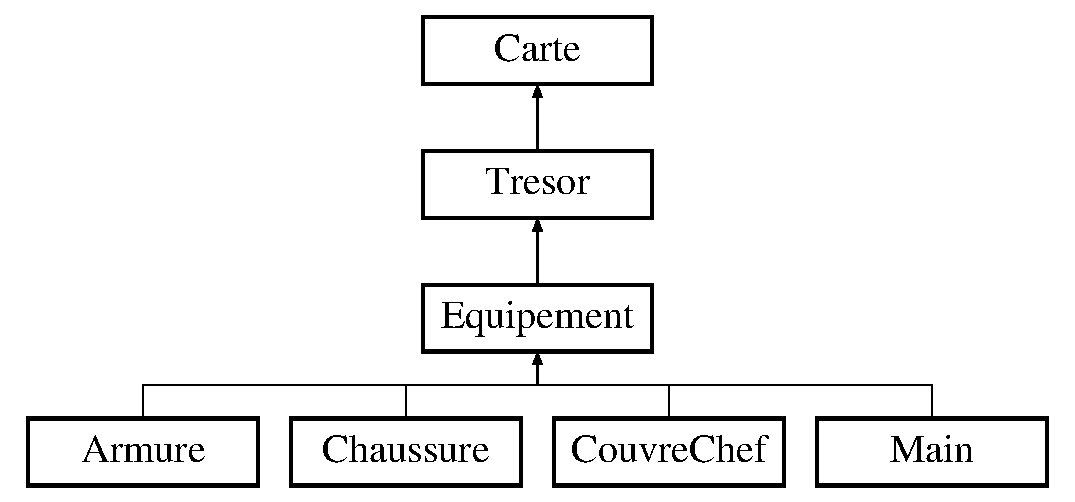
\includegraphics[height=4.000000cm]{class_equipement}
\end{center}
\end{figure}
\subsection*{Public Member Functions}
\begin{DoxyCompactItemize}
\item 
\hyperlink{class_equipement_a9d04060545423a9da1b0f6ec1b7b79b1}{Equipement} (int id, std\-::string n, std\-::string d, int p)
\begin{DoxyCompactList}\small\item\em Constructeur de \hyperlink{class_equipement}{Equipement}. \end{DoxyCompactList}\item 
\hypertarget{class_equipement_ae7751a52f2665d9e4b3e2cd6929bd986}{\hyperlink{class_equipement_ae7751a52f2665d9e4b3e2cd6929bd986}{$\sim$\-Equipement} ()}\label{class_equipement_ae7751a52f2665d9e4b3e2cd6929bd986}

\begin{DoxyCompactList}\small\item\em Destructeur de \hyperlink{class_equipement}{Equipement}. \end{DoxyCompactList}\item 
bool \hyperlink{class_equipement_ab720166d5e8dd681224de3d9490c106d}{est\-Equipement} ()
\begin{DoxyCompactList}\small\item\em Renvoie vrai si c'est un \hyperlink{class_equipement}{Equipement}. \end{DoxyCompactList}\end{DoxyCompactItemize}
\subsection*{Additional Inherited Members}


\subsection{Constructor \& Destructor Documentation}
\hypertarget{class_equipement_a9d04060545423a9da1b0f6ec1b7b79b1}{\index{Equipement@{Equipement}!Equipement@{Equipement}}
\index{Equipement@{Equipement}!Equipement@{Equipement}}
\subsubsection[{Equipement}]{\setlength{\rightskip}{0pt plus 5cm}Equipement\-::\-Equipement (
\begin{DoxyParamCaption}
\item[{int}]{id, }
\item[{std\-::string}]{n, }
\item[{std\-::string}]{d, }
\item[{int}]{p}
\end{DoxyParamCaption}
)}}\label{class_equipement_a9d04060545423a9da1b0f6ec1b7b79b1}


Constructeur de \hyperlink{class_equipement}{Equipement}. 


\begin{DoxyParams}{Parameters}
{\em id} & Identifiant de la carte \\
\hline
{\em n} & nom de la carte \\
\hline
{\em d} & description de la carte \\
\hline
{\em p} & prix de la carte \\
\hline
\end{DoxyParams}


\subsection{Member Function Documentation}
\hypertarget{class_equipement_ab720166d5e8dd681224de3d9490c106d}{\index{Equipement@{Equipement}!est\-Equipement@{est\-Equipement}}
\index{est\-Equipement@{est\-Equipement}!Equipement@{Equipement}}
\subsubsection[{est\-Equipement}]{\setlength{\rightskip}{0pt plus 5cm}bool Equipement\-::est\-Equipement (
\begin{DoxyParamCaption}
{}
\end{DoxyParamCaption}
)\hspace{0.3cm}{\ttfamily [virtual]}}}\label{class_equipement_ab720166d5e8dd681224de3d9490c106d}


Renvoie vrai si c'est un \hyperlink{class_equipement}{Equipement}. 

\begin{DoxyReturn}{Returns}
vrai si c'est une \hyperlink{class_equipement}{Equipement}, Faux sinon 
\end{DoxyReturn}


Reimplemented from \hyperlink{class_carte_abcf22b28f170502cb4f17f2c0b7a031f}{Carte}.



The documentation for this class was generated from the following files\-:\begin{DoxyCompactItemize}
\item 
\hyperlink{_equipement_8hpp}{Equipement.\-hpp}\item 
\hyperlink{_equipement_8cpp}{Equipement.\-cpp}\end{DoxyCompactItemize}

\hypertarget{class_etat_joueur}{\section{Etat\-Joueur Class Reference}
\label{class_etat_joueur}\index{Etat\-Joueur@{Etat\-Joueur}}
}
Inheritance diagram for Etat\-Joueur\-:\begin{figure}[H]
\begin{center}
\leavevmode
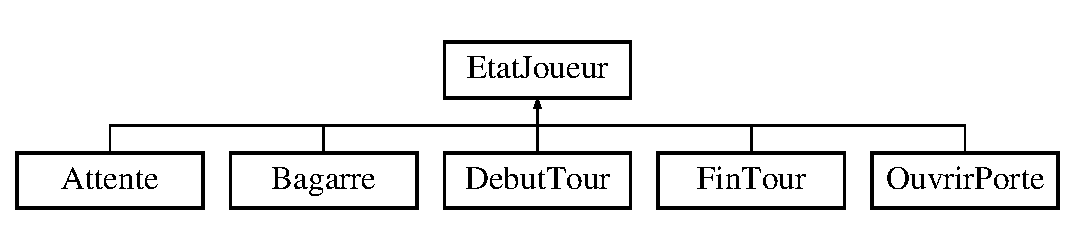
\includegraphics[height=2.000000cm]{class_etat_joueur}
\end{center}
\end{figure}
\subsection*{Public Member Functions}
\begin{DoxyCompactItemize}
\item 
\hyperlink{class_etat_joueur_a1f46122ff2c76ef26731f459ce2d4f45}{Etat\-Joueur} (\hyperlink{class_joueur}{Joueur} $\ast$t)
\begin{DoxyCompactList}\small\item\em Constructeur de \hyperlink{class_etat_joueur}{Etat\-Joueur}. \end{DoxyCompactList}\item 
\hypertarget{class_etat_joueur_acf48f30ed257324bcbac1376df584ea1}{virtual \hyperlink{class_etat_joueur_acf48f30ed257324bcbac1376df584ea1}{$\sim$\-Etat\-Joueur} ()}\label{class_etat_joueur_acf48f30ed257324bcbac1376df584ea1}

\begin{DoxyCompactList}\small\item\em Destructeur de \hyperlink{class_etat_joueur}{Etat\-Joueur}. \end{DoxyCompactList}\item 
virtual void \hyperlink{class_etat_joueur_a43fd1564d3c52d723b42ce58aaf9fb8d}{piocher\-Porte\-Face\-Visible} ()
\begin{DoxyCompactList}\small\item\em Permet au joueur de piocher une carte porte face visible. \end{DoxyCompactList}\item 
\hypertarget{class_etat_joueur_a6e1cd736b5a9ffe254948329bddabf53}{virtual void {\bfseries piocher\-Porte\-Face\-Cache} ()}\label{class_etat_joueur_a6e1cd736b5a9ffe254948329bddabf53}

\item 
virtual void \hyperlink{class_etat_joueur_ad60942aa96f0bfb05771f787964887fe}{changer\-Race} (\hyperlink{class_carte}{Carte} $\ast$r)
\begin{DoxyCompactList}\small\item\em Permet au joueur de changer de race. \end{DoxyCompactList}\item 
virtual void \hyperlink{class_etat_joueur_a7d3b72dd7a93a787dcea00d606e9eec2}{pose\-Equipement} (\hyperlink{class_carte}{Carte} $\ast$e)
\begin{DoxyCompactList}\small\item\em Permet au joueur de poser un équipement. \end{DoxyCompactList}\item 
virtual void \hyperlink{class_etat_joueur_a2d975d2cd1163a43d6f0002c1f9943e9}{equiper} (\hyperlink{class_carte}{Carte} $\ast$e)
\begin{DoxyCompactList}\small\item\em Permet au joueur d'équiper un équipement. \end{DoxyCompactList}\item 
virtual void \hyperlink{class_etat_joueur_a63c672f1d599a82f88aa80aebedf78d6}{combattre} (\hyperlink{class_carte}{Carte} $\ast$m)
\begin{DoxyCompactList}\small\item\em Permet au joueur de combattre un monstre. \end{DoxyCompactList}\item 
virtual void \hyperlink{class_etat_joueur_a6895655263daefa056c3ee11f716cc28}{poser\-Malediction} (\hyperlink{class_joueur}{Joueur} $\ast$cible, \hyperlink{class_carte}{Carte} $\ast$m)
\begin{DoxyCompactList}\small\item\em Permet au joueur de poser une malédiction contre un autre joueur. \end{DoxyCompactList}\item 
virtual void \hyperlink{class_etat_joueur_a76cf1ff3d4140f182a07167a5053f509}{poser\-Potion} (\hyperlink{class_personnage}{Personnage} $\ast$p, \hyperlink{class_carte}{Carte} $\ast$po)
\begin{DoxyCompactList}\small\item\em Permet au joueur de poser une potion. \end{DoxyCompactList}\item 
\hypertarget{class_etat_joueur_ab2184107646810a3a54f95e1b29acc57}{virtual void \hyperlink{class_etat_joueur_ab2184107646810a3a54f95e1b29acc57}{deguerpir} ()}\label{class_etat_joueur_ab2184107646810a3a54f95e1b29acc57}

\begin{DoxyCompactList}\small\item\em Permet au joueur de deguerpir lorsqu'il est en combat. \end{DoxyCompactList}\item 
virtual void \hyperlink{class_etat_joueur_a64113ef4494fa9acb088e3d125378735}{defausser\-Carte} (\hyperlink{class_carte}{Carte} $\ast$c)
\begin{DoxyCompactList}\small\item\em Permet au joueur de défausser des cartes. \end{DoxyCompactList}\item 
\hypertarget{class_etat_joueur_aaf448c35b13bc492f645c47c176d9365}{virtual void \hyperlink{class_etat_joueur_aaf448c35b13bc492f645c47c176d9365}{finir\-Tour} ()}\label{class_etat_joueur_aaf448c35b13bc492f645c47c176d9365}

\begin{DoxyCompactList}\small\item\em Permet au joueur de finir son tour. \end{DoxyCompactList}\end{DoxyCompactItemize}
\subsection*{Protected Attributes}
\begin{DoxyCompactItemize}
\item 
\hyperlink{class_joueur}{Joueur} $\ast$ \hyperlink{class_etat_joueur_a268f5c0a90e0501233fad4407508e41b}{joueur}
\end{DoxyCompactItemize}


\subsection{Constructor \& Destructor Documentation}
\hypertarget{class_etat_joueur_a1f46122ff2c76ef26731f459ce2d4f45}{\index{Etat\-Joueur@{Etat\-Joueur}!Etat\-Joueur@{Etat\-Joueur}}
\index{Etat\-Joueur@{Etat\-Joueur}!EtatJoueur@{Etat\-Joueur}}
\subsubsection[{Etat\-Joueur}]{\setlength{\rightskip}{0pt plus 5cm}Etat\-Joueur\-::\-Etat\-Joueur (
\begin{DoxyParamCaption}
\item[{{\bf Joueur} $\ast$}]{t}
\end{DoxyParamCaption}
)}}\label{class_etat_joueur_a1f46122ff2c76ef26731f459ce2d4f45}


Constructeur de \hyperlink{class_etat_joueur}{Etat\-Joueur}. 


\begin{DoxyParams}{Parameters}
{\em t} & \hyperlink{class_joueur}{Joueur} dont l'état doit être géré \\
\hline
\end{DoxyParams}


\subsection{Member Function Documentation}
\hypertarget{class_etat_joueur_ad60942aa96f0bfb05771f787964887fe}{\index{Etat\-Joueur@{Etat\-Joueur}!changer\-Race@{changer\-Race}}
\index{changer\-Race@{changer\-Race}!EtatJoueur@{Etat\-Joueur}}
\subsubsection[{changer\-Race}]{\setlength{\rightskip}{0pt plus 5cm}void Etat\-Joueur\-::changer\-Race (
\begin{DoxyParamCaption}
\item[{{\bf Carte} $\ast$}]{r}
\end{DoxyParamCaption}
)\hspace{0.3cm}{\ttfamily [virtual]}}}\label{class_etat_joueur_ad60942aa96f0bfb05771f787964887fe}


Permet au joueur de changer de race. 


\begin{DoxyParams}{Parameters}
{\em r} & nouvelle race \\
\hline
\end{DoxyParams}


Reimplemented in \hyperlink{class_fin_tour_a6b217f7a319c9daba98722b86b30da66}{Fin\-Tour}, \hyperlink{class_ouvrir_porte_acd6f890c0ed89e08cb820f547c111591}{Ouvrir\-Porte}, and \hyperlink{class_debut_tour_ae637c2d856e4f96caeb6c3f5832a4de3}{Debut\-Tour}.

\hypertarget{class_etat_joueur_a63c672f1d599a82f88aa80aebedf78d6}{\index{Etat\-Joueur@{Etat\-Joueur}!combattre@{combattre}}
\index{combattre@{combattre}!EtatJoueur@{Etat\-Joueur}}
\subsubsection[{combattre}]{\setlength{\rightskip}{0pt plus 5cm}void Etat\-Joueur\-::combattre (
\begin{DoxyParamCaption}
\item[{{\bf Carte} $\ast$}]{m}
\end{DoxyParamCaption}
)\hspace{0.3cm}{\ttfamily [virtual]}}}\label{class_etat_joueur_a63c672f1d599a82f88aa80aebedf78d6}


Permet au joueur de combattre un monstre. 


\begin{DoxyParams}{Parameters}
{\em m} & monstre à combattre \\
\hline
\end{DoxyParams}


Reimplemented in \hyperlink{class_ouvrir_porte_a97795263883803be7189a00756da3ace}{Ouvrir\-Porte}, and \hyperlink{class_bagarre_a084f695d366ea866270c2e8c5561c8fe}{Bagarre}.

\hypertarget{class_etat_joueur_a64113ef4494fa9acb088e3d125378735}{\index{Etat\-Joueur@{Etat\-Joueur}!defausser\-Carte@{defausser\-Carte}}
\index{defausser\-Carte@{defausser\-Carte}!EtatJoueur@{Etat\-Joueur}}
\subsubsection[{defausser\-Carte}]{\setlength{\rightskip}{0pt plus 5cm}void Etat\-Joueur\-::defausser\-Carte (
\begin{DoxyParamCaption}
\item[{{\bf Carte} $\ast$}]{c}
\end{DoxyParamCaption}
)\hspace{0.3cm}{\ttfamily [virtual]}}}\label{class_etat_joueur_a64113ef4494fa9acb088e3d125378735}


Permet au joueur de défausser des cartes. 


\begin{DoxyParams}{Parameters}
{\em c} & \hyperlink{class_carte}{Carte} à défausser \\
\hline
\end{DoxyParams}


Reimplemented in \hyperlink{class_fin_tour_abb40077b94a4b3e345b41299deb6266b}{Fin\-Tour}.

\hypertarget{class_etat_joueur_a2d975d2cd1163a43d6f0002c1f9943e9}{\index{Etat\-Joueur@{Etat\-Joueur}!equiper@{equiper}}
\index{equiper@{equiper}!EtatJoueur@{Etat\-Joueur}}
\subsubsection[{equiper}]{\setlength{\rightskip}{0pt plus 5cm}void Etat\-Joueur\-::equiper (
\begin{DoxyParamCaption}
\item[{{\bf Carte} $\ast$}]{e}
\end{DoxyParamCaption}
)\hspace{0.3cm}{\ttfamily [virtual]}}}\label{class_etat_joueur_a2d975d2cd1163a43d6f0002c1f9943e9}


Permet au joueur d'équiper un équipement. 


\begin{DoxyParams}{Parameters}
{\em e} & equipement à équiper \\
\hline
\end{DoxyParams}


Reimplemented in \hyperlink{class_fin_tour_a08a9ac7c490c13d6f4b116a55abdad86}{Fin\-Tour}, \hyperlink{class_ouvrir_porte_ad5a18a158f9c677ca24e2f84bc078675}{Ouvrir\-Porte}, and \hyperlink{class_debut_tour_a6c0c2462288338c678743d02b4b42883}{Debut\-Tour}.

\hypertarget{class_etat_joueur_a43fd1564d3c52d723b42ce58aaf9fb8d}{\index{Etat\-Joueur@{Etat\-Joueur}!piocher\-Porte\-Face\-Visible@{piocher\-Porte\-Face\-Visible}}
\index{piocher\-Porte\-Face\-Visible@{piocher\-Porte\-Face\-Visible}!EtatJoueur@{Etat\-Joueur}}
\subsubsection[{piocher\-Porte\-Face\-Visible}]{\setlength{\rightskip}{0pt plus 5cm}void Etat\-Joueur\-::piocher\-Porte\-Face\-Visible (
\begin{DoxyParamCaption}
{}
\end{DoxyParamCaption}
)\hspace{0.3cm}{\ttfamily [virtual]}}}\label{class_etat_joueur_a43fd1564d3c52d723b42ce58aaf9fb8d}


Permet au joueur de piocher une carte porte face visible. 

Permet au joueur de piocher une carte porte face cachée. 

Reimplemented in \hyperlink{class_debut_tour_a6dc0284fd0e955798e3af4220014c2d5}{Debut\-Tour}.

\hypertarget{class_etat_joueur_a7d3b72dd7a93a787dcea00d606e9eec2}{\index{Etat\-Joueur@{Etat\-Joueur}!pose\-Equipement@{pose\-Equipement}}
\index{pose\-Equipement@{pose\-Equipement}!EtatJoueur@{Etat\-Joueur}}
\subsubsection[{pose\-Equipement}]{\setlength{\rightskip}{0pt plus 5cm}void Etat\-Joueur\-::pose\-Equipement (
\begin{DoxyParamCaption}
\item[{{\bf Carte} $\ast$}]{e}
\end{DoxyParamCaption}
)\hspace{0.3cm}{\ttfamily [virtual]}}}\label{class_etat_joueur_a7d3b72dd7a93a787dcea00d606e9eec2}


Permet au joueur de poser un équipement. 


\begin{DoxyParams}{Parameters}
{\em e} & equipement à poser \\
\hline
\end{DoxyParams}


Reimplemented in \hyperlink{class_fin_tour_a14304d88c8b344c35cd44fe609c499b6}{Fin\-Tour}, \hyperlink{class_ouvrir_porte_aa674ed243b4fe8575cd9e18b4b1b6990}{Ouvrir\-Porte}, and \hyperlink{class_debut_tour_ab2984a9914bf4ad557918a03c7430eff}{Debut\-Tour}.

\hypertarget{class_etat_joueur_a6895655263daefa056c3ee11f716cc28}{\index{Etat\-Joueur@{Etat\-Joueur}!poser\-Malediction@{poser\-Malediction}}
\index{poser\-Malediction@{poser\-Malediction}!EtatJoueur@{Etat\-Joueur}}
\subsubsection[{poser\-Malediction}]{\setlength{\rightskip}{0pt plus 5cm}void Etat\-Joueur\-::poser\-Malediction (
\begin{DoxyParamCaption}
\item[{{\bf Joueur} $\ast$}]{cible, }
\item[{{\bf Carte} $\ast$}]{m}
\end{DoxyParamCaption}
)\hspace{0.3cm}{\ttfamily [virtual]}}}\label{class_etat_joueur_a6895655263daefa056c3ee11f716cc28}


Permet au joueur de poser une malédiction contre un autre joueur. 


\begin{DoxyParams}{Parameters}
{\em cible} & cible de la malédiction \\
\hline
{\em m} & \hyperlink{class_malediction}{Malediction} à poser \\
\hline
\end{DoxyParams}


Reimplemented in \hyperlink{class_fin_tour_a526c160be39842a8d61c753ee5f3e6bf}{Fin\-Tour}, \hyperlink{class_ouvrir_porte_aec4fd339b026b3d122ef0282f48e7a9e}{Ouvrir\-Porte}, and \hyperlink{class_debut_tour_aeb01b4744259f8da83b42ca79863080c}{Debut\-Tour}.

\hypertarget{class_etat_joueur_a76cf1ff3d4140f182a07167a5053f509}{\index{Etat\-Joueur@{Etat\-Joueur}!poser\-Potion@{poser\-Potion}}
\index{poser\-Potion@{poser\-Potion}!EtatJoueur@{Etat\-Joueur}}
\subsubsection[{poser\-Potion}]{\setlength{\rightskip}{0pt plus 5cm}void Etat\-Joueur\-::poser\-Potion (
\begin{DoxyParamCaption}
\item[{{\bf Personnage} $\ast$}]{p, }
\item[{{\bf Carte} $\ast$}]{po}
\end{DoxyParamCaption}
)\hspace{0.3cm}{\ttfamily [virtual]}}}\label{class_etat_joueur_a76cf1ff3d4140f182a07167a5053f509}


Permet au joueur de poser une potion. 


\begin{DoxyParams}{Parameters}
{\em cible} & cible de la potion \\
\hline
{\em po} & potion à poser \\
\hline
\end{DoxyParams}


Reimplemented in \hyperlink{class_bagarre_ae0a87f0398857acbabb9993886e96a82}{Bagarre}.



\subsection{Member Data Documentation}
\hypertarget{class_etat_joueur_a268f5c0a90e0501233fad4407508e41b}{\index{Etat\-Joueur@{Etat\-Joueur}!joueur@{joueur}}
\index{joueur@{joueur}!EtatJoueur@{Etat\-Joueur}}
\subsubsection[{joueur}]{\setlength{\rightskip}{0pt plus 5cm}{\bf Joueur}$\ast$ Etat\-Joueur\-::joueur\hspace{0.3cm}{\ttfamily [protected]}}}\label{class_etat_joueur_a268f5c0a90e0501233fad4407508e41b}
\hyperlink{class_joueur}{Joueur} dont l'état doit être géré 

The documentation for this class was generated from the following files\-:\begin{DoxyCompactItemize}
\item 
\hyperlink{_etat_joueur_8hpp}{Etat\-Joueur.\-hpp}\item 
\hyperlink{_etat_joueur_8cpp}{Etat\-Joueur.\-cpp}\end{DoxyCompactItemize}

\hypertarget{class_fabrique}{\section{Fabrique Class Reference}
\label{class_fabrique}\index{Fabrique@{Fabrique}}
}
Inheritance diagram for Fabrique\-:\begin{figure}[H]
\begin{center}
\leavevmode
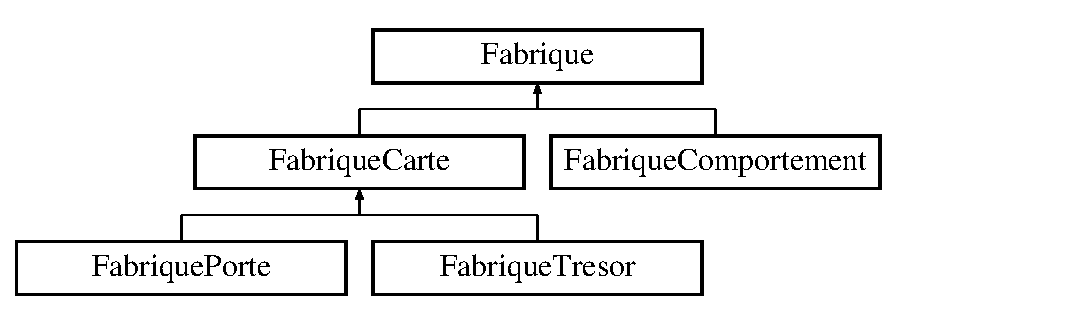
\includegraphics[height=3.000000cm]{class_fabrique}
\end{center}
\end{figure}
\subsection*{Public Member Functions}
\begin{DoxyCompactItemize}
\item 
\hyperlink{class_fabrique_ab3a6fffb52ff91bd94b6355ae104b3fa}{Fabrique} ()
\begin{DoxyCompactList}\small\item\em Constructeur. \end{DoxyCompactList}\item 
virtual \hyperlink{class_fabrique_ac0778fed08ce84fd4f9f8a253a5ad7d5}{$\sim$\-Fabrique} ()
\begin{DoxyCompactList}\small\item\em Destructeur. \end{DoxyCompactList}\item 
virtual std\-::vector$<$ std\-::string $>$ \hyperlink{class_fabrique_a069aadcb4a6e95c87d9421962fa49cb2}{decomp\-String} (std\-::string info)=0
\begin{DoxyCompactList}\small\item\em Découpe la ligne. \end{DoxyCompactList}\end{DoxyCompactItemize}


\subsection{Constructor \& Destructor Documentation}
\hypertarget{class_fabrique_ab3a6fffb52ff91bd94b6355ae104b3fa}{\index{Fabrique@{Fabrique}!Fabrique@{Fabrique}}
\index{Fabrique@{Fabrique}!Fabrique@{Fabrique}}
\subsubsection[{Fabrique}]{\setlength{\rightskip}{0pt plus 5cm}Fabrique\-::\-Fabrique (
\begin{DoxyParamCaption}
{}
\end{DoxyParamCaption}
)}}\label{class_fabrique_ab3a6fffb52ff91bd94b6355ae104b3fa}


Constructeur. 

Constructeur de la classe \hyperlink{class_fabrique}{Fabrique} \hypertarget{class_fabrique_ac0778fed08ce84fd4f9f8a253a5ad7d5}{\index{Fabrique@{Fabrique}!$\sim$\-Fabrique@{$\sim$\-Fabrique}}
\index{$\sim$\-Fabrique@{$\sim$\-Fabrique}!Fabrique@{Fabrique}}
\subsubsection[{$\sim$\-Fabrique}]{\setlength{\rightskip}{0pt plus 5cm}Fabrique\-::$\sim$\-Fabrique (
\begin{DoxyParamCaption}
{}
\end{DoxyParamCaption}
)\hspace{0.3cm}{\ttfamily [virtual]}}}\label{class_fabrique_ac0778fed08ce84fd4f9f8a253a5ad7d5}


Destructeur. 

Destructeur de la classe C\-Player 

\subsection{Member Function Documentation}
\hypertarget{class_fabrique_a069aadcb4a6e95c87d9421962fa49cb2}{\index{Fabrique@{Fabrique}!decomp\-String@{decomp\-String}}
\index{decomp\-String@{decomp\-String}!Fabrique@{Fabrique}}
\subsubsection[{decomp\-String}]{\setlength{\rightskip}{0pt plus 5cm}virtual std\-::vector$<$std\-::string$>$ Fabrique\-::decomp\-String (
\begin{DoxyParamCaption}
\item[{std\-::string}]{info}
\end{DoxyParamCaption}
)\hspace{0.3cm}{\ttfamily [pure virtual]}}}\label{class_fabrique_a069aadcb4a6e95c87d9421962fa49cb2}


Découpe la ligne. 

Methode qui découpe une chaine en liste de chaine.


\begin{DoxyParams}{Parameters}
{\em info} & une chaine de caractere. \\
\hline
\end{DoxyParams}
\begin{DoxyReturn}{Returns}
une liste de chaine de caractere. 
\end{DoxyReturn}


Implemented in \hyperlink{class_fabrique_comportement_a166b586a89e0f86a57202eee119a3dcc}{Fabrique\-Comportement}, and \hyperlink{class_fabrique_carte_a12833e3935bb307640b1cc8307c55c86}{Fabrique\-Carte}.



The documentation for this class was generated from the following files\-:\begin{DoxyCompactItemize}
\item 
\hyperlink{_fabrique_8hpp}{Fabrique.\-hpp}\item 
Fabrique.\-cpp\end{DoxyCompactItemize}

\hypertarget{class_fabrique_carte}{\section{Fabrique\-Carte Class Reference}
\label{class_fabrique_carte}\index{Fabrique\-Carte@{Fabrique\-Carte}}
}
Inheritance diagram for Fabrique\-Carte\-:\begin{figure}[H]
\begin{center}
\leavevmode
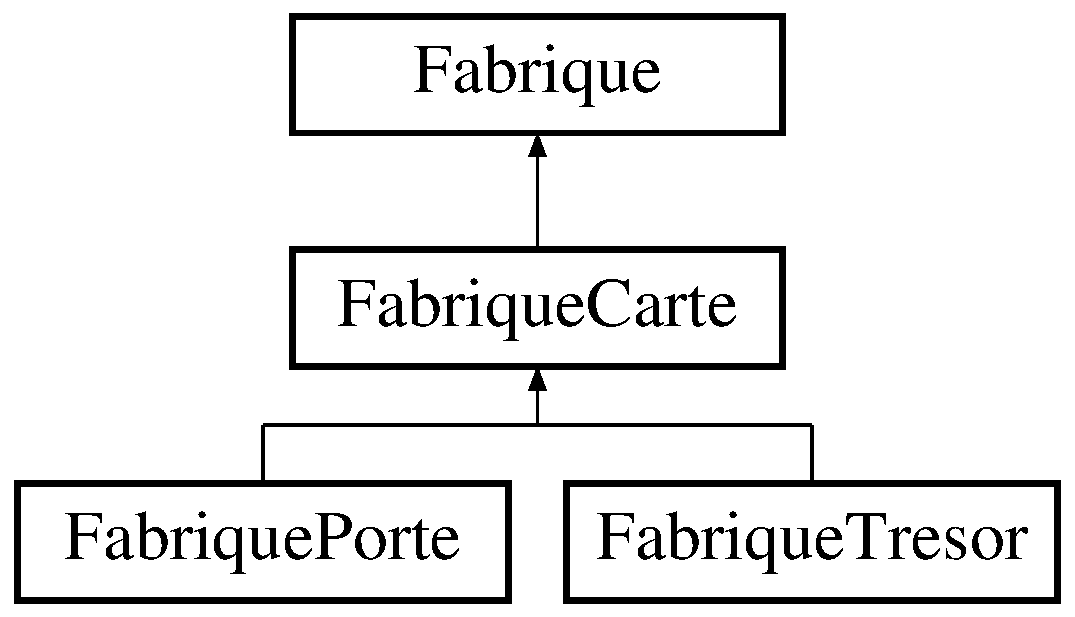
\includegraphics[height=3.000000cm]{class_fabrique_carte}
\end{center}
\end{figure}
\subsection*{Public Member Functions}
\begin{DoxyCompactItemize}
\item 
\hyperlink{class_fabrique_carte_ad7d6eb6e69d966075d7a91c5838d4db5}{Fabrique\-Carte} ()
\begin{DoxyCompactList}\small\item\em Constructeur. \end{DoxyCompactList}\item 
virtual \hyperlink{class_fabrique_carte_a84f2d3be7f193da3abca977a2d588a72}{$\sim$\-Fabrique\-Carte} ()
\begin{DoxyCompactList}\small\item\em Destructeur. \end{DoxyCompactList}\item 
std\-::vector$<$ std\-::string $>$ \hyperlink{class_fabrique_carte_a12833e3935bb307640b1cc8307c55c86}{decomp\-String} (std\-::string info)
\begin{DoxyCompactList}\small\item\em D�coupe la ligne. \end{DoxyCompactList}\item 
\hypertarget{class_fabrique_carte_a2ec2e7701224a6eaaf6ffdc2f108d1d5}{virtual \hyperlink{class_carte}{Carte} $\ast$ {\bfseries fabriquer} (std\-::vector$<$ std\-::string $>$ champs)=0}\label{class_fabrique_carte_a2ec2e7701224a6eaaf6ffdc2f108d1d5}

\end{DoxyCompactItemize}
\subsection*{Protected Attributes}
\begin{DoxyCompactItemize}
\item 
\hypertarget{class_fabrique_carte_ad700917bbe33836b0a86bb1271e28da6}{\hyperlink{class_fabrique_comportement}{Fabrique\-Comportement} $\ast$ {\bfseries comportement}}\label{class_fabrique_carte_ad700917bbe33836b0a86bb1271e28da6}

\end{DoxyCompactItemize}


\subsection{Constructor \& Destructor Documentation}
\hypertarget{class_fabrique_carte_ad7d6eb6e69d966075d7a91c5838d4db5}{\index{Fabrique\-Carte@{Fabrique\-Carte}!Fabrique\-Carte@{Fabrique\-Carte}}
\index{Fabrique\-Carte@{Fabrique\-Carte}!FabriqueCarte@{Fabrique\-Carte}}
\subsubsection[{Fabrique\-Carte}]{\setlength{\rightskip}{0pt plus 5cm}Fabrique\-Carte\-::\-Fabrique\-Carte (
\begin{DoxyParamCaption}
{}
\end{DoxyParamCaption}
)}}\label{class_fabrique_carte_ad7d6eb6e69d966075d7a91c5838d4db5}


Constructeur. 

Constructeur de la classe \hyperlink{class_fabrique_carte}{Fabrique\-Carte} \hypertarget{class_fabrique_carte_a84f2d3be7f193da3abca977a2d588a72}{\index{Fabrique\-Carte@{Fabrique\-Carte}!$\sim$\-Fabrique\-Carte@{$\sim$\-Fabrique\-Carte}}
\index{$\sim$\-Fabrique\-Carte@{$\sim$\-Fabrique\-Carte}!FabriqueCarte@{Fabrique\-Carte}}
\subsubsection[{$\sim$\-Fabrique\-Carte}]{\setlength{\rightskip}{0pt plus 5cm}Fabrique\-Carte\-::$\sim$\-Fabrique\-Carte (
\begin{DoxyParamCaption}
{}
\end{DoxyParamCaption}
)\hspace{0.3cm}{\ttfamily [virtual]}}}\label{class_fabrique_carte_a84f2d3be7f193da3abca977a2d588a72}


Destructeur. 

Destructeur de la classe \hyperlink{class_fabrique_carte}{Fabrique\-Carte} 

\subsection{Member Function Documentation}
\hypertarget{class_fabrique_carte_a12833e3935bb307640b1cc8307c55c86}{\index{Fabrique\-Carte@{Fabrique\-Carte}!decomp\-String@{decomp\-String}}
\index{decomp\-String@{decomp\-String}!FabriqueCarte@{Fabrique\-Carte}}
\subsubsection[{decomp\-String}]{\setlength{\rightskip}{0pt plus 5cm}std\-::vector$<$ std\-::string $>$ Fabrique\-Carte\-::decomp\-String (
\begin{DoxyParamCaption}
\item[{std\-::string}]{info}
\end{DoxyParamCaption}
)\hspace{0.3cm}{\ttfamily [virtual]}}}\label{class_fabrique_carte_a12833e3935bb307640b1cc8307c55c86}


D�coupe la ligne. 

Methode qui d�coupe une chaine en liste de chaine.


\begin{DoxyParams}{Parameters}
{\em info} & une chaine de caractere. \\
\hline
\end{DoxyParams}
\begin{DoxyReturn}{Returns}
une liste de chaine de caractere. 
\end{DoxyReturn}


Implements \hyperlink{class_fabrique_a069aadcb4a6e95c87d9421962fa49cb2}{Fabrique}.



The documentation for this class was generated from the following files\-:\begin{DoxyCompactItemize}
\item 
\hyperlink{_fabrique_carte_8hpp}{Fabrique\-Carte.\-hpp}\item 
Fabrique\-Carte.\-cpp\end{DoxyCompactItemize}

\hypertarget{class_fabrique_comportement}{\section{Fabrique\-Comportement Class Reference}
\label{class_fabrique_comportement}\index{Fabrique\-Comportement@{Fabrique\-Comportement}}
}
Inheritance diagram for Fabrique\-Comportement\-:\begin{figure}[H]
\begin{center}
\leavevmode
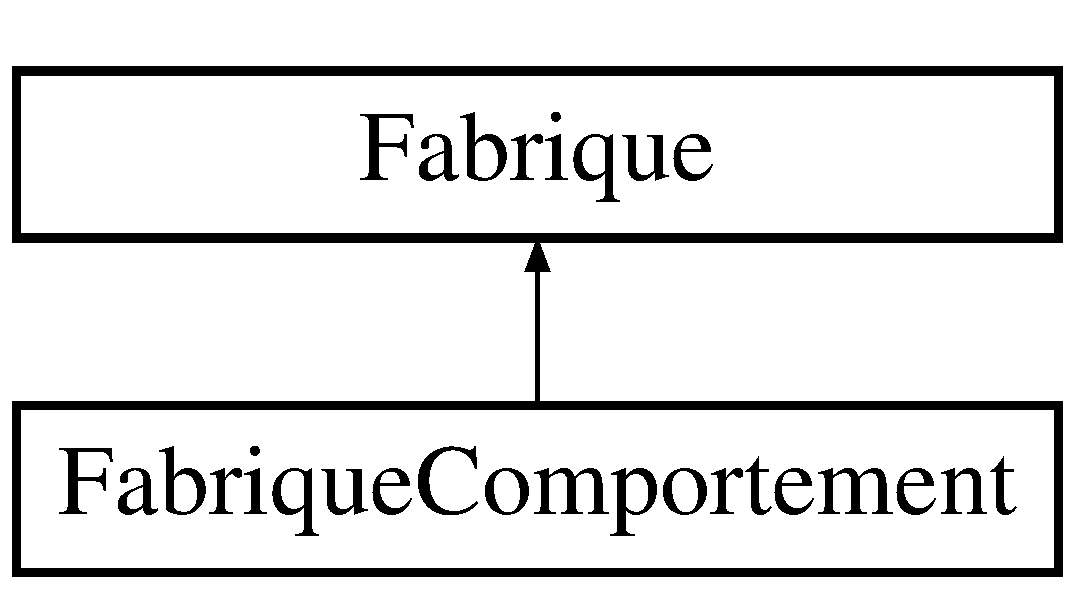
\includegraphics[height=2.000000cm]{class_fabrique_comportement}
\end{center}
\end{figure}
\subsection*{Public Member Functions}
\begin{DoxyCompactItemize}
\item 
\hyperlink{class_fabrique_comportement_a6dbfe3f5ed715a11f74b311625a94cfd}{Fabrique\-Comportement} ()
\begin{DoxyCompactList}\small\item\em Constructeur. \end{DoxyCompactList}\item 
virtual \hyperlink{class_fabrique_comportement_a73b72a29312ca0f16d750bb6ed45f29c}{$\sim$\-Fabrique\-Comportement} ()
\begin{DoxyCompactList}\small\item\em Destructeur. \end{DoxyCompactList}\item 
\hyperlink{class_carte}{Carte} $\ast$ \hyperlink{class_fabrique_comportement_a9fcb07ef95aacd3677bba993fafa084e}{fabriquer} (std\-::vector$<$ std\-::string $>$ champs, \hyperlink{class_carte}{Carte} $\ast$c)
\begin{DoxyCompactList}\small\item\em fabrique une \hyperlink{class_carte}{Carte}. \end{DoxyCompactList}\item 
std\-::vector$<$ std\-::string $>$ \hyperlink{class_fabrique_comportement_a166b586a89e0f86a57202eee119a3dcc}{decomp\-String} (std\-::string info)
\begin{DoxyCompactList}\small\item\em Découpe la ligne. \end{DoxyCompactList}\end{DoxyCompactItemize}


\subsection{Constructor \& Destructor Documentation}
\hypertarget{class_fabrique_comportement_a6dbfe3f5ed715a11f74b311625a94cfd}{\index{Fabrique\-Comportement@{Fabrique\-Comportement}!Fabrique\-Comportement@{Fabrique\-Comportement}}
\index{Fabrique\-Comportement@{Fabrique\-Comportement}!FabriqueComportement@{Fabrique\-Comportement}}
\subsubsection[{Fabrique\-Comportement}]{\setlength{\rightskip}{0pt plus 5cm}Fabrique\-Comportement\-::\-Fabrique\-Comportement (
\begin{DoxyParamCaption}
{}
\end{DoxyParamCaption}
)}}\label{class_fabrique_comportement_a6dbfe3f5ed715a11f74b311625a94cfd}


Constructeur. 

Constructeur de la classe \hyperlink{class_fabrique_comportement}{Fabrique\-Comportement} \hypertarget{class_fabrique_comportement_a73b72a29312ca0f16d750bb6ed45f29c}{\index{Fabrique\-Comportement@{Fabrique\-Comportement}!$\sim$\-Fabrique\-Comportement@{$\sim$\-Fabrique\-Comportement}}
\index{$\sim$\-Fabrique\-Comportement@{$\sim$\-Fabrique\-Comportement}!FabriqueComportement@{Fabrique\-Comportement}}
\subsubsection[{$\sim$\-Fabrique\-Comportement}]{\setlength{\rightskip}{0pt plus 5cm}Fabrique\-Comportement\-::$\sim$\-Fabrique\-Comportement (
\begin{DoxyParamCaption}
{}
\end{DoxyParamCaption}
)\hspace{0.3cm}{\ttfamily [virtual]}}}\label{class_fabrique_comportement_a73b72a29312ca0f16d750bb6ed45f29c}


Destructeur. 

Destructeur de la classe \hyperlink{class_fabrique_comportement}{Fabrique\-Comportement} 

\subsection{Member Function Documentation}
\hypertarget{class_fabrique_comportement_a166b586a89e0f86a57202eee119a3dcc}{\index{Fabrique\-Comportement@{Fabrique\-Comportement}!decomp\-String@{decomp\-String}}
\index{decomp\-String@{decomp\-String}!FabriqueComportement@{Fabrique\-Comportement}}
\subsubsection[{decomp\-String}]{\setlength{\rightskip}{0pt plus 5cm}std\-::vector$<$ std\-::string $>$ Fabrique\-Comportement\-::decomp\-String (
\begin{DoxyParamCaption}
\item[{std\-::string}]{info}
\end{DoxyParamCaption}
)\hspace{0.3cm}{\ttfamily [virtual]}}}\label{class_fabrique_comportement_a166b586a89e0f86a57202eee119a3dcc}


Découpe la ligne. 

Methode qui découpe une chaine en liste de chaine.


\begin{DoxyParams}{Parameters}
{\em info} & une chaine de caractere. \\
\hline
\end{DoxyParams}
\begin{DoxyReturn}{Returns}
une liste de chaine de caractere. 
\end{DoxyReturn}


Implements \hyperlink{class_fabrique_a069aadcb4a6e95c87d9421962fa49cb2}{Fabrique}.

\hypertarget{class_fabrique_comportement_a9fcb07ef95aacd3677bba993fafa084e}{\index{Fabrique\-Comportement@{Fabrique\-Comportement}!fabriquer@{fabriquer}}
\index{fabriquer@{fabriquer}!FabriqueComportement@{Fabrique\-Comportement}}
\subsubsection[{fabriquer}]{\setlength{\rightskip}{0pt plus 5cm}{\bf Carte} $\ast$ Fabrique\-Comportement\-::fabriquer (
\begin{DoxyParamCaption}
\item[{std\-::vector$<$ std\-::string $>$}]{champs, }
\item[{{\bf Carte} $\ast$}]{c}
\end{DoxyParamCaption}
)}}\label{class_fabrique_comportement_a9fcb07ef95aacd3677bba993fafa084e}


fabrique une \hyperlink{class_carte}{Carte}. 

Methode qui retourne la \hyperlink{class_carte}{Carte} décoré avec les informations de la liste données en parametres.


\begin{DoxyParams}{Parameters}
{\em champs} & \-: liste de chaine de caractere contenant les informations. \\
\hline
{\em c} & \-: \hyperlink{class_carte}{Carte} a décorer. \\
\hline
\end{DoxyParams}
\begin{DoxyReturn}{Returns}
une \hyperlink{class_carte}{Carte} avec un comportement. 
\end{DoxyReturn}


The documentation for this class was generated from the following files\-:\begin{DoxyCompactItemize}
\item 
\hyperlink{_fabrique_comportement_8hpp}{Fabrique\-Comportement.\-hpp}\item 
Fabrique\-Comportement.\-cpp\end{DoxyCompactItemize}

\hypertarget{class_fabrique_porte}{\section{Fabrique\-Porte Class Reference}
\label{class_fabrique_porte}\index{Fabrique\-Porte@{Fabrique\-Porte}}
}
Inheritance diagram for Fabrique\-Porte\-:\begin{figure}[H]
\begin{center}
\leavevmode
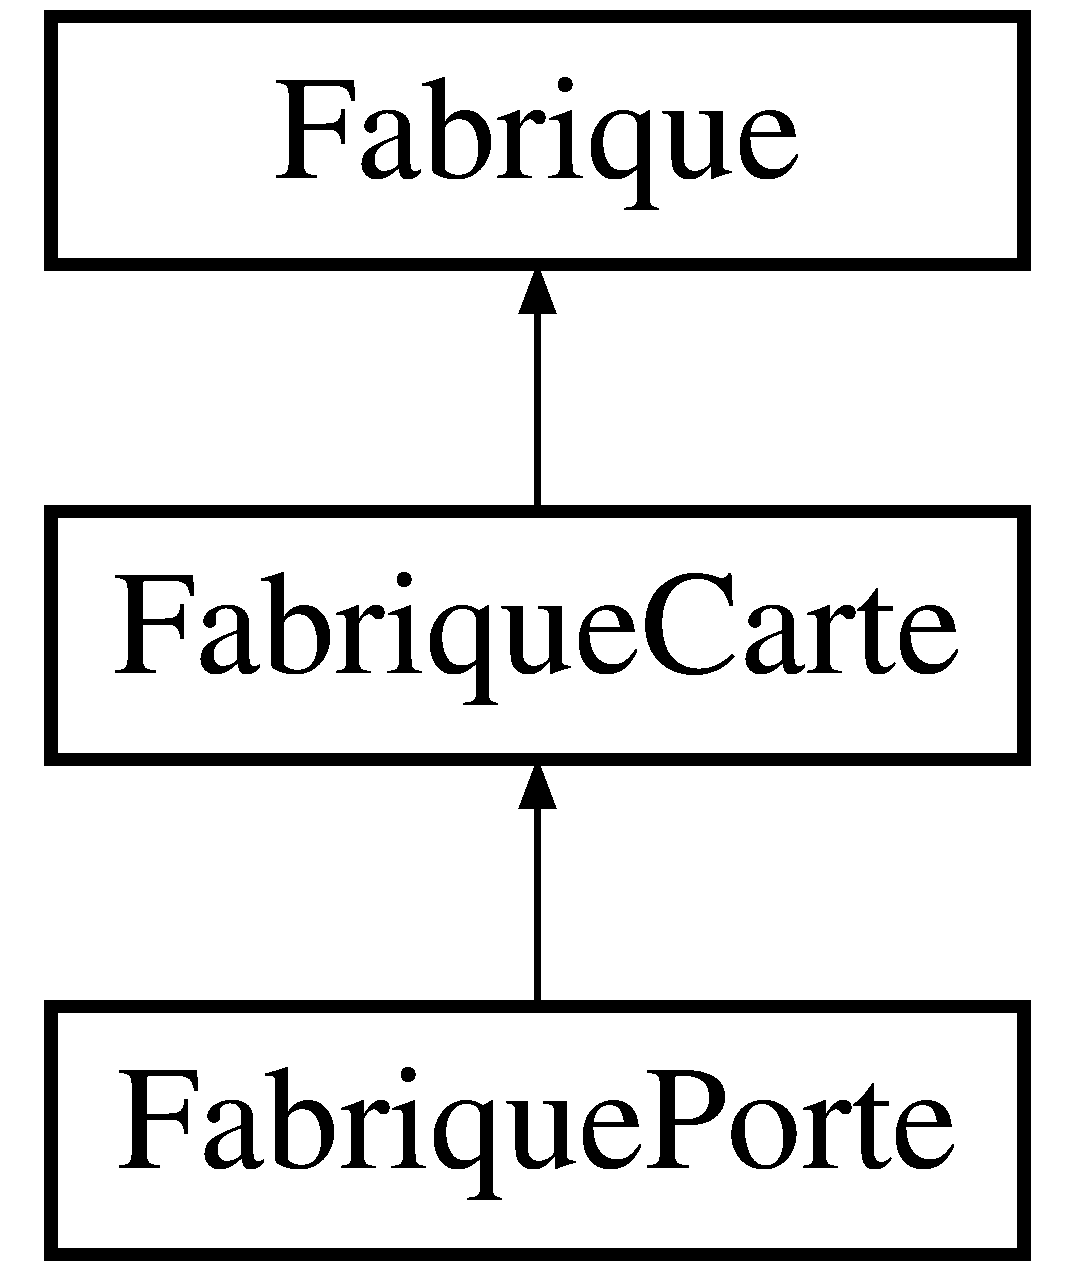
\includegraphics[height=3.000000cm]{class_fabrique_porte}
\end{center}
\end{figure}
\subsection*{Public Member Functions}
\begin{DoxyCompactItemize}
\item 
\hyperlink{class_fabrique_porte_a99f6ef2c1d0e890c6b677f8c876f26e2}{Fabrique\-Porte} ()
\begin{DoxyCompactList}\small\item\em Constructeur. \end{DoxyCompactList}\item 
\hyperlink{class_fabrique_porte_ab1db4cd42e6a6a4ac4e10f0a46f7f516}{$\sim$\-Fabrique\-Porte} ()
\begin{DoxyCompactList}\small\item\em Destructeur. \end{DoxyCompactList}\item 
\hypertarget{class_fabrique_porte_a7a80270fc14a552ea38c5e12d19d46e8}{\hyperlink{class_carte}{Carte} $\ast$ {\bfseries fabriquer} (vector$<$ string $>$ champs)}\label{class_fabrique_porte_a7a80270fc14a552ea38c5e12d19d46e8}

\end{DoxyCompactItemize}
\subsection*{Additional Inherited Members}


\subsection{Constructor \& Destructor Documentation}
\hypertarget{class_fabrique_porte_a99f6ef2c1d0e890c6b677f8c876f26e2}{\index{Fabrique\-Porte@{Fabrique\-Porte}!Fabrique\-Porte@{Fabrique\-Porte}}
\index{Fabrique\-Porte@{Fabrique\-Porte}!FabriquePorte@{Fabrique\-Porte}}
\subsubsection[{Fabrique\-Porte}]{\setlength{\rightskip}{0pt plus 5cm}Fabrique\-Porte\-::\-Fabrique\-Porte (
\begin{DoxyParamCaption}
{}
\end{DoxyParamCaption}
)}}\label{class_fabrique_porte_a99f6ef2c1d0e890c6b677f8c876f26e2}


Constructeur. 

Constructeur de la classe \hyperlink{class_fabrique}{Fabrique} \hypertarget{class_fabrique_porte_ab1db4cd42e6a6a4ac4e10f0a46f7f516}{\index{Fabrique\-Porte@{Fabrique\-Porte}!$\sim$\-Fabrique\-Porte@{$\sim$\-Fabrique\-Porte}}
\index{$\sim$\-Fabrique\-Porte@{$\sim$\-Fabrique\-Porte}!FabriquePorte@{Fabrique\-Porte}}
\subsubsection[{$\sim$\-Fabrique\-Porte}]{\setlength{\rightskip}{0pt plus 5cm}Fabrique\-Porte\-::$\sim$\-Fabrique\-Porte (
\begin{DoxyParamCaption}
{}
\end{DoxyParamCaption}
)}}\label{class_fabrique_porte_ab1db4cd42e6a6a4ac4e10f0a46f7f516}


Destructeur. 

Destructeur de la classe \hyperlink{class_fabrique_carte}{Fabrique\-Carte} 

The documentation for this class was generated from the following files\-:\begin{DoxyCompactItemize}
\item 
\hyperlink{_fabrique_porte_8hpp}{Fabrique\-Porte.\-hpp}\item 
Fabrique\-Porte.\-cpp\end{DoxyCompactItemize}

\hypertarget{class_fabrique_tresor}{\section{Fabrique\-Tresor Class Reference}
\label{class_fabrique_tresor}\index{Fabrique\-Tresor@{Fabrique\-Tresor}}
}
Inheritance diagram for Fabrique\-Tresor\-:\begin{figure}[H]
\begin{center}
\leavevmode
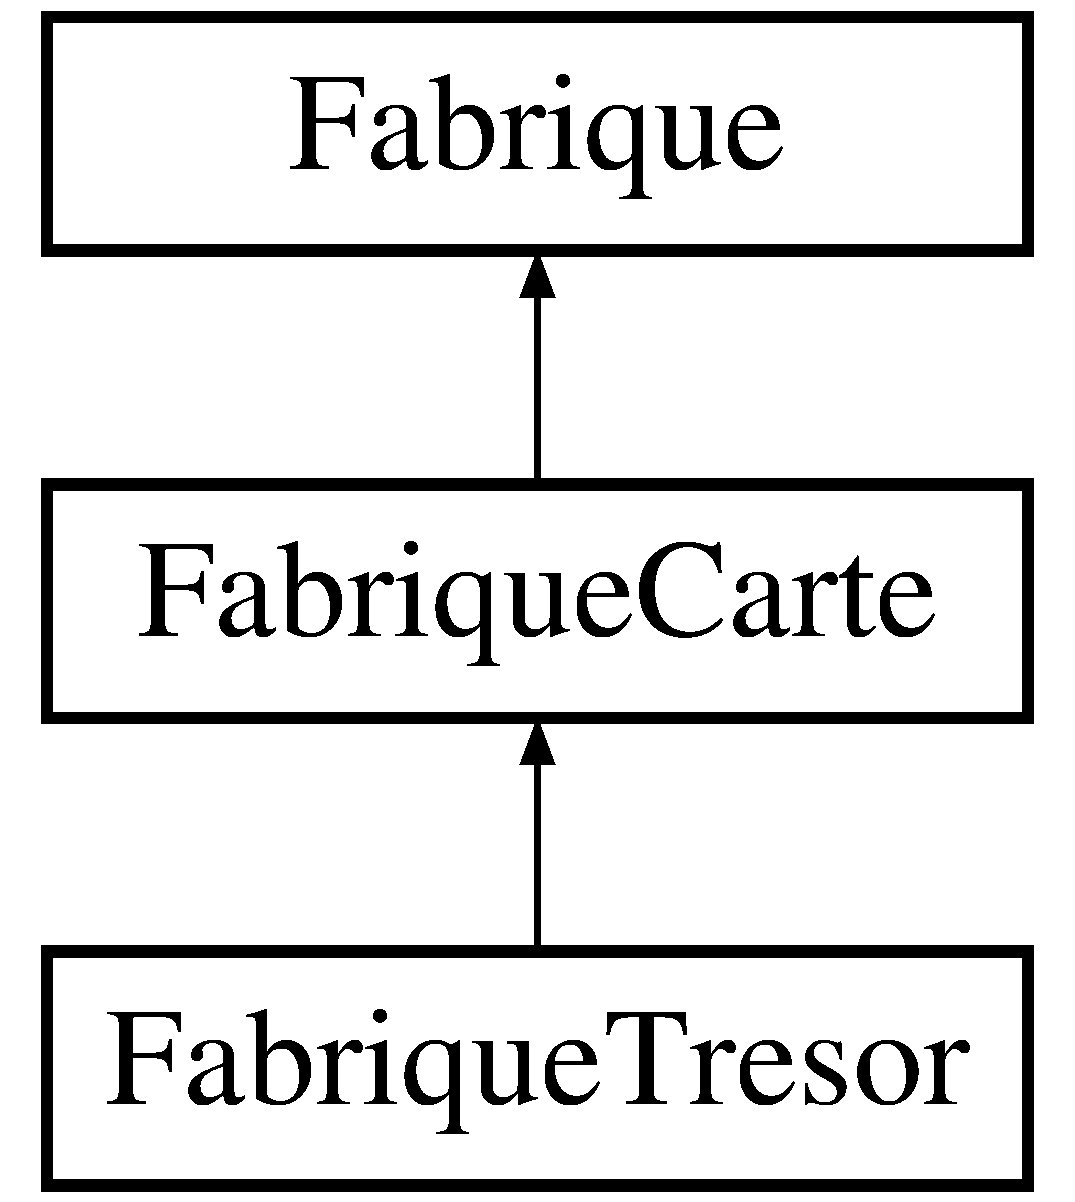
\includegraphics[height=3.000000cm]{class_fabrique_tresor}
\end{center}
\end{figure}
\subsection*{Public Member Functions}
\begin{DoxyCompactItemize}
\item 
\hyperlink{class_fabrique_tresor_a589e38fdb2d1f1254028ec0611c5e160}{Fabrique\-Tresor} ()
\begin{DoxyCompactList}\small\item\em Constructeur. \end{DoxyCompactList}\item 
\hyperlink{class_fabrique_tresor_a3160984c18eb8a9f78df8d4751551f3c}{$\sim$\-Fabrique\-Tresor} ()
\begin{DoxyCompactList}\small\item\em Destructeur. \end{DoxyCompactList}\item 
\hypertarget{class_fabrique_tresor_a99902ef13463275657fb372688991db8}{\hyperlink{class_carte}{Carte} $\ast$ {\bfseries fabriquer} (std\-::vector$<$ std\-::string $>$ champs)}\label{class_fabrique_tresor_a99902ef13463275657fb372688991db8}

\end{DoxyCompactItemize}
\subsection*{Additional Inherited Members}


\subsection{Constructor \& Destructor Documentation}
\hypertarget{class_fabrique_tresor_a589e38fdb2d1f1254028ec0611c5e160}{\index{Fabrique\-Tresor@{Fabrique\-Tresor}!Fabrique\-Tresor@{Fabrique\-Tresor}}
\index{Fabrique\-Tresor@{Fabrique\-Tresor}!FabriqueTresor@{Fabrique\-Tresor}}
\subsubsection[{Fabrique\-Tresor}]{\setlength{\rightskip}{0pt plus 5cm}Fabrique\-Tresor\-::\-Fabrique\-Tresor (
\begin{DoxyParamCaption}
{}
\end{DoxyParamCaption}
)}}\label{class_fabrique_tresor_a589e38fdb2d1f1254028ec0611c5e160}


Constructeur. 

Constructeur de la classe \hyperlink{class_fabrique_tresor}{Fabrique\-Tresor} \hypertarget{class_fabrique_tresor_a3160984c18eb8a9f78df8d4751551f3c}{\index{Fabrique\-Tresor@{Fabrique\-Tresor}!$\sim$\-Fabrique\-Tresor@{$\sim$\-Fabrique\-Tresor}}
\index{$\sim$\-Fabrique\-Tresor@{$\sim$\-Fabrique\-Tresor}!FabriqueTresor@{Fabrique\-Tresor}}
\subsubsection[{$\sim$\-Fabrique\-Tresor}]{\setlength{\rightskip}{0pt plus 5cm}Fabrique\-Tresor\-::$\sim$\-Fabrique\-Tresor (
\begin{DoxyParamCaption}
{}
\end{DoxyParamCaption}
)}}\label{class_fabrique_tresor_a3160984c18eb8a9f78df8d4751551f3c}


Destructeur. 

Destructeur de la classe \hyperlink{class_fabrique_tresor}{Fabrique\-Tresor} 

The documentation for this class was generated from the following files\-:\begin{DoxyCompactItemize}
\item 
\hyperlink{_fabrique_tresor_8hpp}{Fabrique\-Tresor.\-hpp}\item 
Fabrique\-Tresor.\-cpp\end{DoxyCompactItemize}

\hypertarget{class_fin_tour}{\section{Fin\-Tour Class Reference}
\label{class_fin_tour}\index{Fin\-Tour@{Fin\-Tour}}
}
Inheritance diagram for Fin\-Tour\-:\begin{figure}[H]
\begin{center}
\leavevmode
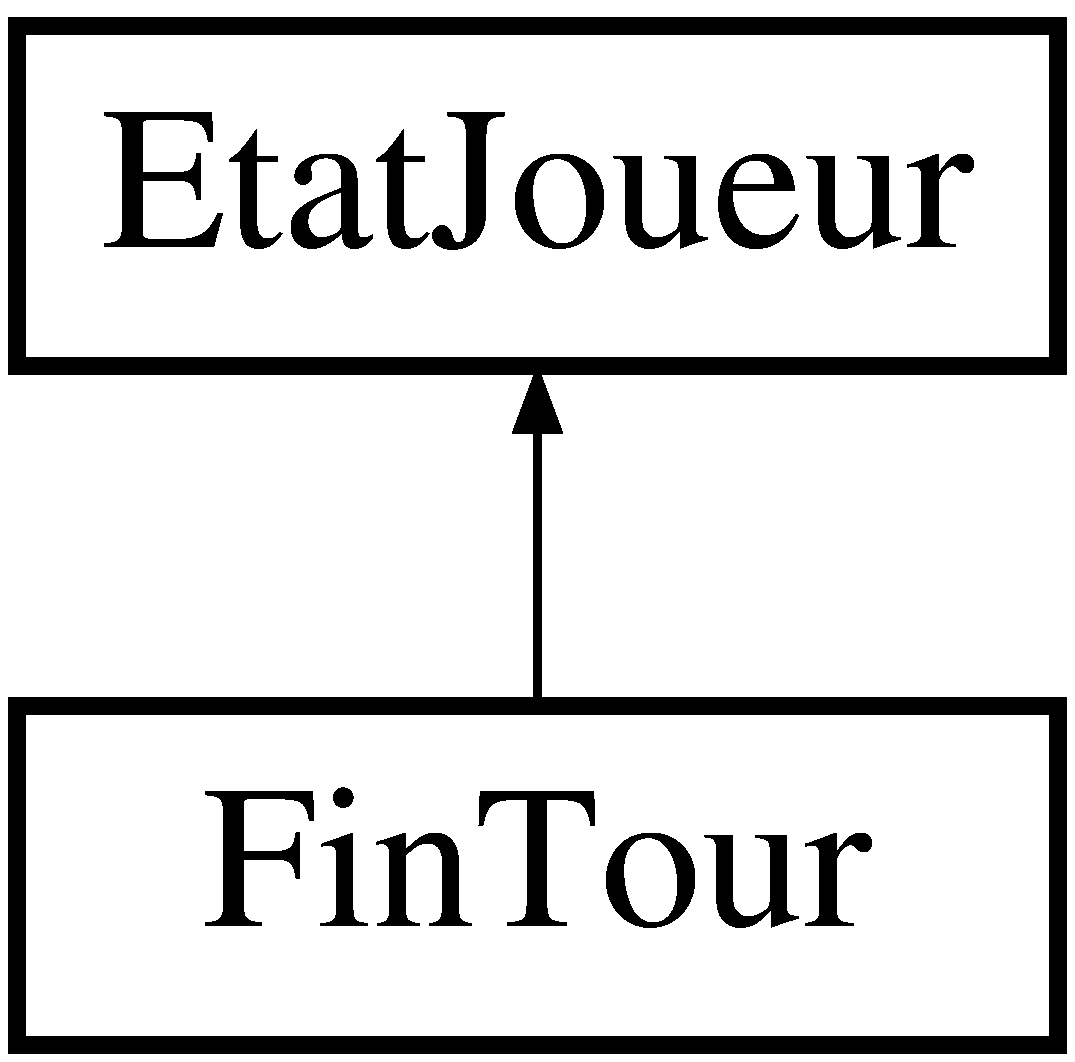
\includegraphics[height=2.000000cm]{class_fin_tour}
\end{center}
\end{figure}
\subsection*{Public Member Functions}
\begin{DoxyCompactItemize}
\item 
\hyperlink{class_fin_tour_ab8aa4db87a4508d466864482b33778db}{Fin\-Tour} (\hyperlink{class_joueur}{Joueur} $\ast$t)
\begin{DoxyCompactList}\small\item\em Constructeur de \hyperlink{class_fin_tour}{Fin\-Tour}. \end{DoxyCompactList}\item 
\hypertarget{class_fin_tour_a7905caca6049a1beb61c93b609914202}{virtual \hyperlink{class_fin_tour_a7905caca6049a1beb61c93b609914202}{$\sim$\-Fin\-Tour} ()}\label{class_fin_tour_a7905caca6049a1beb61c93b609914202}

\begin{DoxyCompactList}\small\item\em Destructeur de \hyperlink{class_fin_tour}{Fin\-Tour}. \end{DoxyCompactList}\item 
\hypertarget{class_fin_tour_a9d435d089d1afe6aa9170ac21389dc4c}{void \hyperlink{class_fin_tour_a9d435d089d1afe6aa9170ac21389dc4c}{finir\-Tour} ()}\label{class_fin_tour_a9d435d089d1afe6aa9170ac21389dc4c}

\begin{DoxyCompactList}\small\item\em Permet au joueur de finir son tour. \end{DoxyCompactList}\item 
void \hyperlink{class_fin_tour_abb40077b94a4b3e345b41299deb6266b}{defausser\-Carte} (\hyperlink{class_carte}{Carte} $\ast$c)
\begin{DoxyCompactList}\small\item\em Permet au joueur de défausser des cartes. \end{DoxyCompactList}\item 
void \hyperlink{class_fin_tour_a6b217f7a319c9daba98722b86b30da66}{changer\-Race} (\hyperlink{class_carte}{Carte} $\ast$r)
\begin{DoxyCompactList}\small\item\em Permet au joueur de changer de race. \end{DoxyCompactList}\item 
void \hyperlink{class_fin_tour_a14304d88c8b344c35cd44fe609c499b6}{pose\-Equipement} (\hyperlink{class_carte}{Carte} $\ast$e)
\begin{DoxyCompactList}\small\item\em Permet au joueur de poser un équipement. \end{DoxyCompactList}\item 
void \hyperlink{class_fin_tour_a08a9ac7c490c13d6f4b116a55abdad86}{equiper} (\hyperlink{class_carte}{Carte} $\ast$e)
\begin{DoxyCompactList}\small\item\em Permet au joueur d'équiper un équipement. \end{DoxyCompactList}\item 
void \hyperlink{class_fin_tour_a526c160be39842a8d61c753ee5f3e6bf}{poser\-Malediction} (\hyperlink{class_joueur}{Joueur} $\ast$cible, \hyperlink{class_carte}{Carte} $\ast$m)
\begin{DoxyCompactList}\small\item\em Permet au joueur de poser une malédiction contre un autre joueur. \end{DoxyCompactList}\end{DoxyCompactItemize}
\subsection*{Additional Inherited Members}


\subsection{Constructor \& Destructor Documentation}
\hypertarget{class_fin_tour_ab8aa4db87a4508d466864482b33778db}{\index{Fin\-Tour@{Fin\-Tour}!Fin\-Tour@{Fin\-Tour}}
\index{Fin\-Tour@{Fin\-Tour}!FinTour@{Fin\-Tour}}
\subsubsection[{Fin\-Tour}]{\setlength{\rightskip}{0pt plus 5cm}Fin\-Tour\-::\-Fin\-Tour (
\begin{DoxyParamCaption}
\item[{{\bf Joueur} $\ast$}]{t}
\end{DoxyParamCaption}
)}}\label{class_fin_tour_ab8aa4db87a4508d466864482b33778db}


Constructeur de \hyperlink{class_fin_tour}{Fin\-Tour}. 


\begin{DoxyParams}{Parameters}
{\em t} & \hyperlink{class_joueur}{Joueur} dont l'état doit être géré \\
\hline
\end{DoxyParams}


\subsection{Member Function Documentation}
\hypertarget{class_fin_tour_a6b217f7a319c9daba98722b86b30da66}{\index{Fin\-Tour@{Fin\-Tour}!changer\-Race@{changer\-Race}}
\index{changer\-Race@{changer\-Race}!FinTour@{Fin\-Tour}}
\subsubsection[{changer\-Race}]{\setlength{\rightskip}{0pt plus 5cm}void Fin\-Tour\-::changer\-Race (
\begin{DoxyParamCaption}
\item[{{\bf Carte} $\ast$}]{r}
\end{DoxyParamCaption}
)\hspace{0.3cm}{\ttfamily [virtual]}}}\label{class_fin_tour_a6b217f7a319c9daba98722b86b30da66}


Permet au joueur de changer de race. 


\begin{DoxyParams}{Parameters}
{\em r} & nouvelle race \\
\hline
\end{DoxyParams}


Reimplemented from \hyperlink{class_etat_joueur_ad60942aa96f0bfb05771f787964887fe}{Etat\-Joueur}.

\hypertarget{class_fin_tour_abb40077b94a4b3e345b41299deb6266b}{\index{Fin\-Tour@{Fin\-Tour}!defausser\-Carte@{defausser\-Carte}}
\index{defausser\-Carte@{defausser\-Carte}!FinTour@{Fin\-Tour}}
\subsubsection[{defausser\-Carte}]{\setlength{\rightskip}{0pt plus 5cm}void Fin\-Tour\-::defausser\-Carte (
\begin{DoxyParamCaption}
\item[{{\bf Carte} $\ast$}]{c}
\end{DoxyParamCaption}
)\hspace{0.3cm}{\ttfamily [virtual]}}}\label{class_fin_tour_abb40077b94a4b3e345b41299deb6266b}


Permet au joueur de défausser des cartes. 


\begin{DoxyParams}{Parameters}
{\em c} & \hyperlink{class_carte}{Carte} à défausser \\
\hline
\end{DoxyParams}


Reimplemented from \hyperlink{class_etat_joueur_a64113ef4494fa9acb088e3d125378735}{Etat\-Joueur}.

\hypertarget{class_fin_tour_a08a9ac7c490c13d6f4b116a55abdad86}{\index{Fin\-Tour@{Fin\-Tour}!equiper@{equiper}}
\index{equiper@{equiper}!FinTour@{Fin\-Tour}}
\subsubsection[{equiper}]{\setlength{\rightskip}{0pt plus 5cm}void Fin\-Tour\-::equiper (
\begin{DoxyParamCaption}
\item[{{\bf Carte} $\ast$}]{e}
\end{DoxyParamCaption}
)\hspace{0.3cm}{\ttfamily [virtual]}}}\label{class_fin_tour_a08a9ac7c490c13d6f4b116a55abdad86}


Permet au joueur d'équiper un équipement. 


\begin{DoxyParams}{Parameters}
{\em e} & equipement à équiper \\
\hline
\end{DoxyParams}


Reimplemented from \hyperlink{class_etat_joueur_a2d975d2cd1163a43d6f0002c1f9943e9}{Etat\-Joueur}.

\hypertarget{class_fin_tour_a14304d88c8b344c35cd44fe609c499b6}{\index{Fin\-Tour@{Fin\-Tour}!pose\-Equipement@{pose\-Equipement}}
\index{pose\-Equipement@{pose\-Equipement}!FinTour@{Fin\-Tour}}
\subsubsection[{pose\-Equipement}]{\setlength{\rightskip}{0pt plus 5cm}void Fin\-Tour\-::pose\-Equipement (
\begin{DoxyParamCaption}
\item[{{\bf Carte} $\ast$}]{e}
\end{DoxyParamCaption}
)\hspace{0.3cm}{\ttfamily [virtual]}}}\label{class_fin_tour_a14304d88c8b344c35cd44fe609c499b6}


Permet au joueur de poser un équipement. 


\begin{DoxyParams}{Parameters}
{\em e} & equipement à poser \\
\hline
\end{DoxyParams}


Reimplemented from \hyperlink{class_etat_joueur_a7d3b72dd7a93a787dcea00d606e9eec2}{Etat\-Joueur}.

\hypertarget{class_fin_tour_a526c160be39842a8d61c753ee5f3e6bf}{\index{Fin\-Tour@{Fin\-Tour}!poser\-Malediction@{poser\-Malediction}}
\index{poser\-Malediction@{poser\-Malediction}!FinTour@{Fin\-Tour}}
\subsubsection[{poser\-Malediction}]{\setlength{\rightskip}{0pt plus 5cm}void Fin\-Tour\-::poser\-Malediction (
\begin{DoxyParamCaption}
\item[{{\bf Joueur} $\ast$}]{cible, }
\item[{{\bf Carte} $\ast$}]{m}
\end{DoxyParamCaption}
)\hspace{0.3cm}{\ttfamily [virtual]}}}\label{class_fin_tour_a526c160be39842a8d61c753ee5f3e6bf}


Permet au joueur de poser une malédiction contre un autre joueur. 


\begin{DoxyParams}{Parameters}
{\em cible} & cible de la malédiction \\
\hline
{\em m} & \hyperlink{class_malediction}{Malediction} à poser \\
\hline
\end{DoxyParams}


Reimplemented from \hyperlink{class_etat_joueur_a6895655263daefa056c3ee11f716cc28}{Etat\-Joueur}.



The documentation for this class was generated from the following files\-:\begin{DoxyCompactItemize}
\item 
\hyperlink{_fin_tour_8hpp}{Fin\-Tour.\-hpp}\item 
\hyperlink{_fin_tour_8cpp}{Fin\-Tour.\-cpp}\end{DoxyCompactItemize}

\hypertarget{class_joueur}{\section{Joueur Class Reference}
\label{class_joueur}\index{Joueur@{Joueur}}
}
Inheritance diagram for Joueur\-:\begin{figure}[H]
\begin{center}
\leavevmode
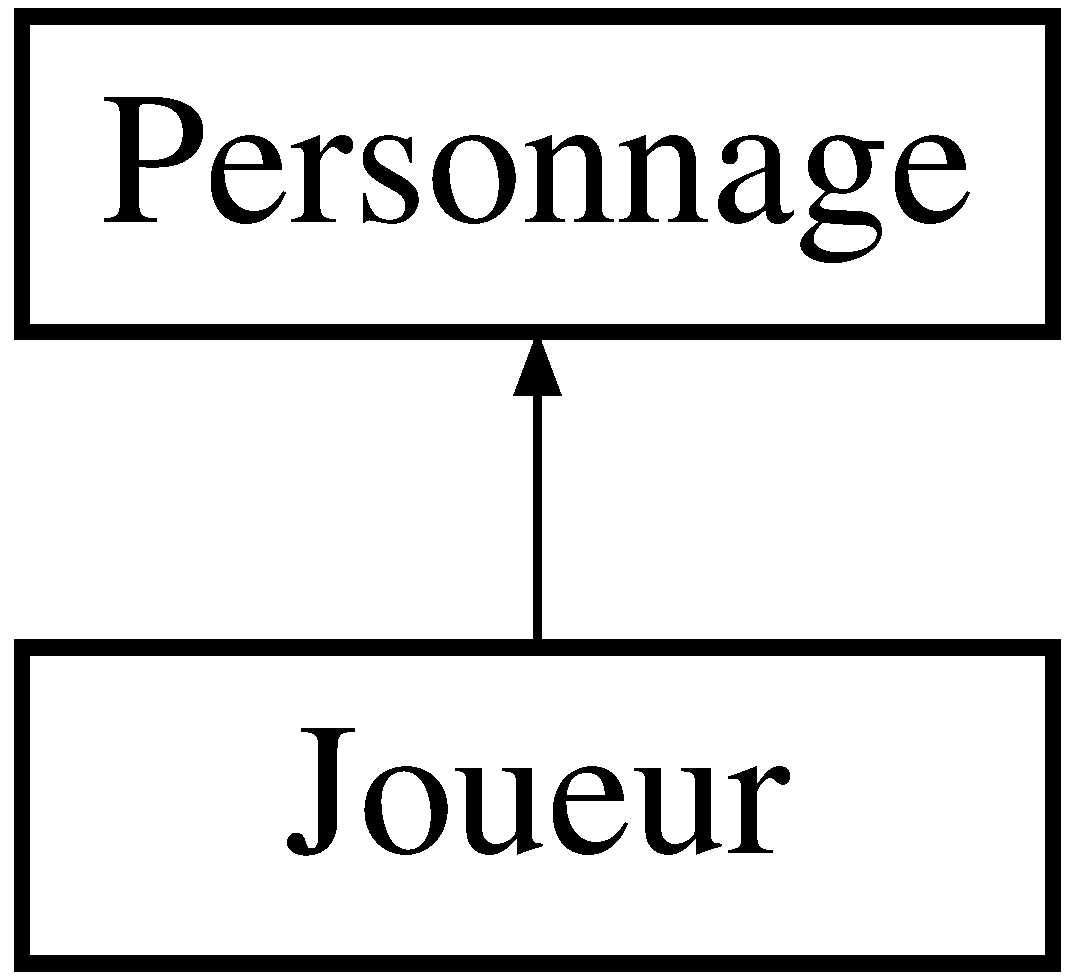
\includegraphics[height=2.000000cm]{class_joueur}
\end{center}
\end{figure}
\subsection*{Public Member Functions}
\begin{DoxyCompactItemize}
\item 
\hyperlink{class_joueur_a222b3b71c83c1815f9a3e001cad97f00}{Joueur} (\hyperlink{class_munchkin}{Munchkin} $\ast$j, int i, \hyperlink{class_race}{Race} $\ast$r)
\begin{DoxyCompactList}\small\item\em Constructeur de \hyperlink{class_joueur}{Joueur}. \end{DoxyCompactList}\item 
\hypertarget{class_joueur_a9fb594f755601ee77ce5884c4c0861f3}{\hyperlink{class_joueur_a9fb594f755601ee77ce5884c4c0861f3}{$\sim$\-Joueur} ()}\label{class_joueur_a9fb594f755601ee77ce5884c4c0861f3}

\begin{DoxyCompactList}\small\item\em Destructeur de \hyperlink{class_joueur}{Joueur}. \end{DoxyCompactList}\item 
\hypertarget{class_joueur_a921d6899073c02644def22d7ef63bcca}{void \hyperlink{class_joueur_a921d6899073c02644def22d7ef63bcca}{afficher} ()}\label{class_joueur_a921d6899073c02644def22d7ef63bcca}

\begin{DoxyCompactList}\small\item\em Affichage des caract�ristiques du joueur. \end{DoxyCompactList}\item 
void \hyperlink{class_joueur_a420c6cf0371d2285570d5ac32b80ebed}{defausser} (\hyperlink{class_carte}{Carte} $\ast$c)
\begin{DoxyCompactList}\small\item\em Permet au joueur de d�fausser une carte. \end{DoxyCompactList}\item 
\hypertarget{class_joueur_a915440670ca5f746c3b70b6f9e623b50}{void \hyperlink{class_joueur_a915440670ca5f746c3b70b6f9e623b50}{fin\-Tour} ()}\label{class_joueur_a915440670ca5f746c3b70b6f9e623b50}

\begin{DoxyCompactList}\small\item\em Permet au joueur de terminer son tour. \end{DoxyCompactList}\item 
void \hyperlink{class_joueur_ad147d4d3d8a56fa600511d3f0aee2410}{equiper\-Equipement} (\hyperlink{class_carte}{Carte} $\ast$e)
\begin{DoxyCompactList}\small\item\em Permet au joueur d'�quiper un equipement. \end{DoxyCompactList}\item 
void \hyperlink{class_joueur_a2bbd462f3d8c0b869f704bce7f9f3d76}{equiper\-Couvre\-Chef} (\hyperlink{class_carte}{Carte} $\ast$c)
\begin{DoxyCompactList}\small\item\em Permet au joueur d'�quiper un \hyperlink{class_couvre_chef}{Couvre\-Chef}. \end{DoxyCompactList}\item 
void \hyperlink{class_joueur_a4a4deded62ce21efad2cf65f482a4eec}{equiper1\-Main} (\hyperlink{class_carte}{Carte} $\ast$m)
\begin{DoxyCompactList}\small\item\em Permet au joueur d'�quiper un objet 1 main. \end{DoxyCompactList}\item 
void \hyperlink{class_joueur_abaec518c206959c4266b1434aa76e644}{equiper2\-Main} (\hyperlink{class_carte}{Carte} $\ast$m)
\begin{DoxyCompactList}\small\item\em Permet au joueur d'�quiper un objet 2 mains. \end{DoxyCompactList}\item 
void \hyperlink{class_joueur_a21fe941d1d4a440545c793369d189987}{equiper\-Armure} (\hyperlink{class_carte}{Carte} $\ast$a)
\begin{DoxyCompactList}\small\item\em Permet au joueur d'�quiper une armure. \end{DoxyCompactList}\item 
void \hyperlink{class_joueur_a108ece9c4dc467cc7b930c57e4fc3017}{equiper\-Chaussure} (\hyperlink{class_carte}{Carte} $\ast$c)
\begin{DoxyCompactList}\small\item\em Permet au joueur d'�quiper des chaussures. \end{DoxyCompactList}\item 
void \hyperlink{class_joueur_a08d1ede84a9b877143571a0ec3e5f6d4}{set\-Nb\-Cartes\-Main} (int n)
\begin{DoxyCompactList}\small\item\em Change la valeur du nombre max de cartes en main. \end{DoxyCompactList}\item 
int \hyperlink{class_joueur_a384452fa155649674af4f34e9e0aa5b3}{get\-Nb\-Cartes\-Main} ()
\begin{DoxyCompactList}\small\item\em Renvoie la valeur du nombre max de cartes en main. \end{DoxyCompactList}\item 
void \hyperlink{class_joueur_a771da66d60d4f6bab21b2f1a0bbbc0e1}{set\-Val\-Deguerpir} (int val)
\begin{DoxyCompactList}\small\item\em Change la valeur du bonus pour deguerpir. \end{DoxyCompactList}\item 
int \hyperlink{class_joueur_aa5eff2695529b5faad48c5abbd636f92}{get\-Val\-Deguerpir} ()
\begin{DoxyCompactList}\small\item\em Renvoie la valeur du bonus pour deguerpir. \end{DoxyCompactList}\item 
\hypertarget{class_joueur_ad62a55e43495b46e5e3c5696b051d53e}{\hyperlink{class_carte}{Carte} $\ast$ {\bfseries get\-Race} ()}\label{class_joueur_ad62a55e43495b46e5e3c5696b051d53e}

\item 
void \hyperlink{class_joueur_a76098559d08040a1e689c6ae7171cf7f}{set\-Race} (\hyperlink{class_carte}{Carte} $\ast$r)
\begin{DoxyCompactList}\small\item\em Change la race du joueur. \end{DoxyCompactList}\item 
int \hyperlink{class_joueur_a344107187c8ff4cdcf133af7e2e2c794}{get\-Id} ()
\begin{DoxyCompactList}\small\item\em Renvoie l'identifiant du joueur. \end{DoxyCompactList}\item 
void \hyperlink{class_joueur_a030c7b6aeb49715647b7e81657090964}{set\-Etat} (\hyperlink{class_etat_joueur}{Etat\-Joueur} $\ast$e)
\begin{DoxyCompactList}\small\item\em Change l'�tat du joueur. \end{DoxyCompactList}\item 
\hyperlink{class_etat_joueur}{Etat\-Joueur} $\ast$ \hyperlink{class_joueur_aadb613c0cb97f4dc944ce0e036f9a0c7}{get\-Etat} ()
\begin{DoxyCompactList}\small\item\em Renvoie l'�tat du joueur. \end{DoxyCompactList}\item 
\hyperlink{class_debut_tour}{Debut\-Tour} $\ast$ \hyperlink{class_joueur_a2a67be62e5d871e4e30800ca7724b661}{get\-Debut} ()
\begin{DoxyCompactList}\small\item\em Renvoie l'�tat debut. \end{DoxyCompactList}\item 
\hyperlink{class_ouvrir_porte}{Ouvrir\-Porte} $\ast$ \hyperlink{class_joueur_a44305d470cb6294335ae11349e44bcaa}{get\-Ouvrir\-La\-Porte} ()
\begin{DoxyCompactList}\small\item\em Renvoie l'�tat ouvrir\-La\-Porte. \end{DoxyCompactList}\item 
\hyperlink{class_bagarre}{Bagarre} $\ast$ \hyperlink{class_joueur_a231ddeacc9c7c0d35499a9608eafe4fa}{get\-Bagarre} ()
\begin{DoxyCompactList}\small\item\em Renvoie l'�tat bagarre. \end{DoxyCompactList}\item 
\hyperlink{class_fin_tour}{Fin\-Tour} $\ast$ \hyperlink{class_joueur_acfbf773dd8dc773e34d7b11c24a98b9a}{get\-Fin} ()
\begin{DoxyCompactList}\small\item\em Renvoie l'�tat fin. \end{DoxyCompactList}\item 
\hyperlink{class_attente}{Attente} $\ast$ \hyperlink{class_joueur_acab52513b71595b5bd34acb7e166d457}{get\-Attente} ()
\begin{DoxyCompactList}\small\item\em Renvoie l'�tat attente. \end{DoxyCompactList}\item 
vector$<$ \hyperlink{class_carte}{Carte} $\ast$ $>$ \& \hyperlink{class_joueur_acb4761028ad1d409e9be5efb4916eda0}{get\-Bagage} ()
\begin{DoxyCompactList}\small\item\em Renvoie le bagage du joueur. \end{DoxyCompactList}\item 
vector$<$ \hyperlink{class_carte}{Carte} $\ast$ $>$ \& \hyperlink{class_joueur_ae4d0983b8abf169fac8cf5fc4cfa3cfc}{get\-Equipe} ()
\begin{DoxyCompactList}\small\item\em Renvoie les �quipements �quip�s du joueur. \end{DoxyCompactList}\item 
vector$<$ \hyperlink{class_carte}{Carte} $\ast$ $>$ \& \hyperlink{class_joueur_aa54d4ee582d63534ab0b1974c558f14e}{get\-Main} ()
\begin{DoxyCompactList}\small\item\em Renvoie la main du joueur. \end{DoxyCompactList}\item 
\hyperlink{class_carte}{Carte} $\ast$ \hyperlink{class_joueur_ac0894dafcc5441cc5312d8a0ec583474}{get\-Maing} ()
\begin{DoxyCompactList}\small\item\em Renvoie l'equipement tenu dans la main gauche du joueur. \end{DoxyCompactList}\item 
void \hyperlink{class_joueur_a7e4a74c9520a14605d7dbfc42144a8b9}{set\-Maing} (\hyperlink{class_carte}{Carte} $\ast$m)
\begin{DoxyCompactList}\small\item\em change l'equipement tenu dans la main gauche du joueur \end{DoxyCompactList}\item 
\hyperlink{class_carte}{Carte} $\ast$ \hyperlink{class_joueur_af8ff2838db23149cc47871e3d8f37969}{get\-Maind} ()
\begin{DoxyCompactList}\small\item\em Renvoie l'equipement tenu dans la main droite du joueur. \end{DoxyCompactList}\item 
void \hyperlink{class_joueur_a862ee67b84fd94193072046cf3d49c64}{set\-Maind} (\hyperlink{class_carte}{Carte} $\ast$m)
\begin{DoxyCompactList}\small\item\em change l'equipement tenu dans la main droite du joueur \end{DoxyCompactList}\item 
\hyperlink{class_carte}{Carte} $\ast$ \hyperlink{class_joueur_a2bb14a499a03e49641af4f50dc20e6c3}{get\-Torse} ()
\begin{DoxyCompactList}\small\item\em Renvoie l'equipement que le joueur porte sur le torse. \end{DoxyCompactList}\item 
void \hyperlink{class_joueur_a4e34ea4a0b108cf53004a12993bfb579}{set\-Torse} (\hyperlink{class_carte}{Carte} $\ast$a)
\begin{DoxyCompactList}\small\item\em Change l'equipement que le joueur porte sur le torse. \end{DoxyCompactList}\item 
\hyperlink{class_carte}{Carte} $\ast$ \hyperlink{class_joueur_ac9890bb6b23c449a0d17b462499f2d0f}{get\-Pieds} ()
\begin{DoxyCompactList}\small\item\em Renvoie l'equipement que le joueur porte aux pieds. \end{DoxyCompactList}\item 
void \hyperlink{class_joueur_a23ce83815704744a3f623c24810f13a3}{set\-Pieds} (\hyperlink{class_carte}{Carte} $\ast$c)
\begin{DoxyCompactList}\small\item\em Change l'equipement que le joueur porte aux pieds. \end{DoxyCompactList}\item 
\hyperlink{class_carte}{Carte} $\ast$ \hyperlink{class_joueur_acffb1a9ed4c5d4b8f995563cc28f7723}{get\-Tete} ()
\begin{DoxyCompactList}\small\item\em Renvoie l'equipement que le joueur porte sur la t�te \end{DoxyCompactList}\item 
void \hyperlink{class_joueur_a1a402aad55035ce44573e3ed087041d7}{set\-Tete} (\hyperlink{class_carte}{Carte} $\ast$c)
\begin{DoxyCompactList}\small\item\em Change l'equipement que le joueur porte sur la t�te \end{DoxyCompactList}\item 
\hypertarget{class_joueur_a5b5f9d9ef16037cc1d76e450226c1490}{\hyperlink{class_munchkin}{Munchkin} $\ast$ {\bfseries get\-Jeu} ()}\label{class_joueur_a5b5f9d9ef16037cc1d76e450226c1490}

\end{DoxyCompactItemize}
\subsection*{Additional Inherited Members}


\subsection{Constructor \& Destructor Documentation}
\hypertarget{class_joueur_a222b3b71c83c1815f9a3e001cad97f00}{\index{Joueur@{Joueur}!Joueur@{Joueur}}
\index{Joueur@{Joueur}!Joueur@{Joueur}}
\subsubsection[{Joueur}]{\setlength{\rightskip}{0pt plus 5cm}Joueur\-::\-Joueur (
\begin{DoxyParamCaption}
\item[{{\bf Munchkin} $\ast$}]{j, }
\item[{int}]{i, }
\item[{{\bf Race} $\ast$}]{r}
\end{DoxyParamCaption}
)}}\label{class_joueur_a222b3b71c83c1815f9a3e001cad97f00}


Constructeur de \hyperlink{class_joueur}{Joueur}. 


\begin{DoxyParams}{Parameters}
{\em j} & jeu \\
\hline
{\em i} & identifiant \\
\hline
{\em r} & race du joueur \\
\hline
\end{DoxyParams}


\subsection{Member Function Documentation}
\hypertarget{class_joueur_a420c6cf0371d2285570d5ac32b80ebed}{\index{Joueur@{Joueur}!defausser@{defausser}}
\index{defausser@{defausser}!Joueur@{Joueur}}
\subsubsection[{defausser}]{\setlength{\rightskip}{0pt plus 5cm}void Joueur\-::defausser (
\begin{DoxyParamCaption}
\item[{{\bf Carte} $\ast$}]{c}
\end{DoxyParamCaption}
)}}\label{class_joueur_a420c6cf0371d2285570d5ac32b80ebed}


Permet au joueur de d�fausser une carte. 


\begin{DoxyParams}{Parameters}
{\em c} & \hyperlink{class_carte}{Carte} � d�fausser \\
\hline
\end{DoxyParams}
\hypertarget{class_joueur_a4a4deded62ce21efad2cf65f482a4eec}{\index{Joueur@{Joueur}!equiper1\-Main@{equiper1\-Main}}
\index{equiper1\-Main@{equiper1\-Main}!Joueur@{Joueur}}
\subsubsection[{equiper1\-Main}]{\setlength{\rightskip}{0pt plus 5cm}void Joueur\-::equiper1\-Main (
\begin{DoxyParamCaption}
\item[{{\bf Carte} $\ast$}]{m}
\end{DoxyParamCaption}
)}}\label{class_joueur_a4a4deded62ce21efad2cf65f482a4eec}


Permet au joueur d'�quiper un objet 1 main. 


\begin{DoxyParams}{Parameters}
{\em m} & \hyperlink{class_carte}{Carte} objet 1 main � �quiper \\
\hline
\end{DoxyParams}
\hypertarget{class_joueur_abaec518c206959c4266b1434aa76e644}{\index{Joueur@{Joueur}!equiper2\-Main@{equiper2\-Main}}
\index{equiper2\-Main@{equiper2\-Main}!Joueur@{Joueur}}
\subsubsection[{equiper2\-Main}]{\setlength{\rightskip}{0pt plus 5cm}void Joueur\-::equiper2\-Main (
\begin{DoxyParamCaption}
\item[{{\bf Carte} $\ast$}]{m}
\end{DoxyParamCaption}
)}}\label{class_joueur_abaec518c206959c4266b1434aa76e644}


Permet au joueur d'�quiper un objet 2 mains. 


\begin{DoxyParams}{Parameters}
{\em m} & \hyperlink{class_carte}{Carte} objet 2 mains � �quiper \\
\hline
\end{DoxyParams}
\hypertarget{class_joueur_a21fe941d1d4a440545c793369d189987}{\index{Joueur@{Joueur}!equiper\-Armure@{equiper\-Armure}}
\index{equiper\-Armure@{equiper\-Armure}!Joueur@{Joueur}}
\subsubsection[{equiper\-Armure}]{\setlength{\rightskip}{0pt plus 5cm}void Joueur\-::equiper\-Armure (
\begin{DoxyParamCaption}
\item[{{\bf Carte} $\ast$}]{a}
\end{DoxyParamCaption}
)}}\label{class_joueur_a21fe941d1d4a440545c793369d189987}


Permet au joueur d'�quiper une armure. 


\begin{DoxyParams}{Parameters}
{\em a} & \hyperlink{class_carte}{Carte} armure � �quiper \\
\hline
\end{DoxyParams}
\hypertarget{class_joueur_a108ece9c4dc467cc7b930c57e4fc3017}{\index{Joueur@{Joueur}!equiper\-Chaussure@{equiper\-Chaussure}}
\index{equiper\-Chaussure@{equiper\-Chaussure}!Joueur@{Joueur}}
\subsubsection[{equiper\-Chaussure}]{\setlength{\rightskip}{0pt plus 5cm}void Joueur\-::equiper\-Chaussure (
\begin{DoxyParamCaption}
\item[{{\bf Carte} $\ast$}]{c}
\end{DoxyParamCaption}
)}}\label{class_joueur_a108ece9c4dc467cc7b930c57e4fc3017}


Permet au joueur d'�quiper des chaussures. 


\begin{DoxyParams}{Parameters}
{\em c} & \hyperlink{class_carte}{Carte} chaussures � �quiper \\
\hline
\end{DoxyParams}
\hypertarget{class_joueur_a2bbd462f3d8c0b869f704bce7f9f3d76}{\index{Joueur@{Joueur}!equiper\-Couvre\-Chef@{equiper\-Couvre\-Chef}}
\index{equiper\-Couvre\-Chef@{equiper\-Couvre\-Chef}!Joueur@{Joueur}}
\subsubsection[{equiper\-Couvre\-Chef}]{\setlength{\rightskip}{0pt plus 5cm}void Joueur\-::equiper\-Couvre\-Chef (
\begin{DoxyParamCaption}
\item[{{\bf Carte} $\ast$}]{c}
\end{DoxyParamCaption}
)}}\label{class_joueur_a2bbd462f3d8c0b869f704bce7f9f3d76}


Permet au joueur d'�quiper un \hyperlink{class_couvre_chef}{Couvre\-Chef}. 


\begin{DoxyParams}{Parameters}
{\em c} & \hyperlink{class_carte}{Carte} \hyperlink{class_couvre_chef}{Couvre\-Chef} � �quiper \\
\hline
\end{DoxyParams}
\hypertarget{class_joueur_ad147d4d3d8a56fa600511d3f0aee2410}{\index{Joueur@{Joueur}!equiper\-Equipement@{equiper\-Equipement}}
\index{equiper\-Equipement@{equiper\-Equipement}!Joueur@{Joueur}}
\subsubsection[{equiper\-Equipement}]{\setlength{\rightskip}{0pt plus 5cm}void Joueur\-::equiper\-Equipement (
\begin{DoxyParamCaption}
\item[{{\bf Carte} $\ast$}]{e}
\end{DoxyParamCaption}
)}}\label{class_joueur_ad147d4d3d8a56fa600511d3f0aee2410}


Permet au joueur d'�quiper un equipement. 


\begin{DoxyParams}{Parameters}
{\em e} & \hyperlink{class_carte}{Carte} equipement � �quiper \\
\hline
\end{DoxyParams}
\hypertarget{class_joueur_acab52513b71595b5bd34acb7e166d457}{\index{Joueur@{Joueur}!get\-Attente@{get\-Attente}}
\index{get\-Attente@{get\-Attente}!Joueur@{Joueur}}
\subsubsection[{get\-Attente}]{\setlength{\rightskip}{0pt plus 5cm}{\bf Attente} $\ast$ Joueur\-::get\-Attente (
\begin{DoxyParamCaption}
{}
\end{DoxyParamCaption}
)}}\label{class_joueur_acab52513b71595b5bd34acb7e166d457}


Renvoie l'�tat attente. 

\begin{DoxyReturn}{Returns}
�tat attente 
\end{DoxyReturn}
\hypertarget{class_joueur_acb4761028ad1d409e9be5efb4916eda0}{\index{Joueur@{Joueur}!get\-Bagage@{get\-Bagage}}
\index{get\-Bagage@{get\-Bagage}!Joueur@{Joueur}}
\subsubsection[{get\-Bagage}]{\setlength{\rightskip}{0pt plus 5cm}vector$<$ {\bf Carte} $\ast$ $>$ \& Joueur\-::get\-Bagage (
\begin{DoxyParamCaption}
{}
\end{DoxyParamCaption}
)}}\label{class_joueur_acb4761028ad1d409e9be5efb4916eda0}


Renvoie le bagage du joueur. 

\begin{DoxyReturn}{Returns}
bagage du joueur 
\end{DoxyReturn}
\hypertarget{class_joueur_a231ddeacc9c7c0d35499a9608eafe4fa}{\index{Joueur@{Joueur}!get\-Bagarre@{get\-Bagarre}}
\index{get\-Bagarre@{get\-Bagarre}!Joueur@{Joueur}}
\subsubsection[{get\-Bagarre}]{\setlength{\rightskip}{0pt plus 5cm}{\bf Bagarre} $\ast$ Joueur\-::get\-Bagarre (
\begin{DoxyParamCaption}
{}
\end{DoxyParamCaption}
)}}\label{class_joueur_a231ddeacc9c7c0d35499a9608eafe4fa}


Renvoie l'�tat bagarre. 

\begin{DoxyReturn}{Returns}
�tat bagarre 
\end{DoxyReturn}
\hypertarget{class_joueur_a2a67be62e5d871e4e30800ca7724b661}{\index{Joueur@{Joueur}!get\-Debut@{get\-Debut}}
\index{get\-Debut@{get\-Debut}!Joueur@{Joueur}}
\subsubsection[{get\-Debut}]{\setlength{\rightskip}{0pt plus 5cm}{\bf Debut\-Tour} $\ast$ Joueur\-::get\-Debut (
\begin{DoxyParamCaption}
{}
\end{DoxyParamCaption}
)}}\label{class_joueur_a2a67be62e5d871e4e30800ca7724b661}


Renvoie l'�tat debut. 

\begin{DoxyReturn}{Returns}
�tat debut 
\end{DoxyReturn}
\hypertarget{class_joueur_ae4d0983b8abf169fac8cf5fc4cfa3cfc}{\index{Joueur@{Joueur}!get\-Equipe@{get\-Equipe}}
\index{get\-Equipe@{get\-Equipe}!Joueur@{Joueur}}
\subsubsection[{get\-Equipe}]{\setlength{\rightskip}{0pt plus 5cm}vector$<$ {\bf Carte} $\ast$ $>$ \& Joueur\-::get\-Equipe (
\begin{DoxyParamCaption}
{}
\end{DoxyParamCaption}
)}}\label{class_joueur_ae4d0983b8abf169fac8cf5fc4cfa3cfc}


Renvoie les �quipements �quip�s du joueur. 

\begin{DoxyReturn}{Returns}
�quipements �quip�s du joueur 
\end{DoxyReturn}
\hypertarget{class_joueur_aadb613c0cb97f4dc944ce0e036f9a0c7}{\index{Joueur@{Joueur}!get\-Etat@{get\-Etat}}
\index{get\-Etat@{get\-Etat}!Joueur@{Joueur}}
\subsubsection[{get\-Etat}]{\setlength{\rightskip}{0pt plus 5cm}{\bf Etat\-Joueur} $\ast$ Joueur\-::get\-Etat (
\begin{DoxyParamCaption}
{}
\end{DoxyParamCaption}
)}}\label{class_joueur_aadb613c0cb97f4dc944ce0e036f9a0c7}


Renvoie l'�tat du joueur. 

\begin{DoxyReturn}{Returns}
�tat du joueur 
\end{DoxyReturn}
\hypertarget{class_joueur_acfbf773dd8dc773e34d7b11c24a98b9a}{\index{Joueur@{Joueur}!get\-Fin@{get\-Fin}}
\index{get\-Fin@{get\-Fin}!Joueur@{Joueur}}
\subsubsection[{get\-Fin}]{\setlength{\rightskip}{0pt plus 5cm}{\bf Fin\-Tour} $\ast$ Joueur\-::get\-Fin (
\begin{DoxyParamCaption}
{}
\end{DoxyParamCaption}
)}}\label{class_joueur_acfbf773dd8dc773e34d7b11c24a98b9a}


Renvoie l'�tat fin. 

\begin{DoxyReturn}{Returns}
�tat fin 
\end{DoxyReturn}
\hypertarget{class_joueur_a344107187c8ff4cdcf133af7e2e2c794}{\index{Joueur@{Joueur}!get\-Id@{get\-Id}}
\index{get\-Id@{get\-Id}!Joueur@{Joueur}}
\subsubsection[{get\-Id}]{\setlength{\rightskip}{0pt plus 5cm}int Joueur\-::get\-Id (
\begin{DoxyParamCaption}
{}
\end{DoxyParamCaption}
)}}\label{class_joueur_a344107187c8ff4cdcf133af7e2e2c794}


Renvoie l'identifiant du joueur. 

\begin{DoxyReturn}{Returns}
identifiant du joueur 
\end{DoxyReturn}
\hypertarget{class_joueur_aa54d4ee582d63534ab0b1974c558f14e}{\index{Joueur@{Joueur}!get\-Main@{get\-Main}}
\index{get\-Main@{get\-Main}!Joueur@{Joueur}}
\subsubsection[{get\-Main}]{\setlength{\rightskip}{0pt plus 5cm}vector$<$ {\bf Carte} $\ast$ $>$ \& Joueur\-::get\-Main (
\begin{DoxyParamCaption}
{}
\end{DoxyParamCaption}
)}}\label{class_joueur_aa54d4ee582d63534ab0b1974c558f14e}


Renvoie la main du joueur. 

\begin{DoxyReturn}{Returns}
la main du joueur 
\end{DoxyReturn}
\hypertarget{class_joueur_af8ff2838db23149cc47871e3d8f37969}{\index{Joueur@{Joueur}!get\-Maind@{get\-Maind}}
\index{get\-Maind@{get\-Maind}!Joueur@{Joueur}}
\subsubsection[{get\-Maind}]{\setlength{\rightskip}{0pt plus 5cm}{\bf Carte} $\ast$ Joueur\-::get\-Maind (
\begin{DoxyParamCaption}
{}
\end{DoxyParamCaption}
)}}\label{class_joueur_af8ff2838db23149cc47871e3d8f37969}


Renvoie l'equipement tenu dans la main droite du joueur. 

\begin{DoxyReturn}{Returns}
l'equipement tenu dans la main droite du joueur 
\end{DoxyReturn}
\hypertarget{class_joueur_ac0894dafcc5441cc5312d8a0ec583474}{\index{Joueur@{Joueur}!get\-Maing@{get\-Maing}}
\index{get\-Maing@{get\-Maing}!Joueur@{Joueur}}
\subsubsection[{get\-Maing}]{\setlength{\rightskip}{0pt plus 5cm}{\bf Carte} $\ast$ Joueur\-::get\-Maing (
\begin{DoxyParamCaption}
{}
\end{DoxyParamCaption}
)}}\label{class_joueur_ac0894dafcc5441cc5312d8a0ec583474}


Renvoie l'equipement tenu dans la main gauche du joueur. 

\begin{DoxyReturn}{Returns}
l'equipement tenu dans la main gauche du joueur 
\end{DoxyReturn}
\hypertarget{class_joueur_a384452fa155649674af4f34e9e0aa5b3}{\index{Joueur@{Joueur}!get\-Nb\-Cartes\-Main@{get\-Nb\-Cartes\-Main}}
\index{get\-Nb\-Cartes\-Main@{get\-Nb\-Cartes\-Main}!Joueur@{Joueur}}
\subsubsection[{get\-Nb\-Cartes\-Main}]{\setlength{\rightskip}{0pt plus 5cm}void Joueur\-::get\-Nb\-Cartes\-Main (
\begin{DoxyParamCaption}
{}
\end{DoxyParamCaption}
)}}\label{class_joueur_a384452fa155649674af4f34e9e0aa5b3}


Renvoie la valeur du nombre max de cartes en main. 

\begin{DoxyReturn}{Returns}
nombre max de cartes en main 
\end{DoxyReturn}
\hypertarget{class_joueur_a44305d470cb6294335ae11349e44bcaa}{\index{Joueur@{Joueur}!get\-Ouvrir\-La\-Porte@{get\-Ouvrir\-La\-Porte}}
\index{get\-Ouvrir\-La\-Porte@{get\-Ouvrir\-La\-Porte}!Joueur@{Joueur}}
\subsubsection[{get\-Ouvrir\-La\-Porte}]{\setlength{\rightskip}{0pt plus 5cm}{\bf Ouvrir\-Porte} $\ast$ Joueur\-::get\-Ouvrir\-La\-Porte (
\begin{DoxyParamCaption}
{}
\end{DoxyParamCaption}
)}}\label{class_joueur_a44305d470cb6294335ae11349e44bcaa}


Renvoie l'�tat ouvrir\-La\-Porte. 

\begin{DoxyReturn}{Returns}
�tat ouvrir\-La\-Porte 
\end{DoxyReturn}
\hypertarget{class_joueur_ac9890bb6b23c449a0d17b462499f2d0f}{\index{Joueur@{Joueur}!get\-Pieds@{get\-Pieds}}
\index{get\-Pieds@{get\-Pieds}!Joueur@{Joueur}}
\subsubsection[{get\-Pieds}]{\setlength{\rightskip}{0pt plus 5cm}{\bf Carte} $\ast$ Joueur\-::get\-Pieds (
\begin{DoxyParamCaption}
{}
\end{DoxyParamCaption}
)}}\label{class_joueur_ac9890bb6b23c449a0d17b462499f2d0f}


Renvoie l'equipement que le joueur porte aux pieds. 

\begin{DoxyReturn}{Returns}
equipement que le joueur porte aux pieds 
\end{DoxyReturn}
\hypertarget{class_joueur_acffb1a9ed4c5d4b8f995563cc28f7723}{\index{Joueur@{Joueur}!get\-Tete@{get\-Tete}}
\index{get\-Tete@{get\-Tete}!Joueur@{Joueur}}
\subsubsection[{get\-Tete}]{\setlength{\rightskip}{0pt plus 5cm}{\bf Carte} $\ast$ Joueur\-::get\-Tete (
\begin{DoxyParamCaption}
{}
\end{DoxyParamCaption}
)}}\label{class_joueur_acffb1a9ed4c5d4b8f995563cc28f7723}


Renvoie l'equipement que le joueur porte sur la t�te 

\begin{DoxyReturn}{Returns}
equipement que le joueur porte sur la t�te 
\end{DoxyReturn}
\hypertarget{class_joueur_a2bb14a499a03e49641af4f50dc20e6c3}{\index{Joueur@{Joueur}!get\-Torse@{get\-Torse}}
\index{get\-Torse@{get\-Torse}!Joueur@{Joueur}}
\subsubsection[{get\-Torse}]{\setlength{\rightskip}{0pt plus 5cm}{\bf Carte} $\ast$ Joueur\-::get\-Torse (
\begin{DoxyParamCaption}
{}
\end{DoxyParamCaption}
)}}\label{class_joueur_a2bb14a499a03e49641af4f50dc20e6c3}


Renvoie l'equipement que le joueur porte sur le torse. 

\begin{DoxyReturn}{Returns}
equipement que le joueur porte sur le torse 
\end{DoxyReturn}
\hypertarget{class_joueur_aa5eff2695529b5faad48c5abbd636f92}{\index{Joueur@{Joueur}!get\-Val\-Deguerpir@{get\-Val\-Deguerpir}}
\index{get\-Val\-Deguerpir@{get\-Val\-Deguerpir}!Joueur@{Joueur}}
\subsubsection[{get\-Val\-Deguerpir}]{\setlength{\rightskip}{0pt plus 5cm}void Joueur\-::get\-Val\-Deguerpir (
\begin{DoxyParamCaption}
{}
\end{DoxyParamCaption}
)}}\label{class_joueur_aa5eff2695529b5faad48c5abbd636f92}


Renvoie la valeur du bonus pour deguerpir. 

\begin{DoxyReturn}{Returns}
valeur du bonus pour deguerpir 
\end{DoxyReturn}
\hypertarget{class_joueur_a030c7b6aeb49715647b7e81657090964}{\index{Joueur@{Joueur}!set\-Etat@{set\-Etat}}
\index{set\-Etat@{set\-Etat}!Joueur@{Joueur}}
\subsubsection[{set\-Etat}]{\setlength{\rightskip}{0pt plus 5cm}void Joueur\-::set\-Etat (
\begin{DoxyParamCaption}
\item[{{\bf Etat\-Joueur} $\ast$}]{e}
\end{DoxyParamCaption}
)}}\label{class_joueur_a030c7b6aeb49715647b7e81657090964}


Change l'�tat du joueur. 


\begin{DoxyParams}{Parameters}
{\em e} & ///\textbackslash{} �tat du joueur \\
\hline
\end{DoxyParams}
\hypertarget{class_joueur_a862ee67b84fd94193072046cf3d49c64}{\index{Joueur@{Joueur}!set\-Maind@{set\-Maind}}
\index{set\-Maind@{set\-Maind}!Joueur@{Joueur}}
\subsubsection[{set\-Maind}]{\setlength{\rightskip}{0pt plus 5cm}void Joueur\-::set\-Maind (
\begin{DoxyParamCaption}
\item[{{\bf Carte} $\ast$}]{m}
\end{DoxyParamCaption}
)}}\label{class_joueur_a862ee67b84fd94193072046cf3d49c64}


change l'equipement tenu dans la main droite du joueur 


\begin{DoxyParams}{Parameters}
{\em m} & nouvel equipement tenu dans la main droite du joueur \\
\hline
\end{DoxyParams}
\hypertarget{class_joueur_a7e4a74c9520a14605d7dbfc42144a8b9}{\index{Joueur@{Joueur}!set\-Maing@{set\-Maing}}
\index{set\-Maing@{set\-Maing}!Joueur@{Joueur}}
\subsubsection[{set\-Maing}]{\setlength{\rightskip}{0pt plus 5cm}void Joueur\-::set\-Maing (
\begin{DoxyParamCaption}
\item[{{\bf Carte} $\ast$}]{m}
\end{DoxyParamCaption}
)}}\label{class_joueur_a7e4a74c9520a14605d7dbfc42144a8b9}


change l'equipement tenu dans la main gauche du joueur 


\begin{DoxyParams}{Parameters}
{\em m} & nouvel equipement tenu dans la main gauche du joueur \\
\hline
\end{DoxyParams}
\hypertarget{class_joueur_a08d1ede84a9b877143571a0ec3e5f6d4}{\index{Joueur@{Joueur}!set\-Nb\-Cartes\-Main@{set\-Nb\-Cartes\-Main}}
\index{set\-Nb\-Cartes\-Main@{set\-Nb\-Cartes\-Main}!Joueur@{Joueur}}
\subsubsection[{set\-Nb\-Cartes\-Main}]{\setlength{\rightskip}{0pt plus 5cm}void Joueur\-::set\-Nb\-Cartes\-Main (
\begin{DoxyParamCaption}
\item[{int}]{n}
\end{DoxyParamCaption}
)}}\label{class_joueur_a08d1ede84a9b877143571a0ec3e5f6d4}


Change la valeur du nombre max de cartes en main. 


\begin{DoxyParams}{Parameters}
{\em n} & ///\textbackslash{} valeur du nombre max de cartes en main \\
\hline
\end{DoxyParams}
\hypertarget{class_joueur_a23ce83815704744a3f623c24810f13a3}{\index{Joueur@{Joueur}!set\-Pieds@{set\-Pieds}}
\index{set\-Pieds@{set\-Pieds}!Joueur@{Joueur}}
\subsubsection[{set\-Pieds}]{\setlength{\rightskip}{0pt plus 5cm}void Joueur\-::set\-Pieds (
\begin{DoxyParamCaption}
\item[{{\bf Carte} $\ast$}]{c}
\end{DoxyParamCaption}
)}}\label{class_joueur_a23ce83815704744a3f623c24810f13a3}


Change l'equipement que le joueur porte aux pieds. 


\begin{DoxyParams}{Parameters}
{\em nouvel} & equipement que le joueur porte aux pieds \\
\hline
\end{DoxyParams}
\hypertarget{class_joueur_a76098559d08040a1e689c6ae7171cf7f}{\index{Joueur@{Joueur}!set\-Race@{set\-Race}}
\index{set\-Race@{set\-Race}!Joueur@{Joueur}}
\subsubsection[{set\-Race}]{\setlength{\rightskip}{0pt plus 5cm}void Joueur\-::set\-Race (
\begin{DoxyParamCaption}
\item[{{\bf Carte} $\ast$}]{r}
\end{DoxyParamCaption}
)}}\label{class_joueur_a76098559d08040a1e689c6ae7171cf7f}


Change la race du joueur. 


\begin{DoxyParams}{Parameters}
{\em r} & ///\textbackslash{} race du joueur \\
\hline
\end{DoxyParams}
\hypertarget{class_joueur_a1a402aad55035ce44573e3ed087041d7}{\index{Joueur@{Joueur}!set\-Tete@{set\-Tete}}
\index{set\-Tete@{set\-Tete}!Joueur@{Joueur}}
\subsubsection[{set\-Tete}]{\setlength{\rightskip}{0pt plus 5cm}void Joueur\-::set\-Tete (
\begin{DoxyParamCaption}
\item[{{\bf Carte} $\ast$}]{c}
\end{DoxyParamCaption}
)}}\label{class_joueur_a1a402aad55035ce44573e3ed087041d7}


Change l'equipement que le joueur porte sur la t�te 

\begin{DoxyReturn}{Returns}
nouvel equipement que le joueur porte sur la t�te 
\end{DoxyReturn}
\hypertarget{class_joueur_a4e34ea4a0b108cf53004a12993bfb579}{\index{Joueur@{Joueur}!set\-Torse@{set\-Torse}}
\index{set\-Torse@{set\-Torse}!Joueur@{Joueur}}
\subsubsection[{set\-Torse}]{\setlength{\rightskip}{0pt plus 5cm}void Joueur\-::set\-Torse (
\begin{DoxyParamCaption}
\item[{{\bf Carte} $\ast$}]{a}
\end{DoxyParamCaption}
)}}\label{class_joueur_a4e34ea4a0b108cf53004a12993bfb579}


Change l'equipement que le joueur porte sur le torse. 


\begin{DoxyParams}{Parameters}
{\em nouvel} & equipement que le joueur porte sur le torse \\
\hline
\end{DoxyParams}
\hypertarget{class_joueur_a771da66d60d4f6bab21b2f1a0bbbc0e1}{\index{Joueur@{Joueur}!set\-Val\-Deguerpir@{set\-Val\-Deguerpir}}
\index{set\-Val\-Deguerpir@{set\-Val\-Deguerpir}!Joueur@{Joueur}}
\subsubsection[{set\-Val\-Deguerpir}]{\setlength{\rightskip}{0pt plus 5cm}void Joueur\-::set\-Val\-Deguerpir (
\begin{DoxyParamCaption}
\item[{int}]{val}
\end{DoxyParamCaption}
)}}\label{class_joueur_a771da66d60d4f6bab21b2f1a0bbbc0e1}


Change la valeur du bonus pour deguerpir. 


\begin{DoxyParams}{Parameters}
{\em val} & ///\textbackslash{} valeur du bonus pour deguerpir \\
\hline
\end{DoxyParams}


The documentation for this class was generated from the following files\-:\begin{DoxyCompactItemize}
\item 
\hyperlink{_joueur_8hpp}{Joueur.\-hpp}\item 
\hyperlink{_joueur_8cpp}{Joueur.\-cpp}\end{DoxyCompactItemize}

\hypertarget{class_main}{\section{Main Class Reference}
\label{class_main}\index{Main@{Main}}
}
Inheritance diagram for Main\-:\begin{figure}[H]
\begin{center}
\leavevmode
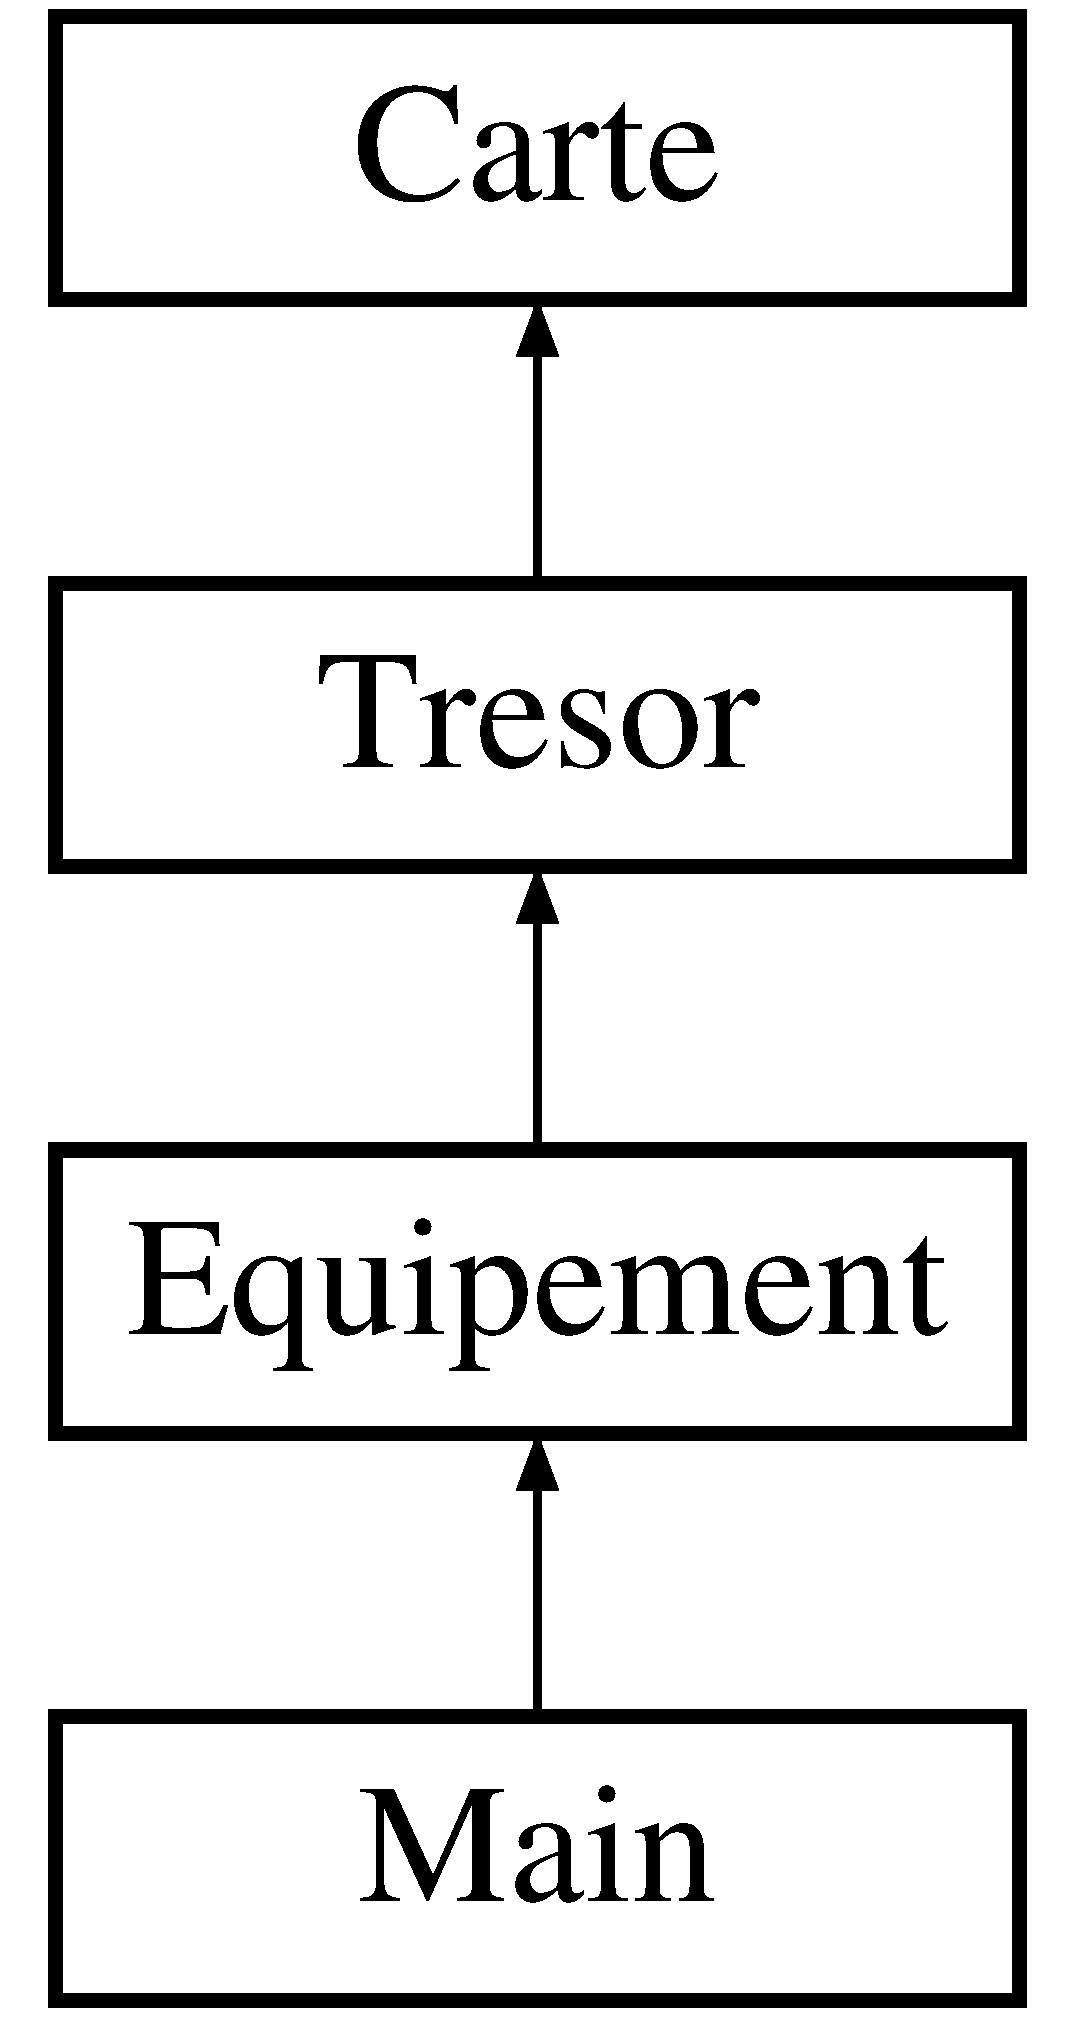
\includegraphics[height=4.000000cm]{class_main}
\end{center}
\end{figure}
\subsection*{Public Member Functions}
\begin{DoxyCompactItemize}
\item 
\hypertarget{class_main_ad94c74f168aee209875192dbc37bec24}{{\bfseries Main} (int id, std\-::string n, std\-::string d, int p)}\label{class_main_ad94c74f168aee209875192dbc37bec24}

\item 
\hypertarget{class_main_aeb10b51d05314910f7d264c438835216}{{\bfseries Main} (int id, std\-::string n, std\-::string d, int p, int nb)}\label{class_main_aeb10b51d05314910f7d264c438835216}

\item 
int \hyperlink{class_main_a2a7c731f2f24128a76a80bb7a0ea1a9a}{get\-Nb\-Main} ()
\begin{DoxyCompactList}\small\item\em Renvoie le nombre de mains prises par l'objet. \end{DoxyCompactList}\item 
bool \hyperlink{class_main_aba193ef84e793b04254c1a13031a0c92}{est\-Main} ()
\begin{DoxyCompactList}\small\item\em Renvoie vrai si c'est une \hyperlink{class_main}{Main}. \end{DoxyCompactList}\end{DoxyCompactItemize}
\subsection*{Additional Inherited Members}


\subsection{Member Function Documentation}
\hypertarget{class_main_aba193ef84e793b04254c1a13031a0c92}{\index{Main@{Main}!est\-Main@{est\-Main}}
\index{est\-Main@{est\-Main}!Main@{Main}}
\subsubsection[{est\-Main}]{\setlength{\rightskip}{0pt plus 5cm}bool Main\-::est\-Main (
\begin{DoxyParamCaption}
{}
\end{DoxyParamCaption}
)\hspace{0.3cm}{\ttfamily [virtual]}}}\label{class_main_aba193ef84e793b04254c1a13031a0c92}


Renvoie vrai si c'est une \hyperlink{class_main}{Main}. 

\begin{DoxyReturn}{Returns}
vrai si c'est une \hyperlink{class_main}{Main}, Faux sinon 
\end{DoxyReturn}


Reimplemented from \hyperlink{class_carte_a13cfbbcd63cd11659ada554db42f6a3f}{Carte}.

\hypertarget{class_main_a2a7c731f2f24128a76a80bb7a0ea1a9a}{\index{Main@{Main}!get\-Nb\-Main@{get\-Nb\-Main}}
\index{get\-Nb\-Main@{get\-Nb\-Main}!Main@{Main}}
\subsubsection[{get\-Nb\-Main}]{\setlength{\rightskip}{0pt plus 5cm}int Main\-::get\-Nb\-Main (
\begin{DoxyParamCaption}
{}
\end{DoxyParamCaption}
)}}\label{class_main_a2a7c731f2f24128a76a80bb7a0ea1a9a}


Renvoie le nombre de mains prises par l'objet. 

\begin{DoxyReturn}{Returns}
nombre de mains prises par l'objet 
\end{DoxyReturn}


The documentation for this class was generated from the following files\-:\begin{DoxyCompactItemize}
\item 
\hyperlink{_main_8hpp}{Main.\-hpp}\item 
Main.\-cpp\end{DoxyCompactItemize}

\hypertarget{class_malediction}{\section{Malediction Class Reference}
\label{class_malediction}\index{Malediction@{Malediction}}
}
Inheritance diagram for Malediction\-:\begin{figure}[H]
\begin{center}
\leavevmode
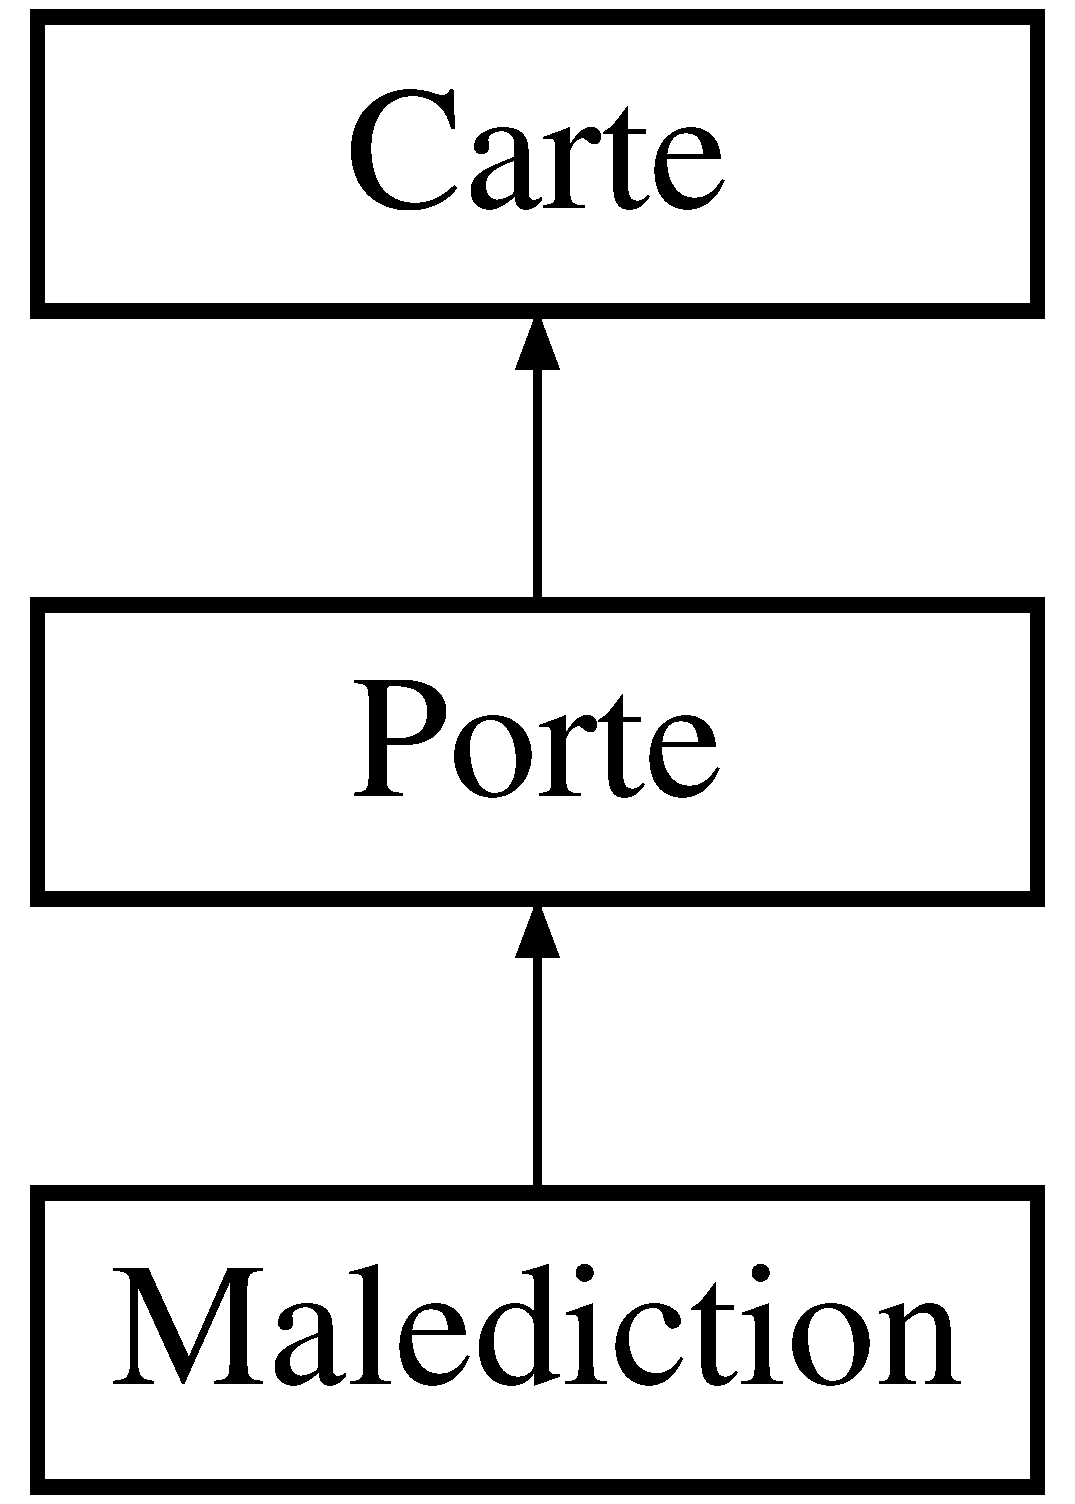
\includegraphics[height=3.000000cm]{class_malediction}
\end{center}
\end{figure}
\subsection*{Public Member Functions}
\begin{DoxyCompactItemize}
\item 
\hypertarget{class_malediction_ac6adc045658a9ec65484bc29940fd3f0}{{\bfseries Malediction} (int id, std\-::string \hyperlink{class_carte_a46bff2b84b76b6b94b2eaa3fe813ec69}{nom}, std\-::string \hyperlink{class_carte_a5f2acc07fa281fb6d4467c00bd4b1614}{description})}\label{class_malediction_ac6adc045658a9ec65484bc29940fd3f0}

\item 
virtual bool \hyperlink{class_malediction_a3e374642e5326239e9d613bd2233c1be}{est\-Malediction} ()
\begin{DoxyCompactList}\small\item\em Renvoie vrai si c'est une \hyperlink{class_malediction}{Malediction}. \end{DoxyCompactList}\end{DoxyCompactItemize}
\subsection*{Additional Inherited Members}


\subsection{Member Function Documentation}
\hypertarget{class_malediction_a3e374642e5326239e9d613bd2233c1be}{\index{Malediction@{Malediction}!est\-Malediction@{est\-Malediction}}
\index{est\-Malediction@{est\-Malediction}!Malediction@{Malediction}}
\subsubsection[{est\-Malediction}]{\setlength{\rightskip}{0pt plus 5cm}bool Malediction\-::est\-Malediction (
\begin{DoxyParamCaption}
{}
\end{DoxyParamCaption}
)\hspace{0.3cm}{\ttfamily [virtual]}}}\label{class_malediction_a3e374642e5326239e9d613bd2233c1be}


Renvoie vrai si c'est une \hyperlink{class_malediction}{Malediction}. 

\begin{DoxyReturn}{Returns}
vrai si c'est une \hyperlink{class_malediction}{Malediction}, Faux sinon 
\end{DoxyReturn}


Reimplemented from \hyperlink{class_carte_af9c84ec45b9a570d8ac8019726756ee7}{Carte}.



The documentation for this class was generated from the following files\-:\begin{DoxyCompactItemize}
\item 
\hyperlink{_malediction_8hpp}{Malediction.\-hpp}\item 
\hyperlink{_malediction_8cpp}{Malediction.\-cpp}\end{DoxyCompactItemize}

\hypertarget{class_malus_bonus}{\section{Malus\-Bonus Class Reference}
\label{class_malus_bonus}\index{Malus\-Bonus@{Malus\-Bonus}}
}
Inheritance diagram for Malus\-Bonus\-:\begin{figure}[H]
\begin{center}
\leavevmode
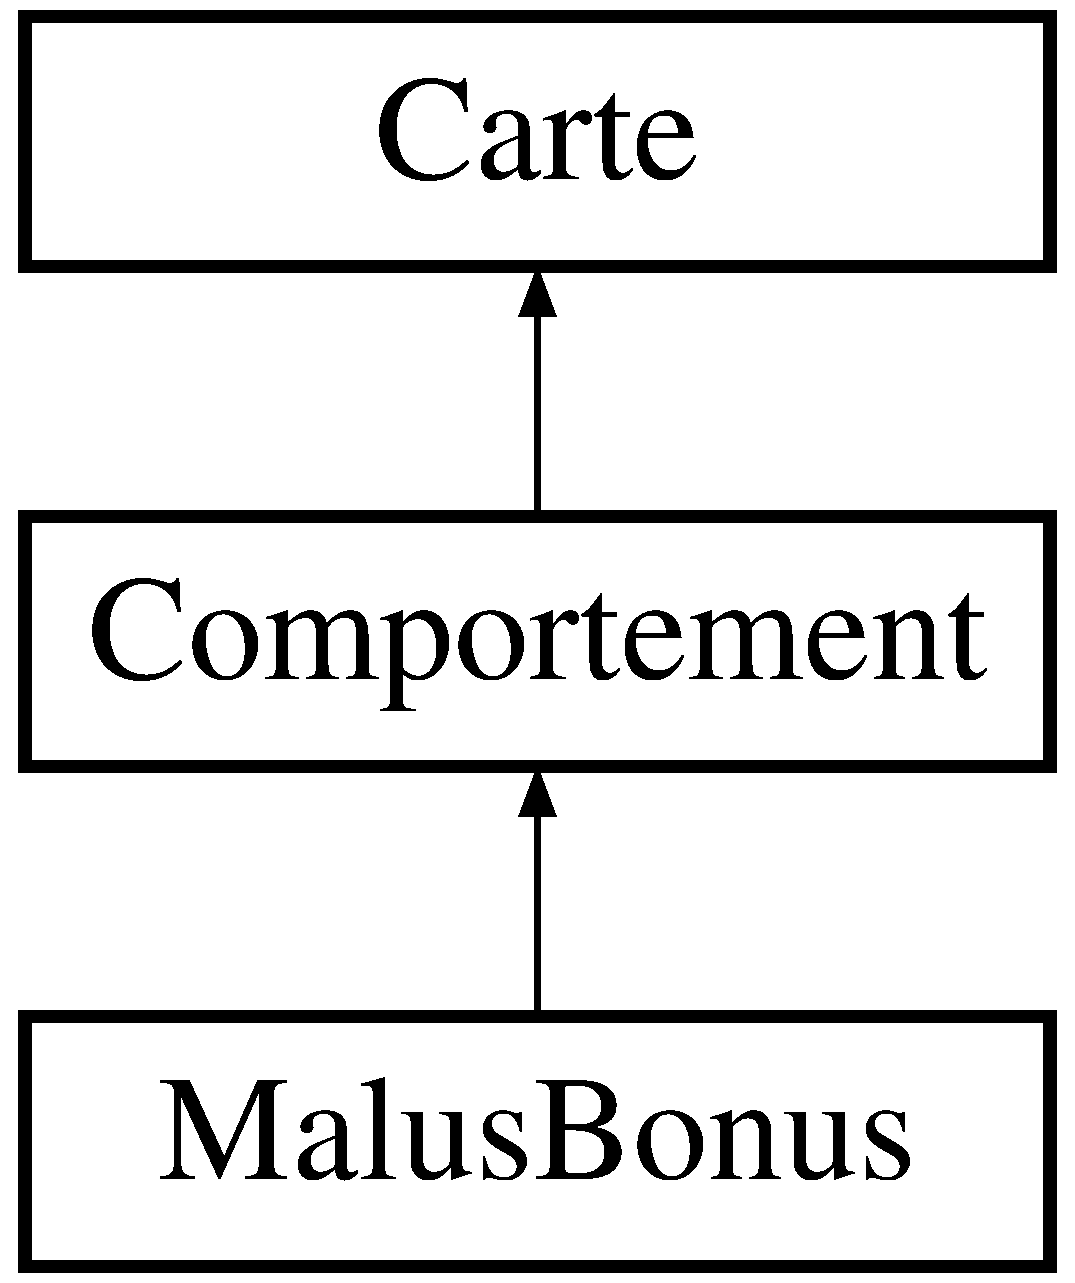
\includegraphics[height=3.000000cm]{class_malus_bonus}
\end{center}
\end{figure}
\subsection*{Public Member Functions}
\begin{DoxyCompactItemize}
\item 
\hyperlink{class_malus_bonus_a730f17b06282de4d63ba3cd078cce92f}{Malus\-Bonus} (\hyperlink{class_carte}{Carte} $\ast$c, int v)
\begin{DoxyCompactList}\small\item\em Constructeur de \hyperlink{class_malus_bonus}{Malus\-Bonus}. \end{DoxyCompactList}\item 
\hypertarget{class_malus_bonus_a83acf04a0977f8e4703d675bd1d68c56}{\hyperlink{class_malus_bonus_a83acf04a0977f8e4703d675bd1d68c56}{$\sim$\-Malus\-Bonus} ()}\label{class_malus_bonus_a83acf04a0977f8e4703d675bd1d68c56}

\begin{DoxyCompactList}\small\item\em Destructeur de \hyperlink{class_malus_bonus}{Malus\-Bonus}. \end{DoxyCompactList}\item 
virtual void \hyperlink{class_malus_bonus_aede2c45aa2a0d0f751c128e05d26fb6a}{appliquer} (\hyperlink{class_personnage}{Personnage} $\ast$p)
\begin{DoxyCompactList}\small\item\em applique le comportement de la carte \end{DoxyCompactList}\item 
virtual void \hyperlink{class_malus_bonus_a213a8e9301ac84e2cf338476bf6613fc}{retirer} (\hyperlink{class_personnage}{Personnage} $\ast$p)
\begin{DoxyCompactList}\small\item\em retire le comportement de la carte \end{DoxyCompactList}\end{DoxyCompactItemize}
\subsection*{Additional Inherited Members}


\subsection{Constructor \& Destructor Documentation}
\hypertarget{class_malus_bonus_a730f17b06282de4d63ba3cd078cce92f}{\index{Malus\-Bonus@{Malus\-Bonus}!Malus\-Bonus@{Malus\-Bonus}}
\index{Malus\-Bonus@{Malus\-Bonus}!MalusBonus@{Malus\-Bonus}}
\subsubsection[{Malus\-Bonus}]{\setlength{\rightskip}{0pt plus 5cm}Malus\-Bonus\-::\-Malus\-Bonus (
\begin{DoxyParamCaption}
\item[{{\bf Carte} $\ast$}]{c, }
\item[{int}]{v}
\end{DoxyParamCaption}
)}}\label{class_malus_bonus_a730f17b06282de4d63ba3cd078cce92f}


Constructeur de \hyperlink{class_malus_bonus}{Malus\-Bonus}. 


\begin{DoxyParams}{Parameters}
{\em c} & \hyperlink{class_carte}{Carte} décorée \\
\hline
{\em valeur} & Valeur du comportement \\
\hline
\end{DoxyParams}


\subsection{Member Function Documentation}
\hypertarget{class_malus_bonus_aede2c45aa2a0d0f751c128e05d26fb6a}{\index{Malus\-Bonus@{Malus\-Bonus}!appliquer@{appliquer}}
\index{appliquer@{appliquer}!MalusBonus@{Malus\-Bonus}}
\subsubsection[{appliquer}]{\setlength{\rightskip}{0pt plus 5cm}void Malus\-Bonus\-::appliquer (
\begin{DoxyParamCaption}
\item[{{\bf Personnage} $\ast$}]{p}
\end{DoxyParamCaption}
)\hspace{0.3cm}{\ttfamily [virtual]}}}\label{class_malus_bonus_aede2c45aa2a0d0f751c128e05d26fb6a}


applique le comportement de la carte 


\begin{DoxyParams}{Parameters}
{\em cible} & du comportement \\
\hline
\end{DoxyParams}


Reimplemented from \hyperlink{class_comportement_ae55149d29c710b0a5a0388cae308024f}{Comportement}.

\hypertarget{class_malus_bonus_a213a8e9301ac84e2cf338476bf6613fc}{\index{Malus\-Bonus@{Malus\-Bonus}!retirer@{retirer}}
\index{retirer@{retirer}!MalusBonus@{Malus\-Bonus}}
\subsubsection[{retirer}]{\setlength{\rightskip}{0pt plus 5cm}void Malus\-Bonus\-::retirer (
\begin{DoxyParamCaption}
\item[{{\bf Personnage} $\ast$}]{p}
\end{DoxyParamCaption}
)\hspace{0.3cm}{\ttfamily [virtual]}}}\label{class_malus_bonus_a213a8e9301ac84e2cf338476bf6613fc}


retire le comportement de la carte 


\begin{DoxyParams}{Parameters}
{\em cible} & du comportement \\
\hline
\end{DoxyParams}


Reimplemented from \hyperlink{class_comportement_a7be9c46a6ae6d49ca3f49288b438b689}{Comportement}.



The documentation for this class was generated from the following files\-:\begin{DoxyCompactItemize}
\item 
\hyperlink{_malus_bonus_8hpp}{Malus\-Bonus.\-hpp}\item 
\hyperlink{_malus_bonus_8cpp}{Malus\-Bonus.\-cpp}\end{DoxyCompactItemize}

\hypertarget{class_malus_bonus_deguerpir}{\section{Malus\-Bonus\-Deguerpir Class Reference}
\label{class_malus_bonus_deguerpir}\index{Malus\-Bonus\-Deguerpir@{Malus\-Bonus\-Deguerpir}}
}
Inheritance diagram for Malus\-Bonus\-Deguerpir\-:\begin{figure}[H]
\begin{center}
\leavevmode
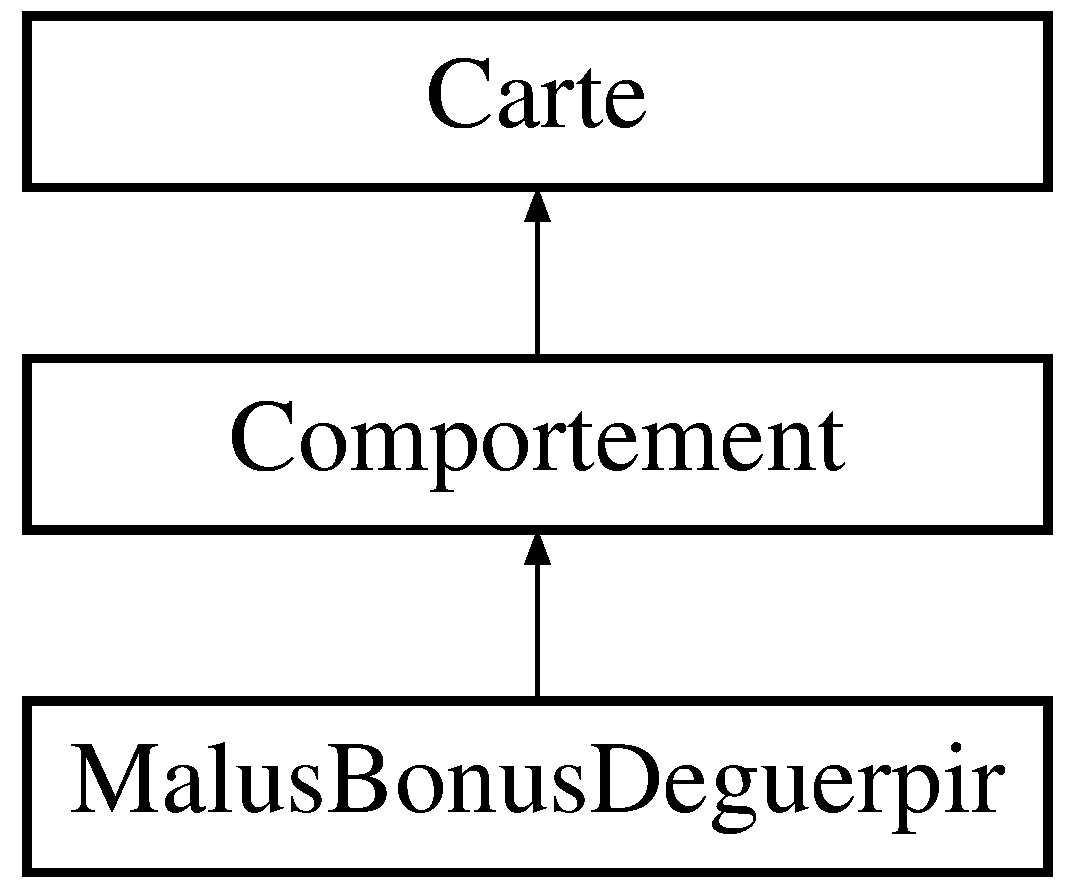
\includegraphics[height=3.000000cm]{class_malus_bonus_deguerpir}
\end{center}
\end{figure}
\subsection*{Public Member Functions}
\begin{DoxyCompactItemize}
\item 
\hyperlink{class_malus_bonus_deguerpir_a4e45b5b1be3f42cd2740294aaca609a0}{Malus\-Bonus\-Deguerpir} (\hyperlink{class_carte}{Carte} $\ast$c, int v)
\begin{DoxyCompactList}\small\item\em Constructeur de \hyperlink{class_malus_bonus_deguerpir}{Malus\-Bonus\-Deguerpir}. \end{DoxyCompactList}\item 
\hypertarget{class_malus_bonus_deguerpir_a9225653a1da567b995bead68d512a3e3}{\hyperlink{class_malus_bonus_deguerpir_a9225653a1da567b995bead68d512a3e3}{$\sim$\-Malus\-Bonus\-Deguerpir} ()}\label{class_malus_bonus_deguerpir_a9225653a1da567b995bead68d512a3e3}

\begin{DoxyCompactList}\small\item\em Destructeur de \hyperlink{class_malus_bonus_deguerpir}{Malus\-Bonus\-Deguerpir}. \end{DoxyCompactList}\item 
virtual void \hyperlink{class_malus_bonus_deguerpir_a703620e87d5d861ba850a3b07f61195a}{appliquer} (\hyperlink{class_personnage}{Personnage} $\ast$p)
\begin{DoxyCompactList}\small\item\em applique le comportement de la carte \end{DoxyCompactList}\item 
virtual void \hyperlink{class_malus_bonus_deguerpir_af7889dc668d138990d4e255c76bb8a89}{retirer} (\hyperlink{class_personnage}{Personnage} $\ast$p)
\begin{DoxyCompactList}\small\item\em retire le comportement de la carte \end{DoxyCompactList}\end{DoxyCompactItemize}
\subsection*{Additional Inherited Members}


\subsection{Constructor \& Destructor Documentation}
\hypertarget{class_malus_bonus_deguerpir_a4e45b5b1be3f42cd2740294aaca609a0}{\index{Malus\-Bonus\-Deguerpir@{Malus\-Bonus\-Deguerpir}!Malus\-Bonus\-Deguerpir@{Malus\-Bonus\-Deguerpir}}
\index{Malus\-Bonus\-Deguerpir@{Malus\-Bonus\-Deguerpir}!MalusBonusDeguerpir@{Malus\-Bonus\-Deguerpir}}
\subsubsection[{Malus\-Bonus\-Deguerpir}]{\setlength{\rightskip}{0pt plus 5cm}Malus\-Bonus\-Deguerpir\-::\-Malus\-Bonus\-Deguerpir (
\begin{DoxyParamCaption}
\item[{{\bf Carte} $\ast$}]{c, }
\item[{int}]{v}
\end{DoxyParamCaption}
)}}\label{class_malus_bonus_deguerpir_a4e45b5b1be3f42cd2740294aaca609a0}


Constructeur de \hyperlink{class_malus_bonus_deguerpir}{Malus\-Bonus\-Deguerpir}. 


\begin{DoxyParams}{Parameters}
{\em c} & \hyperlink{class_carte}{Carte} décorée \\
\hline
{\em valeur} & Valeur du comportement \\
\hline
\end{DoxyParams}


\subsection{Member Function Documentation}
\hypertarget{class_malus_bonus_deguerpir_a703620e87d5d861ba850a3b07f61195a}{\index{Malus\-Bonus\-Deguerpir@{Malus\-Bonus\-Deguerpir}!appliquer@{appliquer}}
\index{appliquer@{appliquer}!MalusBonusDeguerpir@{Malus\-Bonus\-Deguerpir}}
\subsubsection[{appliquer}]{\setlength{\rightskip}{0pt plus 5cm}void Malus\-Bonus\-Deguerpir\-::appliquer (
\begin{DoxyParamCaption}
\item[{{\bf Personnage} $\ast$}]{p}
\end{DoxyParamCaption}
)\hspace{0.3cm}{\ttfamily [virtual]}}}\label{class_malus_bonus_deguerpir_a703620e87d5d861ba850a3b07f61195a}


applique le comportement de la carte 


\begin{DoxyParams}{Parameters}
{\em cible} & du comportement \\
\hline
\end{DoxyParams}


Reimplemented from \hyperlink{class_comportement_ae55149d29c710b0a5a0388cae308024f}{Comportement}.

\hypertarget{class_malus_bonus_deguerpir_af7889dc668d138990d4e255c76bb8a89}{\index{Malus\-Bonus\-Deguerpir@{Malus\-Bonus\-Deguerpir}!retirer@{retirer}}
\index{retirer@{retirer}!MalusBonusDeguerpir@{Malus\-Bonus\-Deguerpir}}
\subsubsection[{retirer}]{\setlength{\rightskip}{0pt plus 5cm}void Malus\-Bonus\-Deguerpir\-::retirer (
\begin{DoxyParamCaption}
\item[{{\bf Personnage} $\ast$}]{p}
\end{DoxyParamCaption}
)\hspace{0.3cm}{\ttfamily [virtual]}}}\label{class_malus_bonus_deguerpir_af7889dc668d138990d4e255c76bb8a89}


retire le comportement de la carte 


\begin{DoxyParams}{Parameters}
{\em cible} & du comportement \\
\hline
\end{DoxyParams}


Reimplemented from \hyperlink{class_comportement_a7be9c46a6ae6d49ca3f49288b438b689}{Comportement}.



The documentation for this class was generated from the following files\-:\begin{DoxyCompactItemize}
\item 
\hyperlink{_malus_bonus_deguerpir_8hpp}{Malus\-Bonus\-Deguerpir.\-hpp}\item 
\hyperlink{_malus_bonus_deguerpir_8cpp}{Malus\-Bonus\-Deguerpir.\-cpp}\end{DoxyCompactItemize}

\hypertarget{class_monstre}{\section{Monstre Class Reference}
\label{class_monstre}\index{Monstre@{Monstre}}
}
Inheritance diagram for Monstre\-:\begin{figure}[H]
\begin{center}
\leavevmode
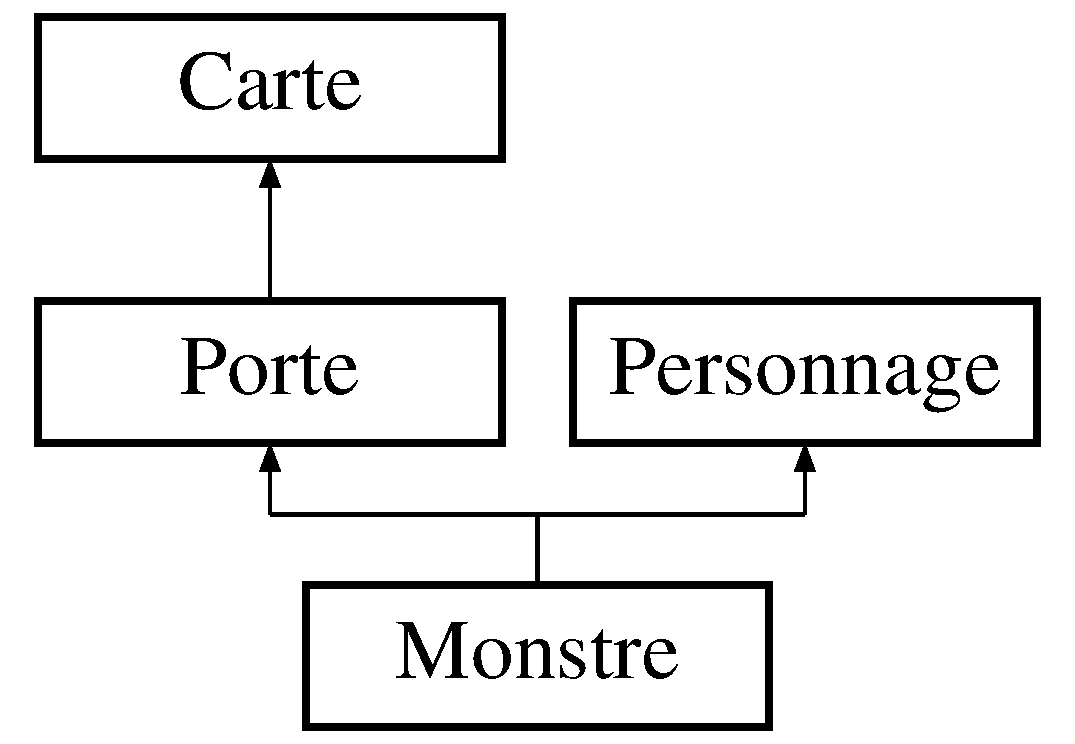
\includegraphics[height=3.000000cm]{class_monstre}
\end{center}
\end{figure}
\subsection*{Public Member Functions}
\begin{DoxyCompactItemize}
\item 
\hyperlink{class_monstre_a9554f4089db262b84c239c54984dbfb3}{Monstre} (int id, std\-::string \hyperlink{class_carte_a46bff2b84b76b6b94b2eaa3fe813ec69}{nom}, std\-::string d, int niv, int nb\-T)
\begin{DoxyCompactList}\small\item\em Constructeur de monstre. \end{DoxyCompactList}\item 
\hypertarget{class_monstre_ac044d27088b58097f6067061807bc708}{{\bfseries Monstre} (int id, std\-::string \hyperlink{class_carte_a46bff2b84b76b6b94b2eaa3fe813ec69}{nom}, std\-::string d, int niv, int nb\-T, int nb\-N)}\label{class_monstre_ac044d27088b58097f6067061807bc708}

\item 
\hypertarget{class_monstre_a8e736b63ae1f561904dad7767448156e}{\hyperlink{class_monstre_a8e736b63ae1f561904dad7767448156e}{$\sim$\-Monstre} ()}\label{class_monstre_a8e736b63ae1f561904dad7767448156e}

\begin{DoxyCompactList}\small\item\em Destructeur de monstre. \end{DoxyCompactList}\item 
int \hyperlink{class_monstre_aa73fc24d772d34a9091f4d36d26470eb}{get\-Tresors} ()
\begin{DoxyCompactList}\small\item\em renvoie le nombre de tr�sors que donne le monstre \end{DoxyCompactList}\item 
int \hyperlink{class_monstre_aa10c23979f1f83bac9814c13e312bae0}{get\-Nb\-Niv} ()
\begin{DoxyCompactList}\small\item\em renvoie le nombre de niveaux que donne le monstre \end{DoxyCompactList}\item 
bool \hyperlink{class_monstre_ad01432b5c676e4607e550d4c5595d5ea}{est\-Monstre} ()
\begin{DoxyCompactList}\small\item\em Renvoie vrai si c'est un \hyperlink{class_monstre}{Monstre}. \end{DoxyCompactList}\end{DoxyCompactItemize}
\subsection*{Additional Inherited Members}


\subsection{Constructor \& Destructor Documentation}
\hypertarget{class_monstre_a9554f4089db262b84c239c54984dbfb3}{\index{Monstre@{Monstre}!Monstre@{Monstre}}
\index{Monstre@{Monstre}!Monstre@{Monstre}}
\subsubsection[{Monstre}]{\setlength{\rightskip}{0pt plus 5cm}Monstre\-::\-Monstre (
\begin{DoxyParamCaption}
\item[{int}]{id, }
\item[{std\-::string}]{nom, }
\item[{std\-::string}]{d, }
\item[{int}]{niv, }
\item[{int}]{nb\-T}
\end{DoxyParamCaption}
)}}\label{class_monstre_a9554f4089db262b84c239c54984dbfb3}


Constructeur de monstre. 


\begin{DoxyParams}{Parameters}
{\em id} & Identifiant de la carte \\
\hline
{\em nom} & nom de la carte \\
\hline
{\em d} & description de la carte \\
\hline
{\em niv} & niveau du monstre \\
\hline
{\em nb\-T} & nombre de tr�sor que donne le monstre\\
\hline
{\em id} & Identifiant de la carte \\
\hline
{\em nom} & nom de la carte \\
\hline
{\em d} & description de la carte \\
\hline
{\em niv} & niveau du monstre \\
\hline
{\em nb\-T} & nombre de tr�sors que donne le monstre \\
\hline
{\em nb\-N} & nombre de niveaux que donne le monstre \\
\hline
\end{DoxyParams}


\subsection{Member Function Documentation}
\hypertarget{class_monstre_ad01432b5c676e4607e550d4c5595d5ea}{\index{Monstre@{Monstre}!est\-Monstre@{est\-Monstre}}
\index{est\-Monstre@{est\-Monstre}!Monstre@{Monstre}}
\subsubsection[{est\-Monstre}]{\setlength{\rightskip}{0pt plus 5cm}bool Monstre\-::est\-Monstre (
\begin{DoxyParamCaption}
{}
\end{DoxyParamCaption}
)\hspace{0.3cm}{\ttfamily [virtual]}}}\label{class_monstre_ad01432b5c676e4607e550d4c5595d5ea}


Renvoie vrai si c'est un \hyperlink{class_monstre}{Monstre}. 

\begin{DoxyReturn}{Returns}
vrai si c'est un \hyperlink{class_monstre}{Monstre}, Faux sinon 
\end{DoxyReturn}


Reimplemented from \hyperlink{class_carte_a74c9bf2967ea099015d1b96003f9da18}{Carte}.

\hypertarget{class_monstre_aa10c23979f1f83bac9814c13e312bae0}{\index{Monstre@{Monstre}!get\-Nb\-Niv@{get\-Nb\-Niv}}
\index{get\-Nb\-Niv@{get\-Nb\-Niv}!Monstre@{Monstre}}
\subsubsection[{get\-Nb\-Niv}]{\setlength{\rightskip}{0pt plus 5cm}int Monstre\-::get\-Nb\-Niv (
\begin{DoxyParamCaption}
{}
\end{DoxyParamCaption}
)}}\label{class_monstre_aa10c23979f1f83bac9814c13e312bae0}


renvoie le nombre de niveaux que donne le monstre 

\begin{DoxyReturn}{Returns}
nombre de niveaux que donne le monstre 
\end{DoxyReturn}
\hypertarget{class_monstre_aa73fc24d772d34a9091f4d36d26470eb}{\index{Monstre@{Monstre}!get\-Tresors@{get\-Tresors}}
\index{get\-Tresors@{get\-Tresors}!Monstre@{Monstre}}
\subsubsection[{get\-Tresors}]{\setlength{\rightskip}{0pt plus 5cm}int Monstre\-::get\-Tresors (
\begin{DoxyParamCaption}
{}
\end{DoxyParamCaption}
)}}\label{class_monstre_aa73fc24d772d34a9091f4d36d26470eb}


renvoie le nombre de tr�sors que donne le monstre 

\begin{DoxyReturn}{Returns}
nombre de tr�sors que donne le monstre 
\end{DoxyReturn}


The documentation for this class was generated from the following files\-:\begin{DoxyCompactItemize}
\item 
\hyperlink{_monstre_8hpp}{Monstre.\-hpp}\item 
\hyperlink{_monstre_8cpp}{Monstre.\-cpp}\end{DoxyCompactItemize}

\hypertarget{class_munchkin}{\section{Munchkin Class Reference}
\label{class_munchkin}\index{Munchkin@{Munchkin}}
}
\subsection*{Public Member Functions}
\begin{DoxyCompactItemize}
\item 
\hyperlink{class_munchkin_a7405ce09c2fecf6a7c8aad66b540fe6f}{Munchkin} (std\-::string filename, int nb\-Joueurs)
\begin{DoxyCompactList}\small\item\em Constructeur. \end{DoxyCompactList}\item 
\hyperlink{class_munchkin_afeca2de58c0d97d3c7e8f16cba24f0a9}{$\sim$\-Munchkin} ()
\begin{DoxyCompactList}\small\item\em Destructeur. \end{DoxyCompactList}\item 
std\-::vector$<$ \hyperlink{class_carte}{Carte} $\ast$ $>$ \& \hyperlink{class_munchkin_a9d50d44d8e4c21b7a32e331823cce92a}{get\-Portes} ()
\begin{DoxyCompactList}\small\item\em Retourne la pioche Portes. \end{DoxyCompactList}\item 
std\-::vector$<$ \hyperlink{class_carte}{Carte} $\ast$ $>$ \& \hyperlink{class_munchkin_a6ce31edc0ecf47b7d622842bf3fc4373}{get\-Defausse} ()
\begin{DoxyCompactList}\small\item\em Retourne la defausse. \end{DoxyCompactList}\item 
std\-::vector$<$ \hyperlink{class_carte}{Carte} $\ast$ $>$ \& \hyperlink{class_munchkin_a4a28077ee688d85c6c4191f46f4edd4e}{get\-Tresors} ()
\begin{DoxyCompactList}\small\item\em Retourne la pioche Tresors. \end{DoxyCompactList}\item 
std\-::vector$<$ \hyperlink{class_joueur}{Joueur} $\ast$ $>$ \& \hyperlink{class_munchkin_aa6269652a6d729b8fa1df8ab7fa4669f}{get\-Joueurs} ()
\begin{DoxyCompactList}\small\item\em Retourne la liste des joueurs. \end{DoxyCompactList}\item 
\hyperlink{class_joueur}{Joueur} $\ast$ \hyperlink{class_munchkin_a8f8eca21f40abd8b0bb975de1890ac2c}{get\-Courant} ()
\begin{DoxyCompactList}\small\item\em Retourne le joueur en cours d'action. \end{DoxyCompactList}\item 
bool \hyperlink{class_munchkin_aa6dda31114e2944e25db91abc70c621b}{get\-Fin\-Partie} ()
\begin{DoxyCompactList}\small\item\em Retourne le bool�en fin\-Partie. \end{DoxyCompactList}\item 
void \hyperlink{class_munchkin_afc5cf1814a138cc62a21721f898d5247}{set\-Fin\-Partie} (bool b)
\begin{DoxyCompactList}\small\item\em Change la valeur de fin\-Partie. \end{DoxyCompactList}\item 
void \hyperlink{class_munchkin_a67a1f016d1722fdb01809448886747a7}{changement\-Joueur} (\hyperlink{class_joueur}{Joueur} $\ast$j)
\begin{DoxyCompactList}\small\item\em Permet de changer la valeur de courant. \end{DoxyCompactList}\item 
void \hyperlink{class_munchkin_a4250c37d0904be46d696ae75be8ca9a2}{importer\-Cartes} (std\-::string filename)
\begin{DoxyCompactList}\small\item\em Importe les cartes d'un fichier texte. \end{DoxyCompactList}\item 
\hyperlink{class_carte}{Carte} $\ast$ \hyperlink{class_munchkin_aa242a4b775ac07b8d135d6c2bcbeb6bb}{piocher\-Porte} ()
\begin{DoxyCompactList}\small\item\em Pioche une porte. \end{DoxyCompactList}\item 
\hyperlink{class_carte}{Carte} $\ast$ \hyperlink{class_munchkin_afdcf1d357b23047721f69c0362edb409}{piocher\-Tresor} ()
\begin{DoxyCompactList}\small\item\em Pioche un tresor. \end{DoxyCompactList}\item 
void \hyperlink{class_munchkin_aaba52b8ae44b3dd067a5805a7614c942}{defausser} (\hyperlink{class_carte}{Carte} $\ast$c)
\begin{DoxyCompactList}\small\item\em Defausse une carte. \end{DoxyCompactList}\end{DoxyCompactItemize}


\subsection{Constructor \& Destructor Documentation}
\hypertarget{class_munchkin_a7405ce09c2fecf6a7c8aad66b540fe6f}{\index{Munchkin@{Munchkin}!Munchkin@{Munchkin}}
\index{Munchkin@{Munchkin}!Munchkin@{Munchkin}}
\subsubsection[{Munchkin}]{\setlength{\rightskip}{0pt plus 5cm}Munchkin\-::\-Munchkin (
\begin{DoxyParamCaption}
\item[{std\-::string}]{filename, }
\item[{int}]{nb\-Joueurs}
\end{DoxyParamCaption}
)}}\label{class_munchkin_a7405ce09c2fecf6a7c8aad66b540fe6f}


Constructeur. 

Constructeur de la classe \hyperlink{class_munchkin}{Munchkin}.


\begin{DoxyParams}{Parameters}
{\em filename} & \-: Chemin d'Acc�s au documents contenant les cartes. \\
\hline
{\em nb\-Joueurs} & \-: Nombre de joueurs dans la partie. \\
\hline
\end{DoxyParams}
\hypertarget{class_munchkin_afeca2de58c0d97d3c7e8f16cba24f0a9}{\index{Munchkin@{Munchkin}!$\sim$\-Munchkin@{$\sim$\-Munchkin}}
\index{$\sim$\-Munchkin@{$\sim$\-Munchkin}!Munchkin@{Munchkin}}
\subsubsection[{$\sim$\-Munchkin}]{\setlength{\rightskip}{0pt plus 5cm}Munchkin\-::$\sim$\-Munchkin (
\begin{DoxyParamCaption}
{}
\end{DoxyParamCaption}
)}}\label{class_munchkin_afeca2de58c0d97d3c7e8f16cba24f0a9}


Destructeur. 

Destructeur de la classe \hyperlink{class_munchkin}{Munchkin}. 

\subsection{Member Function Documentation}
\hypertarget{class_munchkin_a67a1f016d1722fdb01809448886747a7}{\index{Munchkin@{Munchkin}!changement\-Joueur@{changement\-Joueur}}
\index{changement\-Joueur@{changement\-Joueur}!Munchkin@{Munchkin}}
\subsubsection[{changement\-Joueur}]{\setlength{\rightskip}{0pt plus 5cm}void Munchkin\-::changement\-Joueur (
\begin{DoxyParamCaption}
\item[{{\bf Joueur} $\ast$}]{j}
\end{DoxyParamCaption}
)}}\label{class_munchkin_a67a1f016d1722fdb01809448886747a7}


Permet de changer la valeur de courant. 

Methode qui de modifier le \hyperlink{class_joueur}{Joueur} dont il c'est actuelement le tour


\begin{DoxyParams}{Parameters}
{\em j} & \-: Nouveau joueur en cour d'action. \\
\hline
\end{DoxyParams}
\hypertarget{class_munchkin_aaba52b8ae44b3dd067a5805a7614c942}{\index{Munchkin@{Munchkin}!defausser@{defausser}}
\index{defausser@{defausser}!Munchkin@{Munchkin}}
\subsubsection[{defausser}]{\setlength{\rightskip}{0pt plus 5cm}void Munchkin\-::defausser (
\begin{DoxyParamCaption}
\item[{{\bf Carte} $\ast$}]{c}
\end{DoxyParamCaption}
)}}\label{class_munchkin_aaba52b8ae44b3dd067a5805a7614c942}


Defausse une carte. 

M�thode qui ajoute la carte pass� en parametre a la liste defausse.


\begin{DoxyParams}{Parameters}
{\em c} & \-: \hyperlink{class_carte}{Carte} a ajouter a la d�fausse. \\
\hline
\end{DoxyParams}
\hypertarget{class_munchkin_a8f8eca21f40abd8b0bb975de1890ac2c}{\index{Munchkin@{Munchkin}!get\-Courant@{get\-Courant}}
\index{get\-Courant@{get\-Courant}!Munchkin@{Munchkin}}
\subsubsection[{get\-Courant}]{\setlength{\rightskip}{0pt plus 5cm}{\bf Joueur} $\ast$ Munchkin\-::get\-Courant (
\begin{DoxyParamCaption}
{}
\end{DoxyParamCaption}
)}}\label{class_munchkin_a8f8eca21f40abd8b0bb975de1890ac2c}


Retourne le joueur en cours d'action. 

Methode qui retoune le joueur qui est acctuelement en train d'effectuer son tour

\begin{DoxyReturn}{Returns}
un \hyperlink{class_joueur}{Joueur} 
\end{DoxyReturn}
\hypertarget{class_munchkin_a6ce31edc0ecf47b7d622842bf3fc4373}{\index{Munchkin@{Munchkin}!get\-Defausse@{get\-Defausse}}
\index{get\-Defausse@{get\-Defausse}!Munchkin@{Munchkin}}
\subsubsection[{get\-Defausse}]{\setlength{\rightskip}{0pt plus 5cm}std\-::vector$<$ {\bf Carte} $\ast$ $>$ \& Munchkin\-::get\-Defausse (
\begin{DoxyParamCaption}
{}
\end{DoxyParamCaption}
)}}\label{class_munchkin_a6ce31edc0ecf47b7d622842bf3fc4373}


Retourne la defausse. 

Retourne la liste des cartes de la defausse

\begin{DoxyReturn}{Returns}
une liste de \hyperlink{class_carte}{Carte} 
\end{DoxyReturn}
\hypertarget{class_munchkin_aa6dda31114e2944e25db91abc70c621b}{\index{Munchkin@{Munchkin}!get\-Fin\-Partie@{get\-Fin\-Partie}}
\index{get\-Fin\-Partie@{get\-Fin\-Partie}!Munchkin@{Munchkin}}
\subsubsection[{get\-Fin\-Partie}]{\setlength{\rightskip}{0pt plus 5cm}bool Munchkin\-::get\-Fin\-Partie (
\begin{DoxyParamCaption}
{}
\end{DoxyParamCaption}
)}}\label{class_munchkin_aa6dda31114e2944e25db91abc70c621b}


Retourne le bool�en fin\-Partie. 

Methode qui permet de savoir si le jeu est fini ou toujours en cours.

\begin{DoxyReturn}{Returns}
Retourne un bool�en. 
\end{DoxyReturn}
\hypertarget{class_munchkin_aa6269652a6d729b8fa1df8ab7fa4669f}{\index{Munchkin@{Munchkin}!get\-Joueurs@{get\-Joueurs}}
\index{get\-Joueurs@{get\-Joueurs}!Munchkin@{Munchkin}}
\subsubsection[{get\-Joueurs}]{\setlength{\rightskip}{0pt plus 5cm}std\-::vector$<$ {\bf Joueur} $\ast$ $>$ \& Munchkin\-::get\-Joueurs (
\begin{DoxyParamCaption}
{}
\end{DoxyParamCaption}
)}}\label{class_munchkin_aa6269652a6d729b8fa1df8ab7fa4669f}


Retourne la liste des joueurs. 

Methode qui retourne les joueurs du munchkin

\begin{DoxyReturn}{Returns}
une liste de \hyperlink{class_joueur}{Joueur} 
\end{DoxyReturn}
\hypertarget{class_munchkin_a9d50d44d8e4c21b7a32e331823cce92a}{\index{Munchkin@{Munchkin}!get\-Portes@{get\-Portes}}
\index{get\-Portes@{get\-Portes}!Munchkin@{Munchkin}}
\subsubsection[{get\-Portes}]{\setlength{\rightskip}{0pt plus 5cm}std\-::vector$<$ {\bf Carte} $\ast$ $>$ \& Munchkin\-::get\-Portes (
\begin{DoxyParamCaption}
{}
\end{DoxyParamCaption}
)}}\label{class_munchkin_a9d50d44d8e4c21b7a32e331823cce92a}


Retourne la pioche Portes. 

Retourne la liste des cartes portes de la pioche Portes

\begin{DoxyReturn}{Returns}
une liste de \hyperlink{class_carte}{Carte} 
\end{DoxyReturn}
\hypertarget{class_munchkin_a4a28077ee688d85c6c4191f46f4edd4e}{\index{Munchkin@{Munchkin}!get\-Tresors@{get\-Tresors}}
\index{get\-Tresors@{get\-Tresors}!Munchkin@{Munchkin}}
\subsubsection[{get\-Tresors}]{\setlength{\rightskip}{0pt plus 5cm}std\-::vector$<$ {\bf Carte} $\ast$ $>$ \& Munchkin\-::get\-Tresors (
\begin{DoxyParamCaption}
{}
\end{DoxyParamCaption}
)}}\label{class_munchkin_a4a28077ee688d85c6c4191f46f4edd4e}


Retourne la pioche Tresors. 

Retourne la liste des cartes de la pioche Tresors

\begin{DoxyReturn}{Returns}
une liste de \hyperlink{class_carte}{Carte} 
\end{DoxyReturn}
\hypertarget{class_munchkin_a4250c37d0904be46d696ae75be8ca9a2}{\index{Munchkin@{Munchkin}!importer\-Cartes@{importer\-Cartes}}
\index{importer\-Cartes@{importer\-Cartes}!Munchkin@{Munchkin}}
\subsubsection[{importer\-Cartes}]{\setlength{\rightskip}{0pt plus 5cm}void Munchkin\-::importer\-Cartes (
\begin{DoxyParamCaption}
\item[{std\-::string}]{filename}
\end{DoxyParamCaption}
)}}\label{class_munchkin_a4250c37d0904be46d696ae75be8ca9a2}


Importe les cartes d'un fichier texte. 

Methode appel les fabrique de carte pour ajouter des cartes au jeu depuis un fichier texte.


\begin{DoxyParams}{Parameters}
{\em filename} & \-: Chemin d'Acc�s au documents contenant les cartes. \\
\hline
\end{DoxyParams}
\hypertarget{class_munchkin_aa242a4b775ac07b8d135d6c2bcbeb6bb}{\index{Munchkin@{Munchkin}!piocher\-Porte@{piocher\-Porte}}
\index{piocher\-Porte@{piocher\-Porte}!Munchkin@{Munchkin}}
\subsubsection[{piocher\-Porte}]{\setlength{\rightskip}{0pt plus 5cm}{\bf Carte} $\ast$ Munchkin\-::piocher\-Porte (
\begin{DoxyParamCaption}
{}
\end{DoxyParamCaption}
)}}\label{class_munchkin_aa242a4b775ac07b8d135d6c2bcbeb6bb}


Pioche une porte. 

Methode qui retourne une carte de la liste de carte \hyperlink{class_porte}{Porte}.

\begin{DoxyReturn}{Returns}
Une \hyperlink{class_carte}{Carte} de la liste Portes. 
\end{DoxyReturn}
\hypertarget{class_munchkin_afdcf1d357b23047721f69c0362edb409}{\index{Munchkin@{Munchkin}!piocher\-Tresor@{piocher\-Tresor}}
\index{piocher\-Tresor@{piocher\-Tresor}!Munchkin@{Munchkin}}
\subsubsection[{piocher\-Tresor}]{\setlength{\rightskip}{0pt plus 5cm}{\bf Carte} $\ast$ Munchkin\-::piocher\-Tresor (
\begin{DoxyParamCaption}
{}
\end{DoxyParamCaption}
)}}\label{class_munchkin_afdcf1d357b23047721f69c0362edb409}


Pioche un tresor. 

Methode qui retourne une carte de la liste de carte \hyperlink{class_tresor}{Tresor}.

\begin{DoxyReturn}{Returns}
Une \hyperlink{class_carte}{Carte} de la liste Tresors. 
\end{DoxyReturn}
\hypertarget{class_munchkin_afc5cf1814a138cc62a21721f898d5247}{\index{Munchkin@{Munchkin}!set\-Fin\-Partie@{set\-Fin\-Partie}}
\index{set\-Fin\-Partie@{set\-Fin\-Partie}!Munchkin@{Munchkin}}
\subsubsection[{set\-Fin\-Partie}]{\setlength{\rightskip}{0pt plus 5cm}void Munchkin\-::set\-Fin\-Partie (
\begin{DoxyParamCaption}
\item[{bool}]{b}
\end{DoxyParamCaption}
)}}\label{class_munchkin_afc5cf1814a138cc62a21721f898d5247}


Change la valeur de fin\-Partie. 

Permet de changer la valeur de fin\-Partie remplac� par celle en parametre.


\begin{DoxyParams}{Parameters}
{\em b} & \-: bool�en. \\
\hline
\end{DoxyParams}


The documentation for this class was generated from the following files\-:\begin{DoxyCompactItemize}
\item 
\hyperlink{_munchkin_8hpp}{Munchkin.\-hpp}\item 
\hyperlink{_munchkin_8cpp}{Munchkin.\-cpp}\end{DoxyCompactItemize}

\hypertarget{class_ouvrir_porte}{\section{Ouvrir\-Porte Class Reference}
\label{class_ouvrir_porte}\index{Ouvrir\-Porte@{Ouvrir\-Porte}}
}
Inheritance diagram for Ouvrir\-Porte\-:\begin{figure}[H]
\begin{center}
\leavevmode
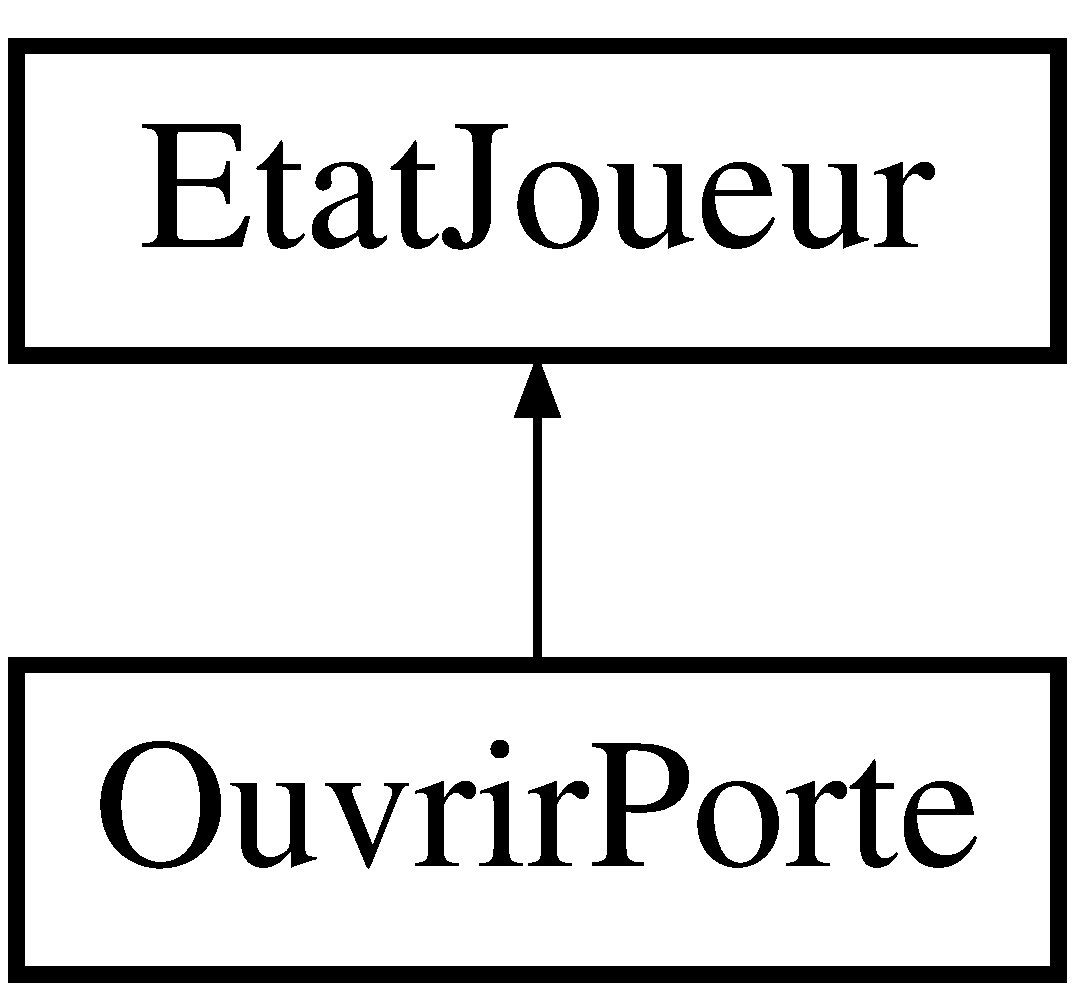
\includegraphics[height=2.000000cm]{class_ouvrir_porte}
\end{center}
\end{figure}
\subsection*{Public Member Functions}
\begin{DoxyCompactItemize}
\item 
\hyperlink{class_ouvrir_porte_a6cd824c78a2293d060721cf8a89bf89b}{Ouvrir\-Porte} (\hyperlink{class_joueur}{Joueur} $\ast$t)
\begin{DoxyCompactList}\small\item\em Constructeur de \hyperlink{class_ouvrir_porte}{Ouvrir\-Porte}. \end{DoxyCompactList}\item 
\hypertarget{class_ouvrir_porte_a001086091ec39ba7c389cdb49c89b722}{virtual \hyperlink{class_ouvrir_porte_a001086091ec39ba7c389cdb49c89b722}{$\sim$\-Ouvrir\-Porte} ()}\label{class_ouvrir_porte_a001086091ec39ba7c389cdb49c89b722}

\begin{DoxyCompactList}\small\item\em Destructeur de \hyperlink{class_ouvrir_porte}{Ouvrir\-Porte}. \end{DoxyCompactList}\item 
\hypertarget{class_ouvrir_porte_aea016cbe6d05c27fcc24bd65565bb657}{void {\bfseries piocher\-Porte\-Face\-Cache} ()}\label{class_ouvrir_porte_aea016cbe6d05c27fcc24bd65565bb657}

\item 
void \hyperlink{class_ouvrir_porte_acd6f890c0ed89e08cb820f547c111591}{changer\-Race} (\hyperlink{class_carte}{Carte} $\ast$r)
\begin{DoxyCompactList}\small\item\em Permet au joueur de changer de race. \end{DoxyCompactList}\item 
void \hyperlink{class_ouvrir_porte_aa674ed243b4fe8575cd9e18b4b1b6990}{pose\-Equipement} (\hyperlink{class_carte}{Carte} $\ast$e)
\begin{DoxyCompactList}\small\item\em Permet au joueur de poser un équipement. \end{DoxyCompactList}\item 
void \hyperlink{class_ouvrir_porte_ad5a18a158f9c677ca24e2f84bc078675}{equiper} (\hyperlink{class_carte}{Carte} $\ast$e)
\begin{DoxyCompactList}\small\item\em Permet au joueur d'équiper un équipement. \end{DoxyCompactList}\item 
void \hyperlink{class_ouvrir_porte_aec4fd339b026b3d122ef0282f48e7a9e}{poser\-Malediction} (\hyperlink{class_joueur}{Joueur} $\ast$cible, \hyperlink{class_carte}{Carte} $\ast$m)
\begin{DoxyCompactList}\small\item\em Permet au joueur de poser une malédiction contre un autre joueur. \end{DoxyCompactList}\item 
void \hyperlink{class_ouvrir_porte_a97795263883803be7189a00756da3ace}{combattre} (\hyperlink{class_carte}{Carte} $\ast$m)
\begin{DoxyCompactList}\small\item\em Permet au joueur de combattre un monstre. \end{DoxyCompactList}\end{DoxyCompactItemize}
\subsection*{Additional Inherited Members}


\subsection{Constructor \& Destructor Documentation}
\hypertarget{class_ouvrir_porte_a6cd824c78a2293d060721cf8a89bf89b}{\index{Ouvrir\-Porte@{Ouvrir\-Porte}!Ouvrir\-Porte@{Ouvrir\-Porte}}
\index{Ouvrir\-Porte@{Ouvrir\-Porte}!OuvrirPorte@{Ouvrir\-Porte}}
\subsubsection[{Ouvrir\-Porte}]{\setlength{\rightskip}{0pt plus 5cm}Ouvrir\-Porte\-::\-Ouvrir\-Porte (
\begin{DoxyParamCaption}
\item[{{\bf Joueur} $\ast$}]{t}
\end{DoxyParamCaption}
)}}\label{class_ouvrir_porte_a6cd824c78a2293d060721cf8a89bf89b}


Constructeur de \hyperlink{class_ouvrir_porte}{Ouvrir\-Porte}. 


\begin{DoxyParams}{Parameters}
{\em t} & \hyperlink{class_joueur}{Joueur} dont l'état doit être géré \\
\hline
\end{DoxyParams}


\subsection{Member Function Documentation}
\hypertarget{class_ouvrir_porte_acd6f890c0ed89e08cb820f547c111591}{\index{Ouvrir\-Porte@{Ouvrir\-Porte}!changer\-Race@{changer\-Race}}
\index{changer\-Race@{changer\-Race}!OuvrirPorte@{Ouvrir\-Porte}}
\subsubsection[{changer\-Race}]{\setlength{\rightskip}{0pt plus 5cm}void Ouvrir\-Porte\-::changer\-Race (
\begin{DoxyParamCaption}
\item[{{\bf Carte} $\ast$}]{r}
\end{DoxyParamCaption}
)\hspace{0.3cm}{\ttfamily [virtual]}}}\label{class_ouvrir_porte_acd6f890c0ed89e08cb820f547c111591}


Permet au joueur de changer de race. 


\begin{DoxyParams}{Parameters}
{\em r} & nouvelle race \\
\hline
\end{DoxyParams}


Reimplemented from \hyperlink{class_etat_joueur_ad60942aa96f0bfb05771f787964887fe}{Etat\-Joueur}.

\hypertarget{class_ouvrir_porte_a97795263883803be7189a00756da3ace}{\index{Ouvrir\-Porte@{Ouvrir\-Porte}!combattre@{combattre}}
\index{combattre@{combattre}!OuvrirPorte@{Ouvrir\-Porte}}
\subsubsection[{combattre}]{\setlength{\rightskip}{0pt plus 5cm}void Ouvrir\-Porte\-::combattre (
\begin{DoxyParamCaption}
\item[{{\bf Carte} $\ast$}]{m}
\end{DoxyParamCaption}
)\hspace{0.3cm}{\ttfamily [virtual]}}}\label{class_ouvrir_porte_a97795263883803be7189a00756da3ace}


Permet au joueur de combattre un monstre. 


\begin{DoxyParams}{Parameters}
{\em m} & monstre à combattre \\
\hline
\end{DoxyParams}


Reimplemented from \hyperlink{class_etat_joueur_a63c672f1d599a82f88aa80aebedf78d6}{Etat\-Joueur}.

\hypertarget{class_ouvrir_porte_ad5a18a158f9c677ca24e2f84bc078675}{\index{Ouvrir\-Porte@{Ouvrir\-Porte}!equiper@{equiper}}
\index{equiper@{equiper}!OuvrirPorte@{Ouvrir\-Porte}}
\subsubsection[{equiper}]{\setlength{\rightskip}{0pt plus 5cm}void Ouvrir\-Porte\-::equiper (
\begin{DoxyParamCaption}
\item[{{\bf Carte} $\ast$}]{e}
\end{DoxyParamCaption}
)\hspace{0.3cm}{\ttfamily [virtual]}}}\label{class_ouvrir_porte_ad5a18a158f9c677ca24e2f84bc078675}


Permet au joueur d'équiper un équipement. 


\begin{DoxyParams}{Parameters}
{\em e} & equipement à équiper \\
\hline
\end{DoxyParams}


Reimplemented from \hyperlink{class_etat_joueur_a2d975d2cd1163a43d6f0002c1f9943e9}{Etat\-Joueur}.

\hypertarget{class_ouvrir_porte_aa674ed243b4fe8575cd9e18b4b1b6990}{\index{Ouvrir\-Porte@{Ouvrir\-Porte}!pose\-Equipement@{pose\-Equipement}}
\index{pose\-Equipement@{pose\-Equipement}!OuvrirPorte@{Ouvrir\-Porte}}
\subsubsection[{pose\-Equipement}]{\setlength{\rightskip}{0pt plus 5cm}void Ouvrir\-Porte\-::pose\-Equipement (
\begin{DoxyParamCaption}
\item[{{\bf Carte} $\ast$}]{e}
\end{DoxyParamCaption}
)\hspace{0.3cm}{\ttfamily [virtual]}}}\label{class_ouvrir_porte_aa674ed243b4fe8575cd9e18b4b1b6990}


Permet au joueur de poser un équipement. 


\begin{DoxyParams}{Parameters}
{\em e} & equipement à poser \\
\hline
\end{DoxyParams}


Reimplemented from \hyperlink{class_etat_joueur_a7d3b72dd7a93a787dcea00d606e9eec2}{Etat\-Joueur}.

\hypertarget{class_ouvrir_porte_aec4fd339b026b3d122ef0282f48e7a9e}{\index{Ouvrir\-Porte@{Ouvrir\-Porte}!poser\-Malediction@{poser\-Malediction}}
\index{poser\-Malediction@{poser\-Malediction}!OuvrirPorte@{Ouvrir\-Porte}}
\subsubsection[{poser\-Malediction}]{\setlength{\rightskip}{0pt plus 5cm}void Ouvrir\-Porte\-::poser\-Malediction (
\begin{DoxyParamCaption}
\item[{{\bf Joueur} $\ast$}]{cible, }
\item[{{\bf Carte} $\ast$}]{m}
\end{DoxyParamCaption}
)\hspace{0.3cm}{\ttfamily [virtual]}}}\label{class_ouvrir_porte_aec4fd339b026b3d122ef0282f48e7a9e}


Permet au joueur de poser une malédiction contre un autre joueur. 


\begin{DoxyParams}{Parameters}
{\em cible} & cible de la malédiction \\
\hline
{\em m} & \hyperlink{class_malediction}{Malediction} à poser \\
\hline
\end{DoxyParams}


Reimplemented from \hyperlink{class_etat_joueur_a6895655263daefa056c3ee11f716cc28}{Etat\-Joueur}.



The documentation for this class was generated from the following files\-:\begin{DoxyCompactItemize}
\item 
\hyperlink{_ouvrir_porte_8hpp}{Ouvrir\-Porte.\-hpp}\item 
\hyperlink{_ouvrir_porte_8cpp}{Ouvrir\-Porte.\-cpp}\end{DoxyCompactItemize}

\hypertarget{class_personnage}{\section{Personnage Class Reference}
\label{class_personnage}\index{Personnage@{Personnage}}
}
Inheritance diagram for Personnage\-:\begin{figure}[H]
\begin{center}
\leavevmode
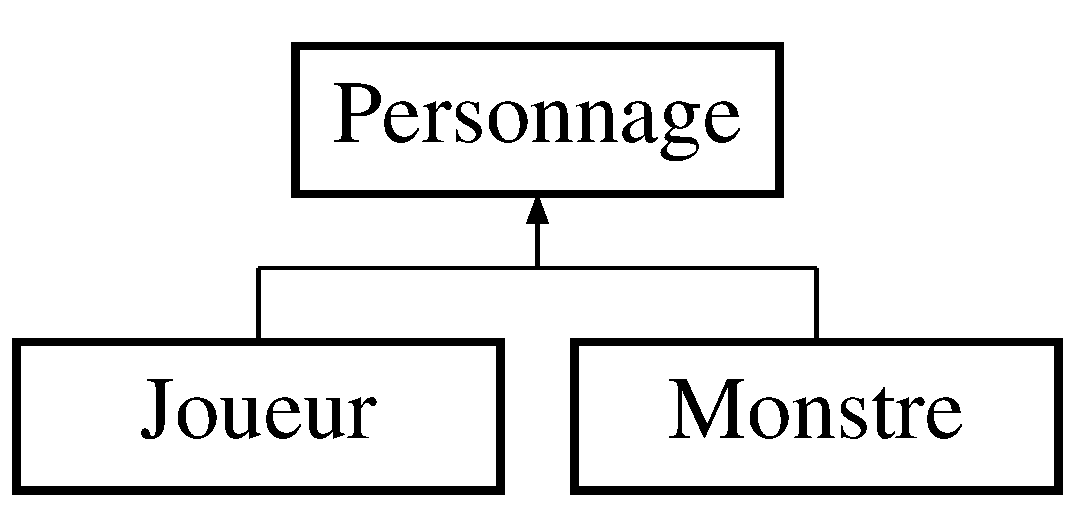
\includegraphics[height=2.000000cm]{class_personnage}
\end{center}
\end{figure}
\subsection*{Public Member Functions}
\begin{DoxyCompactItemize}
\item 
\hyperlink{class_personnage_abec36eb0310adc71f3375297fc590c65}{Personnage} ()
\begin{DoxyCompactList}\small\item\em Constructeur de \hyperlink{class_personnage}{Personnage}. \end{DoxyCompactList}\item 
\hypertarget{class_personnage_ae4757e5ed6f43469b23aa263706bbefc}{{\bfseries Personnage} (int niv)}\label{class_personnage_ae4757e5ed6f43469b23aa263706bbefc}

\item 
\hypertarget{class_personnage_a05bdf2a469885bb1fbb6c2e8f98972ab}{virtual \hyperlink{class_personnage_a05bdf2a469885bb1fbb6c2e8f98972ab}{$\sim$\-Personnage} ()}\label{class_personnage_a05bdf2a469885bb1fbb6c2e8f98972ab}

\begin{DoxyCompactList}\small\item\em Destructeur de \hyperlink{class_personnage}{Personnage}. \end{DoxyCompactList}\item 
int \hyperlink{class_personnage_ac6e8c02d56b789a7c651a551086e1949}{get\-Niveau} ()
\begin{DoxyCompactList}\small\item\em Renvoie le niveau du personnage. \end{DoxyCompactList}\item 
void \hyperlink{class_personnage_aeb57be45e95a868342b16fb27d65367d}{set\-Niveau} (int n)
\begin{DoxyCompactList}\small\item\em Change la valeur du niveau du personnage. \end{DoxyCompactList}\item 
int \hyperlink{class_personnage_a179c739cea6699af03c3e32ba9cf2607}{get\-Bonus} ()
\begin{DoxyCompactList}\small\item\em Renvoie le bonus du personnage. \end{DoxyCompactList}\item 
void \hyperlink{class_personnage_a9f10e5bc14a9fcf2214b4cab0132ea4d}{set\-Bonus} (int b)
\begin{DoxyCompactList}\small\item\em Change la valeur du bonus du personnage. \end{DoxyCompactList}\item 
int \hyperlink{class_personnage_a40de0ba95f25eb6f1653b6a4183763ae}{get\-Force} ()
\begin{DoxyCompactList}\small\item\em Renvoie la force du personnage (bonus+niveau) \end{DoxyCompactList}\item 
void \hyperlink{class_personnage_a2792c711c0ff89db05a83330ffc44d07}{set\-Potion} (\hyperlink{class_carte}{Carte} $\ast$po)
\begin{DoxyCompactList}\small\item\em Ajoute une potion � la liste de potions. \end{DoxyCompactList}\item 
\hypertarget{class_personnage_ac6c7bb3c086c88014c141497ade05c3a}{void \hyperlink{class_personnage_ac6c7bb3c086c88014c141497ade05c3a}{reset\-Potion} ()}\label{class_personnage_ac6c7bb3c086c88014c141497ade05c3a}

\begin{DoxyCompactList}\small\item\em Vide la liste de potions. \end{DoxyCompactList}\end{DoxyCompactItemize}
\subsection*{Protected Attributes}
\begin{DoxyCompactItemize}
\item 
int \hyperlink{class_personnage_a7b310ef7a9567a19724a078172349d89}{niveau}
\item 
int \hyperlink{class_personnage_af212a125f3323df5074dbea5d68ce434}{bonus}
\item 
std\-::vector$<$ \hyperlink{class_carte}{Carte} $\ast$ $>$ \hyperlink{class_personnage_a67b256bffb00b9a097e7b5931113b849}{potions}
\end{DoxyCompactItemize}


\subsection{Constructor \& Destructor Documentation}
\hypertarget{class_personnage_abec36eb0310adc71f3375297fc590c65}{\index{Personnage@{Personnage}!Personnage@{Personnage}}
\index{Personnage@{Personnage}!Personnage@{Personnage}}
\subsubsection[{Personnage}]{\setlength{\rightskip}{0pt plus 5cm}Personnage\-::\-Personnage (
\begin{DoxyParamCaption}
{}
\end{DoxyParamCaption}
)}}\label{class_personnage_abec36eb0310adc71f3375297fc590c65}


Constructeur de \hyperlink{class_personnage}{Personnage}. 


\begin{DoxyParams}{Parameters}
{\em niv} & Niveau du personnage \\
\hline
\end{DoxyParams}


\subsection{Member Function Documentation}
\hypertarget{class_personnage_a179c739cea6699af03c3e32ba9cf2607}{\index{Personnage@{Personnage}!get\-Bonus@{get\-Bonus}}
\index{get\-Bonus@{get\-Bonus}!Personnage@{Personnage}}
\subsubsection[{get\-Bonus}]{\setlength{\rightskip}{0pt plus 5cm}int Personnage\-::get\-Bonus (
\begin{DoxyParamCaption}
{}
\end{DoxyParamCaption}
)}}\label{class_personnage_a179c739cea6699af03c3e32ba9cf2607}


Renvoie le bonus du personnage. 

\begin{DoxyReturn}{Returns}
bonus du personnage 
\end{DoxyReturn}
\hypertarget{class_personnage_a40de0ba95f25eb6f1653b6a4183763ae}{\index{Personnage@{Personnage}!get\-Force@{get\-Force}}
\index{get\-Force@{get\-Force}!Personnage@{Personnage}}
\subsubsection[{get\-Force}]{\setlength{\rightskip}{0pt plus 5cm}int Personnage\-::get\-Force (
\begin{DoxyParamCaption}
{}
\end{DoxyParamCaption}
)}}\label{class_personnage_a40de0ba95f25eb6f1653b6a4183763ae}


Renvoie la force du personnage (bonus+niveau) 

\begin{DoxyReturn}{Returns}
force du personnage 
\end{DoxyReturn}
\hypertarget{class_personnage_ac6e8c02d56b789a7c651a551086e1949}{\index{Personnage@{Personnage}!get\-Niveau@{get\-Niveau}}
\index{get\-Niveau@{get\-Niveau}!Personnage@{Personnage}}
\subsubsection[{get\-Niveau}]{\setlength{\rightskip}{0pt plus 5cm}int Personnage\-::get\-Niveau (
\begin{DoxyParamCaption}
{}
\end{DoxyParamCaption}
)}}\label{class_personnage_ac6e8c02d56b789a7c651a551086e1949}


Renvoie le niveau du personnage. 

\begin{DoxyReturn}{Returns}
niveau du personnage 
\end{DoxyReturn}
\hypertarget{class_personnage_a9f10e5bc14a9fcf2214b4cab0132ea4d}{\index{Personnage@{Personnage}!set\-Bonus@{set\-Bonus}}
\index{set\-Bonus@{set\-Bonus}!Personnage@{Personnage}}
\subsubsection[{set\-Bonus}]{\setlength{\rightskip}{0pt plus 5cm}void Personnage\-::set\-Bonus (
\begin{DoxyParamCaption}
\item[{int}]{b}
\end{DoxyParamCaption}
)}}\label{class_personnage_a9f10e5bc14a9fcf2214b4cab0132ea4d}


Change la valeur du bonus du personnage. 


\begin{DoxyParams}{Parameters}
{\em b} & nouveau bonus du personnage \\
\hline
\end{DoxyParams}
\hypertarget{class_personnage_aeb57be45e95a868342b16fb27d65367d}{\index{Personnage@{Personnage}!set\-Niveau@{set\-Niveau}}
\index{set\-Niveau@{set\-Niveau}!Personnage@{Personnage}}
\subsubsection[{set\-Niveau}]{\setlength{\rightskip}{0pt plus 5cm}void Personnage\-::set\-Niveau (
\begin{DoxyParamCaption}
\item[{int}]{n}
\end{DoxyParamCaption}
)}}\label{class_personnage_aeb57be45e95a868342b16fb27d65367d}


Change la valeur du niveau du personnage. 


\begin{DoxyParams}{Parameters}
{\em n} & nouveau niveau du personnage \\
\hline
\end{DoxyParams}
\hypertarget{class_personnage_a2792c711c0ff89db05a83330ffc44d07}{\index{Personnage@{Personnage}!set\-Potion@{set\-Potion}}
\index{set\-Potion@{set\-Potion}!Personnage@{Personnage}}
\subsubsection[{set\-Potion}]{\setlength{\rightskip}{0pt plus 5cm}void Personnage\-::set\-Potion (
\begin{DoxyParamCaption}
\item[{{\bf Carte} $\ast$}]{po}
\end{DoxyParamCaption}
)}}\label{class_personnage_a2792c711c0ff89db05a83330ffc44d07}


Ajoute une potion � la liste de potions. 


\begin{DoxyParams}{Parameters}
{\em b} & potion � ajouter \\
\hline
\end{DoxyParams}


\subsection{Member Data Documentation}
\hypertarget{class_personnage_af212a125f3323df5074dbea5d68ce434}{\index{Personnage@{Personnage}!bonus@{bonus}}
\index{bonus@{bonus}!Personnage@{Personnage}}
\subsubsection[{bonus}]{\setlength{\rightskip}{0pt plus 5cm}int Personnage\-::bonus\hspace{0.3cm}{\ttfamily [protected]}}}\label{class_personnage_af212a125f3323df5074dbea5d68ce434}
bonus du personnage \hypertarget{class_personnage_a7b310ef7a9567a19724a078172349d89}{\index{Personnage@{Personnage}!niveau@{niveau}}
\index{niveau@{niveau}!Personnage@{Personnage}}
\subsubsection[{niveau}]{\setlength{\rightskip}{0pt plus 5cm}int Personnage\-::niveau\hspace{0.3cm}{\ttfamily [protected]}}}\label{class_personnage_a7b310ef7a9567a19724a078172349d89}
niveau du personnage \hypertarget{class_personnage_a67b256bffb00b9a097e7b5931113b849}{\index{Personnage@{Personnage}!potions@{potions}}
\index{potions@{potions}!Personnage@{Personnage}}
\subsubsection[{potions}]{\setlength{\rightskip}{0pt plus 5cm}std\-::vector$<${\bf Carte}$\ast$$>$ Personnage\-::potions\hspace{0.3cm}{\ttfamily [protected]}}}\label{class_personnage_a67b256bffb00b9a097e7b5931113b849}
liste de potion s'appliquant sur le personnage 

The documentation for this class was generated from the following files\-:\begin{DoxyCompactItemize}
\item 
\hyperlink{_personnage_8hpp}{Personnage.\-hpp}\item 
\hyperlink{_personnage_8cpp}{Personnage.\-cpp}\end{DoxyCompactItemize}

\hypertarget{class_perte_gain_niv}{\section{Perte\-Gain\-Niv Class Reference}
\label{class_perte_gain_niv}\index{Perte\-Gain\-Niv@{Perte\-Gain\-Niv}}
}
Inheritance diagram for Perte\-Gain\-Niv\-:\begin{figure}[H]
\begin{center}
\leavevmode
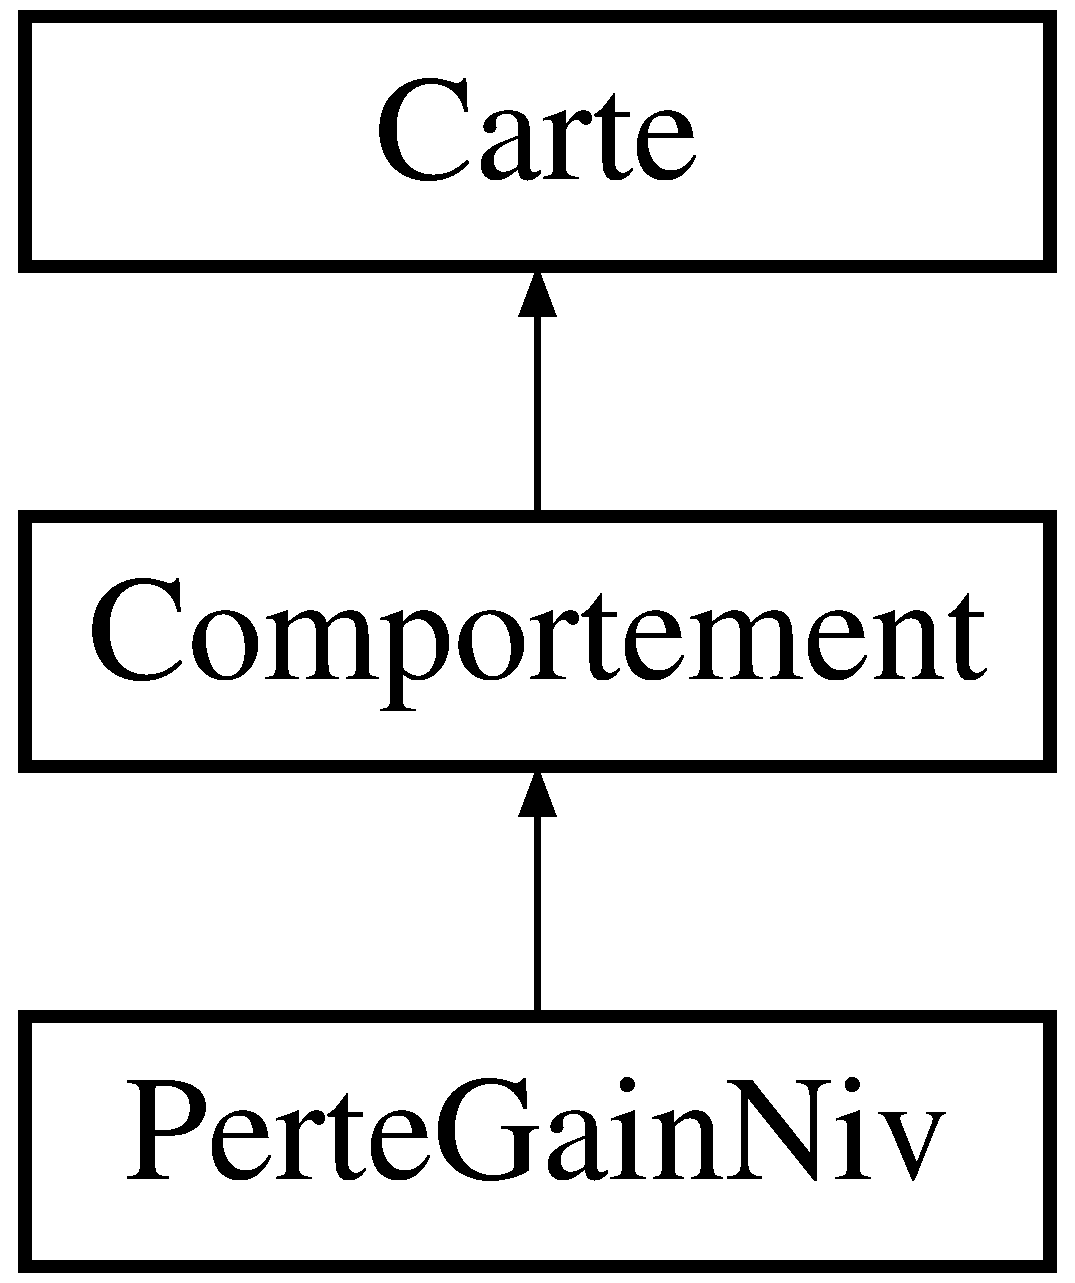
\includegraphics[height=3.000000cm]{class_perte_gain_niv}
\end{center}
\end{figure}
\subsection*{Public Member Functions}
\begin{DoxyCompactItemize}
\item 
\hyperlink{class_perte_gain_niv_a482fc9a3d23b5f0586268f9d100054d3}{Perte\-Gain\-Niv} (\hyperlink{class_carte}{Carte} $\ast$c, int v)
\begin{DoxyCompactList}\small\item\em Constructeur de \hyperlink{class_perte_gain_niv}{Perte\-Gain\-Niv}. \end{DoxyCompactList}\item 
\hypertarget{class_perte_gain_niv_a8250ecb9285f3b109570502dd0434a8c}{\hyperlink{class_perte_gain_niv_a8250ecb9285f3b109570502dd0434a8c}{$\sim$\-Perte\-Gain\-Niv} ()}\label{class_perte_gain_niv_a8250ecb9285f3b109570502dd0434a8c}

\begin{DoxyCompactList}\small\item\em Destructeur de \hyperlink{class_perte_gain_niv}{Perte\-Gain\-Niv}. \end{DoxyCompactList}\item 
virtual void \hyperlink{class_perte_gain_niv_ad72efe1c526391084768a500bb1ae4fa}{appliquer} (\hyperlink{class_personnage}{Personnage} $\ast$p)
\begin{DoxyCompactList}\small\item\em applique le comportement de la carte \end{DoxyCompactList}\end{DoxyCompactItemize}
\subsection*{Additional Inherited Members}


\subsection{Constructor \& Destructor Documentation}
\hypertarget{class_perte_gain_niv_a482fc9a3d23b5f0586268f9d100054d3}{\index{Perte\-Gain\-Niv@{Perte\-Gain\-Niv}!Perte\-Gain\-Niv@{Perte\-Gain\-Niv}}
\index{Perte\-Gain\-Niv@{Perte\-Gain\-Niv}!PerteGainNiv@{Perte\-Gain\-Niv}}
\subsubsection[{Perte\-Gain\-Niv}]{\setlength{\rightskip}{0pt plus 5cm}Perte\-Gain\-Niv\-::\-Perte\-Gain\-Niv (
\begin{DoxyParamCaption}
\item[{{\bf Carte} $\ast$}]{c, }
\item[{int}]{v}
\end{DoxyParamCaption}
)}}\label{class_perte_gain_niv_a482fc9a3d23b5f0586268f9d100054d3}


Constructeur de \hyperlink{class_perte_gain_niv}{Perte\-Gain\-Niv}. 


\begin{DoxyParams}{Parameters}
{\em c} & \hyperlink{class_carte}{Carte} décorée \\
\hline
{\em valeur} & Valeur du comportement \\
\hline
\end{DoxyParams}


\subsection{Member Function Documentation}
\hypertarget{class_perte_gain_niv_ad72efe1c526391084768a500bb1ae4fa}{\index{Perte\-Gain\-Niv@{Perte\-Gain\-Niv}!appliquer@{appliquer}}
\index{appliquer@{appliquer}!PerteGainNiv@{Perte\-Gain\-Niv}}
\subsubsection[{appliquer}]{\setlength{\rightskip}{0pt plus 5cm}void Perte\-Gain\-Niv\-::appliquer (
\begin{DoxyParamCaption}
\item[{{\bf Personnage} $\ast$}]{p}
\end{DoxyParamCaption}
)\hspace{0.3cm}{\ttfamily [virtual]}}}\label{class_perte_gain_niv_ad72efe1c526391084768a500bb1ae4fa}


applique le comportement de la carte 


\begin{DoxyParams}{Parameters}
{\em cible} & du comportement \\
\hline
\end{DoxyParams}


Reimplemented from \hyperlink{class_comportement_ae55149d29c710b0a5a0388cae308024f}{Comportement}.



The documentation for this class was generated from the following files\-:\begin{DoxyCompactItemize}
\item 
\hyperlink{_perte_gain_niv_8hpp}{Perte\-Gain\-Niv.\-hpp}\item 
\hyperlink{_perte_gain_niv_8cpp}{Perte\-Gain\-Niv.\-cpp}\end{DoxyCompactItemize}

\hypertarget{class_perte_obj_max}{\section{Perte\-Obj\-Max Class Reference}
\label{class_perte_obj_max}\index{Perte\-Obj\-Max@{Perte\-Obj\-Max}}
}
Inheritance diagram for Perte\-Obj\-Max\-:\begin{figure}[H]
\begin{center}
\leavevmode
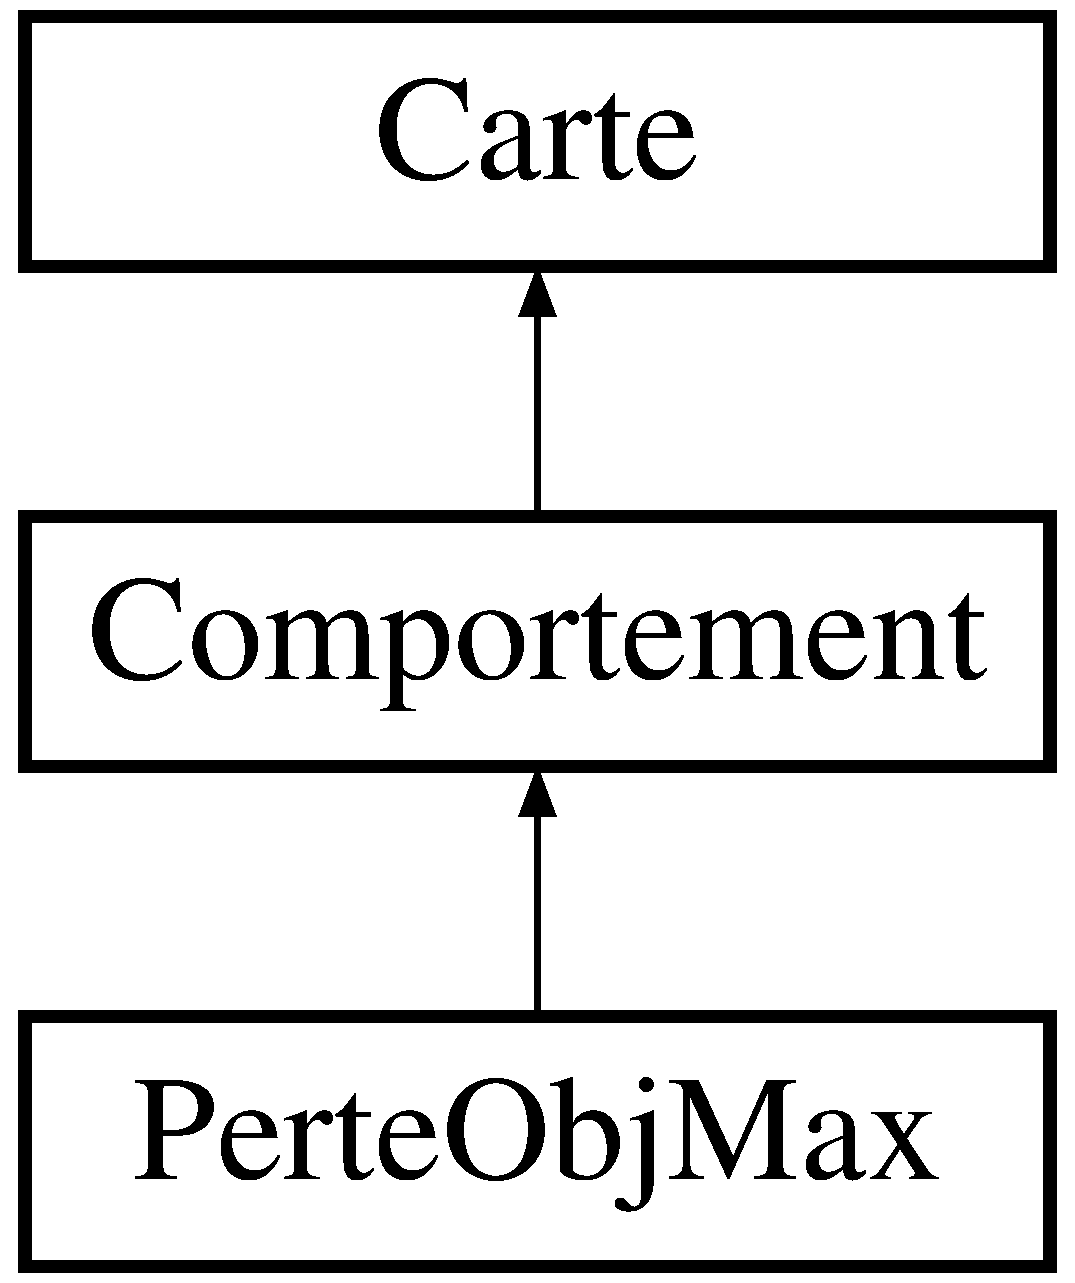
\includegraphics[height=3.000000cm]{class_perte_obj_max}
\end{center}
\end{figure}
\subsection*{Public Member Functions}
\begin{DoxyCompactItemize}
\item 
\hyperlink{class_perte_obj_max_a09e5098794871ff918ada7a0be551a8a}{Perte\-Obj\-Max} (\hyperlink{class_carte}{Carte} $\ast$c, int v)
\begin{DoxyCompactList}\small\item\em Constructeur de \hyperlink{class_perte_obj_max}{Perte\-Obj\-Max}. \end{DoxyCompactList}\item 
\hypertarget{class_perte_obj_max_a4968847588d00d3a4e4d158a960c531c}{\hyperlink{class_perte_obj_max_a4968847588d00d3a4e4d158a960c531c}{$\sim$\-Perte\-Obj\-Max} ()}\label{class_perte_obj_max_a4968847588d00d3a4e4d158a960c531c}

\begin{DoxyCompactList}\small\item\em Destructeur de \hyperlink{class_perte_obj_max}{Perte\-Obj\-Max}. \end{DoxyCompactList}\item 
virtual void \hyperlink{class_perte_obj_max_a929e1c6370247feb937ae1835648a441}{appliquer} (\hyperlink{class_personnage}{Personnage} $\ast$p)
\begin{DoxyCompactList}\small\item\em applique le comportement de la carte \end{DoxyCompactList}\end{DoxyCompactItemize}
\subsection*{Additional Inherited Members}


\subsection{Constructor \& Destructor Documentation}
\hypertarget{class_perte_obj_max_a09e5098794871ff918ada7a0be551a8a}{\index{Perte\-Obj\-Max@{Perte\-Obj\-Max}!Perte\-Obj\-Max@{Perte\-Obj\-Max}}
\index{Perte\-Obj\-Max@{Perte\-Obj\-Max}!PerteObjMax@{Perte\-Obj\-Max}}
\subsubsection[{Perte\-Obj\-Max}]{\setlength{\rightskip}{0pt plus 5cm}Perte\-Obj\-Max\-::\-Perte\-Obj\-Max (
\begin{DoxyParamCaption}
\item[{{\bf Carte} $\ast$}]{c, }
\item[{int}]{v}
\end{DoxyParamCaption}
)}}\label{class_perte_obj_max_a09e5098794871ff918ada7a0be551a8a}


Constructeur de \hyperlink{class_perte_obj_max}{Perte\-Obj\-Max}. 


\begin{DoxyParams}{Parameters}
{\em c} & \hyperlink{class_carte}{Carte} décorée \\
\hline
{\em valeur} & Valeur du comportement \\
\hline
\end{DoxyParams}


\subsection{Member Function Documentation}
\hypertarget{class_perte_obj_max_a929e1c6370247feb937ae1835648a441}{\index{Perte\-Obj\-Max@{Perte\-Obj\-Max}!appliquer@{appliquer}}
\index{appliquer@{appliquer}!PerteObjMax@{Perte\-Obj\-Max}}
\subsubsection[{appliquer}]{\setlength{\rightskip}{0pt plus 5cm}void Perte\-Obj\-Max\-::appliquer (
\begin{DoxyParamCaption}
\item[{{\bf Personnage} $\ast$}]{p}
\end{DoxyParamCaption}
)\hspace{0.3cm}{\ttfamily [virtual]}}}\label{class_perte_obj_max_a929e1c6370247feb937ae1835648a441}


applique le comportement de la carte 


\begin{DoxyParams}{Parameters}
{\em cible} & du comportement \\
\hline
\end{DoxyParams}


Reimplemented from \hyperlink{class_comportement_ae55149d29c710b0a5a0388cae308024f}{Comportement}.



The documentation for this class was generated from the following files\-:\begin{DoxyCompactItemize}
\item 
\hyperlink{_perte_obj_max_8hpp}{Perte\-Obj\-Max.\-hpp}\item 
\hyperlink{_perte_obj_max_8cpp}{Perte\-Obj\-Max.\-cpp}\end{DoxyCompactItemize}

\hypertarget{class_porte}{\section{Porte Class Reference}
\label{class_porte}\index{Porte@{Porte}}
}
Inheritance diagram for Porte\-:\begin{figure}[H]
\begin{center}
\leavevmode
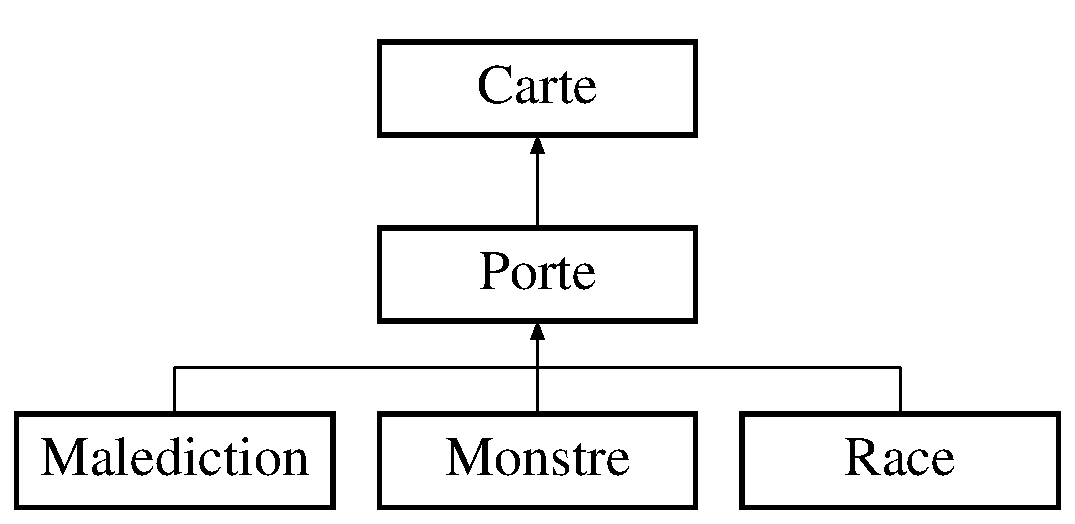
\includegraphics[height=3.000000cm]{class_porte}
\end{center}
\end{figure}
\subsection*{Public Member Functions}
\begin{DoxyCompactItemize}
\item 
\hyperlink{class_porte_af7c81d2889785a946b4074b97365f0d9}{Porte} (int id, std\-::string \hyperlink{class_carte_a46bff2b84b76b6b94b2eaa3fe813ec69}{nom}, std\-::string \hyperlink{class_carte_a5f2acc07fa281fb6d4467c00bd4b1614}{description})
\begin{DoxyCompactList}\small\item\em Constructeur de \hyperlink{class_porte}{Porte}. \end{DoxyCompactList}\item 
\hypertarget{class_porte_a7b82ccac24bfd8b7fa701f7601328d6c}{virtual \hyperlink{class_porte_a7b82ccac24bfd8b7fa701f7601328d6c}{$\sim$\-Porte} ()}\label{class_porte_a7b82ccac24bfd8b7fa701f7601328d6c}

\begin{DoxyCompactList}\small\item\em Destructeur de \hyperlink{class_porte}{Porte}. \end{DoxyCompactList}\item 
bool \hyperlink{class_porte_a8a7e6c7c6b1d94b157b2229a6e32ac93}{est\-Porte} ()
\begin{DoxyCompactList}\small\item\em Renvoie vrai si c'est une \hyperlink{class_porte}{Porte}. \end{DoxyCompactList}\end{DoxyCompactItemize}
\subsection*{Additional Inherited Members}


\subsection{Constructor \& Destructor Documentation}
\hypertarget{class_porte_af7c81d2889785a946b4074b97365f0d9}{\index{Porte@{Porte}!Porte@{Porte}}
\index{Porte@{Porte}!Porte@{Porte}}
\subsubsection[{Porte}]{\setlength{\rightskip}{0pt plus 5cm}Porte\-::\-Porte (
\begin{DoxyParamCaption}
\item[{int}]{id, }
\item[{std\-::string}]{n, }
\item[{std\-::string}]{d}
\end{DoxyParamCaption}
)}}\label{class_porte_af7c81d2889785a946b4074b97365f0d9}


Constructeur de \hyperlink{class_porte}{Porte}. 


\begin{DoxyParams}{Parameters}
{\em id} & Identifiant de la carte \\
\hline
{\em nom} & nom de la carte \\
\hline
{\em description} & description de la carte \\
\hline
\end{DoxyParams}


\subsection{Member Function Documentation}
\hypertarget{class_porte_a8a7e6c7c6b1d94b157b2229a6e32ac93}{\index{Porte@{Porte}!est\-Porte@{est\-Porte}}
\index{est\-Porte@{est\-Porte}!Porte@{Porte}}
\subsubsection[{est\-Porte}]{\setlength{\rightskip}{0pt plus 5cm}bool Porte\-::est\-Porte (
\begin{DoxyParamCaption}
{}
\end{DoxyParamCaption}
)\hspace{0.3cm}{\ttfamily [virtual]}}}\label{class_porte_a8a7e6c7c6b1d94b157b2229a6e32ac93}


Renvoie vrai si c'est une \hyperlink{class_porte}{Porte}. 

\begin{DoxyReturn}{Returns}
vrai si c'est une \hyperlink{class_porte}{Porte}, Faux sinon 
\end{DoxyReturn}


Reimplemented from \hyperlink{class_carte_af0156ad1b4b87414df65caddd310212a}{Carte}.



The documentation for this class was generated from the following files\-:\begin{DoxyCompactItemize}
\item 
\hyperlink{_porte_8hpp}{Porte.\-hpp}\item 
\hyperlink{_porte_8cpp}{Porte.\-cpp}\end{DoxyCompactItemize}

\hypertarget{class_potion}{\section{Potion Class Reference}
\label{class_potion}\index{Potion@{Potion}}
}
Inheritance diagram for Potion\-:\begin{figure}[H]
\begin{center}
\leavevmode
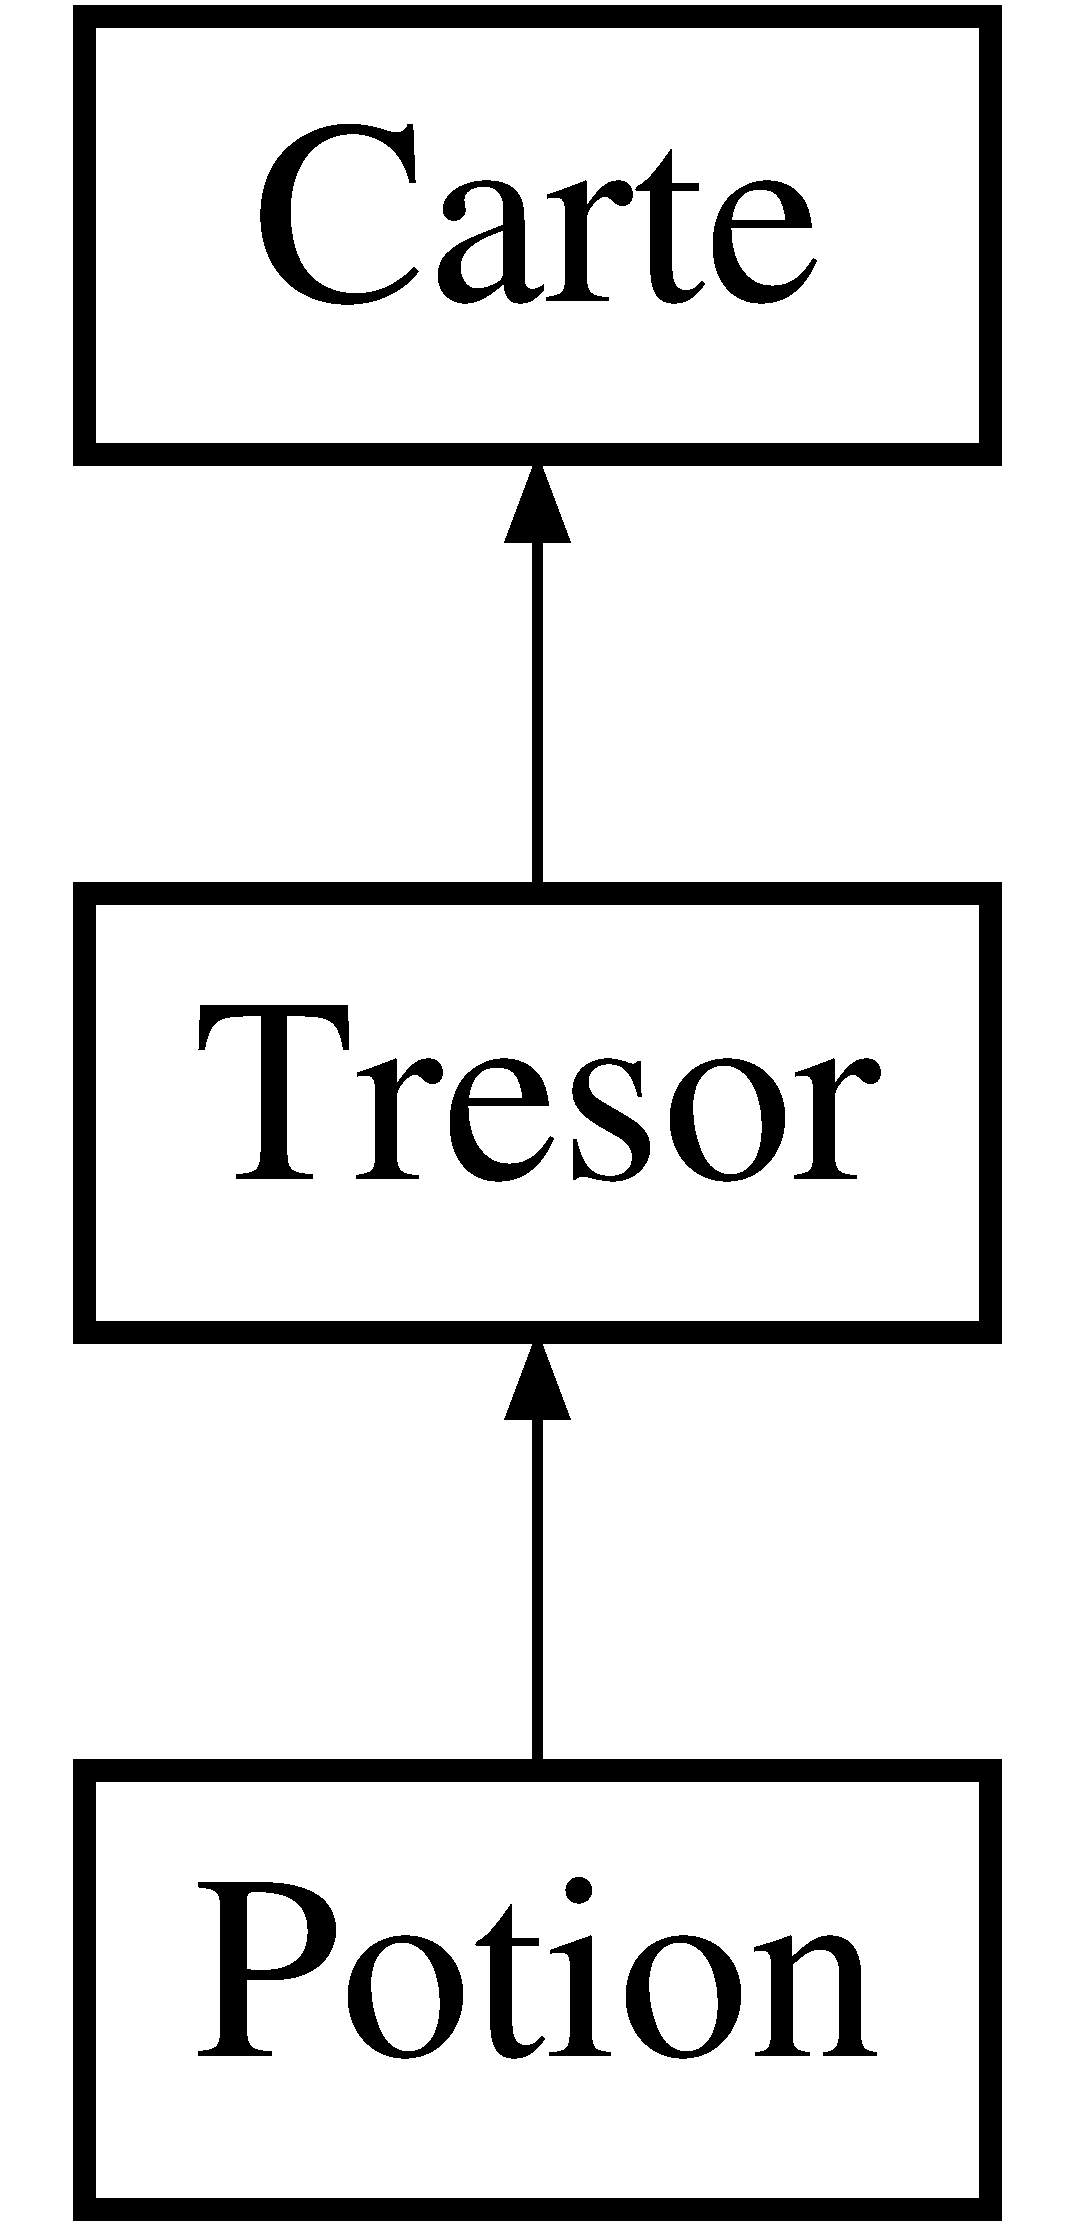
\includegraphics[height=3.000000cm]{class_potion}
\end{center}
\end{figure}
\subsection*{Public Member Functions}
\begin{DoxyCompactItemize}
\item 
\hyperlink{class_potion_a6a6ade33a2c7c7502168594be6c15747}{Potion} (int id, std\-::string n, std\-::string d, int p)
\begin{DoxyCompactList}\small\item\em Constructeur de \hyperlink{class_tresor}{Tresor}. \end{DoxyCompactList}\item 
\hypertarget{class_potion_a8730c8052ec698171885bb5dacda9cca}{virtual \hyperlink{class_potion_a8730c8052ec698171885bb5dacda9cca}{$\sim$\-Potion} ()}\label{class_potion_a8730c8052ec698171885bb5dacda9cca}

\begin{DoxyCompactList}\small\item\em Destructeur de \hyperlink{class_potion}{Potion}. \end{DoxyCompactList}\item 
bool \hyperlink{class_potion_aa04fc4873583e7b1f90416b226edbe06}{est\-Potion} ()
\begin{DoxyCompactList}\small\item\em Renvoie vrai si c'est une \hyperlink{class_potion}{Potion}. \end{DoxyCompactList}\end{DoxyCompactItemize}
\subsection*{Additional Inherited Members}


\subsection{Constructor \& Destructor Documentation}
\hypertarget{class_potion_a6a6ade33a2c7c7502168594be6c15747}{\index{Potion@{Potion}!Potion@{Potion}}
\index{Potion@{Potion}!Potion@{Potion}}
\subsubsection[{Potion}]{\setlength{\rightskip}{0pt plus 5cm}Potion\-::\-Potion (
\begin{DoxyParamCaption}
\item[{int}]{id, }
\item[{std\-::string}]{n, }
\item[{std\-::string}]{d, }
\item[{int}]{p}
\end{DoxyParamCaption}
)}}\label{class_potion_a6a6ade33a2c7c7502168594be6c15747}


Constructeur de \hyperlink{class_tresor}{Tresor}. 


\begin{DoxyParams}{Parameters}
{\em id} & Identifiant de la carte \\
\hline
{\em n} & nom de la carte \\
\hline
{\em d} & description de la carte \\
\hline
{\em p} & prix de la carte \\
\hline
\end{DoxyParams}


\subsection{Member Function Documentation}
\hypertarget{class_potion_aa04fc4873583e7b1f90416b226edbe06}{\index{Potion@{Potion}!est\-Potion@{est\-Potion}}
\index{est\-Potion@{est\-Potion}!Potion@{Potion}}
\subsubsection[{est\-Potion}]{\setlength{\rightskip}{0pt plus 5cm}bool Potion\-::est\-Potion (
\begin{DoxyParamCaption}
{}
\end{DoxyParamCaption}
)\hspace{0.3cm}{\ttfamily [virtual]}}}\label{class_potion_aa04fc4873583e7b1f90416b226edbe06}


Renvoie vrai si c'est une \hyperlink{class_potion}{Potion}. 

\begin{DoxyReturn}{Returns}
vrai si c'est une \hyperlink{class_potion}{Potion}, Faux sinon 
\end{DoxyReturn}


Reimplemented from \hyperlink{class_carte_a3be68ed1ee99d835cd27148e456e5b9c}{Carte}.



The documentation for this class was generated from the following files\-:\begin{DoxyCompactItemize}
\item 
\hyperlink{_potion_8hpp}{Potion.\-hpp}\item 
\hyperlink{_potion_8cpp}{Potion.\-cpp}\end{DoxyCompactItemize}

\hypertarget{class_race}{\section{Race Class Reference}
\label{class_race}\index{Race@{Race}}
}
Inheritance diagram for Race\-:\begin{figure}[H]
\begin{center}
\leavevmode
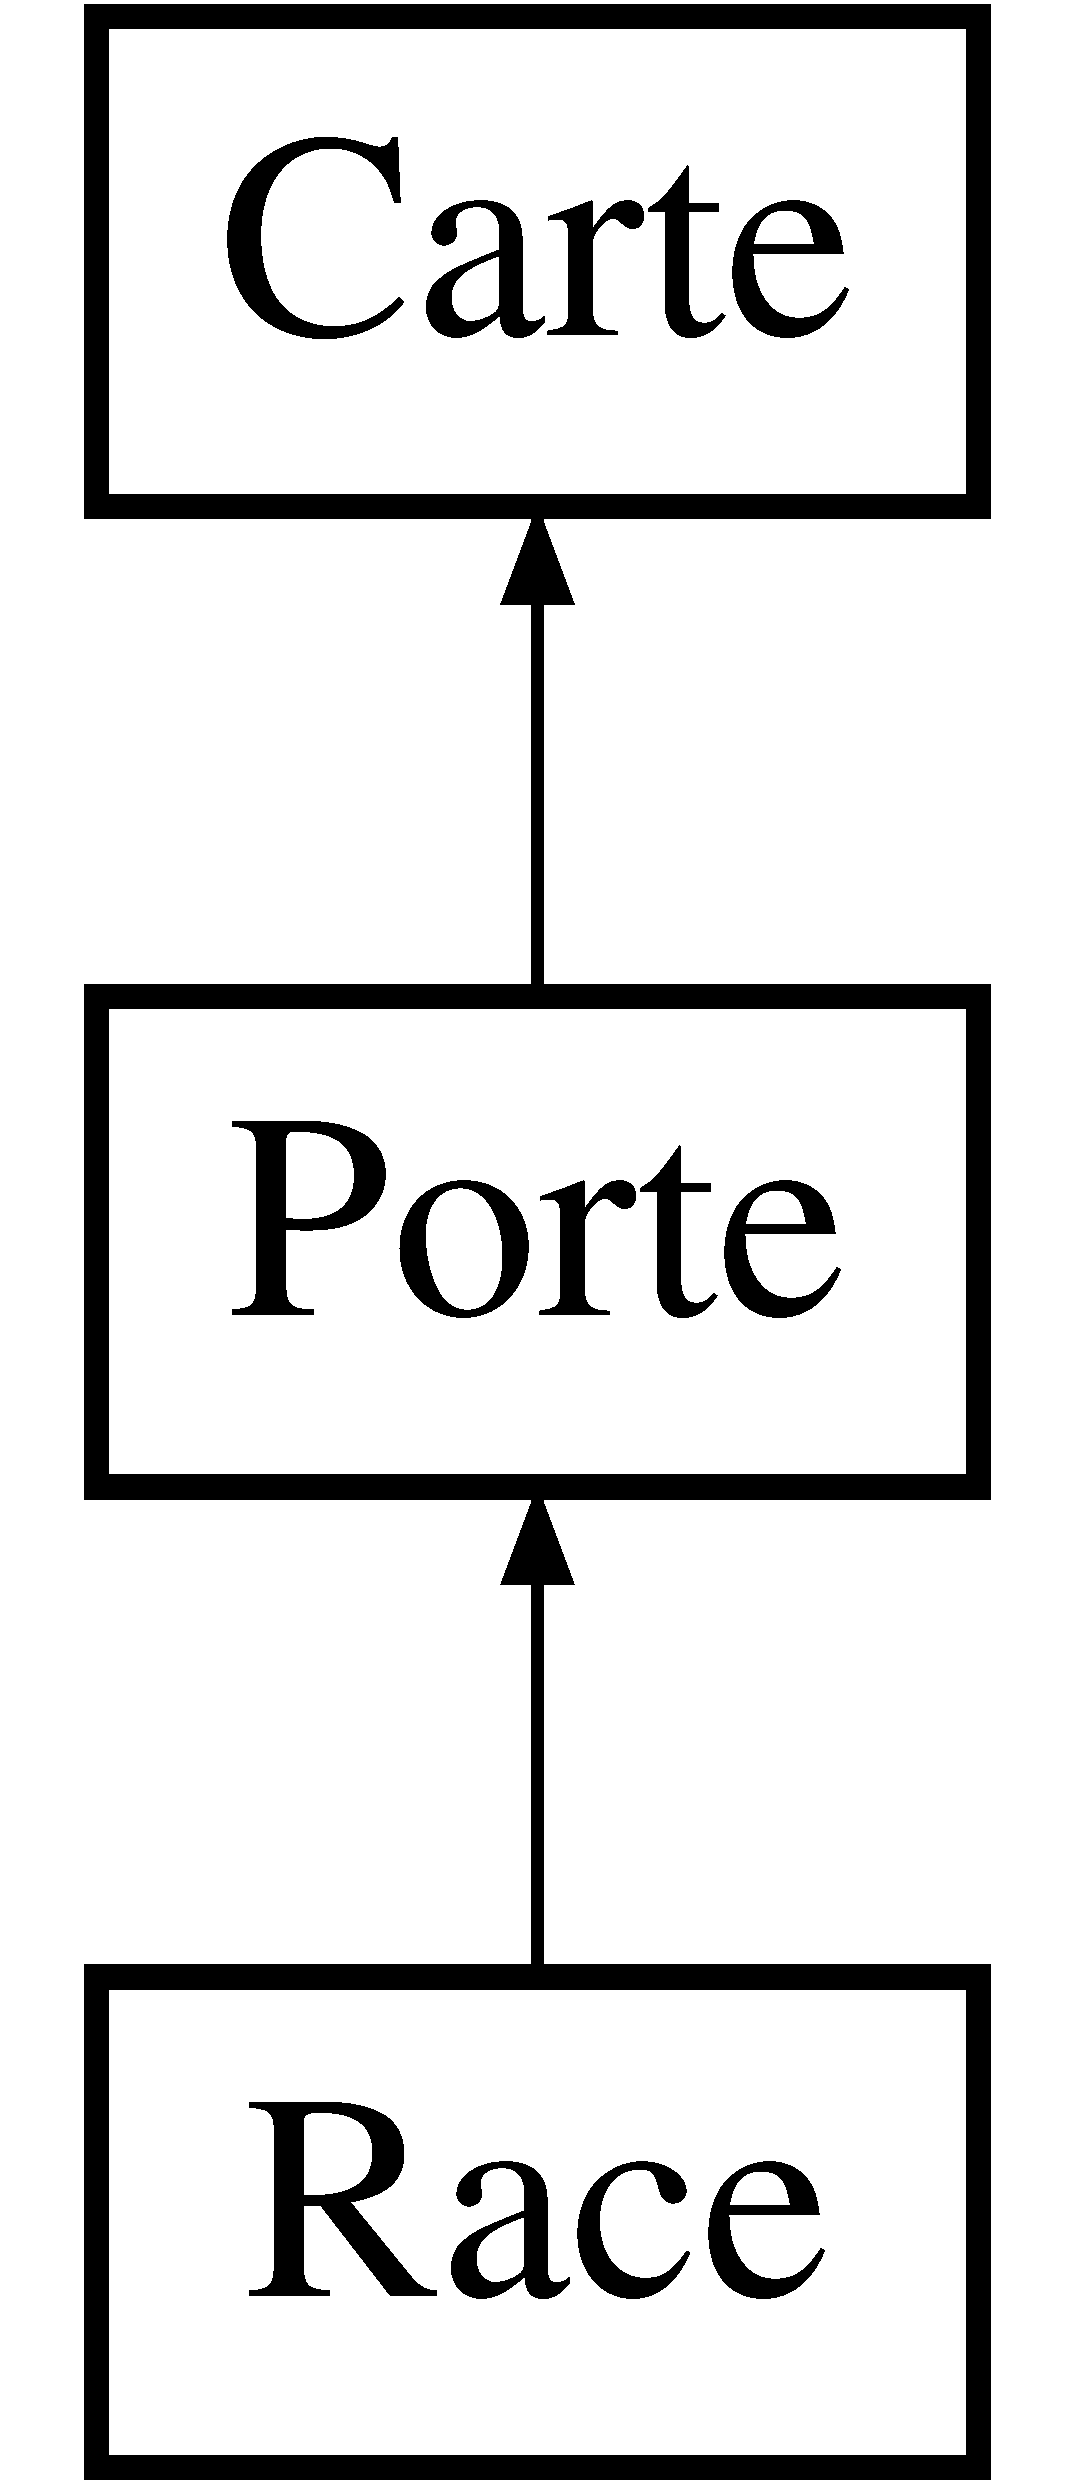
\includegraphics[height=3.000000cm]{class_race}
\end{center}
\end{figure}
\subsection*{Public Member Functions}
\begin{DoxyCompactItemize}
\item 
\hyperlink{class_race_a0df40698a7c2542ab077d3c656e13fab}{Race} (int id, std\-::string \hyperlink{class_carte_a46bff2b84b76b6b94b2eaa3fe813ec69}{nom}, std\-::string \hyperlink{class_carte_a5f2acc07fa281fb6d4467c00bd4b1614}{description})
\begin{DoxyCompactList}\small\item\em Constructeur de \hyperlink{class_race}{Race}. \end{DoxyCompactList}\item 
\hypertarget{class_race_ad6bfb0bc96485e23b3bf45d794b5b536}{\hyperlink{class_race_ad6bfb0bc96485e23b3bf45d794b5b536}{$\sim$\-Race} ()}\label{class_race_ad6bfb0bc96485e23b3bf45d794b5b536}

\begin{DoxyCompactList}\small\item\em Destructeur de \hyperlink{class_race}{Race}. \end{DoxyCompactList}\item 
\hypertarget{class_race_a2f6e239a9ef0271c376660e692a553db}{void \hyperlink{class_race_a2f6e239a9ef0271c376660e692a553db}{poser} (\hyperlink{class_joueur}{Joueur} $\ast$j)}\label{class_race_a2f6e239a9ef0271c376660e692a553db}

\begin{DoxyCompactList}\small\item\em Applique le comportement de la carte. \end{DoxyCompactList}\item 
bool \hyperlink{class_race_a4d583fa670a0c3666715b89f86935060}{est\-Race} ()
\begin{DoxyCompactList}\small\item\em Renvoie vrai si c'est une \hyperlink{class_race}{Race}. \end{DoxyCompactList}\end{DoxyCompactItemize}
\subsection*{Additional Inherited Members}


\subsection{Constructor \& Destructor Documentation}
\hypertarget{class_race_a0df40698a7c2542ab077d3c656e13fab}{\index{Race@{Race}!Race@{Race}}
\index{Race@{Race}!Race@{Race}}
\subsubsection[{Race}]{\setlength{\rightskip}{0pt plus 5cm}Race\-::\-Race (
\begin{DoxyParamCaption}
\item[{int}]{id, }
\item[{std\-::string}]{n, }
\item[{std\-::string}]{d}
\end{DoxyParamCaption}
)}}\label{class_race_a0df40698a7c2542ab077d3c656e13fab}


Constructeur de \hyperlink{class_race}{Race}. 


\begin{DoxyParams}{Parameters}
{\em id} & Identifiant de la carte \\
\hline
{\em nom} & nom de la carte \\
\hline
{\em description} & description de la carte \\
\hline
\end{DoxyParams}


\subsection{Member Function Documentation}
\hypertarget{class_race_a4d583fa670a0c3666715b89f86935060}{\index{Race@{Race}!est\-Race@{est\-Race}}
\index{est\-Race@{est\-Race}!Race@{Race}}
\subsubsection[{est\-Race}]{\setlength{\rightskip}{0pt plus 5cm}bool Race\-::est\-Race (
\begin{DoxyParamCaption}
{}
\end{DoxyParamCaption}
)\hspace{0.3cm}{\ttfamily [virtual]}}}\label{class_race_a4d583fa670a0c3666715b89f86935060}


Renvoie vrai si c'est une \hyperlink{class_race}{Race}. 

\begin{DoxyReturn}{Returns}
vrai si c'est une \hyperlink{class_race}{Race}, Faux sinon 
\end{DoxyReturn}


Reimplemented from \hyperlink{class_carte_acbac53716e6285801ca151aa177fc699}{Carte}.



The documentation for this class was generated from the following files\-:\begin{DoxyCompactItemize}
\item 
\hyperlink{_race_8hpp}{Race.\-hpp}\item 
\hyperlink{_race_8cpp}{Race.\-cpp}\end{DoxyCompactItemize}

\hypertarget{class_tresor}{\section{Tresor Class Reference}
\label{class_tresor}\index{Tresor@{Tresor}}
}
Inheritance diagram for Tresor\-:\begin{figure}[H]
\begin{center}
\leavevmode
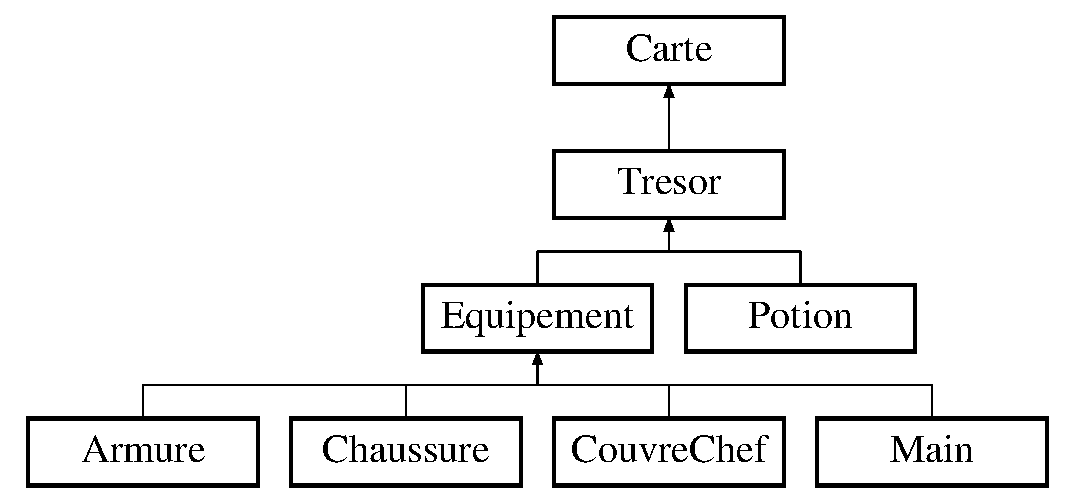
\includegraphics[height=4.000000cm]{class_tresor}
\end{center}
\end{figure}
\subsection*{Public Member Functions}
\begin{DoxyCompactItemize}
\item 
\hyperlink{class_tresor_a9552fed8f2ce245f4baf31ed1e2512ba}{Tresor} (int id, std\-::string n, std\-::string d, int p)
\begin{DoxyCompactList}\small\item\em Constructeur de \hyperlink{class_tresor}{Tresor}. \end{DoxyCompactList}\item 
\hypertarget{class_tresor_ac78eeccd0ea7b5ef56e3fc9585b0c8f2}{virtual \hyperlink{class_tresor_ac78eeccd0ea7b5ef56e3fc9585b0c8f2}{$\sim$\-Tresor} ()}\label{class_tresor_ac78eeccd0ea7b5ef56e3fc9585b0c8f2}

\begin{DoxyCompactList}\small\item\em Destructeur de \hyperlink{class_tresor}{Tresor}. \end{DoxyCompactList}\item 
int \hyperlink{class_tresor_a028507292b291321832bccb4622efeed}{get\-Prix} ()
\begin{DoxyCompactList}\small\item\em Renvoie le prix de la carte. \end{DoxyCompactList}\item 
bool \hyperlink{class_tresor_ade57ffa16e80824293ca128f18b9c648}{est\-Tresor} ()
\begin{DoxyCompactList}\small\item\em Renvoie vrai si c'est une \hyperlink{class_tresor}{Tresor}. \end{DoxyCompactList}\end{DoxyCompactItemize}
\subsection*{Protected Attributes}
\begin{DoxyCompactItemize}
\item 
int \hyperlink{class_tresor_aa645398268d08ff8620c404612578100}{prix}
\end{DoxyCompactItemize}


\subsection{Constructor \& Destructor Documentation}
\hypertarget{class_tresor_a9552fed8f2ce245f4baf31ed1e2512ba}{\index{Tresor@{Tresor}!Tresor@{Tresor}}
\index{Tresor@{Tresor}!Tresor@{Tresor}}
\subsubsection[{Tresor}]{\setlength{\rightskip}{0pt plus 5cm}Tresor\-::\-Tresor (
\begin{DoxyParamCaption}
\item[{int}]{id, }
\item[{std\-::string}]{n, }
\item[{std\-::string}]{d, }
\item[{int}]{p}
\end{DoxyParamCaption}
)}}\label{class_tresor_a9552fed8f2ce245f4baf31ed1e2512ba}


Constructeur de \hyperlink{class_tresor}{Tresor}. 


\begin{DoxyParams}{Parameters}
{\em id} & Identifiant de la carte \\
\hline
{\em n} & nom de la carte \\
\hline
{\em d} & description de la carte \\
\hline
{\em p} & prix de la carte \\
\hline
\end{DoxyParams}


\subsection{Member Function Documentation}
\hypertarget{class_tresor_ade57ffa16e80824293ca128f18b9c648}{\index{Tresor@{Tresor}!est\-Tresor@{est\-Tresor}}
\index{est\-Tresor@{est\-Tresor}!Tresor@{Tresor}}
\subsubsection[{est\-Tresor}]{\setlength{\rightskip}{0pt plus 5cm}bool Tresor\-::est\-Tresor (
\begin{DoxyParamCaption}
{}
\end{DoxyParamCaption}
)\hspace{0.3cm}{\ttfamily [virtual]}}}\label{class_tresor_ade57ffa16e80824293ca128f18b9c648}


Renvoie vrai si c'est une \hyperlink{class_tresor}{Tresor}. 

\begin{DoxyReturn}{Returns}
vrai si c'est un tr�sor, Faux sinon 
\end{DoxyReturn}


Reimplemented from \hyperlink{class_carte_a5fcbed672fcb0141ac2349db64d82385}{Carte}.

\hypertarget{class_tresor_a028507292b291321832bccb4622efeed}{\index{Tresor@{Tresor}!get\-Prix@{get\-Prix}}
\index{get\-Prix@{get\-Prix}!Tresor@{Tresor}}
\subsubsection[{get\-Prix}]{\setlength{\rightskip}{0pt plus 5cm}int Tresor\-::get\-Prix (
\begin{DoxyParamCaption}
{}
\end{DoxyParamCaption}
)}}\label{class_tresor_a028507292b291321832bccb4622efeed}


Renvoie le prix de la carte. 

\begin{DoxyReturn}{Returns}
prix de la carte 
\end{DoxyReturn}


\subsection{Member Data Documentation}
\hypertarget{class_tresor_aa645398268d08ff8620c404612578100}{\index{Tresor@{Tresor}!prix@{prix}}
\index{prix@{prix}!Tresor@{Tresor}}
\subsubsection[{prix}]{\setlength{\rightskip}{0pt plus 5cm}int Tresor\-::prix\hspace{0.3cm}{\ttfamily [protected]}}}\label{class_tresor_aa645398268d08ff8620c404612578100}
prix de la carte 

The documentation for this class was generated from the following files\-:\begin{DoxyCompactItemize}
\item 
\hyperlink{_tresor_8hpp}{Tresor.\-hpp}\item 
\hyperlink{_tresor_8cpp}{Tresor.\-cpp}\end{DoxyCompactItemize}

\chapter{File Documentation}
\hypertarget{_armure_8hpp}{\section{Armure.\-hpp File Reference}
\label{_armure_8hpp}\index{Armure.\-hpp@{Armure.\-hpp}}
}


declaration classe \hyperlink{class_armure}{Armure}  


{\ttfamily \#include \char`\"{}../\-Equipement.\-hpp\char`\"{}}\\*
\subsection*{Classes}
\begin{DoxyCompactItemize}
\item 
class \hyperlink{class_armure}{Armure}
\end{DoxyCompactItemize}


\subsection{Detailed Description}
declaration classe \hyperlink{class_armure}{Armure} \begin{DoxyAuthor}{Author}
Bois Cédric Le Corvec Quentin 
\end{DoxyAuthor}
\begin{DoxyDate}{Date}
Octobre 2014 
\end{DoxyDate}

\hypertarget{_attente_8cpp}{\section{Attente.\-cpp File Reference}
\label{_attente_8cpp}\index{Attente.\-cpp@{Attente.\-cpp}}
}


implémentation classe \hyperlink{class_attente}{Attente}  


{\ttfamily \#include \char`\"{}Attente.\-hpp\char`\"{}}\\*


\subsection{Detailed Description}
implémentation classe \hyperlink{class_attente}{Attente} \begin{DoxyAuthor}{Author}
Bois Cédric Le Corvec Quentin 
\end{DoxyAuthor}
\begin{DoxyDate}{Date}
Octobre 2014 
\end{DoxyDate}

\hypertarget{_attente_8hpp}{\section{Attente.\-hpp File Reference}
\label{_attente_8hpp}\index{Attente.\-hpp@{Attente.\-hpp}}
}


declaration classe \hyperlink{class_attente}{Attente}  


{\ttfamily \#include \char`\"{}../\-Etat\-Joueur.\-hpp\char`\"{}}\\*
{\ttfamily \#include \char`\"{}../../\-Joueur.\-hpp\char`\"{}}\\*
\subsection*{Classes}
\begin{DoxyCompactItemize}
\item 
class \hyperlink{class_attente}{Attente}
\end{DoxyCompactItemize}


\subsection{Detailed Description}
declaration classe \hyperlink{class_attente}{Attente} \begin{DoxyAuthor}{Author}
Bois Cédric Le Corvec Quentin 
\end{DoxyAuthor}
\begin{DoxyDate}{Date}
Octobre 2014 
\end{DoxyDate}

\hypertarget{_bagarre_8cpp}{\section{Bagarre.\-cpp File Reference}
\label{_bagarre_8cpp}\index{Bagarre.\-cpp@{Bagarre.\-cpp}}
}


implémentation classe \hyperlink{class_bagarre}{Bagarre}  


{\ttfamily \#include \char`\"{}Bagarre.\-hpp\char`\"{}}\\*


\subsection{Detailed Description}
implémentation classe \hyperlink{class_bagarre}{Bagarre} \begin{DoxyAuthor}{Author}
Bois Cédric Le Corvec Quentin 
\end{DoxyAuthor}
\begin{DoxyDate}{Date}
Octobre 2014 
\end{DoxyDate}

\hypertarget{_bagarre_8hpp}{\section{Bagarre.\-hpp File Reference}
\label{_bagarre_8hpp}\index{Bagarre.\-hpp@{Bagarre.\-hpp}}
}


declaration classe \hyperlink{class_bagarre}{Bagarre}  


{\ttfamily \#include \char`\"{}../../../../\-Carte/\-Carte.\-hpp\char`\"{}}\\*
{\ttfamily \#include $<$time.\-h$>$}\\*
{\ttfamily \#include $<$stdlib.\-h$>$}\\*
{\ttfamily \#include \char`\"{}../\-Etat\-Joueur.\-hpp\char`\"{}}\\*
{\ttfamily \#include \char`\"{}../../\-Joueur.\-hpp\char`\"{}}\\*
{\ttfamily \#include \char`\"{}../../../../\-Carte/\-Tresor/\-Equipement/\-Equipement.\-hpp\char`\"{}}\\*
\subsection*{Classes}
\begin{DoxyCompactItemize}
\item 
class \hyperlink{class_bagarre}{Bagarre}
\end{DoxyCompactItemize}


\subsection{Detailed Description}
declaration classe \hyperlink{class_bagarre}{Bagarre} \begin{DoxyAuthor}{Author}
Bois Cédric Le Corvec Quentin 
\end{DoxyAuthor}
\begin{DoxyDate}{Date}
Octobre 2014 
\end{DoxyDate}

\hypertarget{_carte_8cpp}{\section{Carte.\-cpp File Reference}
\label{_carte_8cpp}\index{Carte.\-cpp@{Carte.\-cpp}}
}


implementation classe \hyperlink{class_carte}{Carte}  


{\ttfamily \#include \char`\"{}Carte.\-hpp\char`\"{}}\\*


\subsection{Detailed Description}
implementation classe \hyperlink{class_carte}{Carte} \begin{DoxyAuthor}{Author}
Bois C�dric Le Corvec Quentin 
\end{DoxyAuthor}
\begin{DoxyDate}{Date}
Octobre 2014 
\end{DoxyDate}

\hypertarget{_carte_8hpp}{\section{Carte.\-hpp File Reference}
\label{_carte_8hpp}\index{Carte.\-hpp@{Carte.\-hpp}}
}


d�claration classe \hyperlink{class_carte}{Carte}  


{\ttfamily \#include $<$string$>$}\\*
\subsection*{Classes}
\begin{DoxyCompactItemize}
\item 
class \hyperlink{class_carte}{Carte}
\end{DoxyCompactItemize}


\subsection{Detailed Description}
d�claration classe \hyperlink{class_carte}{Carte} \begin{DoxyAuthor}{Author}
Bois C�dric Le Corvec Quentin 
\end{DoxyAuthor}
\begin{DoxyDate}{Date}
Octobre 2014 
\end{DoxyDate}

\hypertarget{_carte_sup_main_8cpp}{\section{Carte\-Sup\-Main.\-cpp File Reference}
\label{_carte_sup_main_8cpp}\index{Carte\-Sup\-Main.\-cpp@{Carte\-Sup\-Main.\-cpp}}
}


implementation classe \hyperlink{class_carte_sup_main}{Carte\-Sup\-Main}  


{\ttfamily \#include \char`\"{}Carte\-Sup\-Main.\-hpp\char`\"{}}\\*


\subsection{Detailed Description}
implementation classe \hyperlink{class_carte_sup_main}{Carte\-Sup\-Main} \begin{DoxyAuthor}{Author}
Bois Cédric Le Corvec Quentin 
\end{DoxyAuthor}
\begin{DoxyDate}{Date}
Octobre 2014 
\end{DoxyDate}

\hypertarget{_carte_sup_main_8hpp}{\section{Carte\-Sup\-Main.\-hpp File Reference}
\label{_carte_sup_main_8hpp}\index{Carte\-Sup\-Main.\-hpp@{Carte\-Sup\-Main.\-hpp}}
}


declaration classe \hyperlink{class_carte_sup_main}{Carte\-Sup\-Main}  


{\ttfamily \#include \char`\"{}../../../\-Personnage/\-Joueur/\-Joueur.\-hpp\char`\"{}}\\*
{\ttfamily \#include \char`\"{}../\-Comportement.\-hpp\char`\"{}}\\*
\subsection*{Classes}
\begin{DoxyCompactItemize}
\item 
class \hyperlink{class_carte_sup_main}{Carte\-Sup\-Main}
\end{DoxyCompactItemize}


\subsection{Detailed Description}
declaration classe \hyperlink{class_carte_sup_main}{Carte\-Sup\-Main} \begin{DoxyAuthor}{Author}
Bois Cédric Le Corvec Quentin 
\end{DoxyAuthor}
\begin{DoxyDate}{Date}
Octobre 2014 
\end{DoxyDate}

\hypertarget{_chaussure_8hpp}{\section{Chaussure.\-hpp File Reference}
\label{_chaussure_8hpp}\index{Chaussure.\-hpp@{Chaussure.\-hpp}}
}


declaration classe \hyperlink{class_chaussure}{Chaussure}  


{\ttfamily \#include \char`\"{}../\-Equipement.\-hpp\char`\"{}}\\*
\subsection*{Classes}
\begin{DoxyCompactItemize}
\item 
class \hyperlink{class_chaussure}{Chaussure}
\end{DoxyCompactItemize}


\subsection{Detailed Description}
declaration classe \hyperlink{class_chaussure}{Chaussure} \begin{DoxyAuthor}{Author}
Bois Cédric Le Corvec Quentin 
\end{DoxyAuthor}
\begin{DoxyDate}{Date}
Octobre 2014 
\end{DoxyDate}

\hypertarget{_comportement_8cpp}{\section{Comportement.\-cpp File Reference}
\label{_comportement_8cpp}\index{Comportement.\-cpp@{Comportement.\-cpp}}
}


implementation classe \hyperlink{class_comportement}{Comportement}  


{\ttfamily \#include \char`\"{}Comportement.\-hpp\char`\"{}}\\*


\subsection{Detailed Description}
implementation classe \hyperlink{class_comportement}{Comportement} \begin{DoxyAuthor}{Author}
Bois C�dric Le Corvec Quentin 
\end{DoxyAuthor}
\begin{DoxyDate}{Date}
Octobre 2014 
\end{DoxyDate}

\hypertarget{_comportement_8hpp}{\section{Comportement.\-hpp File Reference}
\label{_comportement_8hpp}\index{Comportement.\-hpp@{Comportement.\-hpp}}
}


declaration classe \hyperlink{class_comportement}{Comportement}  


{\ttfamily \#include $<$iostream$>$}\\*
{\ttfamily \#include \char`\"{}../\-Carte.\-hpp\char`\"{}}\\*
\subsection*{Classes}
\begin{DoxyCompactItemize}
\item 
class \hyperlink{class_comportement}{Comportement}
\end{DoxyCompactItemize}


\subsection{Detailed Description}
declaration classe \hyperlink{class_comportement}{Comportement} \begin{DoxyAuthor}{Author}
Bois C�dric Le Corvec Quentin 
\end{DoxyAuthor}
\begin{DoxyDate}{Date}
Octobre 2014 
\end{DoxyDate}

\hypertarget{_couvre_chef_8hpp}{\section{Couvre\-Chef.\-hpp File Reference}
\label{_couvre_chef_8hpp}\index{Couvre\-Chef.\-hpp@{Couvre\-Chef.\-hpp}}
}


declaration classe \hyperlink{class_couvre_chef}{Couvre\-Chef}  


{\ttfamily \#include \char`\"{}../\-Equipement.\-hpp\char`\"{}}\\*
\subsection*{Classes}
\begin{DoxyCompactItemize}
\item 
class \hyperlink{class_couvre_chef}{Couvre\-Chef}
\end{DoxyCompactItemize}


\subsection{Detailed Description}
declaration classe \hyperlink{class_couvre_chef}{Couvre\-Chef} \begin{DoxyAuthor}{Author}
Bois Cédric Le Corvec Quentin 
\end{DoxyAuthor}
\begin{DoxyDate}{Date}
Octobre 2014 
\end{DoxyDate}

\hypertarget{_debut_tour_8cpp}{\section{Debut\-Tour.\-cpp File Reference}
\label{_debut_tour_8cpp}\index{Debut\-Tour.\-cpp@{Debut\-Tour.\-cpp}}
}


implémentation classe \hyperlink{class_debut_tour}{Debut\-Tour}  


{\ttfamily \#include \char`\"{}Debut\-Tour.\-hpp\char`\"{}}\\*


\subsection{Detailed Description}
implémentation classe \hyperlink{class_debut_tour}{Debut\-Tour} \begin{DoxyAuthor}{Author}
Bois Cédric Le Corvec Quentin 
\end{DoxyAuthor}
\begin{DoxyDate}{Date}
Octobre 2014 
\end{DoxyDate}

\hypertarget{_debut_tour_8hpp}{\section{Debut\-Tour.\-hpp File Reference}
\label{_debut_tour_8hpp}\index{Debut\-Tour.\-hpp@{Debut\-Tour.\-hpp}}
}


declaration classe \hyperlink{class_debut_tour}{Debut\-Tour}  


{\ttfamily \#include \char`\"{}../\-Etat\-Joueur.\-hpp\char`\"{}}\\*
{\ttfamily \#include \char`\"{}../../\-Joueur.\-hpp\char`\"{}}\\*
{\ttfamily \#include \char`\"{}../../../../\-Carte/\-Tresor/\-Equipement/\-Equipement.\-hpp\char`\"{}}\\*
\subsection*{Classes}
\begin{DoxyCompactItemize}
\item 
class \hyperlink{class_debut_tour}{Debut\-Tour}
\end{DoxyCompactItemize}


\subsection{Detailed Description}
declaration classe \hyperlink{class_debut_tour}{Debut\-Tour} \begin{DoxyAuthor}{Author}
Bois Cédric Le Corvec Quentin 
\end{DoxyAuthor}
\begin{DoxyDate}{Date}
Octobre 2014 
\end{DoxyDate}

\hypertarget{_equipement_8cpp}{\section{Equipement.\-cpp File Reference}
\label{_equipement_8cpp}\index{Equipement.\-cpp@{Equipement.\-cpp}}
}


impl�mentation classe \hyperlink{class_equipement}{Equipement}  


{\ttfamily \#include \char`\"{}Equipement.\-hpp\char`\"{}}\\*


\subsection{Detailed Description}
impl�mentation classe \hyperlink{class_equipement}{Equipement} \begin{DoxyAuthor}{Author}
Bois C�dric Le Corvec Quentin 
\end{DoxyAuthor}
\begin{DoxyDate}{Date}
Octobre 2014 
\end{DoxyDate}

\hypertarget{_equipement_8hpp}{\section{Equipement.\-hpp File Reference}
\label{_equipement_8hpp}\index{Equipement.\-hpp@{Equipement.\-hpp}}
}


declaration classe \hyperlink{class_equipement}{Equipement}  


{\ttfamily \#include \char`\"{}../\-Tresor.\-hpp\char`\"{}}\\*
{\ttfamily \#include $<$string$>$}\\*
{\ttfamily \#include $<$iostream$>$}\\*
{\ttfamily \#include $<$vector$>$}\\*
\subsection*{Classes}
\begin{DoxyCompactItemize}
\item 
class \hyperlink{class_equipement}{Equipement}
\end{DoxyCompactItemize}


\subsection{Detailed Description}
declaration classe \hyperlink{class_equipement}{Equipement} \begin{DoxyAuthor}{Author}
Bois C�dric Le Corvec Quentin 
\end{DoxyAuthor}
\begin{DoxyDate}{Date}
Octobre 2014 
\end{DoxyDate}

\hypertarget{_etat_joueur_8cpp}{\section{Etat\-Joueur.\-cpp File Reference}
\label{_etat_joueur_8cpp}\index{Etat\-Joueur.\-cpp@{Etat\-Joueur.\-cpp}}
}


implémentation classe \hyperlink{class_etat_joueur}{Etat\-Joueur}  


{\ttfamily \#include \char`\"{}Etat\-Joueur.\-hpp\char`\"{}}\\*


\subsection{Detailed Description}
implémentation classe \hyperlink{class_etat_joueur}{Etat\-Joueur} \begin{DoxyAuthor}{Author}
Bois Cédric Le Corvec Quentin 
\end{DoxyAuthor}
\begin{DoxyDate}{Date}
Octobre 2014 
\end{DoxyDate}

\hypertarget{_etat_joueur_8hpp}{\section{Etat\-Joueur.\-hpp File Reference}
\label{_etat_joueur_8hpp}\index{Etat\-Joueur.\-hpp@{Etat\-Joueur.\-hpp}}
}


declaration classe \hyperlink{class_etat_joueur}{Etat\-Joueur}  


{\ttfamily \#include $<$iostream$>$}\\*
{\ttfamily \#include $<$vector$>$}\\*
\subsection*{Classes}
\begin{DoxyCompactItemize}
\item 
class \hyperlink{class_etat_joueur}{Etat\-Joueur}
\end{DoxyCompactItemize}


\subsection{Detailed Description}
declaration classe \hyperlink{class_etat_joueur}{Etat\-Joueur} \begin{DoxyAuthor}{Author}
Bois Cédric Le Corvec Quentin 
\end{DoxyAuthor}
\begin{DoxyDate}{Date}
Octobre 2014 
\end{DoxyDate}

\hypertarget{_fabrique_8hpp}{\section{Fabrique.\-hpp File Reference}
\label{_fabrique_8hpp}\index{Fabrique.\-hpp@{Fabrique.\-hpp}}
}


declaration classe \hyperlink{class_fabrique}{Fabrique}  


{\ttfamily \#include $<$string$>$}\\*
{\ttfamily \#include $<$vector$>$}\\*
\subsection*{Classes}
\begin{DoxyCompactItemize}
\item 
class \hyperlink{class_fabrique}{Fabrique}
\end{DoxyCompactItemize}


\subsection{Detailed Description}
declaration classe \hyperlink{class_fabrique}{Fabrique} \begin{DoxyAuthor}{Author}
Bois Cédric Le Corvec Quentin 
\end{DoxyAuthor}
\begin{DoxyDate}{Date}
Octobre 2014 
\end{DoxyDate}

\hypertarget{_fabrique_carte_8hpp}{\section{Fabrique\-Carte.\-hpp File Reference}
\label{_fabrique_carte_8hpp}\index{Fabrique\-Carte.\-hpp@{Fabrique\-Carte.\-hpp}}
}


declaration classe \hyperlink{class_fabrique_carte}{Fabrique\-Carte}  


{\ttfamily \#include $<$string$>$}\\*
{\ttfamily \#include $<$iostream$>$}\\*
{\ttfamily \#include $<$vector$>$}\\*
{\ttfamily \#include \char`\"{}../\-Fabrique.\-hpp\char`\"{}}\\*
\subsection*{Classes}
\begin{DoxyCompactItemize}
\item 
class \hyperlink{class_fabrique_carte}{Fabrique\-Carte}
\end{DoxyCompactItemize}


\subsection{Detailed Description}
declaration classe \hyperlink{class_fabrique_carte}{Fabrique\-Carte} \begin{DoxyAuthor}{Author}
Bois C�dric Le Corvec Quentin 
\end{DoxyAuthor}
\begin{DoxyDate}{Date}
Octobre 2014 
\end{DoxyDate}

\hypertarget{_fabrique_comportement_8hpp}{\section{Fabrique\-Comportement.\-hpp File Reference}
\label{_fabrique_comportement_8hpp}\index{Fabrique\-Comportement.\-hpp@{Fabrique\-Comportement.\-hpp}}
}


declaration classe \hyperlink{class_fabrique_comportement}{Fabrique\-Comportement}  


{\ttfamily \#include $<$string$>$}\\*
{\ttfamily \#include $<$vector$>$}\\*
{\ttfamily \#include \char`\"{}../\-Fabrique.\-hpp\char`\"{}}\\*
{\ttfamily \#include \char`\"{}../../\-Carte/\-Comportement/\-Perte\-Gain\-Niv/\-Perte\-Gain\-Niv.\-hpp\char`\"{}}\\*
{\ttfamily \#include \char`\"{}../../\-Carte/\-Comportement/\-Perte\-Obj\-Max/\-Perte\-Obj\-Max.\-hpp\char`\"{}}\\*
{\ttfamily \#include \char`\"{}../../\-Carte/\-Comportement/\-Carte\-Sup\-Main/\-Carte\-Sup\-Main.\-hpp\char`\"{}}\\*
{\ttfamily \#include \char`\"{}../../\-Carte/\-Comportement/\-Malus\-Bonus/\-Malus\-Bonus.\-hpp\char`\"{}}\\*
{\ttfamily \#include \char`\"{}../../\-Carte/\-Comportement/\-Malus\-Bonus\-Deguerpir/\-Malus\-Bonus\-Deguerpir.\-hpp\char`\"{}}\\*
\subsection*{Classes}
\begin{DoxyCompactItemize}
\item 
class \hyperlink{class_fabrique_comportement}{Fabrique\-Comportement}
\end{DoxyCompactItemize}


\subsection{Detailed Description}
declaration classe \hyperlink{class_fabrique_comportement}{Fabrique\-Comportement} \begin{DoxyAuthor}{Author}
Bois Cédric Le Corvec Quentin 
\end{DoxyAuthor}
\begin{DoxyDate}{Date}
Octobre 2014 
\end{DoxyDate}

\hypertarget{_fabrique_porte_8hpp}{\section{Fabrique\-Porte.\-hpp File Reference}
\label{_fabrique_porte_8hpp}\index{Fabrique\-Porte.\-hpp@{Fabrique\-Porte.\-hpp}}
}


declaration classe \hyperlink{class_fabrique_porte}{Fabrique\-Porte}  


{\ttfamily \#include \char`\"{}../\-Fabrique\-Carte.\-hpp\char`\"{}}\\*
{\ttfamily \#include \char`\"{}../../../\-Carte/\-Porte/\-Monstre/\-Monstre.\-hpp\char`\"{}}\\*
{\ttfamily \#include \char`\"{}../../../\-Carte/\-Porte/\-Race/\-Race.\-hpp\char`\"{}}\\*
{\ttfamily \#include \char`\"{}../../../\-Carte/\-Porte/\-Malediction/\-Malediction.\-hpp\char`\"{}}\\*
{\ttfamily \#include \char`\"{}../../\-Fabrique\-Comportement/\-Fabrique\-Comportement.\-hpp\char`\"{}}\\*
{\ttfamily \#include $<$string$>$}\\*
\subsection*{Classes}
\begin{DoxyCompactItemize}
\item 
class \hyperlink{class_fabrique_porte}{Fabrique\-Porte}
\end{DoxyCompactItemize}


\subsection{Detailed Description}
declaration classe \hyperlink{class_fabrique_porte}{Fabrique\-Porte} \begin{DoxyAuthor}{Author}
Bois Cédric Le Corvec Quentin 
\end{DoxyAuthor}
\begin{DoxyDate}{Date}
Octobre 2014 
\end{DoxyDate}

\hypertarget{_fabrique_tresor_8hpp}{\section{Fabrique\-Tresor.\-hpp File Reference}
\label{_fabrique_tresor_8hpp}\index{Fabrique\-Tresor.\-hpp@{Fabrique\-Tresor.\-hpp}}
}


declaration classe \hyperlink{class_fabrique_tresor}{Fabrique\-Tresor}  


{\ttfamily \#include \char`\"{}../\-Fabrique\-Carte.\-hpp\char`\"{}}\\*
{\ttfamily \#include \char`\"{}../../../\-Carte/\-Tresor/\-Potion/\-Potion.\-hpp\char`\"{}}\\*
{\ttfamily \#include \char`\"{}../../../\-Carte/\-Tresor/\-Equipement/\-Armure/\-Armure.\-hpp\char`\"{}}\\*
{\ttfamily \#include \char`\"{}../../../\-Carte/\-Tresor/\-Equipement/\-Main/\-Main.\-hpp\char`\"{}}\\*
{\ttfamily \#include \char`\"{}../../../\-Carte/\-Tresor/\-Equipement/\-Chaussure/\-Chaussure.\-hpp\char`\"{}}\\*
{\ttfamily \#include \char`\"{}../../../\-Carte/\-Tresor/\-Equipement/\-Couvre\-Chef/\-Couvre\-Chef.\-hpp\char`\"{}}\\*
{\ttfamily \#include \char`\"{}../../\-Fabrique\-Comportement/\-Fabrique\-Comportement.\-hpp\char`\"{}}\\*
{\ttfamily \#include $<$string$>$}\\*
\subsection*{Classes}
\begin{DoxyCompactItemize}
\item 
class \hyperlink{class_fabrique_tresor}{Fabrique\-Tresor}
\end{DoxyCompactItemize}


\subsection{Detailed Description}
declaration classe \hyperlink{class_fabrique_tresor}{Fabrique\-Tresor} \begin{DoxyAuthor}{Author}
Bois Cédric Le Corvec Quentin 
\end{DoxyAuthor}
\begin{DoxyDate}{Date}
Octobre 2014 
\end{DoxyDate}

\hypertarget{_fin_tour_8cpp}{\section{Fin\-Tour.\-cpp File Reference}
\label{_fin_tour_8cpp}\index{Fin\-Tour.\-cpp@{Fin\-Tour.\-cpp}}
}


implémentation classe \hyperlink{class_fin_tour}{Fin\-Tour}  


{\ttfamily \#include \char`\"{}Fin\-Tour.\-hpp\char`\"{}}\\*


\subsection{Detailed Description}
implémentation classe \hyperlink{class_fin_tour}{Fin\-Tour} \begin{DoxyAuthor}{Author}
Bois Cédric Le Corvec Quentin 
\end{DoxyAuthor}
\begin{DoxyDate}{Date}
Octobre 2014 
\end{DoxyDate}

\hypertarget{_fin_tour_8hpp}{\section{Fin\-Tour.\-hpp File Reference}
\label{_fin_tour_8hpp}\index{Fin\-Tour.\-hpp@{Fin\-Tour.\-hpp}}
}


declaration classe \hyperlink{class_fin_tour}{Fin\-Tour}  


{\ttfamily \#include \char`\"{}../\-Etat\-Joueur.\-hpp\char`\"{}}\\*
{\ttfamily \#include \char`\"{}../../\-Joueur.\-hpp\char`\"{}}\\*
\subsection*{Classes}
\begin{DoxyCompactItemize}
\item 
class \hyperlink{class_fin_tour}{Fin\-Tour}
\end{DoxyCompactItemize}


\subsection{Detailed Description}
declaration classe \hyperlink{class_fin_tour}{Fin\-Tour} \begin{DoxyAuthor}{Author}
Bois Cédric Le Corvec Quentin 
\end{DoxyAuthor}
\begin{DoxyDate}{Date}
Octobre 2014 
\end{DoxyDate}

\hypertarget{_joueur_8cpp}{\section{Joueur.\-cpp File Reference}
\label{_joueur_8cpp}\index{Joueur.\-cpp@{Joueur.\-cpp}}
}


impl�mentation classe \hyperlink{class_joueur}{Joueur}  


{\ttfamily \#include \char`\"{}Joueur.\-hpp\char`\"{}}\\*


\subsection{Detailed Description}
impl�mentation classe \hyperlink{class_joueur}{Joueur} \begin{DoxyAuthor}{Author}
Bois C�dric Le Corvec Quentin 
\end{DoxyAuthor}
\begin{DoxyDate}{Date}
Octobre 2014 
\end{DoxyDate}

\hypertarget{_joueur_8hpp}{\section{Joueur.\-hpp File Reference}
\label{_joueur_8hpp}\index{Joueur.\-hpp@{Joueur.\-hpp}}
}


declaration classe \hyperlink{class_joueur}{Joueur}  


{\ttfamily \#include \char`\"{}../\-Personnage.\-hpp\char`\"{}}\\*
{\ttfamily \#include \char`\"{}../../\-Munchkin/\-Munchkin.\-hpp\char`\"{}}\\*
{\ttfamily \#include \char`\"{}../../\-Carte/\-Porte/\-Race/\-Race.\-hpp\char`\"{}}\\*
{\ttfamily \#include \char`\"{}Etat\-Joueur/\-Debut\-Tour/\-Debut\-Tour.\-hpp\char`\"{}}\\*
{\ttfamily \#include \char`\"{}Etat\-Joueur/\-Ouvrir\-Porte/\-Ouvrir\-Porte.\-hpp\char`\"{}}\\*
{\ttfamily \#include \char`\"{}Etat\-Joueur/\-Bagarre/\-Bagarre.\-hpp\char`\"{}}\\*
{\ttfamily \#include \char`\"{}Etat\-Joueur/\-Fin\-Tour/\-Fin\-Tour.\-hpp\char`\"{}}\\*
{\ttfamily \#include \char`\"{}Etat\-Joueur/\-Attente/\-Attente.\-hpp\char`\"{}}\\*
{\ttfamily \#include \char`\"{}../../\-Carte/\-Tresor/\-Equipement/\-Couvre\-Chef/\-Couvre\-Chef.\-hpp\char`\"{}}\\*
{\ttfamily \#include \char`\"{}../../\-Carte/\-Tresor/\-Equipement/\-Main/\-Main.\-hpp\char`\"{}}\\*
{\ttfamily \#include \char`\"{}../../\-Carte/\-Tresor/\-Equipement/\-Chaussure/\-Chaussure.\-hpp\char`\"{}}\\*
{\ttfamily \#include \char`\"{}../../\-Carte/\-Tresor/\-Equipement/\-Armure/\-Armure.\-hpp\char`\"{}}\\*
{\ttfamily \#include $<$string$>$}\\*
\subsection*{Classes}
\begin{DoxyCompactItemize}
\item 
class \hyperlink{class_joueur}{Joueur}
\end{DoxyCompactItemize}


\subsection{Detailed Description}
declaration classe \hyperlink{class_joueur}{Joueur} \begin{DoxyAuthor}{Author}
Bois C�dric Le Corvec Quentin 
\end{DoxyAuthor}
\begin{DoxyDate}{Date}
Octobre 2014 
\end{DoxyDate}

\hypertarget{_main_8hpp}{\section{Main.\-hpp File Reference}
\label{_main_8hpp}\index{Main.\-hpp@{Main.\-hpp}}
}


declaration classe \hyperlink{class_main}{Main}  


{\ttfamily \#include \char`\"{}../\-Equipement.\-hpp\char`\"{}}\\*
\subsection*{Classes}
\begin{DoxyCompactItemize}
\item 
class \hyperlink{class_main}{Main}
\end{DoxyCompactItemize}


\subsection{Detailed Description}
declaration classe \hyperlink{class_main}{Main} \begin{DoxyAuthor}{Author}
Bois Cédric Le Corvec Quentin 
\end{DoxyAuthor}
\begin{DoxyDate}{Date}
Octobre 2014 
\end{DoxyDate}

\hypertarget{_malediction_8cpp}{\section{Malediction.\-cpp File Reference}
\label{_malediction_8cpp}\index{Malediction.\-cpp@{Malediction.\-cpp}}
}


implementation classe \hyperlink{class_malediction}{Malediction}  


{\ttfamily \#include \char`\"{}Malediction.\-hpp\char`\"{}}\\*


\subsection{Detailed Description}
implementation classe \hyperlink{class_malediction}{Malediction} \begin{DoxyAuthor}{Author}
Bois Cédric Le Corvec Quentin 
\end{DoxyAuthor}
\begin{DoxyDate}{Date}
Octobre 2014 
\end{DoxyDate}

\hypertarget{_malediction_8hpp}{\section{Malediction.\-hpp File Reference}
\label{_malediction_8hpp}\index{Malediction.\-hpp@{Malediction.\-hpp}}
}


déclaration classe \hyperlink{class_malediction}{Malediction}  


{\ttfamily \#include \char`\"{}../\-Porte.\-hpp\char`\"{}}\\*
{\ttfamily \#include $<$string$>$}\\*
\subsection*{Classes}
\begin{DoxyCompactItemize}
\item 
class \hyperlink{class_malediction}{Malediction}
\end{DoxyCompactItemize}


\subsection{Detailed Description}
déclaration classe \hyperlink{class_malediction}{Malediction} \begin{DoxyAuthor}{Author}
Bois Cédric Le Corvec Quentin 
\end{DoxyAuthor}
\begin{DoxyDate}{Date}
Octobre 2014 
\end{DoxyDate}

\hypertarget{_malus_bonus_8cpp}{\section{Malus\-Bonus.\-cpp File Reference}
\label{_malus_bonus_8cpp}\index{Malus\-Bonus.\-cpp@{Malus\-Bonus.\-cpp}}
}


implémentation classe \hyperlink{class_malus_bonus}{Malus\-Bonus}  


{\ttfamily \#include \char`\"{}Malus\-Bonus.\-hpp\char`\"{}}\\*
{\ttfamily \#include \char`\"{}../../../\-Personnage/\-Joueur/\-Joueur.\-hpp\char`\"{}}\\*


\subsection{Detailed Description}
implémentation classe \hyperlink{class_malus_bonus}{Malus\-Bonus} \begin{DoxyAuthor}{Author}
Bois Cédric Le Corvec Quentin 
\end{DoxyAuthor}
\begin{DoxyDate}{Date}
Octobre 2014 
\end{DoxyDate}

\hypertarget{_malus_bonus_8hpp}{\section{Malus\-Bonus.\-hpp File Reference}
\label{_malus_bonus_8hpp}\index{Malus\-Bonus.\-hpp@{Malus\-Bonus.\-hpp}}
}


declaration classe \hyperlink{class_malus_bonus}{Malus\-Bonus}  


{\ttfamily \#include \char`\"{}../\-Comportement.\-hpp\char`\"{}}\\*
\subsection*{Classes}
\begin{DoxyCompactItemize}
\item 
class \hyperlink{class_malus_bonus}{Malus\-Bonus}
\end{DoxyCompactItemize}


\subsection{Detailed Description}
declaration classe \hyperlink{class_malus_bonus}{Malus\-Bonus} \begin{DoxyAuthor}{Author}
Bois Cédric Le Corvec Quentin 
\end{DoxyAuthor}
\begin{DoxyDate}{Date}
Octobre 2014 
\end{DoxyDate}

\hypertarget{_malus_bonus_deguerpir_8cpp}{\section{Malus\-Bonus\-Deguerpir.\-cpp File Reference}
\label{_malus_bonus_deguerpir_8cpp}\index{Malus\-Bonus\-Deguerpir.\-cpp@{Malus\-Bonus\-Deguerpir.\-cpp}}
}


implémentation classe \hyperlink{class_malus_bonus_deguerpir}{Malus\-Bonus\-Deguerpir}  


{\ttfamily \#include \char`\"{}Malus\-Bonus\-Deguerpir.\-hpp\char`\"{}}\\*


\subsection{Detailed Description}
implémentation classe \hyperlink{class_malus_bonus_deguerpir}{Malus\-Bonus\-Deguerpir} \begin{DoxyAuthor}{Author}
Bois Cédric Le Corvec Quentin 
\end{DoxyAuthor}
\begin{DoxyDate}{Date}
Octobre 2014 
\end{DoxyDate}

\hypertarget{_malus_bonus_deguerpir_8hpp}{\section{Malus\-Bonus\-Deguerpir.\-hpp File Reference}
\label{_malus_bonus_deguerpir_8hpp}\index{Malus\-Bonus\-Deguerpir.\-hpp@{Malus\-Bonus\-Deguerpir.\-hpp}}
}


declaration classe \hyperlink{class_malus_bonus_deguerpir}{Malus\-Bonus\-Deguerpir}  


{\ttfamily \#include \char`\"{}../\-Comportement.\-hpp\char`\"{}}\\*
{\ttfamily \#include \char`\"{}../../../\-Personnage/\-Joueur/\-Joueur.\-hpp\char`\"{}}\\*
\subsection*{Classes}
\begin{DoxyCompactItemize}
\item 
class \hyperlink{class_malus_bonus_deguerpir}{Malus\-Bonus\-Deguerpir}
\end{DoxyCompactItemize}


\subsection{Detailed Description}
declaration classe \hyperlink{class_malus_bonus_deguerpir}{Malus\-Bonus\-Deguerpir} \begin{DoxyAuthor}{Author}
Bois Cédric Le Corvec Quentin 
\end{DoxyAuthor}
\begin{DoxyDate}{Date}
Octobre 2014 
\end{DoxyDate}

\hypertarget{_monstre_8cpp}{\section{Monstre.\-cpp File Reference}
\label{_monstre_8cpp}\index{Monstre.\-cpp@{Monstre.\-cpp}}
}


implementation classe \hyperlink{class_monstre}{Monstre}  


{\ttfamily \#include \char`\"{}Monstre.\-hpp\char`\"{}}\\*


\subsection{Detailed Description}
implementation classe \hyperlink{class_monstre}{Monstre} \begin{DoxyAuthor}{Author}
Bois C�dric Le Corvec Quentin 
\end{DoxyAuthor}
\begin{DoxyDate}{Date}
Octobre 2014 
\end{DoxyDate}

\hypertarget{_monstre_8hpp}{\section{Monstre.\-hpp File Reference}
\label{_monstre_8hpp}\index{Monstre.\-hpp@{Monstre.\-hpp}}
}


declaration classe \hyperlink{class_monstre}{Monstre}  


{\ttfamily \#include $<$string$>$}\\*
{\ttfamily \#include \char`\"{}../../../\-Personnage/\-Personnage.\-hpp\char`\"{}}\\*
{\ttfamily \#include \char`\"{}../\-Porte.\-hpp\char`\"{}}\\*
\subsection*{Classes}
\begin{DoxyCompactItemize}
\item 
class \hyperlink{class_monstre}{Monstre}
\end{DoxyCompactItemize}


\subsection{Detailed Description}
declaration classe \hyperlink{class_monstre}{Monstre} \begin{DoxyAuthor}{Author}
Bois C�dric Le Corvec Quentin 
\end{DoxyAuthor}
\begin{DoxyDate}{Date}
Octobre 2014 
\end{DoxyDate}

\hypertarget{_munchkin_8cpp}{\section{Munchkin.\-cpp File Reference}
\label{_munchkin_8cpp}\index{Munchkin.\-cpp@{Munchkin.\-cpp}}
}


implementation classe \hyperlink{class_munchkin}{Munchkin}  


{\ttfamily \#include \char`\"{}Munchkin.\-hpp\char`\"{}}\\*
\subsection*{Functions}
\begin{DoxyCompactItemize}
\item 
\hypertarget{_munchkin_8cpp_acb04e0eba013626be06bd0006a752538}{int {\bfseries myrandom} (int i)}\label{_munchkin_8cpp_acb04e0eba013626be06bd0006a752538}

\end{DoxyCompactItemize}


\subsection{Detailed Description}
implementation classe \hyperlink{class_munchkin}{Munchkin} \begin{DoxyAuthor}{Author}
Bois Cédric Le Corvec Quentin 
\end{DoxyAuthor}
\begin{DoxyDate}{Date}
Octobre 2014 
\end{DoxyDate}

\hypertarget{_munchkin_8hpp}{\section{Munchkin.\-hpp File Reference}
\label{_munchkin_8hpp}\index{Munchkin.\-hpp@{Munchkin.\-hpp}}
}


declaration classe \hyperlink{class_munchkin}{Munchkin}  


{\ttfamily \#include $<$algorithm$>$}\\*
{\ttfamily \#include \char`\"{}../\-Personnage/\-Joueur/\-Joueur.\-hpp\char`\"{}}\\*
{\ttfamily \#include \char`\"{}../\-Fabrique/\-Fabrique\-Carte/\-Fabrique\-Porte/\-Fabrique\-Porte.\-hpp\char`\"{}}\\*
{\ttfamily \#include \char`\"{}../\-Fabrique/\-Fabrique\-Carte/\-Fabrique\-Tresor/\-Fabrique\-Tresor.\-hpp\char`\"{}}\\*
{\ttfamily \#include $<$vector$>$}\\*
{\ttfamily \#include $<$ctime$>$}\\*
{\ttfamily \#include $<$cstdlib$>$}\\*
{\ttfamily \#include $<$fstream$>$}\\*
{\ttfamily \#include $<$sstream$>$}\\*
{\ttfamily \#include $<$string.\-h$>$}\\*
\subsection*{Classes}
\begin{DoxyCompactItemize}
\item 
class \hyperlink{class_munchkin}{Munchkin}
\end{DoxyCompactItemize}


\subsection{Detailed Description}
declaration classe \hyperlink{class_munchkin}{Munchkin} \begin{DoxyAuthor}{Author}
Bois C�dric Le Corvec Quentin 
\end{DoxyAuthor}
\begin{DoxyDate}{Date}
Octobre 2014 
\end{DoxyDate}

\hypertarget{_ouvrir_porte_8cpp}{\section{Ouvrir\-Porte.\-cpp File Reference}
\label{_ouvrir_porte_8cpp}\index{Ouvrir\-Porte.\-cpp@{Ouvrir\-Porte.\-cpp}}
}


implémentation classe \hyperlink{class_ouvrir_porte}{Ouvrir\-Porte}  


{\ttfamily \#include \char`\"{}Ouvrir\-Porte.\-hpp\char`\"{}}\\*


\subsection{Detailed Description}
implémentation classe \hyperlink{class_ouvrir_porte}{Ouvrir\-Porte} \begin{DoxyAuthor}{Author}
Bois Cédric Le Corvec Quentin 
\end{DoxyAuthor}
\begin{DoxyDate}{Date}
Octobre 2014 
\end{DoxyDate}

\hypertarget{_ouvrir_porte_8hpp}{\section{Ouvrir\-Porte.\-hpp File Reference}
\label{_ouvrir_porte_8hpp}\index{Ouvrir\-Porte.\-hpp@{Ouvrir\-Porte.\-hpp}}
}


declaration classe \hyperlink{class_ouvrir_porte}{Ouvrir\-Porte}  


{\ttfamily \#include \char`\"{}../\-Etat\-Joueur.\-hpp\char`\"{}}\\*
{\ttfamily \#include \char`\"{}../../\-Joueur.\-hpp\char`\"{}}\\*
{\ttfamily \#include \char`\"{}../../../../\-Carte/\-Carte.\-hpp\char`\"{}}\\*
{\ttfamily \#include \char`\"{}../../../../\-Carte/\-Porte/\-Monstre/\-Monstre.\-hpp\char`\"{}}\\*
{\ttfamily \#include \char`\"{}../../../../\-Carte/\-Porte/\-Malediction/\-Malediction.\-hpp\char`\"{}}\\*
{\ttfamily \#include $<$typeinfo$>$}\\*
\subsection*{Classes}
\begin{DoxyCompactItemize}
\item 
class \hyperlink{class_ouvrir_porte}{Ouvrir\-Porte}
\end{DoxyCompactItemize}


\subsection{Detailed Description}
declaration classe \hyperlink{class_ouvrir_porte}{Ouvrir\-Porte} \begin{DoxyAuthor}{Author}
Bois Cédric Le Corvec Quentin 
\end{DoxyAuthor}
\begin{DoxyDate}{Date}
Octobre 2014 
\end{DoxyDate}

\hypertarget{_personnage_8cpp}{\section{Personnage.\-cpp File Reference}
\label{_personnage_8cpp}\index{Personnage.\-cpp@{Personnage.\-cpp}}
}


implémentation classe \hyperlink{class_personnage}{Personnage}  


{\ttfamily \#include \char`\"{}Personnage.\-hpp\char`\"{}}\\*


\subsection{Detailed Description}
implémentation classe \hyperlink{class_personnage}{Personnage} \begin{DoxyAuthor}{Author}
Bois Cédric Le Corvec Quentin 
\end{DoxyAuthor}
\begin{DoxyDate}{Date}
Octobre 2014 
\end{DoxyDate}

\hypertarget{_personnage_8hpp}{\section{Personnage.\-hpp File Reference}
\label{_personnage_8hpp}\index{Personnage.\-hpp@{Personnage.\-hpp}}
}


declaration classe \hyperlink{class_personnage}{Personnage}  


{\ttfamily \#include $<$vector$>$}\\*
{\ttfamily \#include \char`\"{}../\-Carte/\-Tresor/\-Potion/\-Potion.\-hpp\char`\"{}}\\*
\subsection*{Classes}
\begin{DoxyCompactItemize}
\item 
class \hyperlink{class_personnage}{Personnage}
\end{DoxyCompactItemize}


\subsection{Detailed Description}
declaration classe \hyperlink{class_personnage}{Personnage} \begin{DoxyAuthor}{Author}
Bois C�dric Le Corvec Quentin 
\end{DoxyAuthor}
\begin{DoxyDate}{Date}
Octobre 2014 
\end{DoxyDate}

\hypertarget{_perte_gain_niv_8cpp}{\section{Perte\-Gain\-Niv.\-cpp File Reference}
\label{_perte_gain_niv_8cpp}\index{Perte\-Gain\-Niv.\-cpp@{Perte\-Gain\-Niv.\-cpp}}
}


implémentation classe \hyperlink{class_perte_gain_niv}{Perte\-Gain\-Niv}  


{\ttfamily \#include \char`\"{}Perte\-Gain\-Niv.\-hpp\char`\"{}}\\*
{\ttfamily \#include \char`\"{}../../../\-Personnage/\-Joueur/\-Joueur.\-hpp\char`\"{}}\\*


\subsection{Detailed Description}
implémentation classe \hyperlink{class_perte_gain_niv}{Perte\-Gain\-Niv} \begin{DoxyAuthor}{Author}
Bois Cédric Le Corvec Quentin 
\end{DoxyAuthor}
\begin{DoxyDate}{Date}
Octobre 2014 
\end{DoxyDate}

\hypertarget{_perte_gain_niv_8hpp}{\section{Perte\-Gain\-Niv.\-hpp File Reference}
\label{_perte_gain_niv_8hpp}\index{Perte\-Gain\-Niv.\-hpp@{Perte\-Gain\-Niv.\-hpp}}
}


declaration classe \hyperlink{class_perte_gain_niv}{Perte\-Gain\-Niv}  


{\ttfamily \#include \char`\"{}../\-Comportement.\-hpp\char`\"{}}\\*
{\ttfamily \#include \char`\"{}../../../\-Personnage/\-Joueur/\-Joueur.\-hpp\char`\"{}}\\*
\subsection*{Classes}
\begin{DoxyCompactItemize}
\item 
class \hyperlink{class_perte_gain_niv}{Perte\-Gain\-Niv}
\end{DoxyCompactItemize}


\subsection{Detailed Description}
declaration classe \hyperlink{class_perte_gain_niv}{Perte\-Gain\-Niv} \begin{DoxyAuthor}{Author}
Bois Cédric Le Corvec Quentin 
\end{DoxyAuthor}
\begin{DoxyDate}{Date}
Octobre 2014 
\end{DoxyDate}

\hypertarget{_perte_obj_max_8cpp}{\section{Perte\-Obj\-Max.\-cpp File Reference}
\label{_perte_obj_max_8cpp}\index{Perte\-Obj\-Max.\-cpp@{Perte\-Obj\-Max.\-cpp}}
}


implémentation classe \hyperlink{class_perte_obj_max}{Perte\-Obj\-Max}  


{\ttfamily \#include \char`\"{}Perte\-Obj\-Max.\-hpp\char`\"{}}\\*
{\ttfamily \#include \char`\"{}../../../\-Personnage/\-Joueur/\-Joueur.\-hpp\char`\"{}}\\*


\subsection{Detailed Description}
implémentation classe \hyperlink{class_perte_obj_max}{Perte\-Obj\-Max} \begin{DoxyAuthor}{Author}
Bois Cédric Le Corvec Quentin 
\end{DoxyAuthor}
\begin{DoxyDate}{Date}
Octobre 2014 
\end{DoxyDate}

\hypertarget{_perte_obj_max_8hpp}{\section{Perte\-Obj\-Max.\-hpp File Reference}
\label{_perte_obj_max_8hpp}\index{Perte\-Obj\-Max.\-hpp@{Perte\-Obj\-Max.\-hpp}}
}


declaration classe \hyperlink{class_perte_obj_max}{Perte\-Obj\-Max}  


{\ttfamily \#include \char`\"{}../\-Comportement.\-hpp\char`\"{}}\\*
\subsection*{Classes}
\begin{DoxyCompactItemize}
\item 
class \hyperlink{class_perte_obj_max}{Perte\-Obj\-Max}
\end{DoxyCompactItemize}


\subsection{Detailed Description}
declaration classe \hyperlink{class_perte_obj_max}{Perte\-Obj\-Max} \begin{DoxyAuthor}{Author}
Bois Cédric Le Corvec Quentin 
\end{DoxyAuthor}
\begin{DoxyDate}{Date}
Octobre 2014 
\end{DoxyDate}

\hypertarget{_porte_8cpp}{\section{Porte.\-cpp File Reference}
\label{_porte_8cpp}\index{Porte.\-cpp@{Porte.\-cpp}}
}


implementation classe \hyperlink{class_porte}{Porte}  


{\ttfamily \#include \char`\"{}Porte.\-hpp\char`\"{}}\\*


\subsection{Detailed Description}
implementation classe \hyperlink{class_porte}{Porte} \begin{DoxyAuthor}{Author}
Bois Cédric Le Corvec Quentin 
\end{DoxyAuthor}
\begin{DoxyDate}{Date}
Octobre 2014 
\end{DoxyDate}

\hypertarget{_porte_8hpp}{\section{Porte.\-hpp File Reference}
\label{_porte_8hpp}\index{Porte.\-hpp@{Porte.\-hpp}}
}


d�claration classe \hyperlink{class_porte}{Porte}  


{\ttfamily \#include \char`\"{}../\-Carte.\-hpp\char`\"{}}\\*
\subsection*{Classes}
\begin{DoxyCompactItemize}
\item 
class \hyperlink{class_porte}{Porte}
\end{DoxyCompactItemize}


\subsection{Detailed Description}
d�claration classe \hyperlink{class_porte}{Porte} \begin{DoxyAuthor}{Author}
Bois C�dric Le Corvec Quentin 
\end{DoxyAuthor}
\begin{DoxyDate}{Date}
Octobre 2014 
\end{DoxyDate}

\hypertarget{_potion_8cpp}{\section{Potion.\-cpp File Reference}
\label{_potion_8cpp}\index{Potion.\-cpp@{Potion.\-cpp}}
}


implementation classe \hyperlink{class_potion}{Potion}  


{\ttfamily \#include \char`\"{}Potion.\-hpp\char`\"{}}\\*


\subsection{Detailed Description}
implementation classe \hyperlink{class_potion}{Potion} \begin{DoxyAuthor}{Author}
Bois Cédric Le Corvec Quentin 
\end{DoxyAuthor}
\begin{DoxyDate}{Date}
Octobre 2014 
\end{DoxyDate}

\hypertarget{_potion_8hpp}{\section{Potion.\-hpp File Reference}
\label{_potion_8hpp}\index{Potion.\-hpp@{Potion.\-hpp}}
}


declaration classe \hyperlink{class_potion}{Potion}  


{\ttfamily \#include \char`\"{}../\-Tresor.\-hpp\char`\"{}}\\*
{\ttfamily \#include $<$string$>$}\\*
{\ttfamily \#include $<$iostream$>$}\\*
\subsection*{Classes}
\begin{DoxyCompactItemize}
\item 
class \hyperlink{class_potion}{Potion}
\end{DoxyCompactItemize}


\subsection{Detailed Description}
declaration classe \hyperlink{class_potion}{Potion} \begin{DoxyAuthor}{Author}
Bois Cédric Le Corvec Quentin 
\end{DoxyAuthor}
\begin{DoxyDate}{Date}
Octobre 2014 
\end{DoxyDate}

\hypertarget{_race_8cpp}{\section{Race.\-cpp File Reference}
\label{_race_8cpp}\index{Race.\-cpp@{Race.\-cpp}}
}


implémentation classe \hyperlink{class_race}{Race}  


{\ttfamily \#include \char`\"{}Race.\-hpp\char`\"{}}\\*


\subsection{Detailed Description}
implémentation classe \hyperlink{class_race}{Race} \begin{DoxyAuthor}{Author}
Bois Cédric Le Corvec Quentin 
\end{DoxyAuthor}
\begin{DoxyDate}{Date}
Octobre 2014 
\end{DoxyDate}

\hypertarget{_race_8hpp}{\section{Race.\-hpp File Reference}
\label{_race_8hpp}\index{Race.\-hpp@{Race.\-hpp}}
}


declaration classe \hyperlink{class_race}{Race}  


{\ttfamily \#include \char`\"{}../\-Porte.\-hpp\char`\"{}}\\*
{\ttfamily \#include $<$string$>$}\\*
\subsection*{Classes}
\begin{DoxyCompactItemize}
\item 
class \hyperlink{class_race}{Race}
\end{DoxyCompactItemize}


\subsection{Detailed Description}
declaration classe \hyperlink{class_race}{Race} \begin{DoxyAuthor}{Author}
Bois Cédric Le Corvec Quentin 
\end{DoxyAuthor}
\begin{DoxyDate}{Date}
Octobre 2014 
\end{DoxyDate}

\hypertarget{_tresor_8cpp}{\section{Tresor.\-cpp File Reference}
\label{_tresor_8cpp}\index{Tresor.\-cpp@{Tresor.\-cpp}}
}


implementation classe \hyperlink{class_tresor}{Tresor}  


{\ttfamily \#include \char`\"{}Tresor.\-hpp\char`\"{}}\\*


\subsection{Detailed Description}
implementation classe \hyperlink{class_tresor}{Tresor} \begin{DoxyAuthor}{Author}
Bois C�dric Le Corvec Quentin 
\end{DoxyAuthor}
\begin{DoxyDate}{Date}
Octobre 2014 
\end{DoxyDate}

\hypertarget{_tresor_8hpp}{\section{Tresor.\-hpp File Reference}
\label{_tresor_8hpp}\index{Tresor.\-hpp@{Tresor.\-hpp}}
}


declaration classe \hyperlink{class_tresor}{Tresor}  


{\ttfamily \#include \char`\"{}../\-Carte.\-hpp\char`\"{}}\\*
\subsection*{Classes}
\begin{DoxyCompactItemize}
\item 
class \hyperlink{class_tresor}{Tresor}
\end{DoxyCompactItemize}


\subsection{Detailed Description}
declaration classe \hyperlink{class_tresor}{Tresor} \begin{DoxyAuthor}{Author}
Bois C�dric Le Corvec Quentin 
\end{DoxyAuthor}
\begin{DoxyDate}{Date}
Octobre 2014 
\end{DoxyDate}

%--- End generated contents ---

% Index
\newpage
\phantomsection
\addcontentsline{toc}{chapter}{Index}
\printindex

\end{document}
